\documentclass[a4paper]{article}
\usepackage[english]{babel}
\usepackage[utf8]{vietnam}
\usepackage{a4wide,amssymb,epsfig,latexsym,multicol,array,hhline,fancyhdr}
\usepackage{amsmath}
\usepackage{lastpage}
\usepackage[lined,boxed,commentsnumbered]{algorithm2e}
\usepackage{enumerate}
\usepackage{color}
\usepackage{graphicx}							
% Standard graphics package
\usepackage{array}
\usepackage{tabularx, caption}
\usepackage{tabularray}
\usepackage{longtable}
\usepackage{multirow}
\usepackage{multicol}
\usepackage{rotating}
\usepackage{graphics}
\usepackage[a4paper,left=2cm,right=2cm,top=1.8cm,bottom=2.8cm]{geometry}
\usepackage{setspace}
\usepackage{epsfig}
\usepackage{tikz}
\usetikzlibrary{arrows,snakes,backgrounds}
\usepackage[unicode]{hyperref}

%can file puenc.def trong thu muc goc de option [unicode] tao ra bookmark bang tieng Viet
\hypersetup{urlcolor=blue,linkcolor=black,citecolor=black,colorlinks=true} 

\newtheorem{theorem}{{\bf Theorem}}
\newtheorem{property}{{\bf Property}}
\newtheorem{proposition}{{\bf Proposition}}
\newtheorem{corollary}[proposition]{{\bf Corollary}}
\newtheorem{lemma}[proposition]{{\bf Lemma}}

\newcommand\tab[1][0.5cm]{\hspace*{#1}}

\setlength{\headheight}{40pt}
\pagestyle{fancy}
\fancyhead{} % clear all header fields
\fancyhead[L]{
 \begin{tabular}{rl}
    \begin{picture}(25,15)(0,0)
    \put(0,-8){
\includegraphics[width=8mm, height=8mm]{images/hcmut.png}}
    %\put(0,-8){\epsfig{width=10mm,figure=hcmut.eps}}
   \end{picture}&
	%
\includegraphics[width=8mm, height=8mm]{hcmut.png} & %
	\begin{tabular}{l}
		\textbf{\bf \ttfamily Ho Chi Minh City University of Technology, VNU-HCM}\\
		\textbf{\bf \ttfamily Faculty of Computer Science \& Engineering}
	\end{tabular} 	
 \end{tabular}
}
\fancyhead[R]{
	\begin{tabular}{l}
		\tiny \bf \\
		\tiny \bf 
	\end{tabular}  }
\fancyfoot{} % clear all footer fields
\fancyfoot[L]{\scriptsize \ttfamily Đồ án tổng hợp- Hướng công nghệ phần mềm (CO3103), HK 221}
\fancyfoot[R]{\scriptsize \ttfamily Page {\thepage}/\pageref{LastPage}}
\renewcommand{\headrulewidth}{0.3pt}
\renewcommand{\footrulewidth}{0.3pt}


%%%
\setcounter{secnumdepth}{4}
\setcounter{tocdepth}{3}
\makeatletter
\newcounter {subsubsubsection}[subsubsection]
\renewcommand\thesubsubsubsection{\thesubsubsection .\@alph\c@subsubsubsection}
\newcommand\subsubsubsection{\@startsection{subsubsubsection}{4}{\z@}%
                                     {-3.25ex\@plus -1ex \@minus -.2ex}%
                                     {1.5ex \@plus .2ex}%
                                     {\normalfont\normalsize\bfseries}}
\newcommand*\l@subsubsubsection{\@dottedtocline{3}{10.0em}{4.1em}}
\newcommand*{\subsubsubsectionmark}[1]{}
\makeatother

\AtBeginDocument{\renewcommand*\contentsname{Nội dung}}

\begin{document}

\begin{titlepage}
    \begin{center}
        ĐẠI HỌC QUỐC GIA THÀNH PHỐ HỒ CHÍ MINH\\
        TRƯỜNG ĐẠI HỌC BÁCH KHOA \\
        KHOA KHOA HỌC VÀ KỸ THUẬT MÁY TÍNH
    \end{center}

    \vspace{0.4cm}

    \begin{figure}[h!]
        \begin{center}
        
\includegraphics[width=4.5cm]{imgs/hcmut.png}
        \end{center}
    \end{figure}

    \vspace{0.1cm}


    \begin{center}
        \begin{tabular}{c}
        \textbf{{ \Large CÔNG NGHỆ PHẦN MỀM (CO3001)}}\\
        ~~\\
        \hline
        \\
        \multicolumn{1}{l}{\textbf{{\Large Bài tập lớn}}}\\
        \\
        \textbf{\Huge \color{red} URBAN WASTE COLLECTION}\\\\
        \textbf{\Huge \color{red} AID - UWC 2.0}\\
        \\
        \hline
        \end{tabular}
    \end{center}

    \vspace{0.5cm}

    \begin{table}[h]
        \begin{tabular}{rrl}
            \hspace{5 cm} & GVHD: & Lê Đình Thuận.\\
            & Lớp: & L04\_ Nhóm: Tình Đồng Chí \\
            & Sinh viên thực hiện: & Lê Nguyễn Huyền Thoại – 2012122.\\
            & & Trương Huy Thái – 2012036.\\
            & & Nguyễn Tiến Nam – 2011652.\\
            & & Nguyễn Trọng Đức Huy – 2011283.\\
            & & Nguyễn Trọng Nhân – 2011744.\\
            & & Trần Tuấn Anh – 2010878.\\
            & & Phan Thị Quỳnh Như – 2011780. \\
        \end{tabular}
    \end{table}

    \vspace{0.3CM}

    \begin{center}
        {\footnotesize THÀNH PHỐ HỒ CHÍ MINH, THÁNG \the\month /\the\year}
    \end{center}
\end{titlepage}


\newpage
\tableofcontents

\documentclass[a4paper]{article}
\usepackage{amssymb,epsfig,latexsym,multicol,array,hhline,fancyhdr}
\usepackage{vntex}
\usepackage{xcolor}
\usepackage{titlesec}
\usepackage{mdframed}
\usepackage{amsmath}
\usepackage{lastpage}
\usepackage[lined,boxed,commentsnumbered]{algorithm2e}
\usepackage{enumerate}
\usepackage{color}
\usepackage[most]{tcolorbox}
\usepackage{graphicx}
\usepackage{array}
\usepackage{float}
\usepackage{tabularx, caption}
\usepackage{tabularray}
\usepackage{colortbl}
\usepackage{longtable}
\usepackage{multirow} 
\usepackage{multicol}
\usepackage{rotating}
\usepackage{graphics}
\usepackage{geometry}
\usepackage{setspace}
\usepackage{epsfig}
\usepackage{wrapfig}
\usepackage{tikz}
\usepackage[most]{tcolorbox}
\usepackage{hyperref}
\usepackage{cleveref}
\usepackage{setspace}
\usepackage{subfiles}
\usepackage{indentfirst}

\hypersetup{urlcolor=blue,linkcolor=black,citecolor=black,colorlinks=true} 
\usetikzlibrary{arrows,snakes,backgrounds}

\newtheorem{theorem}{{\bf Theorem}}
\newtheorem{property}{{\bf Property}}
\newtheorem{proposition}{{\bf Proposition}}
\newtheorem{corollary}[proposition]{{\bf Corollary}}
\newtheorem{lemma}[proposition]{{\bf Lemma}}

\AtBeginDocument{\renewcommand*\contentsname{Nội dung}}
\AtBeginDocument{\renewcommand*\refname{Tham khảo}}
\setlength{\headheight}{40pt}
\pagestyle{fancy}

\fancyhead{}
\fancyhead[L]{
 \begin{tabular}{rl}
    \begin{picture}(25,15)(0,0)
    \put(0,-8){
\includegraphics[width=8mm, height=8mm]{imgs/hcmut.png}}
    %\put(0,-8){\epsfig{width=10mm,figure=hcmut.eps}}
   \end{picture}&
	%
\includegraphics[width=8mm, height=8mm]{hcmut.png} & %
	\begin{tabular}{l}
		\textbf{\bf \ttfamily Đại học Bách Khoa Thành phố Hồ Chí Minh}\\
		\textbf{\bf \ttfamily Khoa Khoa học và Kỹ thuật Máy tính}
	\end{tabular} 	
 \end{tabular}
}
\fancyhead[R]{
	\begin{tabular}{l}
		\tiny \bf \\
		\tiny \bf 
	\end{tabular} 
}
\fancyfoot{} 
\fancyfoot[L]{\scriptsize \ttfamily Bài tập lớn môn Công nghệ phần mềm - Năm học 2022-2023}
\fancyfoot[R]{\scriptsize \ttfamily Trang {\thepage}/\pageref{LastPage}}

\renewcommand{\headrulewidth}{0.3pt}
\renewcommand{\footrulewidth}{0.3pt}


%%%
\setcounter{secnumdepth}{4}
\setcounter{tocdepth}{3}
\makeatletter
\newcounter {subsubsubsection}[subsubsection]
\renewcommand\thesubsubsubsection{\thesubsubsection .\@alph\c@subsubsubsection}
\newcommand\subsubsubsection{\@startsection{subsubsubsection}{4}{\z@}%
                                     {-3.25ex\@plus -1ex \@minus -.2ex}%
                                     {1.5ex \@plus .2ex}%
                                     {\normalfont\normalsize\bfseries}}
\newcommand*\l@subsubsubsection{\@dottedtocline{3}{10.0em}{4.1em}}
\newcommand*{\subsubsubsectionmark}[1]{}
\makeatother


\begin{document}

	\begin{titlepage}
    \begin{center}
        ĐẠI HỌC QUỐC GIA THÀNH PHỐ HỒ CHÍ MINH\\
        TRƯỜNG ĐẠI HỌC BÁCH KHOA \\
        KHOA KHOA HỌC VÀ KỸ THUẬT MÁY TÍNH
    \end{center}

    \vspace{0.4cm}

    \begin{figure}[h!]
        \begin{center}
        
\includegraphics[width=4.5cm]{imgs/hcmut.png}
        \end{center}
    \end{figure}

    \vspace{0.1cm}


    \begin{center}
        \begin{tabular}{c}
        \textbf{{ \Large CÔNG NGHỆ PHẦN MỀM (CO3001)}}\\
        ~~\\
        \hline
        \\
        \multicolumn{1}{l}{\textbf{{\Large Bài tập lớn}}}\\
        \\
        \textbf{\Huge \color{red} URBAN WASTE COLLECTION}\\\\
        \textbf{\Huge \color{red} AID - UWC 2.0}\\
        \\
        \hline
        \end{tabular}
    \end{center}

    \vspace{0.5cm}

    \begin{table}[h]
        \begin{tabular}{rrl}
            \hspace{5 cm} & GVHD: & Lê Đình Thuận.\\
            & Lớp: & L04\_ Nhóm: Tình Đồng Chí \\
            & Sinh viên thực hiện: & Lê Nguyễn Huyền Thoại – 2012122.\\
            & & Trương Huy Thái – 2012036.\\
            & & Nguyễn Tiến Nam – 2011652.\\
            & & Nguyễn Trọng Đức Huy – 2011283.\\
            & & Nguyễn Trọng Nhân – 2011744.\\
            & & Trần Tuấn Anh – 2010878.\\
            & & Phan Thị Quỳnh Như – 2011780. \\
        \end{tabular}
    \end{table}

    \vspace{0.3CM}

    \begin{center}
        {\footnotesize THÀNH PHỐ HỒ CHÍ MINH, THÁNG \the\month /\the\year}
    \end{center}
\end{titlepage}


	\newpage
	\tableofcontents

	\newpage
	\section{Danh sách thành viên \& Khối lượng công việc}

\begin{tblr}{
    width=1\linewidth,
    hlines,
    vlines,
    colspec={X[-2]X[4]X[1.5]X[6]X[-1]},
    columns = {valign = m, },
    column{1} = {halign = c, },
    row{1} = {halign = c, valign = m, bg = lightgray, fg = black},
}
    {\textbf{STT} & \textbf{Họ và tên} & \textbf{MSSV} & \textbf{Công việc} & \textbf{Hoàn thành} }  \\
    1 & Lê Nguyễn Huyền Thoại & 2012122 & - Quản lý tiến độ công việc \newline
                                          - Thiểt kế use-case diagram tổng \newline
                                          - Thiệt kế class diagram \newline
                                          - Thiết kế component diagram
                                        & 100\% \\
    2 & Trương Huy Thái       & 2012036 & - Xác định yêu cầu phi chức năng \newline
                                          - Thiết kế use-case diagram task assignment \newline
                                          - Thiết kế activity diagram  \newline
                                          - Thiết kế architecture design
                                        & 100\% \\
    3 & Nguyễn Tiến Nam		  & 2011652 & - Xác định yêu cầu chức năng \newline
                                          - Viết đặc tả use-case tổng \newline
                                          - Thiết kế class diagram \newline
                                          - Thiết kế architecture design
                                        & 100\% \\
    4 & Nguyễn Trọng Đức Huy  & 2011283 & - Xác định ngữ cảnh dự án \newline
                                          - Thiết kế use-case manage resources \newline
                                          - Thiết kế sequence diagram \newline
                                          - Đánh giá Architecture design
                                        & 100\% \\
    5 & Nguyễn Trọng Nhân     & 2011744 & - Xác định ngữ cảnh dự án \newline
                                          - Viết đặc tả use-case task assignment \newline
                                          - Thiết kế sequence diagram \newline
                                          - Thiết kế component diagram
                                        & 100\% \\
    6 & Trần Tuấn Anh         & 2010878 & - Xác định yêu cầu phi chức năng \newline
                                          - Đánh giá các use-case diagram \newline
                                          - Thiết kế activity diagram \newline
                                          - Đánh giá component diagram
                                        & 100\% \\
    7 & Phan Thị Quỳnh Như    & 2011780 & - Xác định yêu cầu chức năng \newline
                                          - Đánh giá activity diagram, sequence diagram, class diagram \newline
                                          - Đánh giá tổng quan task 3 \newline
                                          - Viết báo cáo
                                        & 100\% \\

\end{tblr}


	%%%%%%%%%%%%%%%%%%%%%%%%%%%%%%%%%


	%%%%%%%%%%%%%%%%%%%%%%%%%%%%%%%%%
	\newpage
	\subsection{Mô tả chung}
    \quad Sau đại dịch covid-19, sức khỏe đã và đang là một trong những vấn đề được nhiều người quan tâm. Nhận thấy được vấn đề này, nhóm muốn tạo ra một ứng dụng nhằm nâng cao sức khỏe của người sử dụng bằng việc đưa ra những món ăn phù hợp với mục tiêu nhu cầu của từng người. Ví dụ như người dùng muốn tăng cân, tăng cơ, phần mềm sẽ đưa ra các món ăn làm sao để trong một khoảng thời gian nhất định, người dùng có thể đạt được cân nặng mà họ mong muốn. Ngoài ra nó còn cung cấp cho người dùng một lượng lớn các công thức nấu ăn đơn giản mà vẫn ngon miệng, phù hợp với cuộc sống ngày càng nhanh hiện nay.\\
    
    \begin{figure}[h]
        \centering
        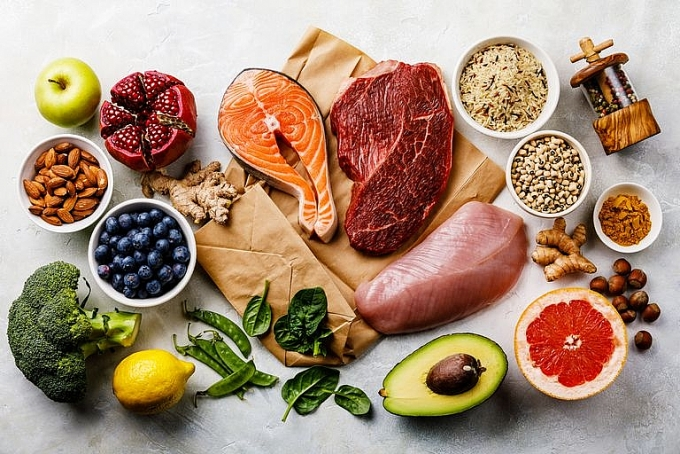
\includegraphics[width=0.7\linewidth]{images/healthy-food.jpg}
        \caption{Các chất có trong bữa ăn}
    \end{figure}
\section{Xác định ngữ cảnh của dự án UWC 2.0}
    \subsection{Các bên liên quan (Relevant Stakeholders)}
        \begin{enumerate}
            \item Công ty cung cấp dịch vụ thu dọn rác Y, ở vai trò là người quản lý.
            \item Công ty cung cấp dịch vụ thu dọn rác Y, ở vị trí là người sở hữu phần mềm UWC 2.0.
            \item Tổ chức X, phát triển phần mềm UWC 2.0.
            \item Công nhân sử dụng phần mềm UWC 2.0.
            \item Các bên liên quan khác (chính phủ, người dân).
        \end{enumerate}
    
    \subsection{Những mong muốn của các bên liên quan}
        \begin{enumerate}
            \item Công ty cung cấp dịch vụ thu dọn rác Y, ở vai trò là người quản lý, họ mong muốn phần mềm UWC 2.0 sẽ mang lại cho công ty:
            \begin{itemize}
                \item[-] Khả năng quản lý nhân lực, kiểm tra một cách hiệu quả cũng như thường xuyên cập nhật thông tin về sức chứa của các điểm tập trung rác thải (MCPs) và những thông tin nhằm phục vụ nhu cầu bảo trì các phương tiện vận chuyển, trang thiết bị của công ty.
                \item[-] Nâng cao hiệu suất thu gom rác thải của công ty.
                \item[-] Hệ thống khi được đưa vào hoạt động có độ tin cậy cao, hoạt động tốt trong mọi tình huống.
            \end{itemize}
            
            \item Công ty cung cấp dịch vụ thu dọn rác Y, ở vị trí là người sở hữu phần mềm UWC 2.0, họ sẽ có những mong muốn:
            \begin{itemize}
                \item[-] Khả năng mở rộng phạm vi hoạt động của hệ thống, không chỉ là trong một vùng, một quận cố định, mà có thể xử lý trong phạm vi toàn thành phố.
                \item[-] Chi phí và lợi nhuận luôn là một trong những vấn đề ưu tiên hàng đầu cần phải được cân nhắc. Khi được đưa vào sử dụng, UWC 2.0 phải đảm bảo tối ưu hóa về mặt nhiên liệu để từ đó giảm thiểu được chi phí phải bỏ ra. Thêm vào đó là chi phí để bảo trì hệ thống cũng phải phù hợp với công ty.
                \item[-] Trước đây công ty đã có sẵn hệ thống UWC 1.0 và công ty mong muốn có thể tận dụng lại tối đa dữ liệu có sẵn từ phiên bản trước và khả năng tương thích ngược giữa phiên bản 1.0 và 2.0.
                \item[-] Đem lại những kết quả tích cực đến công tác xử lý và tái chế rác thải trong cộng đồng, tạo ra môi trường sống xanh, sạch, đẹp cho người dân.
            \end{itemize}
      
            \item Tổ chức X, phát triển phần mềm UWC 2.0 có mong muốn:
            \begin{itemize}
                \item[-] Xây dựng được hệ thống có thể làm được và làm tốt những yêu cầu tối thiểu được yêu cầu bởi công ty chủ quản, xa hơn nữa là hoàn thiện hệ thống một cách tối ưu.
                \item[-] Hệ thống khi đến tay khách hàng phải dễ dàng bảo dưỡng, để nếu trong tương lai nếu khách hàng có thuê một công ty khác sửa chữa, bảo dưỡng hệ thống cũng thuận tiện hơn.
            \end{itemize}
        
            \item Công nhân sử dụng phần mềm UWC 2.0 mong muốn:
            \begin{itemize}
                \item[-] Vì đa phần người dùng là các cô chú trung niên, lớn tuổi, phần mềm nên có giao diện thân thiện, dễ dàng tiếp cận và làm quen.
                \item[-] Có thể sử dụng phần mềm trên nhiều thiết bị khác nhau như máy tính, điện thoại hay máy tính bảng.
                \item[-] Phần mềm phải sử dụng ổn định, ít giật lag và độ tin cậy cao.
            \end{itemize}
       
            \item Các bên liên quan khác (chính phủ, người dân): mong muốn phần mềm sẽ mang lại những ảnh hưởng tích cực đến công tác quản lý và tái sử dụng rác thải trong phạm vi khu vực và trong cả nước.
        \end{enumerate}
    
    \subsection{Vấn đề các bên liên quan đang gặp phải}
        \begin{enumerate}
            \item Công ty cung cấp dịch vụ thu dọn rác Y hiện đang gặp phải các vấn đề:
            \begin{itemize}
                \item[-] Công ty đang thiếu khả năng kiểm tra tình trạng trang thiết bị và phương tiện nên việc hoạt động chưa hiệu quả.
                \\
                \emph{\underline{Ví dụ}}: Chưa kiểm soát được tải trọng, sức chứa, tiêu thụ nhiên liệu dẫn tới sự phân bố xe chưa hợp lý khi hoạt động.
                
                \item[-] Việc quản lý nhân lực của công ty chưa hiệu quả:
                \begin{itemize}
                    \item[+] Công ty chưa theo dõi được tiến độ làm việc, hiệu suất làm việc của nhân viên.
                    \item[+] Việc phân công công việc chưa hợp lý gây mất công bằng và giảm hiệu suất công việc.
                \end{itemize}
            \end{itemize}
            
            \item Công ty cung cấp dịch vụ thu dọn rác Y, ở vị trí là người sở hữu hệ thống đang gặp phải các vấn đề:
            \begin{itemize}
                \item[-] Khả năng duy trì và nâng cấp hệ thống. Việc duy trì hệ thống đang có chi phí cao, chưa hợp lý.
                \item[-] Khi gặp các sự cố bất ngờ như  tai nạn, hư hỏng thiết bị thì việc liên lạc để điều phối nhân viên chưa kịp thời .
                \item[-] Công ty gặp bất tiện trong việc theo dõi và phân công lịch trình: lịch trình giấy, phân công thủ công. Điều này khiến công ty mất nhiều thời gian, nhân sự và việc phân công này chưa được tối ưu.
            \end{itemize}
            
            \item Các bên liên quan khác (chính phủ, người dân): Việc cải thiện môi trường chưa được tối ưu hoá, chi phí cao nhưng chưa hiệu quả dẫn đến lãng phí.
        \end{enumerate}
    
    \subsection{Lợi ích mà các bên liên quan có thể đạt được khi sử dụng hệ thống UWC 2.0}
        \begin{enumerate}
            \item Nhà cung cấp dịch vụ thu dọn rác Y ở vai trò quản lý:
            \begin{itemize}
                \item[-] Nắm bắt được cụ thể tình trạng hiện tại của các trang thiết bị và cơ sở vật chất, từ đó có thể đưa ra được những quyết định như nâng cấp, sửa chữa hay bổ sung trang thiết bị cho công nhân một cách kịp thời và hiệu quả.
                \item[-] Nhanh chóng theo dõi được tiến độ, hiệu suất làm việc của nhân viên. Đưa ra được phương án giải quyết sự cố kịp thời và công bằng.
            \end{itemize}
    
            \item Nhà cung cấp dịch vụ Y dưới góc độ chủ sở hữu hệ thống:
            \begin{itemize}
                \item[-] Tiết kiệm được chi phí duy trì và phát triển hệ thống.
                \item[-] Mang lại danh tiếng cho công ty trong mảng thu dọn rác thải.
            \end{itemize}
    
            \item Tổ chức X qua vai trò nhà phát triển phần mềm:
            \begin{itemize}
                \item[-] Tăng thu nhập cho công ty cũng như thu nhập của các cá nhân tham gia phát triển hệ thống.
                \item[-] Tăng kỹ năng của từng cá nhân.
                \item[-] Nâng cao danh tiếng, sự tin cậy cho doanh nghiệp.
            \end{itemize}
          
            \item Nhân viên  sử dụng phần mềm:
            \begin{itemize}
                \item[-] Dễ dàng sử dụng và làm quen.
                \item[-] Công sức làm việc của bản thân mỗi người được đánh giá công bằng và rõ ràng.
                \item[-] Khả năng liên lạc nhanh chóng giữa công nhân và nhân viên giám sát nhằm xử lý được những tình huống bất ngờ có thể xảy ra trong quá trình làm việc.
            \end{itemize}
            
            \item Người bị ảnh hưởng khác (chính phủ, người dân): Bảo vệ môi trường.
        \end{enumerate}
    \newpage

\section{Yêu cầu (Requirements)}
    \subsection{Yêu cầu chức năng (Functional)}
        \begin{enumerate}
            \item \textbf{Nhân viên giám sát (Back officer)}
           
            \begin{tblr}{
                width=1\linewidth,
                hlines,
                vlines,
                colspec={X[-1]X[4]X[7]},
                columns = {valign = m, },
                row{1} = {halign = c, valign = m, bg = lightgray, fg = black},
            }
                {\textbf{\#}} & \textbf{Chức năng} & {\textbf{Mô tả}} \\
                1 & Xem thông tin cá nhân & Cho phép xem chi tiết thông tin cá nhân của công nhân.\\
                2 & Xem lịch làm việc &  Xem lịch làm của từng công nhân.\\
                3 & Xem phương tiện & Xem được thông tin của từng phương tiện, các thông số kỹ thuật như trọng lượng, lượng nhiên liệu tiêu thụ, tình trạng, ...\\
                4 & Xem các điểm MCPs & Xem được thông tin các điểm MCPs, dung tích còn lại của nó.\\
                5 & Phân công công việc & Nhân viên giám sát có thể phân công công việc cho từng công nhân bao gồm việc phân phương tiện, gán các điểm MCPs và tạo tuyến đường cho công nhân lái xe rác.\\
                6 & Nhắn tin & Nhân viên giám sát có thể liên lạc với công nhân trong trường hợp bất ngờ xảy ra.\\
                7 & Thay đổi mật khẩu & Cho phép thay đổi mật khẩu trong trường hợp mong muốn hoặc thay đổi mật khẩu và có phương án xác thực dự phòng trong trường hợp quên mật khẩu.\\
                8 & Đăng nhập & Nhân viên giám sát đăng nhập vào tài khoản để sử dụng các tính năng.\\
            \end{tblr}
         
            \item \textbf{Người quản lý (Administrator)}
           
            \begin{tblr}{
                width=1\linewidth,
                hlines,
                vlines,
                colspec={X[-1]X[4]X[7]},
                columns = {valign = m, },
                row{1} = {halign = c, valign = m, bg = lightgray, fg = black},
            }
                {\textbf{\#}} & \textbf{Chức năng} & {\textbf{Mô tả}} \\
                1 & Quản lý nhân viên & Cho phép tạo, sửa, xóa một nhân viên trong hệ thống.\\
                2 & Quản lý phương tiện & Cho phép thêm, sửa, xóa một phương tiện trong hệ thống.\\
                3 & Quản lý các MCPs & Cho phép thêm, sửa, xóa các MCPs.\\
                4 & Thay đổi mật khẩu & Cho phép thay đổi mật khẩu trong trường hợp mong muốn hoặc thay đổi mật khẩu và có phương án xác thực dự phòng trong trường hợp quên mật khẩu.\\
                5 & Đăng nhập & Quản lý đăng nhập vào tài khoản để sử dụng các tính năng.\\
            \end{tblr}
           
            \newpage
            \item \textbf{Công nhân (Janitor / Collector)}
           
            \begin{tblr}{
                width=1\linewidth,
                hlines,
                vlines,
                colspec={X[-1]X[4]X[7]},
                columns = {valign = m, },
                row{1} = {halign = c, valign = m, bg = lightgray, fg = black},
            }
                {\textbf{\#}} & \textbf{Chức năng} & {\textbf{Mô tả}} \\
                1 & Xem thông tin cá nhân & Cho phép xem chi tiết thông tin cá nhân của công nhân.\\
                2 & Xem lịch làm việc & Cho phép công nhân xem lịch làm việc cụ thể trong từng ngày và tổng quát ở mỗi tuần.\\
                3 & Check in / check out & Công nhân xác nhận công việc trong ngày và đánh dấu hoàn thành công việc mỗi ngày.\\
                4 & Nhắn tin & Công nhân có thể liên lạc với văn phòng trong trường hợp bất ngờ xảy ra.\\
                5 & Nhận thông báo & Nhận thông báo mỗi khi lịch làm việc được giao cũng như tình trạng của MCPs. \\
                6 & Thay đổi mật khẩu & Cho phép thay đổi mật khẩu trong trường hợp mong muốn hoặc thay đổi mật khẩu và có phương án xác thực dự phòng trong trường hợp quên mật khẩu.\\
                7 & Đăng nhập & Công nhân đăng nhập vào tài khoản để sử dụng các tính năng.\\
            \end{tblr}
        \end{enumerate}
   
    \subsection{Yêu cầu phi chức năng (Non-functional)}
        \begin{enumerate}
            \item \textbf{Thiết kế giao diện người dùng (UI design)}
           
            \begin{tblr}{
                width=1\linewidth,
                hlines,
                vlines,
                colspec={X[-1]X[11]},
                columns = {valign = m, },
                row{1} = {halign = c, valign = m, bg = lightgray, fg = black},
            }
                {\textbf{\#}} & \textbf{Yêu cầu} \\
                1 & Thông tin quan trọng nên được hiển thị trong một lần xem (không cần kéo xuống). \\
                2 & Giao diện đơn giản. Có thể tự tìm hiểu cách sử dụng không cần hướng dẫn trong 15 phút. \\
                3 & Giao diện hệ thống: tiếng Việt và tiếng Anh cho tương lai.\\
            \end{tblr}
           
            \item \textbf{Hiệu suất (Performance)}
           
            \begin{tblr}{
                width=1\linewidth,
                hlines,
                vlines,
                colspec={X[-1]X[11]},
                columns = {valign = m, },
                row{1} = {halign = c, valign = m, bg = lightgray, fg = black},
            }
                {\textbf{\#}} & \textbf{Yêu cầu} \\
                1 & Xử lý thời gian thực với ít nhất 1000 MCPs trong thời điểm hiện tại và 10000 MCPs trong 5 năm tới.\\
                2 & Sức chứa của MCPs cần được cập nhật mỗi 15 phút. \\
                3 & Độ trễ giao tiếp thời gian thực ở dưới 1 giây. \\
                4 & Thời gian gợi ý tuyến đường tối ưu dưới 10 giây. \\
                5 & Thời gian lấy dữ liệu của công nhân dưới 5 giây. \\
            \end{tblr}
           
            \newpage
            \item \textbf{Tương thích (Compatibility)}
           
            \begin{tblr}{
                width=1\linewidth,
                hlines,
                vlines,
                colspec={X[-1]X[11]},
                columns = {valign = m, },
                row{1} = {halign = c, valign = m, bg = lightgray, fg = black},
            }
                {\textbf{\#}} & \textbf{Yêu cầu} \\
                1 & Có thể lấy và sử dụng dữ liệu cũ từ UWC 1.0.\\
                2 & Hoạt động tương thích với UWC 1.0 \\
            \end{tblr}
           
            \item \textbf{Nền tảng (Platform)}
           
            \begin{tblr}{
                width=1\linewidth,
                hlines,
                vlines,
                colspec={X[-1]X[11]},
                columns = {valign = m, },
                row{1} = {halign = c, valign = m, bg = lightgray, fg = black},
            }
                {\textbf{\#}} & \textbf{Yêu cầu} \\
                1 & Là ứng dụng web, có thể cải tiến cho ứng dụng di động trong tương lai. \\
            \end{tblr}
        \end{enumerate}
    \newpage

\section{Use-case diagram}
    

\subsection{Tổng quát của hệ thống}
    \begin{figure}[h]
        \centering
        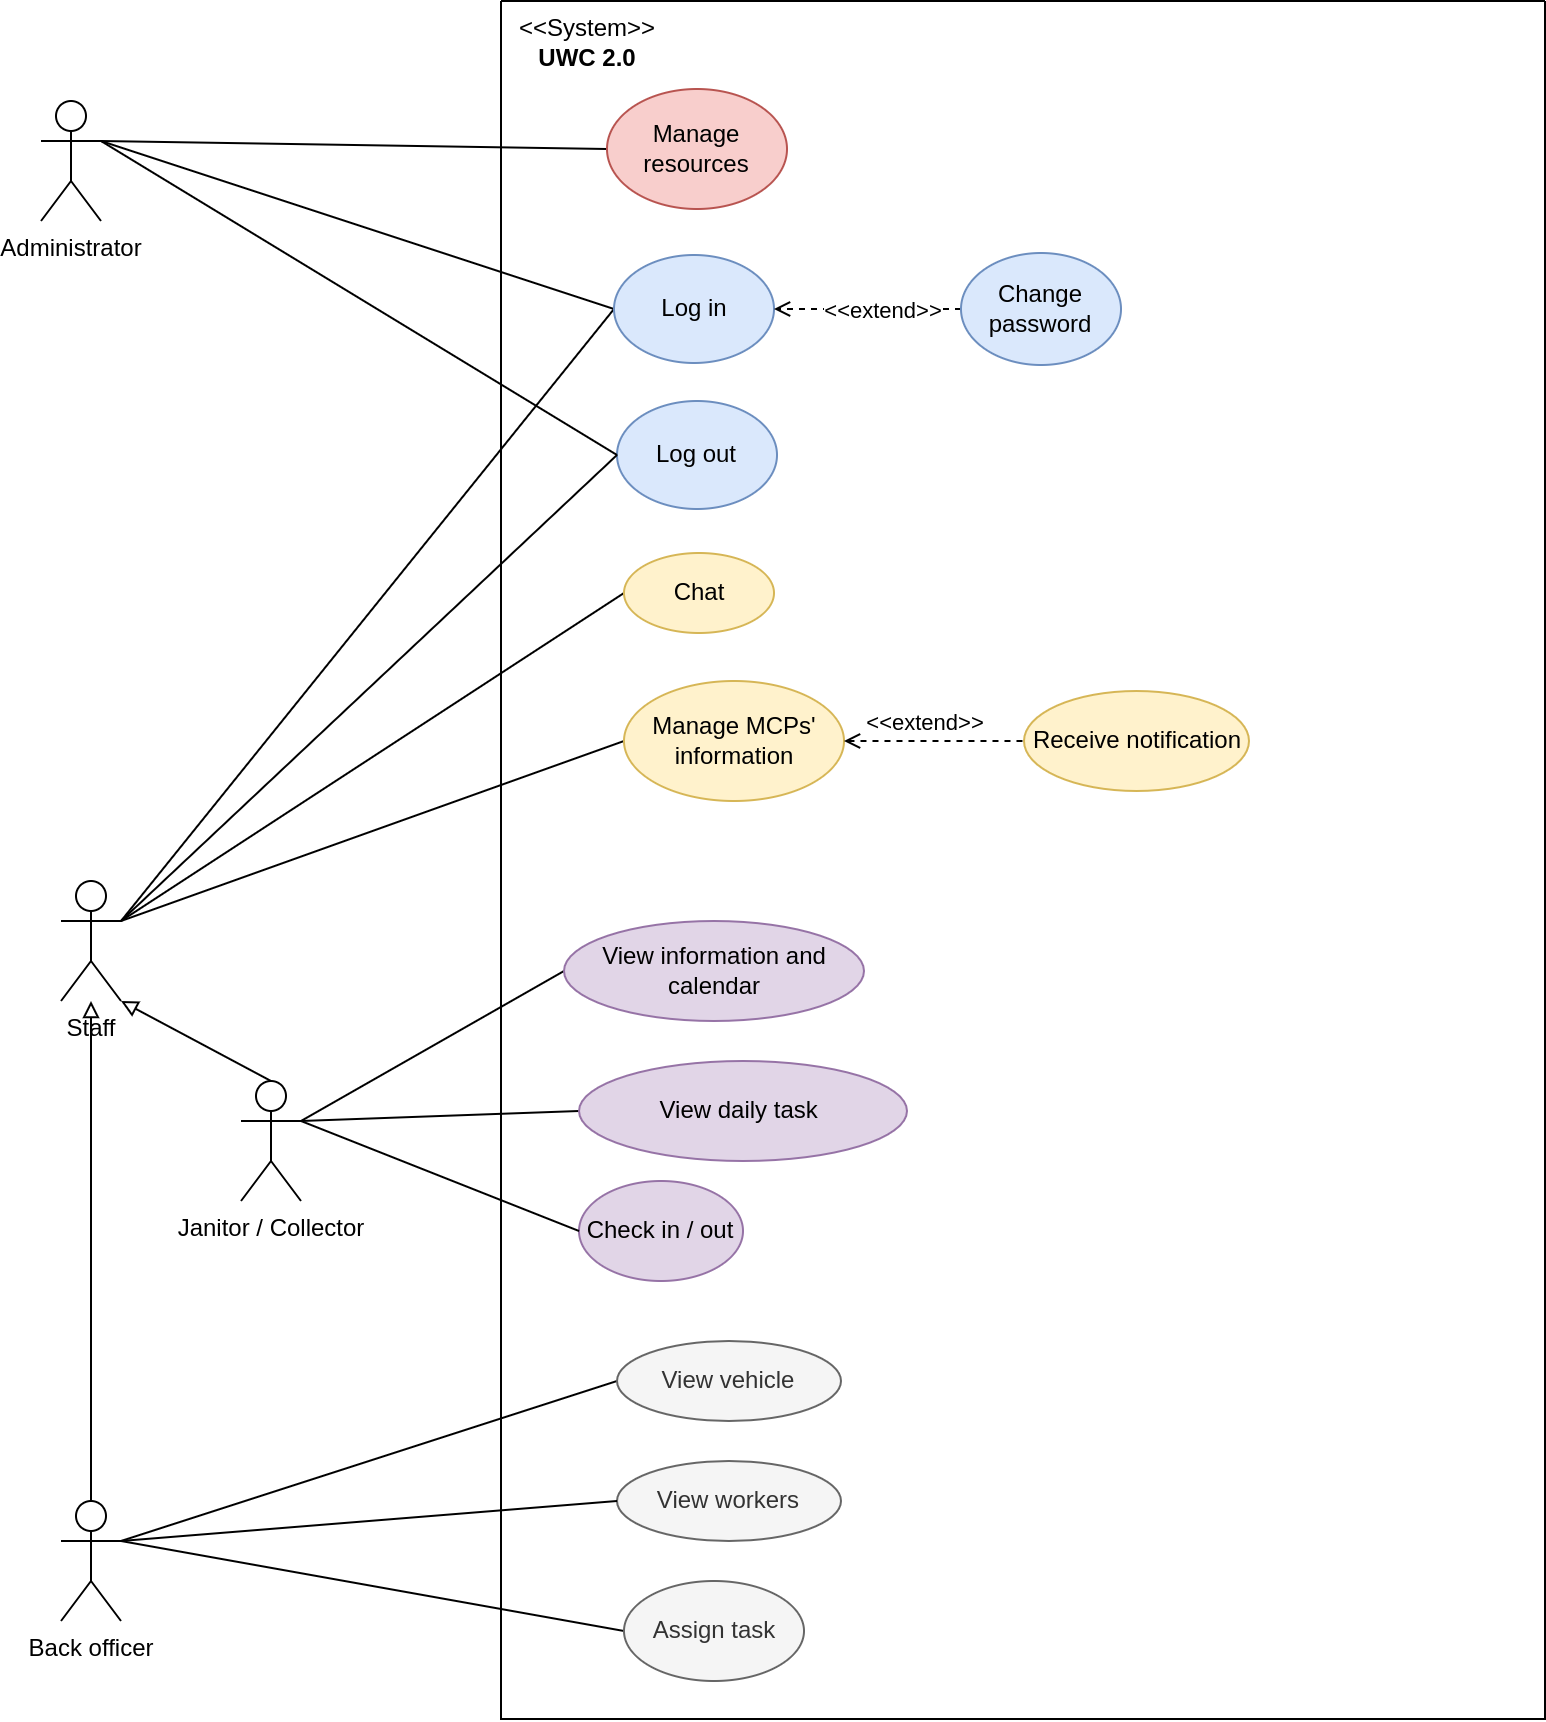
\includegraphics[width=0.93\linewidth]{imgs/use-case diagram/main_uc.png}
        \caption{Use-case diagram tổng quát của hệ thống}
    \end{figure}

    \begin{tblr}{
        width=1\linewidth,
        hlines,
        vlines,
        colspec={X[3]X[7]},
        columns = {valign = m, },
        row{1} = {halign = c, valign = m, bg = lightgray, fg = black},
    }
        {\textbf{Use case name} & \textbf{Manage resources}}  \\
        Description	& Quản lý tài nguyên của công ty \\
        Actor & Người quản lý (Administrator) \\
        Trigger & Người quản lý ấn vào phần quản lý tài nguyên  \\
        Pre-condition & Người quản lý đã đăng nhập và đang ở màn hình chính\\
        Post-condition & Người quản lý được đưa vào trang quản lý tài nguyên\\
        Normal flow &   		1. Hệ thống hiển thị giao diện quản lý tài nguyên \newline
                                2. Quản lý thực hiện việc quản lý tài nguyên \\
        Alternative flow  & 	none \\
        Exception flow & none\\
    \end{tblr}

    \vspace{1cm}

    \begin{tblr}{
        width=1\linewidth,
        hlines,
        vlines,
        colspec={X[3]X[7]},
        columns = {valign = m, },
        row{1} = {halign = c, valign = m, bg = lightgray, fg = black},
    }
        {\textbf{Use case name} & \textbf{Log in}}  \\
        Description	& Đăng nhập vào hệ thống \\
        Actor & Người quản lý (Administrator), nhân viên giám sát (Back officer), nhân viên lái xe rác (Collector), nhân viên thu gom rác (Janitor) \\
        Trigger & Người dùng mở ứng dụng  \\
        Pre-condition & Thiết bị phải có kết nối Internet\\
        Post-condition & Người dùng đăng nhập thành công\\
        Normal flow &   1. Hệ thống hiển thị giao diện đăng nhập \newline
                    	2. Người dùng ghi thông tin về tên tài khoản và mật khẩu \newline
                    	3. Hệ thống kiểm tra thông tin được ghi \newline
                    	4. Hệ thống thông báo đăng nhập thành công \newline
                    	5. Hệ thống hiển thị giao diện màn hình chính \\
        Alternative flow  & Alternative flow thứ 1: tại bước 2 \newline
                        	1a. Người dùng chọn lưu tài khoản \newline
                        	Tiếp tục bước 3 \newline
                        	1b. Hệ thống lưu lại tài khoản \newline
                        	Tiếp tục bước 4 \\
        Exception flow & 	Exception flow thứ 1: tại bước 3 \newline
                        	1a. Nếu không tìm thấy tài khoản, sai mật khẩu, thông báo cho người dùng \newline
                        	Quay lại bước 2 \\
        Extended points & Change password \\
    \end{tblr}

    \vspace{1cm}
    \begin{tblr}{
        width=1\linewidth,
        hlines,
        vlines,
        colspec={X[3]X[7]},
        columns = {valign = m, },
        row{1} = {halign = c, valign = m, bg = lightgray, fg = black},
    }
        {\textbf{Use case name} & \textbf{Change password}}  \\
        Description	& Thay đổi mật khẩu của tài khoản \\
        Actor & Người quản lý (Administrator), nhân viên giám sát (Back officer), nhân viên lái xe rác (Collector), nhân viên thu gom rác (Janitor) \\
        Trigger & Người dùng ấn vào nút quên mật khẩu  \\
        Pre-condition & Người dùng đang ở phần đăng nhập \\
        Post-condition & Mật khẩu được thay đổi thành công \\
        Normal flow &   1. Hệ thống hiển thị thay giao diện thay đổi mật khẩu \newline
                    	2. Người dùng nhập tên tài khoản \newline
                    	3. Hệ thống kiểm tra tài khoản \newline
                    	4. Người dùng nhập mã mật khẩu mới \newline
                    	5. Hệ thống kiểm tra mật khẩu mới \newline
                    	6. Hệ thống thông báo đổi mật khẩu thành công \newline
                    	7. Hệ thống quay lại trang đăng nhập \\
        Alternative flow  & none \\
        Exception flow & 	Exception flow thứ 1: tại bước 3 \newline
                            1a. Nếu tài khoản không tồn tại, thông báo cho người dùng \newline
                            Quay lại bước 2 \newline

                            Exception flow thứ 2: tại bước 5 \newline
                            2a. Nếu mật khẩu không đúng quy đinh, thông báo cho người dùng \newline
                            Quay lại bước 4 \\
    \end{tblr}

    \vspace{1cm}
    \begin{tblr}{
        width=1\linewidth,
        hlines,
        vlines,
        colspec={X[3]X[7]},
        columns = {valign = m, },
        row{1} = {halign = c, valign = m, bg = lightgray, fg = black},
    }
        {\textbf{Use case name} & \textbf{Log out}}  \\
        Description	& Đăng xuất khỏi phiên làm việc \\
        Actor & Người quản lý (Administrator), nhân viên giám sát (Back officer), nhân viên lái xe rác (Collector), nhân viên thu gom rác (Janitor) \\
        Trigger & Người dùng ấn vào nút đăng xuất  \\
        Pre-condition & Người dùng đã đăng nhập, và đang ở màn hình chính \\
        Post-condition & Tài khoản được đăng xuất khỏi hệ thống \\
        Normal flow &   1. Người dùng ấn vào menu \newline
                    	2. Người dùng chọn đăng xuất \newline
                    	3. Hệ thống hiện thị form xác nhận đăng xuất \newline
                    	4. Hệ thống xóa phiên làm việc  \newline
                    	5. Hệ thống quay trở lại trang đăng nhập \\
        Alternative flow  & Alternative flow thứ 1: tại bước 3 \newline
                            1a. Nếu người dùng chọn hủy, quay lại màn hình chính \\
        Exception flow & none\\
    \end{tblr}

    \begin{tblr}{
        width=1\linewidth,
        hlines,
        vlines,
        colspec={X[3]X[7]},
        columns = {valign = m, },
        row{1} = {halign = c, valign = m, bg = lightgray, fg = black},
    }
        {\textbf{Use case name} & \textbf{Chat}}  \\
        Description	& Nhân viên liên lạc với nhau \\
        Actor & Nhân viên (Staff) \\
        Trigger & 	Nhân viên ấn vào phần liên hệ \\
        Pre-condition & Người dùng đã đăng nhập\\
        Post-condition & Tin nhắn được gửi thành công \newline
                         Nhân viên nhận và đọc được tin nhắn \\
        Normal flow &   1. Hệ thống lấy thông tin về các nhân viên \newline
                    	2. Hệ thống hiển thị danh sách các nhân viên \newline
                    	3. Người dùng chọn nhân viên muốn liên hệ \newline
                    	4. Hệ thống hiển thị giao diện nhắn tin \newline
                    	5. Người dùng nhập tin nhắn \newline
                    	6. Người dùng nhấn gửi \newline
                    	7. Hệ thống ghi nhận tin nhắn và gửi cho người được nhắn \\
        Alternative flow  & none \\
        Exception flow & none \\
    \end{tblr}

    \vspace{1cm}
    \begin{tblr}{
        width=1\linewidth,
        hlines,
        vlines,
        colspec={X[3]X[7]},
        columns = {valign = m, },
        row{1} = {halign = c, valign = m, bg = lightgray, fg = black},
    }
        {\textbf{Use case name} & \textbf{Manage MCP's information}}  \\
        Description	& Xem thông tin về các MCPs \\
        Actor & Nhân viên (Staff) \\
        Trigger & 	Nhân viên ấn vào mục tổng quan MCPs \\
        Pre-condition & Nhân viên đã đăng nhập và đang ở màn hình chính \\
        Post-condition & Thông tin về MCP được hiển thị thành công \\
        Normal flow &   1. Hệ thống lấy thông tin các MCPs \newline
                    	2. Hệ thống hiện thị danh sách các MCPs \newline
                    	3. Nhân viên chọn 1 MCP bất kì \newline
                    	4. Hệ thống hiển thị thông tin chi tiết của MCPs vừa được chọn \\
        Alternative flow  & none \\
        Exception flow & none \\
        Extended points & Receive notification \\
    \end{tblr}

    \begin{tblr}{
        width=1\linewidth,
        hlines,
        vlines,
        colspec={X[3]X[7]},
        columns = {valign = m, },
        row{1} = {halign = c, valign = m, bg = lightgray, fg = black},
    }
        {\textbf{Use case name} & \textbf{Receive notification}}  \\
        Description	& Cập nhật tình trạng của MCP \\
        Actor & Nhân viên (Staff) \\
        Trigger & none \\
        Pre-condition & Nhân viên đã đăng nhập \\
        Post-condition & Thông báo được nhận bởi nhân viên \\
        Normal flow &   1. Hệ thống truy cập vào dữ liệu về MCPs \newline
                    	2. Hệ thống lấy thông tin về dung tích của MCPs \newline
                    	3. Hệ thống gửi thông báo về cho người dùng \newline
                    	4. Người dùng nhận được thông báo \\
        Alternative flow  & none \\
        Exception flow & none \\
    \end{tblr}

    \vspace{1cm}
    \begin{tblr}{
        width=1\linewidth,
        hlines,
        vlines,
        colspec={X[3]X[7]},
        columns = {valign = m, },
        row{1} = {halign = c, valign = m, bg = lightgray, fg = black},
    }
        {\textbf{Use case name} & \textbf{View information and calendar}}  \\
        Description	& Công nhân xem thông tin và lịch làm trong tuần \\
        Actor & 	Nhân viên lái xe rác (Collector), Nhân viên thu gom rác (Janitor) \\
        Trigger & 	Công nhân ấn vào phần thông tin và lịch làm \\
        Pre-condition & Công nhân đã đăng nhập và đang ở màn hình chính \\
        Post-condition & Công nhân xem được thông tin và lịch làm của mình \\
        Normal flow &   1. Hệ thống lấy thông tin và lịch làm \newline
                    	2. Hệ thống hiển thị giao diện bao gồm 2 tab (thông tin chung, lịch làm) 	mặc định ở thông tin chung \newline
                    	3. Công nhân xem thông tin của bản thân\\
        Alternative flow  & Alternative flow thứ 1: Tại bước 2 \newline
                    	    1a. Người dùng chọn tab lịch làm \newline
                    	    1b. Hệ thống hiển thị giao diện về lịch làm việc trong tuần \\
        Exception flow & none \\
    \end{tblr}

    \begin{tblr}{
        width=1\linewidth,
        hlines,
        vlines,
        colspec={X[3]X[7]},
        columns = {valign = m, },
        row{1} = {halign = c, valign = m, bg = lightgray, fg = black},
    }
        {\textbf{Use case name} & \textbf{View daily task}}  \\
        Description	& Công nhân xem chi tiết công việc trong ngày \\
        Actor & 	Nhân viên lái xe rác (Collector), Nhân viên thu gom rác (Janitor) \\
        Trigger & 	Công nhân ấn vào phần nhiệm vụ hôm nay\\
        Pre-condition & Công nhân đã đăng nhập và đang ở màn hình chính \\
        Post-condition & Nhiệm vụ cụ thể trong ngày được hiện lên màn hình \\
        Normal flow &   1. Hệ thống lấy thông tin làm việc trong ngày \newline
                    	2. Hệ thống hiển thị thông tin làm việc \newline
                    	3. Người dùng đọc được thông tin làm việc\\
        Alternative flow  & none \\
        Exception flow & none \\
    \end{tblr}

    \vspace{1cm}
    \begin{tblr}{
        width=1\linewidth,
        hlines,
        vlines,
        colspec={X[3]X[7]},
        columns = {valign = m, },
        row{1} = {halign = c, valign = m, bg = lightgray, fg = black},
    }
        {\textbf{Use case name} & \textbf{Check in/out}}  \\
        Description	& Nhận và đánh dấu hoàn thành công việc \\
        Actor & 	Nhân viên lái xe rác (Collector), Nhân viên thu gom rác (Janitor) \\
        Trigger & 		Công nhân chọn nhận công việc \\
        Pre-condition & Công nhân đang ở phần thông tin nhiệm vụ chi tiết \\
        Post-condition & Nhiệm vụ được nhận / được hoàn thành \\
        Normal flow &   1. Công nhân xác nhận nhiệm vụ \newline
                        2. Hệ thống ghi nhận công nhân đã xác nhận \\
        Alternative flow  & Alternative flow thứ 1: tại bước 1 \newline
                        	1a. Công nhân ấn hoàn thành nhiệm vụ \newline
                        	1b. Hệ thống ghi nhận \\
        Exception flow & none \\
    \end{tblr}

    \begin{tblr}{
        width=1\linewidth,
        hlines,
        vlines,
        colspec={X[3]X[7]},
        columns = {valign = m, },
        row{1} = {halign = c, valign = m, bg = lightgray, fg = black},
    }
        {\textbf{Use case name} & \textbf{View workers}}  \\
        Description	& Xem thông tin công nhân và lịch làm của họ \\
        Actor & 	Nhân viên giám sát (Back officer) \\
        Trigger & 	Nhân viên giám sát ấn vào mục quản lý nhân viên \\
        Pre-condition & Nhân viên giám sát đã đăng nhập và đang ở màn hình chính \\
        Post-condition & Thông tin chi tiết và lịch làm việc trong tuần của công nhân được hiển thị \\
        Normal flow &   1. Hệ thống lấy dữ liệu của nhân viên \newline
                    	2. Hệ thống hiển thị danh sách tên các nhân viên \newline
                    	3. Nhân viên giám sát chọn một nhân viên \newline
                    	4. Hệ thống hiển thị thông tin chi tiết của nhân viên \\
        Alternative flow  & Alternative flow thứ 1: tại bước 4 \newline
                        	1a. Người dùng chọn qua mục lịch làm việc \newline
                        	1b. Hệ thống lấy thông tin về lịch làm việc của nhân viên \newline
                        	1c. Hệ thống hiển thị lên màn hình \\
        Exception flow & none \\
    \end{tblr}

    \vspace{1cm}
    \begin{tblr}{
        width=1\linewidth,
        hlines,
        vlines,
        colspec={X[3]X[7]},
        columns = {valign = m, },
        row{1} = {halign = c, valign = m, bg = lightgray, fg = black},
    }
        {\textbf{Use case name} & \textbf{View vehicle}}  \\
        Description	& Xem thông tin của các phương tiện \\
        Actor & 	Nhân viên giám sát (Back officer) \\
        Trigger & 	Nhân viên giám sát ấn vào mục theo dõi phương tiện\\
        Pre-condition & Nhân viên giám sát đã đăng nhập và đang ở màn hình chính \\
        Post-condition & Thông tin phương tiện được hiển thị trên màn hình \\
        Normal flow &   1. Hệ thống truy cập vào dữ liệu về phương tiện \newline
                    	2. Hệ thống hiển thị các phương tiện \newline
                    	3. Người dùng chọn một phương tiện bất kì \newline
                    	4. Hệ thống hiện thị thông tin chi tiết của phương tiện \\
        Alternative flow  & none \\
        Exception flow & none \\
    \end{tblr}
    \newpage

    
\subsection{Chức năng phân chia công việc (Task assignment)}
    \begin{figure}[h]
        \centering
        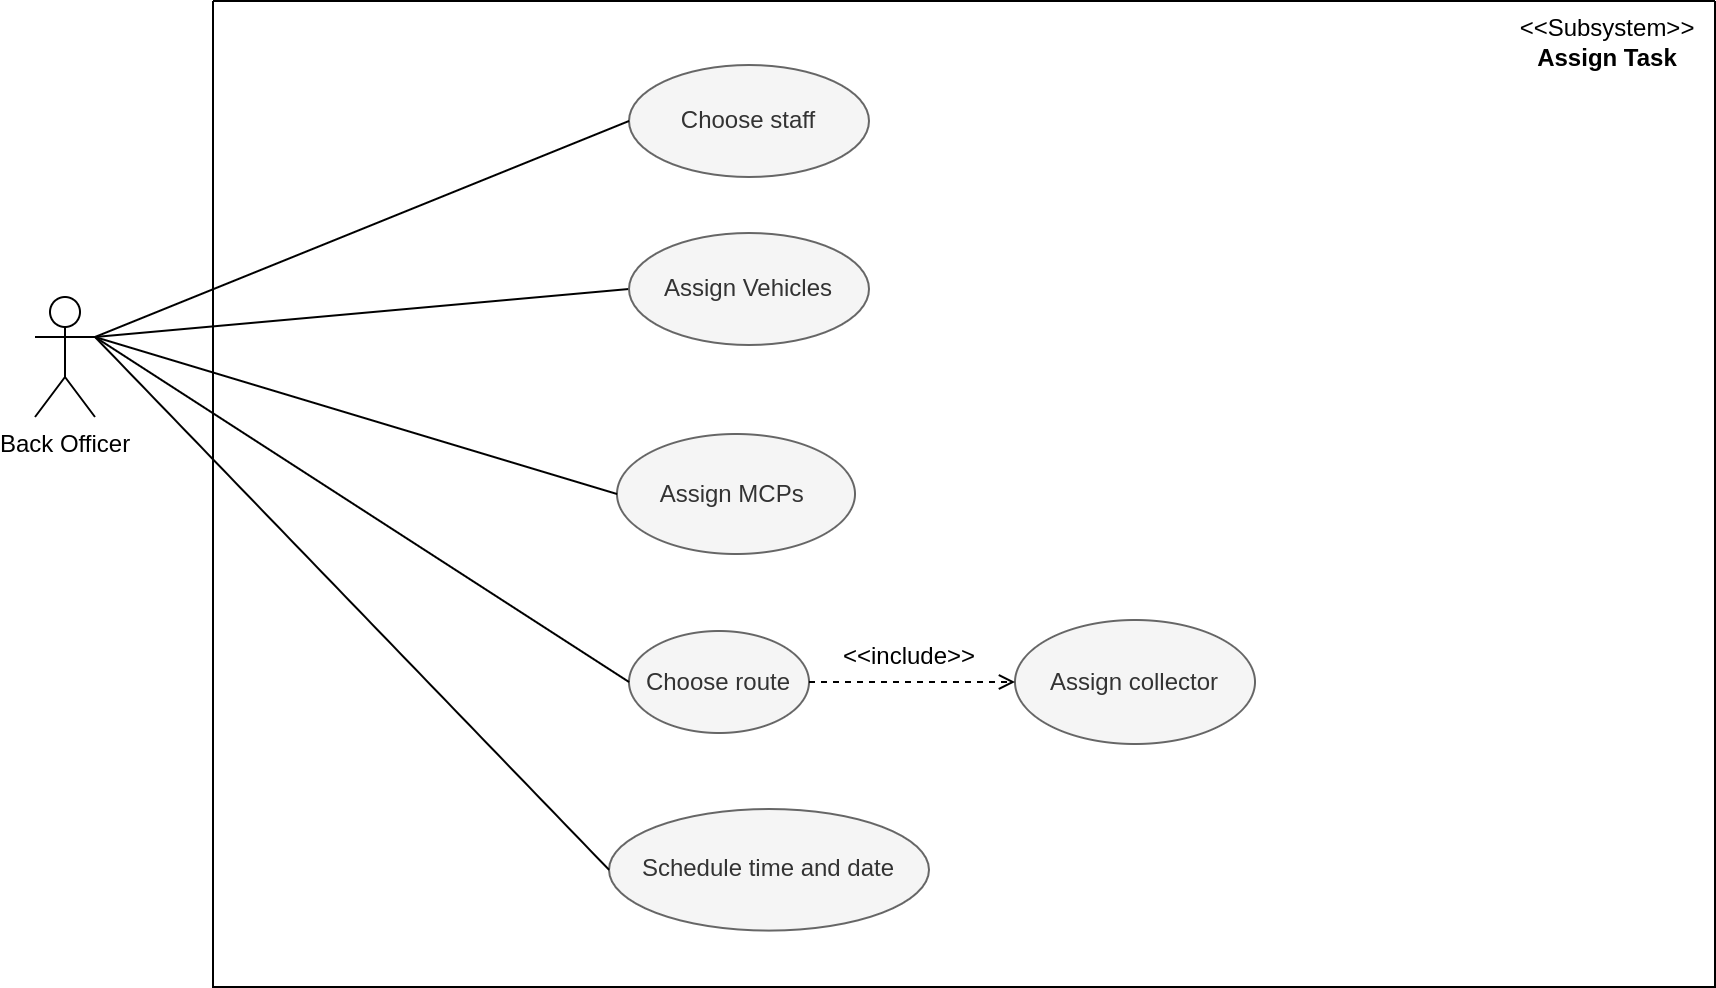
\includegraphics[width=1\linewidth]{imgs/use-case diagram/assignTask_uc.png}
        \caption{Use-case diagram chức năng phân chia công việc}
    \end{figure}

    \vspace{1cm}
    \begin{tblr}{
        width=1\linewidth,
        hlines,
        vlines,
        colspec={X[3]X[7]},
        columns = {valign = m, },
        row{1} = {halign = c, valign = m, bg = lightgray, fg = black},
    }
        {\textbf{Use case name} & \textbf{Choose staff}}  \\
        Description	& Chọn một nhân viên trong hệ thống \\
        Actor & 	Nhân viên giám sát (Back officer) \\
        Trigger & 		Nhân viên giám sát ấn nút chọn công nhân\\
        Pre-condition & Nhân viên giám sát đang ở phần phân công công việc \\
        Post-condition & Công nhân được chọn \\
        Normal flow &   1. Hệ thống lấy dữ liệu về công nhân \newline
                    	2. Hệ thống hiển thị các công nhân \newline
                    	3. Nhân viên giám sát chọn công nhân \newline
                    	4. Hệ thống ghi nhận công nhân được chọn \\
        Alternative flow  & none \\
        Exception flow & none \\
    \end{tblr}

    \begin{tblr}{
        width=1\linewidth,
        hlines,
        vlines,
        colspec={X[3]X[7]},
        columns = {valign = m, },
        row{1} = {halign = c, valign = m, bg = lightgray, fg = black},
    }
        {\textbf{Use case name} & \textbf{Choose vehicle}}  \\
        Description	& Chọn một phương tiện có trong công ty \\
        Actor & 	Nhân viên giám sát (Back officer) \\
        Trigger & 		Nhân viên giám sát ấn nút chọn công nhân\\
        Pre-condition & Nhân viên giám sát đang ở phần phân công công việc \\
        Post-condition & Phương tiện được chọn thành công \\
        Normal flow &   1. Hệ thống lấy dữ liệu về phương tiện \newline
                    	2. Hệ thống hiển thị các phương tiện \newline
                    	3. Nhân viên giám sát chọn phương tiện \newline
                    	4. Hệ thống kiểm tra phương tiện đã được lái hay chưa \newline
                    	5. Hệ thống ghi nhận phương tiện được chọn \\
        Alternative flow  & none \\
        Exception flow & Exception flow thứ 1: tại bước 4 \newline
                    	 1a. Nếu phương tiện đã được gán, thông báo cho người dùng \newline
                    	 Quay lại bước 2 \\
    \end{tblr}

    \vspace{1cm}
    \begin{tblr}{
        width=1\linewidth,
        hlines,
        vlines,
        colspec={X[3]X[7]},
        columns = {valign = m, },
        row{1} = {halign = c, valign = m, bg = lightgray, fg = black},
    }
        {\textbf{Use case name} & \textbf{Assign MCPs}}  \\
        Description	& Gán các điểm MCP cho công nhân \\
        Actor & 	Nhân viên giám sát (Back officer) \\
        Trigger & 	Nhân viên giám sát ấn nút chọn MCPs\\
        Pre-condition & Người quản lý đang ở phần phân công công việc \\
        Post-condition & Các điểm MCP được phân công thành công\\
        Normal flow &   1. Hệ thống lấy dữ liệu về các MCP \newline
                    	2. Hệ thống hiển thị các MCP \newline
                    	3. Nhân viên giám sát chọn MCP \newline
                    	4. Hệ thống ghi nhận các MCP được chọn \\
        Alternative flow  & Alternative flow thứ 1: tại bước 3 \newline
                        	1a. Nếu công nhân được chọn là collector, cho phép gán nhiều MCP \newline
                            \newline
                        	Alternative flow thứ 2: tại bước 3 \newline
                        	2a. Nếu công nhân được chọn là janitor, cho phép gán chỉ 1 MCP \\
        Exception flow & none \\
    \end{tblr}

    \begin{tblr}{
        width=1\linewidth,
        hlines,
        vlines,
        colspec={X[3]X[7]},
        columns = {valign = m, },
        row{1} = {halign = c, valign = m, bg = lightgray, fg = black},
    }
        {\textbf{Use case name} & \textbf{Choose route}}  \\
        Description	& Chọn tuyến đường cho collector \\
        Actor & 	Nhân viên giám sát (Back officer) \\
        Trigger & 	Nhân viên giám sát ấn nút chọn tuyến đường \\
        Pre-condition & Người quản lý đang ở phần phân công công việc \\
        Post-condition & Tuyến đường được chọn\\
        Normal flow &   1. Hệ thống kiểm tra công nhân được chọn là ai \newline
                    	2. Hệ thống hiển thị map trong thành phố \newline
                    	3. Hệ thống hiển thị các tuyến đường được xem là tối ưu \newline
                    	4. Nhân viên giám sát chọn tuyến đường \newline
                    	5. Hệ thống ghi nhận tuyến đường được chọn \\
        Alternative flow  & Alternative flow thứ 1: tại bước 1 \newline
                            1a. Nếu công nhân được chọn là Janitor, hệ thống thông báo và quay 	trở lại màn hình phân công công việc \\
        Exception flow & none \\
    \end{tblr}

    \vspace{1cm}
    \begin{tblr}{
        width=1\linewidth,
        hlines,
        vlines,
        colspec={X[3]X[7]},
        columns = {valign = m, },
        row{1} = {halign = c, valign = m, bg = lightgray, fg = black},
    }
        {\textbf{Use case name} & \textbf{Schedule time and date}}  \\
        Description	& Xếp lịch cho nhân viên \\
        Actor & 	Nhân viên giám sát (Back officer) \\
        Trigger & 	Nhân viên giám sát ấn nút set lịch làm\\
        Pre-condition & Người quản lý đang ở phần phân công công việc \\
        Post-condition & Lịch làm được phân thành công\\
        Normal flow &   1. Hệ thống lấy dữ liệu về lịch làm \newline
                    	2. Hệ thống hiển thị các ngày trong tuần \newline
                    	3. Nhân viên giám sát chọn các ca còn trống \newline
                    	4. Nhân viên xác nhận lịch đã chọn \newline
                    	5. Hệ thống ghi nhận lịch làm \\
        Alternative flow  & none \\
        Exception flow & none \\
    \end{tblr}

\newpage

    

\subsection{Chức năng quản lý tài nguyên (Manage Resources)}
    \begin{figure}[h]
        \centering
        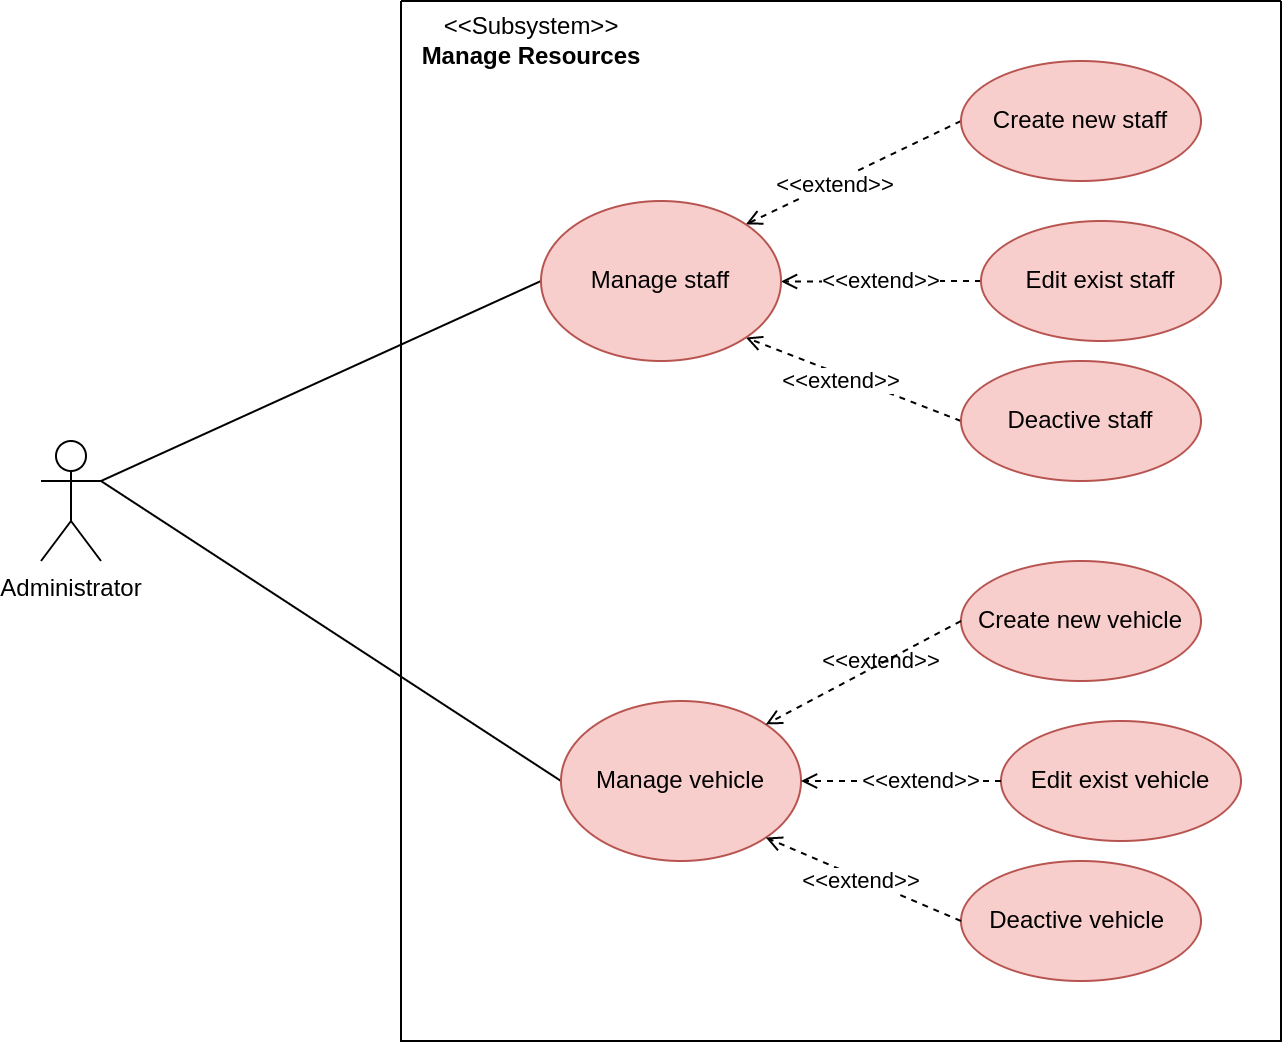
\includegraphics[width=0.70\linewidth]{imgs/use-case diagram/manageResources_uc.png}
        \caption{Use-case diagram chức năng kiểm soát tài nguyên}
    \end{figure}

    \vspace{1cm}
    \begin{tblr}{
        width=1\linewidth,
        hlines,
        vlines,
        colspec={X[3]X[7]},
        columns = {valign = m, },
        row{1} = {halign = c, valign = m, bg = lightgray, fg = black},
    }
        {\textbf{Use case name} & \textbf{Manage staff}}  \\
        Description	& Xếp lịch cho nhân viên \\
        Actor & 	Người quản lý (Administrator) \\
        Trigger & 	Người quản lý ấn vào phần quản lý nhân viên ở menu chính \\
        Pre-condition & Người quản lý đang ở quản lý tài nguyên \\
        Post-condition & Trang quản lý nhân viên được hiển thị \\
        Normal flow &   1. Hệ thống lấy dữ liệu về các nhân viên\newline
                    	2. Hệ thống hiện thị danh sách nhân viên lên màn hình \newline
                    	3. Người dùng chọn một nhân viên để thực hiện hành động \newline
                     	4. Hệ thống hiện thị thông tin chi tiết của nhân viên \\
        Extended points & 	Create new staff \newline
                        	Edit exist staff \newline
                        	Deactive staff \\
    \end{tblr}

    \begin{tblr}{
        width=1\linewidth,
        hlines,
        vlines,
        colspec={X[3]X[7]},
        columns = {valign = m, },
        row{1} = {halign = c, valign = m, bg = lightgray, fg = black},
    }
        {\textbf{Use case name} & \textbf{Create new staff}}  \\
        Description	& Tạo ra một nhân viên mới \\
        Actor & 	Người quản lý (Administrator) \\
        Trigger & 	Người quản lý ấn vào nút tạo người dùng mới \\
        Pre-condition & Người quản lý đang ở trong phần quản lý nhân viên \\
        Post-condition & Nhân viên mới được tạo ra \\
        Normal flow &   1. Hệ thống hiển thị các thông tin cần điền \newline
                    	2. Người dùng điền các thông tin \newline
                    	3. Hệ thống kiểm tra thông tin được điền \newline
                    	4. Người dùng ấn tạo nhân viên mới \newline
                    	5. Hệ thống ghi nhận nhân viên mới \newline
                    	6. Hệ thống thông báo tạo nhân viên thành công \\
        Alternative flow  & Alternative flow thứ 1: tại bước 1 \newline
                        	1a. Người dùng ấn nút hủy \newline
                        	1b. Quay lại màn hình thông tin chi tiết của nhân viên \\
        Exception flow & Exception flow thứ 1: tại bước 3 \newline
                    	 1a. Nếu thông tin sai, thông báo cho người dùng \newline
                    	 Quay lại bước 2  \\
    \end{tblr}

    \vspace{1cm}
    \begin{tblr}{
        width=1\linewidth,
        hlines,
        vlines,
        colspec={X[3]X[7]},
        columns = {valign = m, },
        row{1} = {halign = c, valign = m, bg = lightgray, fg = black},
    }
        {\textbf{Use case name} & \textbf{Edit exist staff}}  \\
        Description	& Chỉnh sửa một nhân viên  \\
        Actor & 	Người quản lý (Administrator) \\
        Trigger & 	Người quản lý ấn vào nút chỉnh sửa nhân viên \\
        Pre-condition & Người quản lý đang ở trong phần quản lý nhân viên \\
        Post-condition & Thông tin nhân viên được chỉnh sửa thành công\\
        Normal flow &   1. Hệ thống hiển thị các thông tin cần điền \newline
                    	2. Người dùng điền các thông tin \newline
                    	3. Hệ thống kiểm tra thông tin được điền \newline
                    	4. Người dùng ấn cập nhật nhân viên \newline
                    	5. Hệ thống ghi nhận thông tin được cập nhật \newline
                    	6. Hệ thống thông báo cập nhật nhân viên thành công \\
        Alternative flow  & Alternative flow thứ 1: tại bước 1 \newline
                        	1a. Người dùng ấn nút hủy \newline
                        	1b. Quay lại màn hình thông tin chi tiết của nhân viên \\
        Exception flow & Exception flow thứ 1: tại bước 3 \newline
                    	 1a. Nếu thông tin sai, thông báo cho người dùng \newline
                    	 Quay lại bước 2 \\
    \end{tblr}

    \begin{tblr}{
        width=1\linewidth,
        hlines,
        vlines,
        colspec={X[3]X[7]},
        columns = {valign = m, },
        row{1} = {halign = c, valign = m, bg = lightgray, fg = black},
    }
        {\textbf{Use case name} & \textbf{Deactive staff}}  \\
        Description	& Hủy kích hoạt một nhân viên \\
        Actor & 	Người quản lý (Administrator) \\
        Trigger & 	Người quản lý ấn vào nút hủy kích hoạt nhân viên \\
        Pre-condition & Người quản lý đang ở trong phần quản lý nhân viên \\
        Post-condition & Nhân viên bị hủy kích hoạt\\
        Normal flow &   1. Hệ thống hiểu thị xác nhận hủy kích hoạt nhân viên \newline
                    	2. Người dùng nhấn đồng ý \newline
                    	3. Hệ thống hủy kích hoạt nhân viên \newline
                    	4. Hệ thống thông báo hủy kích hoạt thành công \\
        Alternative flow  & Alternative flow thứ 1: tại bước 1 \newline
                        	1a. Người dùng ấn nút hủy \newline
                        	1b. Quay lại màn hình thông tin chi tiết của nhân viên \\
        Exception flow & none \\
    \end{tblr}

    \vspace{1cm}
    \quad Phần use-case senario của  Manage vehicle tương tự như trên.


	
\section{Activity diagram giữa hệ thống và các bên liên quan trong Task Assignment Module}
    \begin{figure}[h]
        \centering
        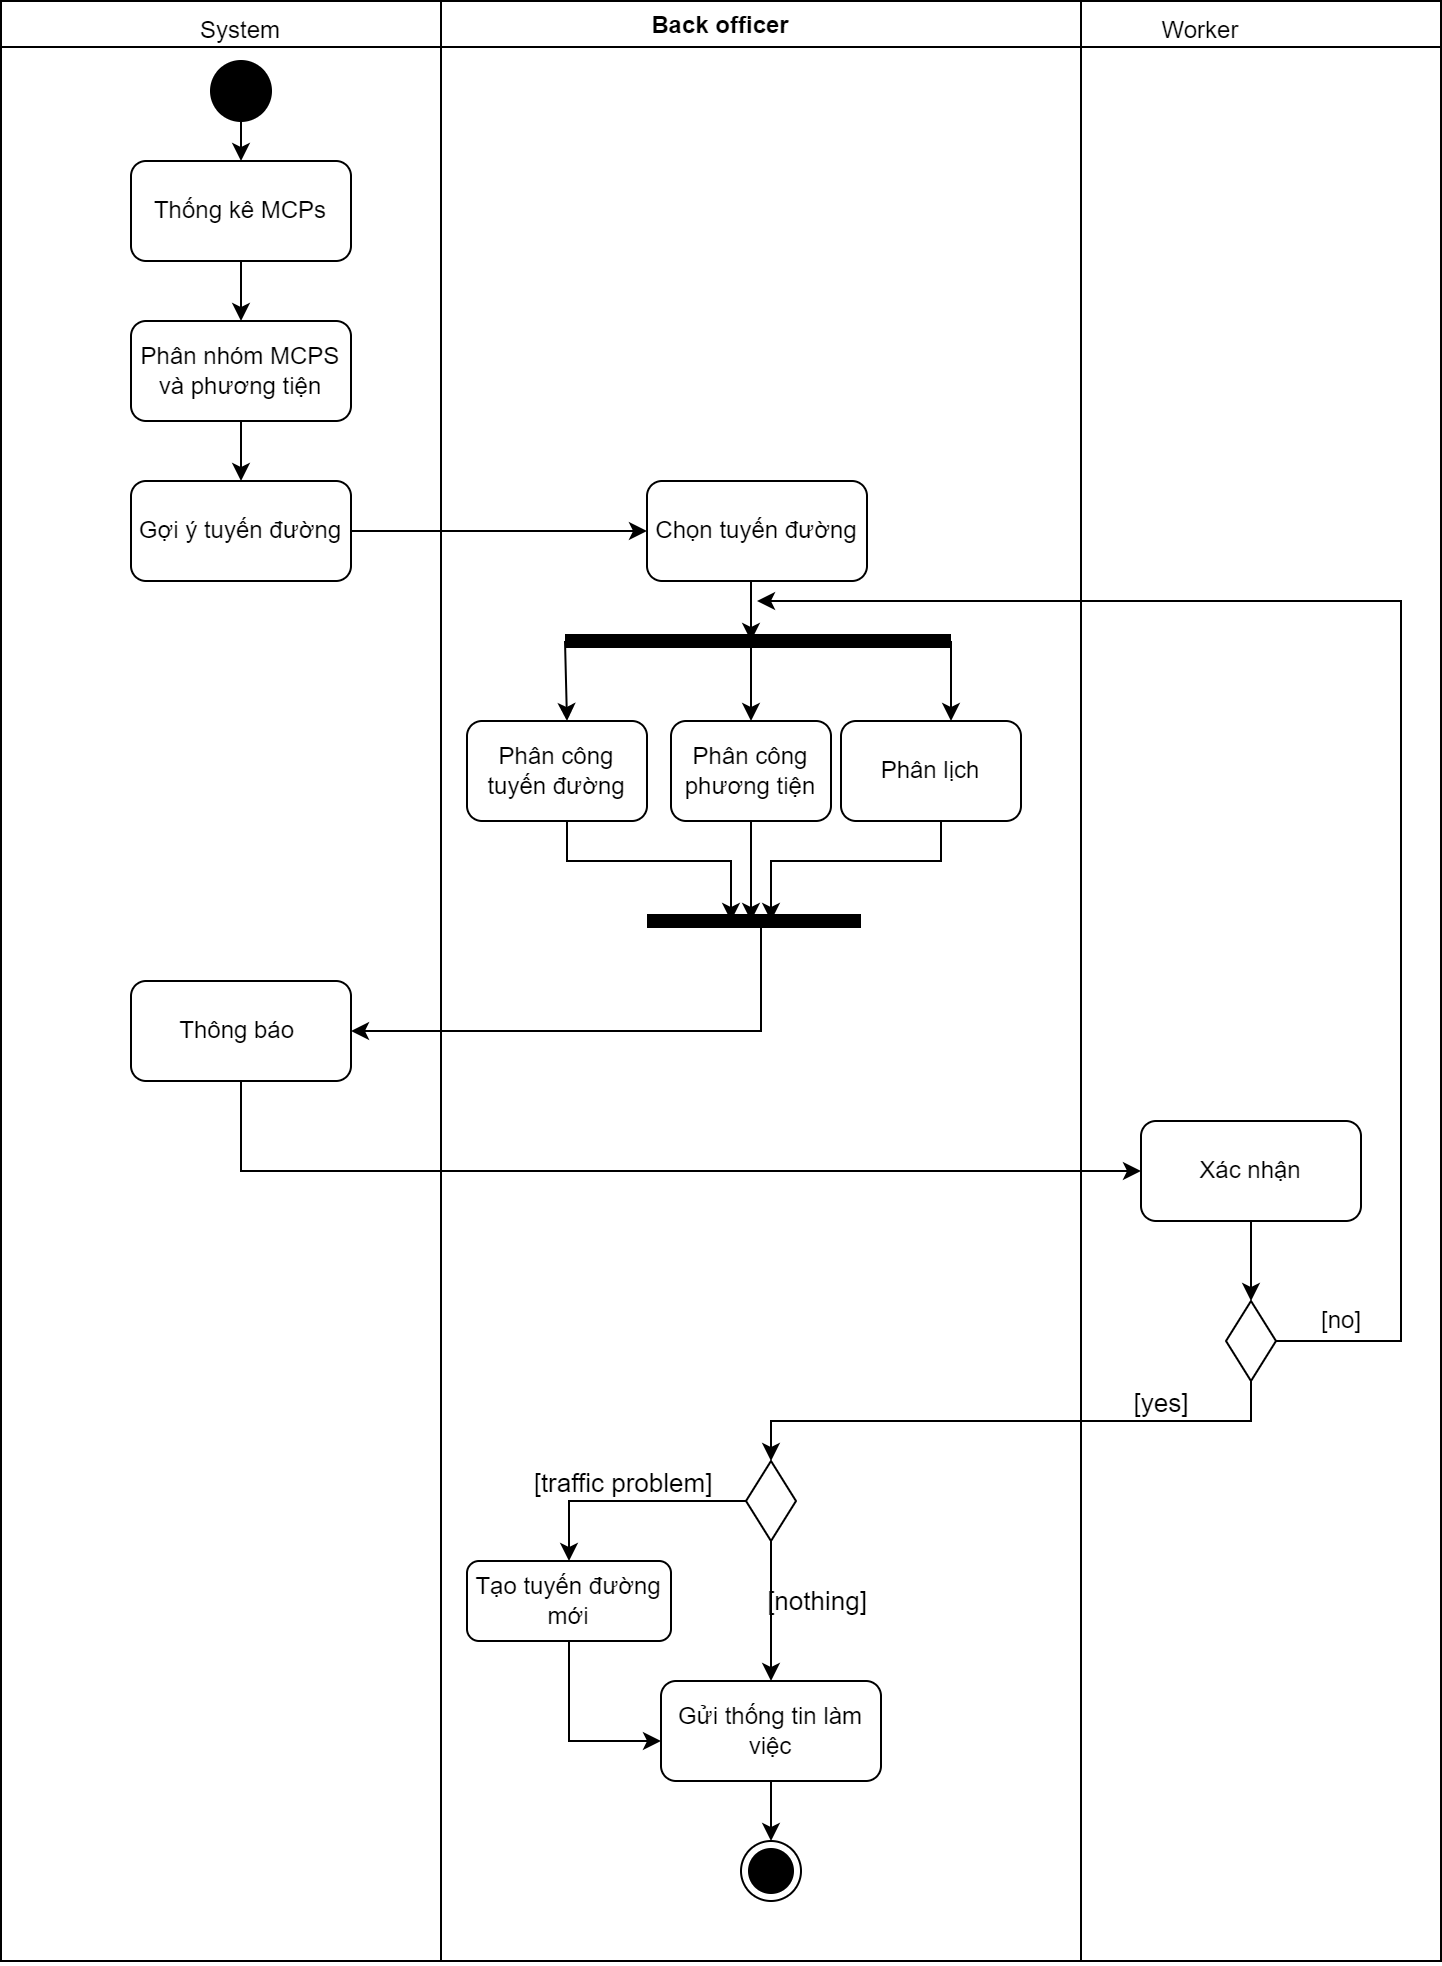
\includegraphics[width=15.0cm,height=15cm]{imgs/activity diagram/activity diagram.png}
        \caption{Activity diagram trong Task Asssignment Module}
    \end{figure}
    \newpage
    Hoạt động giữa hệ thống và các bên liên quan trong Task Assignment Module gồm các hoạt động theo thứ tự:
    \begin{enumerate}
        \item Bắt đầu.
        \item Hệ thống thống kê số lượng, vị trí MCPs.
        \item Hệ thống phân nhóm MCPs theo vùng phù hợp với sức chứa của phương tiện hiện có để tối ưu về tuyến đường và nhiên liệu.
        \item Hệ thống gợi ý các tuyến đường tối ưu cho Back officer.
        \item Back officer chọn tuyến đường cho tháng.
        \item Back officer phân công tuyến đường, phân phương tiện và tạo lịch cho collectors, janitors.
        \item Hệ thống gửi thông báo cho collectors, janitors.
        \item  Collectors, janitors xem thông báo được gửi.
        \item Back officer gửi thông tin làm việc theo ngày cho collectors, janitors.
        \item Kết thúc
    \end{enumerate}

\section{Giải pháp ý niệm cho task Route planning và Sequence diagram mô tả nó}
    \subsection{Giải pháp ý niệm cho task Route Planning}
        \textbf{Xét các Actor: }
    
        \begin{itemize}
            \item[-] Back Officer.
            \item[-] Cơ sở dữ liệu bản đồ (Map Database): một API cung cấp mọi thông tin về đường đi trong một vùng không gian nhất định khi được yêu cầu.
        \end{itemize}
    
        \textbf{Giả định:}
    
        \begin{itemize}
            \item[-] Back Officer đã đăng nhập thành công vào hệ thống.
            \item[-] Back Officer đã thao tác với hệ thống, đã nạp một danh sách các MCPs mà mình có nhu cầu tìm đường.
            \item[-] Map Database luôn hoạt động và hoạt động đúng kỳ vọng.
        \end{itemize}
    
        \textbf{Ta có, các entity liên quan:}
    
        \begin{itemize}
            \item[-] UIController: Hệ thống đảm nhiệm chức năng làm cầu nối, cho phép người dùng quản lý, sử dụng hệ thống.
            \item[-] RoutePlannerObject: Hệ thống đảm nhiệm chính chức năng tìm đường tự động và đánh giá đường đi.
        \end{itemize}
    
        \textbf{Các thao tác có thể thực hiện}
    
        \begin{itemize}
            \item[-] Back officer ra lệnh cho hệ thống tự tạo đường đi (route) phù hợp.
            \item[-] Back officer tự chỉnh sửa, thêm bớt các tuyến đường trong route mới hoặc route đã định sẵn từ thao tác trên.
        \end{itemize}
    
        \textbf{Mô tả chi tiết các thao tác}
        \begin{enumerate}
            \item Back officer ra lệnh cho hệ thống tự tạo đường đi (route) phù hợp.
            \begin{itemize}
                \item[-] Người dùng thực hiện lệnh tạo route tự động bằng cách ra lệnh GenerateRoute () lên hệ thống.
                \item[-] UIController nhận lệnh, thực hiện lệnh PlanRoute (MCPs, vehicles) lên hệ thống RoutePlannerObject với MCPs, vehicles là các MCP và phương tiện được dùng.
                \item[-] RoutePlannerObject thực hiện GetAvailablePaths (locations, vehicles) đối với Map Database để lấy đường đi hợp lệ giữa các vị trí của MCP mà phương tiện có thể di chuyển qua.
                \begin{itemize}
                    \item[+] Nếu tồn tại những đường đi hợp lệ, RoutePlannerObject tính toán route tốt nhất và trả về cho UIController. UIController trình thông tin về người dùng. Quá trình tự động tạo route kết thúc thành công.
                    \item[+] Nếu không tồn tại path nào, RoutePlannerObject trả về lỗi không tồn tại đường đi cho UIController. Quá trình tự động tạo route kết thúc không thành công.
                \end{itemize}
            \end{itemize}
        
            \item Back officer tự chỉnh sửa, thêm bớt các tuyến đường trong route mới hoặc route đã định sẵn từ thao tác trên.
            \begin{itemize}
                \item[-] UIController tự chờ mỗi khi người dùng chỉnh sửa, thêm/ bớt route trên giao diện, chạy lệnh ModifyRoute (route) với route là tổng hợp các route mới (mà người dùng đã thay đổi/ chỉnh sửa).
                \item[-] UIController tìm các path có trong route mới, qua lệnh ValidateRoute (paths, MCPs, vehicles) gửi paths vừa chỉnh sửa cho hệ thống RoutePlannerObject để đánh giá tính hợp lệ và hiệu quả.
                \item[-] RoutePlannerObject lấy những đường đi hợp lệ cho phương tiện giữa các MCP từ hệ cơ sở dữ liệu bản đồ bằng lệnh GetPathsBetween (locations, vehicles).
                \item[-] RoutePlannerObject đánh giá nếu đường đi trong route có hợp lệ so với các paths trên bản đồ.
                \begin{itemize}
                    \item[+] Nếu route là hợp lệ, trả về UIController độ hiệu quả của route. UIController trình thông tin đến người dùng và lưu route vào hệ thống. Quá trình chỉnh sửa/ thay đổi route thành công.
                    \item[+] Nếu route là không hợp lệ, trả về UIController sự hợp lệ của route. UIController trình thông tin đến người dùng, không lưu route mới vào hệ thống. Quá trình chỉnh sửa/ thay đổi route không thành công.
                \end{itemize}
            \end{itemize}
        \end{enumerate}
    \subsection{Sequence diagram mô tả giải pháp cho task Route Planning}
        \begin{figure}[H]
            \centering
            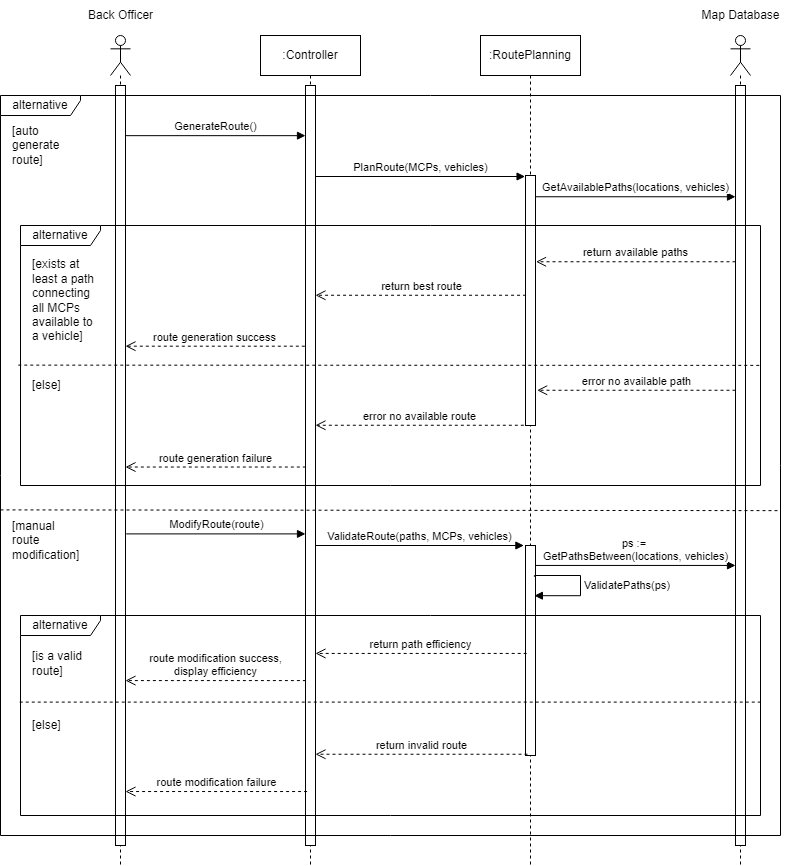
\includegraphics[width=1\linewidth]{imgs/sequence diagram/Sequence Diagram 2.2.png}
            \caption{Sequence diagram cho Task Route Planning}
        \end{figure}
    
        \newpage

\section{Class Diagram cho task assignment module}
     \begin{figure}[h]
        \centering
        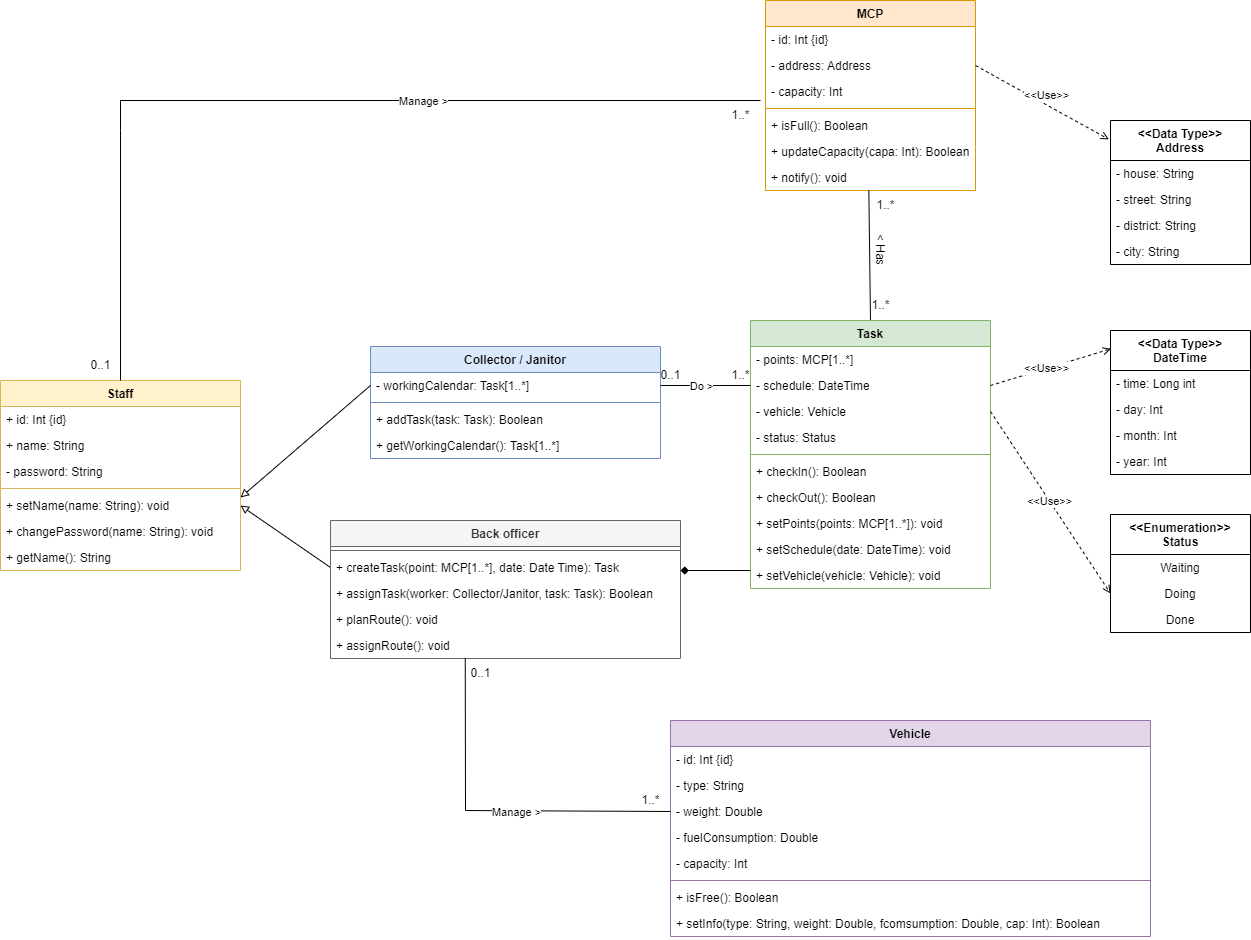
\includegraphics[width=15cm,height=15cm]{imgs/class diagram/class diagram.png}
        \caption{Class diagram cho task assignment module}
    \end{figure}

    \newpage
    -Có tất cả 6 class trong module trên gồm có:
    \begin{enumerate}
        \item Class Staff:
        \begin{table}[htp]
            \begin{tabular}{|lll|}
                \hline
                \multicolumn{1}{|l|}{Class Name} & \multicolumn{2}{l|}{Staff}                                     \\ \hline
                \multicolumn{1}{|l|}{Inherit}    & \multicolumn{2}{l|}{None}                                      \\ \hline
                \multicolumn{3}{|c|}{\cellcolor[HTML]{FFFFC7}Attributes}                                          \\ \hline
                \multicolumn{1}{|l|}{int}        & \multicolumn{1}{l|}{id}               & Số định danh nhân viên \\ \hline
                \multicolumn{1}{|l|}{string}     & \multicolumn{1}{l|}{name}             & Tên nhân viên          \\ \hline
                \multicolumn{1}{|l|}{string}     & \multicolumn{1}{l|}{password}         & Mật khẩu đăng nhập     \\ \hline
                \multicolumn{3}{|c|}{\cellcolor[HTML]{FFFFC7}Methods}                                             \\ \hline
                \multicolumn{1}{|l|}{void}       & \multicolumn{1}{l|}{setName()}        & Đặt tên cho nhân viên  \\ \hline
                \multicolumn{1}{|l|}{void}       & \multicolumn{1}{l|}{changePassword()} & Đổi mật khẩu           \\ \hline
                \multicolumn{1}{|l|}{string}     & \multicolumn{1}{l|}{getName()}        & Lấy tên nhân viên      \\ \hline
                \multicolumn{3}{|c|}{\cellcolor[HTML]{FFFFC7}Relationships}                                       \\ \hline
                \multicolumn{1}{|l|}{Manage}     & \multicolumn{2}{l|}{Quản lý thông tin các MCP}                 \\ \hline
            \end{tabular}
        \end{table}
                
        \item Class Collector / Janitor:
        \begin{table}[htp]
            \begin{tabular}{|lll|}
                \hline
                \multicolumn{1}{|l|}{Class Name} & \multicolumn{2}{l|}{Collector/Janitor}                              \\ \hline
                \multicolumn{1}{|l|}{Inherit}    & \multicolumn{2}{l|}{Staff}                                          \\ \hline
                \multicolumn{3}{|c|}{\cellcolor[HTML]{FFFFC7}Attributes}                                               \\ \hline
                \multicolumn{1}{|l|}{Task{[}{]}} & \multicolumn{1}{l|}{workingCalendar}      & Lịch làm việc           \\ \hline
                \multicolumn{3}{|c|}{\cellcolor[HTML]{FFFFC7}Methods}                                                  \\ \hline
                \multicolumn{1}{|l|}{boolean}    & \multicolumn{1}{l|}{addTask()}            & Thêm task vào phần lịch \\ \hline
                \multicolumn{1}{|l|}{Task{[}{]}} & \multicolumn{1}{l|}{getWorkingCalendar()} & Lấy, xem lịch làm việc  \\ \hline
                \multicolumn{3}{|c|}{\cellcolor[HTML]{FFFFC7}Relationships}                                            \\ \hline
                \multicolumn{1}{|l|}{Do}         & \multicolumn{2}{l|}{Collector và Janitor thực hiện task}            \\ \hline
            \end{tabular}
        \end{table}
            
        \item Class Back officer:
        \begin{table}[htp]
            \begin{tabular}{|lll|}
                \hline
                \multicolumn{1}{|l|}{Class Name}  & \multicolumn{2}{l|}{Back officer}                                     \\ \hline
                \multicolumn{1}{|l|}{Inherit}     & \multicolumn{2}{l|}{Staff}                                            \\ \hline
                \multicolumn{3}{|c|}{\cellcolor[HTML]{FFFFC7}Attributes}                                                  \\ \hline
                \multicolumn{3}{|c|}{\cellcolor[HTML]{FFFFC7}Methods}                                                     \\ \hline
                \multicolumn{1}{|l|}{Task}        & \multicolumn{1}{l|}{createTask()} & Tạo task                          \\ \hline
                \multicolumn{1}{|l|}{boolean}     & \multicolumn{1}{l|}{assignTask()} & Gán task cho collector và janitor \\ \hline
                \multicolumn{1}{|l|}{void}        & \multicolumn{1}{l|}{planRoute()}  & Tạo tuyến đường                   \\ \hline
                \multicolumn{3}{|c|}{\cellcolor[HTML]{FFFFC7}Relationships}                                               \\ \hline
                \multicolumn{1}{|l|}{Manage}      & \multicolumn{2}{l|}{Quản lý thông tin phương tiện}                    \\ \hline
                \multicolumn{1}{|l|}{Composition} & \multicolumn{2}{l|}{Bao gồm task}                                     \\ \hline
            \end{tabular}
        \end{table}
    
        \newpage
            
        \item Class Task:
        \begin{table}[htp]
            \begin{tabular}{|lll|}
                \hline
                \multicolumn{1}{|l|}{Class Name} & \multicolumn{2}{l|}{Task}                                          \\ \hline
                \multicolumn{1}{|l|}{Inherit}    & \multicolumn{2}{l|}{None}                                          \\ \hline
                \multicolumn{3}{|c|}{\cellcolor[HTML]{FFFFC7}Attributes}                                              \\ \hline
                \multicolumn{1}{|l|}{MCP{[}{]}}  & \multicolumn{1}{l|}{points}        & Danh sách các MCP của task    \\ \hline
                \multicolumn{1}{|l|}{DateTime}   & \multicolumn{1}{l|}{schedule}      & Thời gian làm cho task        \\ \hline
                \multicolumn{1}{|l|}{Vehicle}    & \multicolumn{1}{l|}{vehicle}       & Phương tiện dùng cho task     \\ \hline
                \multicolumn{1}{|l|}{Status}     & \multicolumn{1}{l|}{status}        & Trạng thái của task           \\ \hline
                \multicolumn{3}{|c|}{\cellcolor[HTML]{FFFFC7}Methods}                                                 \\ \hline
                \multicolumn{1}{|l|}{boolean}    & \multicolumn{1}{l|}{checkIn()}     & check in task                 \\ \hline
                \multicolumn{1}{|l|}{boolean}    & \multicolumn{1}{l|}{checkOut()}    & check out task                \\ \hline
                \multicolumn{1}{|l|}{void}       & \multicolumn{1}{l|}{setPoints()}   & Đặt danh sách MCP cho task    \\ \hline
                \multicolumn{1}{|l|}{void}       & \multicolumn{1}{l|}{setSchedule()} & Đặt lịch cho task             \\ \hline
                \multicolumn{1}{|l|}{void}       & \multicolumn{1}{l|}{setVehicle()}  & Đặt phương tiện dùng cho task \\ \hline
                \multicolumn{3}{|c|}{\cellcolor[HTML]{FFFFC7}Relationships}                                           \\ \hline
                \multicolumn{1}{|l|}{Has}        & \multicolumn{2}{l|}{Mang thông tin các MCP}                        \\ \hline
            \end{tabular}
        \end{table}
            
            
        \item Class Vehicle:
        \begin{table}[htp]
            \begin{tabular}{|lll|}
                \hline
                \multicolumn{1}{|l|}{Class Name} & \multicolumn{2}{l|}{Vehicle}                                                               \\ \hline
                \multicolumn{1}{|l|}{Inherit}    & \multicolumn{2}{l|}{None}                                                                  \\ \hline
                \multicolumn{3}{|c|}{\cellcolor[HTML]{FFFFC7}Attributes}                                                                      \\ \hline
                \multicolumn{1}{|l|}{int}        & \multicolumn{1}{l|}{id}              & Số định danh phương tiện                            \\ \hline
                \multicolumn{1}{|l|}{string}     & \multicolumn{1}{l|}{type}            & Loại phương tiện                                    \\ \hline
                \multicolumn{1}{|l|}{double}     & \multicolumn{1}{l|}{weight}          & Khối lượng phương tiện                              \\ \hline
                \multicolumn{1}{|l|}{double}     & \multicolumn{1}{l|}{fuelConsumption} & Mức tiêu thụ nhiên liệu                             \\ \hline
                \multicolumn{1}{|l|}{int}        & \multicolumn{1}{l|}{capacity}        & Sức chứa của phương tiện                            \\ \hline
                \multicolumn{3}{|c|}{\cellcolor[HTML]{FFFFC7}Methods}                                                                         \\ \hline
                \multicolumn{1}{|l|}{boolean}    & \multicolumn{1}{l|}{isFree()}        & Kiểm tra phương tiện có đang được sử dụng hay không \\ \hline
                \multicolumn{1}{|l|}{boolean}    & \multicolumn{1}{l|}{setInfo()}       & Đặt thông tin cho phương tiện                       \\ \hline
                \multicolumn{3}{|c|}{\cellcolor[HTML]{FFFFC7}Relationships}                                                                   \\ \hline
            \end{tabular}
        \end{table}
            
        \newpage
        \item Class MCP:
        \begin{table}[htp]
            \begin{tabular}{|lll|}
                \hline
                \multicolumn{1}{|l|}{Class Name} & \multicolumn{2}{l|}{MCP}                                                            \\ \hline
                \multicolumn{1}{|l|}{Inherit}    & \multicolumn{2}{l|}{None}                                                           \\ \hline
                \multicolumn{3}{|c|}{\cellcolor[HTML]{FFFFC7}Attributes}                                                               \\ \hline
                \multicolumn{1}{|l|}{int}        & \multicolumn{1}{l|}{id}               & Số định danh cho MCP                        \\ \hline
                \multicolumn{1}{|l|}{Address}    & \multicolumn{1}{l|}{address}          & Địa chỉ của MCP                             \\ \hline
                \multicolumn{1}{|l|}{int}        & \multicolumn{1}{l|}{capacity}         & Sức chứa của MCP                            \\ \hline
                \multicolumn{1}{|l|}{int}        & \multicolumn{1}{l|}{capacity}         & Sức chứa của phương tiện                    \\ \hline
                \multicolumn{3}{|c|}{\cellcolor[HTML]{FFFFC7}Methods}                                                                  \\ \hline
                \multicolumn{1}{|l|}{boolean}    & \multicolumn{1}{l|}{isFull()}         & Kiểm tra MCP có đang đầy chỗ chứa hay không \\ \hline
                \multicolumn{1}{|l|}{boolean}    & \multicolumn{1}{l|}{updateCapacity()} & Cập nhật lại sức chứa MCP                   \\ \hline
                \multicolumn{1}{|l|}{void}       & \multicolumn{1}{l|}{notify()}         & Thông báo khi MCP hết sức chứa              \\ \hline
                \multicolumn{3}{|c|}{\cellcolor[HTML]{FFFFC7}Relationships}                                                            \\ \hline
            \end{tabular}
        \end{table}
\end{enumerate}

	\section{Mô tả thiết kế kiến trúc để xây dựng hệ thống}
    \quad Sau khi xác định rõ bài toàn, dựa trên những yêu cầu cả về mặt chứng năng và phi chức năng, nhóm quyết định đưa ra thiết kế hệ thống như sau:

    \vspace{1cm}
    \begin{figure}[h]
    	\centering
    	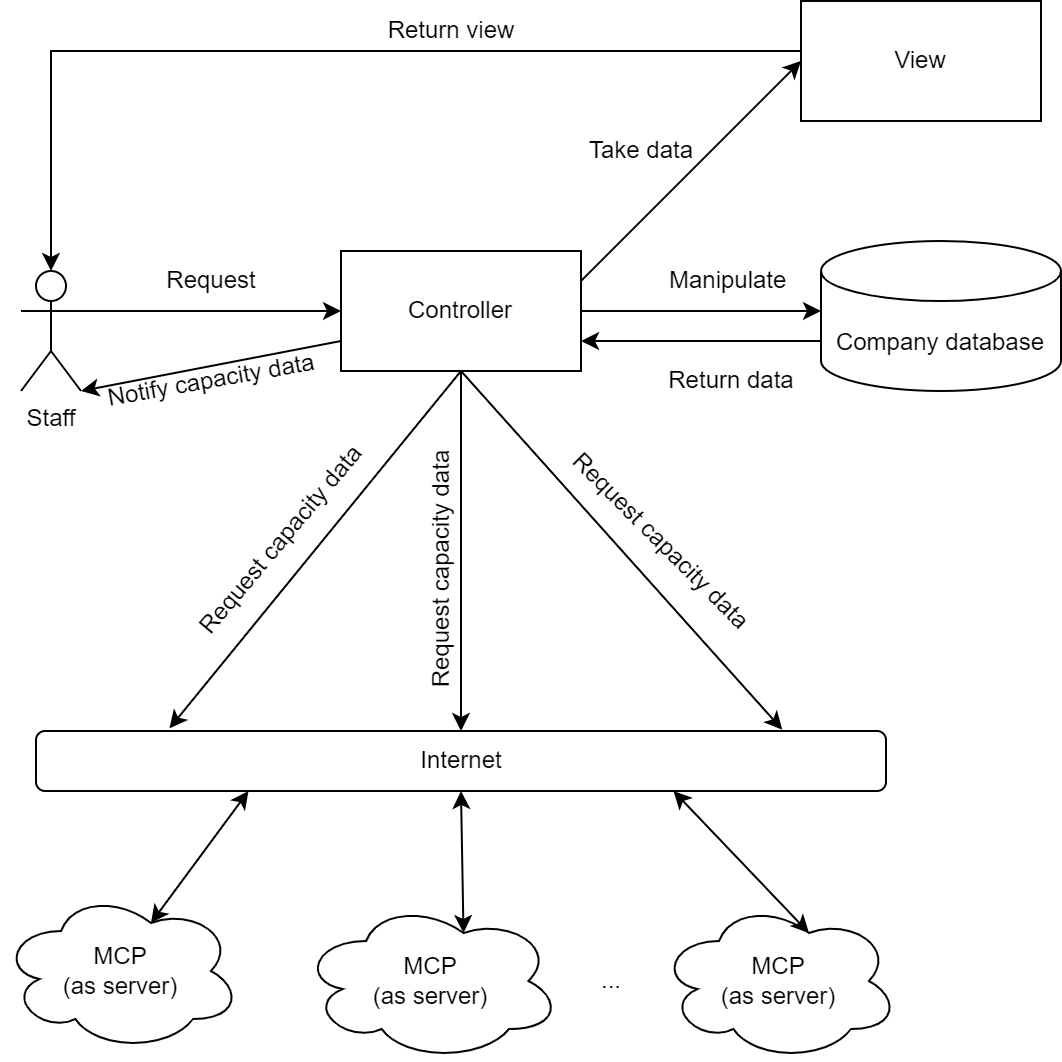
\includegraphics[width=1\linewidth]{imgs/architecture design.png}
    	\caption{Thiết kế kiến trúc của hệ thống}
    \end{figure}

   	\begin{tblr}{
   			width=1\linewidth,
   			hlines,
   			vlines,
   			colspec={X[3]X[7]},
   			columns = {valign = m, },
			column{1} = {halign = c},
   			row{1} = {halign = c, valign = m, bg = lightgray, fg = black},
   		}
   		{\textbf{Table} & \textbf{Architecture design}}  \\
   		Pattern		& 	MVC + Pub-sub \\
   		Description & 	1. Với các thông tin cơ bản như thông tin cá nhân, lịch làm, thông tin về phương tiện, ta sử dụng mô hình MVC để lấy dữ liệu và hiển thị lên cho người dùng. \newline
						\newline
		   				2. Với các thông tin về sức chứa của các MCP, ta sử dụng mô hình publisher - subscriber với Controller đóng vai trò là subscriber và MCP là các publisher. \newline
						\newline
		   				3. Với các thông báo về việc sức chứa của các MCP đạt mức tối đa ta sử dụng mô hình publisher - subscriber với Controller lúc này đóng vai trò là publisher và nhân viên là các subscriber. \\
		Flow & 			1. Controller nhận request từ người dùng -> gọi đến database thực hiện yêu cầu -> database gửi kết qua sau khi thực hiện lại cho controller -> controller gửi dữ liệu vừa nhận được cho phần View -> View hiển thị kết quả cho người dùng. \newline
						\newline
						2. Controller nhận dữ liệu từ tất cả các sensor của từng MCP sau mỗi 15 phút. Nếu sau ba lần controller không nhận được dữ liệu, sensor xem như bị mất kết nối và thực hiện thiết lập lại kết nối với sensor của MCP đó. \newline
						\newline
						3. Ngay sau khi nhận dữ liệu từ các sensor, controller thực hiện broadcast dữ liệu nếu sức chứa đã đầy đến collector/janitor liên quan đến MCP đó. \\
   	\end{tblr}

   	\vspace{0.5cm}

	\quad \textbf{Những nguyên nhân nhóm chọn kiến trúc trên:}
	\begin{enumerate}
		\item[-] MCP (Model - Controller - View) là kiểu kiến trúc bao gồm 3 chủ thể lớn là Controller - đảm nhiệm việc kiểm tra và thực hiện các yêu cầu được gửi đến, Model - đảm nhiệm việc truy suất dữ liệu của hệ thống và View - là cái được trả về cho người dùng, cái được hiển thị trên màn hình. MCP phù hợp với yêu cầu hiện thực ứng dụng trên nền tảng web, dễ dàng trong việc thiết kế, triển khai hệ thống.
		\item[-] Publisher - Subcriber cho cho phép hệ thống nhận thông tin liên tục về các điểm MCP và gửi đến người dùng những thông tin kịp thời nhất khi một hay nhiều điểm MCP bị đầy.
		\item[-] Xét tương đối với các kiến trúc khác:
		\begin{enumerate}
			\item[+] Mặc dù Layer và MCV đều được thiết kế theo kiểu module, trong đó các khối được tách ra đảm nhiệm từng chức năng riêng biệt, khi cần nâng cấp một module sẽ không ảnh hưởng đến hoạt động của các module khác. Tuy nhiên MVC có hiệu suất tốt hơn Layer, vì dữ liệu được truyền qua một tầng duy nhất, khác với việc khi truyền dữ liệu ở kiến trúc Layer phải đi qua nhiều lớp dẫn tới hao phí thời gian truyển dữ liệu từ lớp này sang lớp kia
			\item[+] Peer-to-Peer là kiểu thiết kế trong đó các client sẽ kết nối trực tiếp với nhau, trong trường hợp ứng dụng quản lý có số lượng lớn các client (bao gồm back officer, janitor, collect), việc kết nối trực tiếp các thiết bị sẽ gây ra sự chồng chéo, khó khăn trong việc kiểm soát cũng như bảo trì
			\item[+] Pipe-filter có lợi thế trong việc tách dữ liệu có độ phức tạp cao thành dữ liệu sạch thông qua các lớp màn lọc (filter), tuy nhiên hạn chế của kién trúc này là ở việc với những nguồn data khác nhau, nó sẽ yêu cầu một luồng riêng, khả năng tái sử dụng các luồng cũ rất thấp. Đối với bài toán mà nhóm đang giải quyết, việc dữ liệu mà các MCP trả về là khác nhau, nguyên nhân có thể do sự khác biệt về phần cứng hay phần mềm của các cảm biến, chính vì thế nếu sử dụng Pipe-filter thì ta phải tạo ra nhiều luồng xử lý đối với từng MCP.
		\end{enumerate}
	\end{enumerate}
  
	\newpage
   	\quad Đối với bài toán được đặt ra, ta sẽ có tổng cộng 6 module. Bao gồm:
   	\begin{enumerate}
   		\item Module Xác thực

   		\begin{tblr}{
   				width=1\linewidth,
   				hlines,
   				vlines,
   				colspec={X[3]X[7]},
   				columns = {valign = m, },
   			}
   			Input & Người dùng X \\
   			Output & Người dùng X có được truy cập hay không \newline
   					 Vai trò của người dùng X là gì \\
   			Method & Validation() \newline
   			 		 Login() \newline
   			 		 Logout() \newline
   			 		 ChangePassword() \\
   		\end{tblr}

   		\item Module Chat

  		\begin{tblr}{
  				width=1\linewidth,
  				hlines,
  				vlines,
  				colspec={X[3]X[7]},
  				columns = {valign = m, },
  			}
  			Input & Tin nhắn, văn bản\\
  			Output & Hệ thống gửi tin nhắn cho người dùng \newline
  					 Người dùng nhận được tin nhắn \\
  			Method & ConnectUser() \newline
		  			 SendMessage() \newline
		  			 NotifyMessage() \\
  		\end{tblr}

  		\item Module View information

  		\begin{tblr}{
  				width=1\linewidth,
  				hlines,
  				vlines,
  				colspec={X[3]X[7]},
  				columns = {valign = m, },
  			}
  			Input & MCP X \newline
  			Phương tiện Y \newline
  			Nhân viên Z \\
  			Output & Thông tin của MCP X \newline
  			Thông tin phương tiện Y \newline
  			Thông tin nhân viên và lịch làm của nhân viên Z \\
  			Method & ShowInfoMCP() \newline
  			ShowInfoVehicle() \newline
  			ShowInfoStaff() \newline
  			ShowDailyTask() \newline
  			ShowCalendar() \\
  		\end{tblr}
   		

   		\item Module Manage Resource

   		\begin{tblr}{
   				width=1\linewidth,
   				hlines,
   				vlines,
   				colspec={X[3]X[7]},
   				columns = {valign = m, },
   			}
   			Input & Nhân viên X, phương tiện Y\\
   			Output & Nhân viên X được chỉnh sửa \newline
   					 Phương tiện Y được chỉnh sửa \\
   			Method & AddUser() \newline
		   		     EditUser() \newline
		   			 DeactivateUser() \newline
   					 \newline
		   			 AddVehicle() \newline
		   			 EditVehicle() \newline
		   			 DeactivateVehicle() \\
   		\end{tblr}
   		
		\newpage
   		\item Module Planning route

   		\begin{tblr}{
   				width=1\linewidth,
   				hlines,
   				vlines,
   				colspec={X[3]X[7]},
   				columns = {valign = m, },
   			}
   			Input & MCP, Vehicle \\
   			Output & Tuyến đường khả dụng \\
   			Method & GenerateRoute() \newline
	   				 PlanRoute() \newline
	   				 GetAvailablePaths() \newline
	   				 ModifyRoute() \newline
	   				 ValidateRoute() \newline
	   				 GetPathsBetween() \newline
	   				 ValidatePath() \\
   		\end{tblr}

   		\item Module Task assign

   		\begin{tblr}{
   				width=1\linewidth,
   				hlines,
   				vlines,
   				colspec={X[3]X[7]},
   				columns = {valign = m, },
   			}
   			Input &	Nhân viên X \newline
   				    Công việc Y \\
   			Output & Công việc được chia thành công cho nhân viên \newline
   					 Thông báo lịch làm cho nhân viên \\
   			Method & CreateTask() \newline
   					 SetMCP() \newline
   					 SetVehicle() \newline
   					 SetSchedule() \newline
   					 AssignTask() \\
   		\end{tblr}

   	\end{enumerate}
\newpage

\section{Component Diagram cho Task Assignment Module}
    \subsection{Component Diagram Task Assignment}
         \begin{figure}[h]
            \centering
            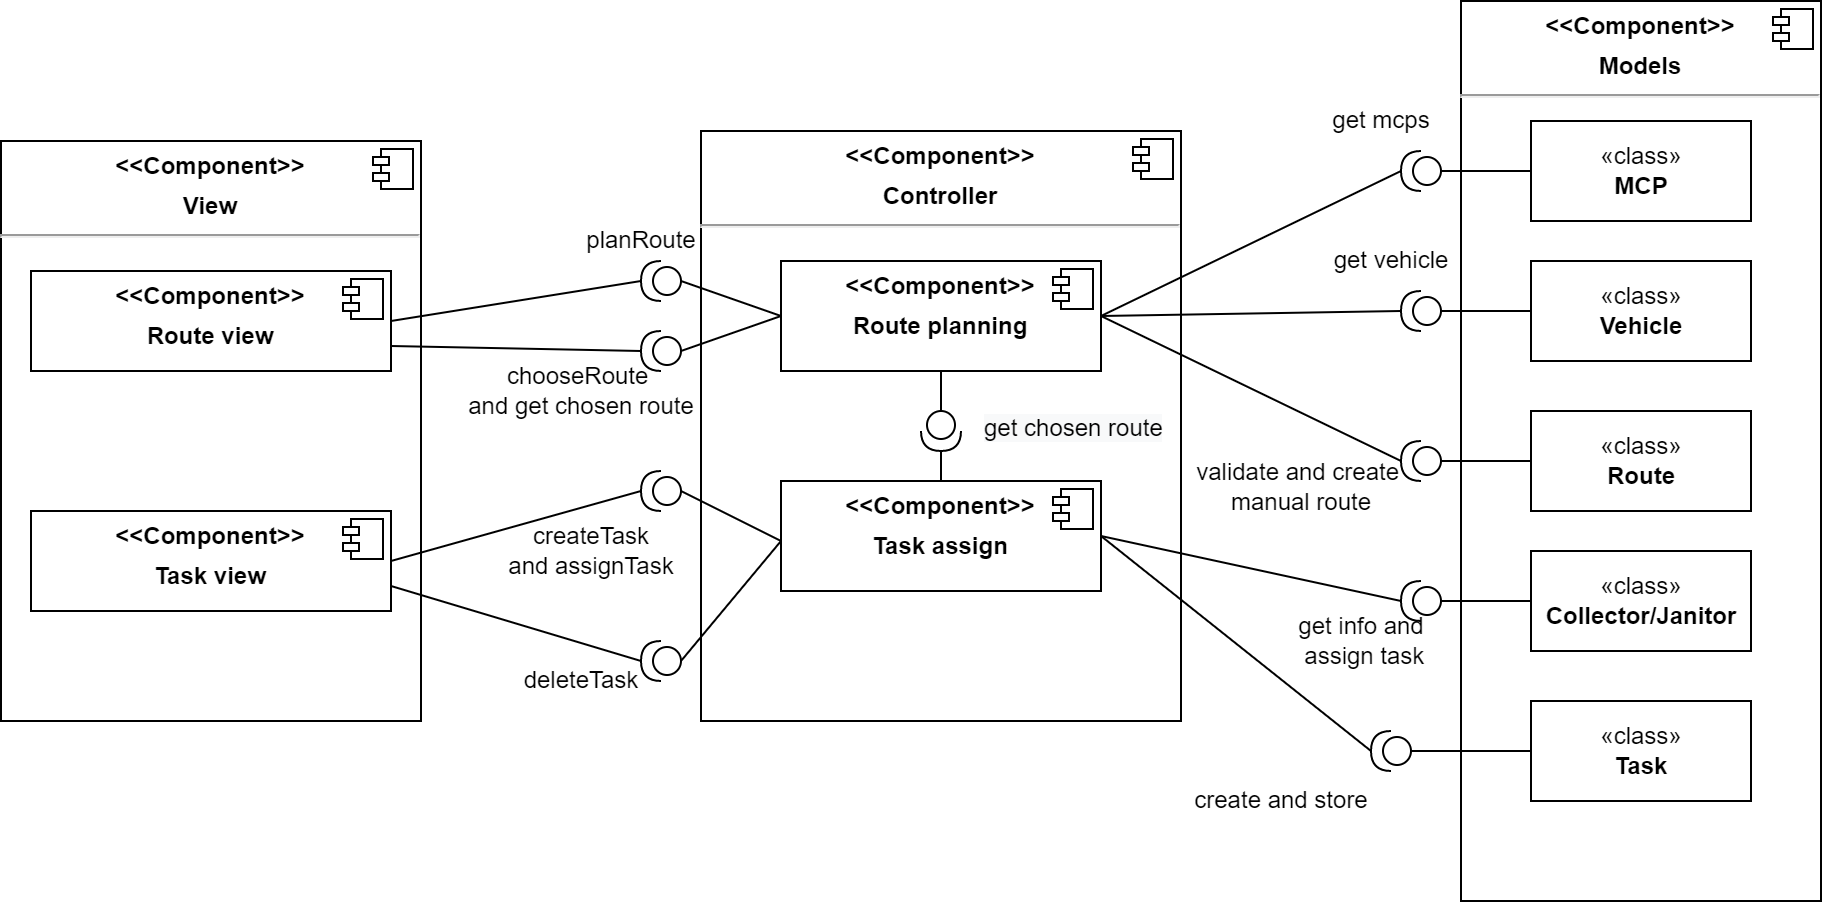
\includegraphics[width=1\linewidth]{imgs/component diagram/component Task Assignment.png}
            \caption{Component diagram cho task assignment module}
        \end{figure}
        Component diagram Task Asignment module gồm 5 Component với luồng thực thi:
        \begin{enumerate}
            \item Đưa dữ liệu Vehicle và MCPs vào Component Planning route và trả về tuyến đường khả dụng.
            \item Đưa dữ liệu các tuyến đường khả dụng vào component Choose route và trả về tuyến đường đã được Back Officer chọn.
            \item Đưa tuyến đường được chọn và Task vào Component Assign route, dữ liệu trả về là Task đã được Assign route.
            \item Đưa dữ liệu Task đã được Assign vào component Schedule time và trả về dữ liệu là Task được định thời gian thực hiện.
            \item Đưa lịch làm đã xếp và Worker vào component Assign staff và trả về kết quả là Task đã được Assign Worker, vehicle, route, calendar.
        \end{enumerate}
    \subsection{Component Diagram cho Planning Route }
        \begin{figure}[h]
            \centering
            \includegraphics[width=1\linewidth]{imgs/Component diagram/Component planning route.png}
            \caption{Component diagram cho Planning Route}
        \end{figure}
        Component diagram cho Planning Route gồm 2 Component thừa kế Component Modification Method với luồn thực thi:
        \begin{itemize}
            \item Auto generate route:
            \begin{enumerate}
                \item Đưa dữ liệu Vehicle, MCPs vào Component Get Avaiable Paths và trả về tuyến đường khả thi.
                \item Đưa dữ liệu các tuyến đường khả dụng vào Component Generate routes and Efficiency Statistic và trả về kết quả là tuyến đường hiệu quả để sử dụng.
            \end{enumerate}

            \item Manual generate route:
            \begin{enumerate}
                \item Đưa dữ liệu tuyến đường vào Component Validate Routes để kiểm thử và trả về tuyến đường đã được kiểm tra.
                \item Đưa tuyến đường đã được kiểm tra vào Component Generate routes and Efficiency Statistic và trả về kết quả là tuyến đường hiệu quả để sử dụng.
            \end{enumerate}
        \end{itemize}
       
       


\end{document}


\documentclass[a4paper]{article}
\usepackage{amssymb,epsfig,latexsym,multicol,array,hhline,fancyhdr}
\usepackage{vntex}
\usepackage{xcolor}
\usepackage{titlesec}
\usepackage{mdframed}
\usepackage{amsmath}
\usepackage{lastpage}
\usepackage[lined,boxed,commentsnumbered]{algorithm2e}
\usepackage{enumerate}
\usepackage{color}
\usepackage[most]{tcolorbox}
\usepackage{graphicx}
\usepackage{array}
\usepackage{float}
\usepackage{tabularx, caption}
\usepackage{tabularray}
\usepackage{colortbl}
\usepackage{longtable}
\usepackage{multirow} 
\usepackage{multicol}
\usepackage{rotating}
\usepackage{graphics}
\usepackage{geometry}
\usepackage{setspace}
\usepackage{epsfig}
\usepackage{wrapfig}
\usepackage{tikz}
\usepackage[most]{tcolorbox}
\usepackage{hyperref}
\usepackage{cleveref}
\usepackage{setspace}
\usepackage{subfiles}
\usepackage{indentfirst}

\hypersetup{urlcolor=blue,linkcolor=black,citecolor=black,colorlinks=true} 
\usetikzlibrary{arrows,snakes,backgrounds}

\newtheorem{theorem}{{\bf Theorem}}
\newtheorem{property}{{\bf Property}}
\newtheorem{proposition}{{\bf Proposition}}
\newtheorem{corollary}[proposition]{{\bf Corollary}}
\newtheorem{lemma}[proposition]{{\bf Lemma}}

\AtBeginDocument{\renewcommand*\contentsname{Nội dung}}
\AtBeginDocument{\renewcommand*\refname{Tham khảo}}
\setlength{\headheight}{40pt}
\pagestyle{fancy}

\fancyhead{}
\fancyhead[L]{
 \begin{tabular}{rl}
    \begin{picture}(25,15)(0,0)
    \put(0,-8){
\includegraphics[width=8mm, height=8mm]{imgs/hcmut.png}}
    %\put(0,-8){\epsfig{width=10mm,figure=hcmut.eps}}
   \end{picture}&
	%
\includegraphics[width=8mm, height=8mm]{hcmut.png} & %
	\begin{tabular}{l}
		\textbf{\bf \ttfamily Đại học Bách Khoa Thành phố Hồ Chí Minh}\\
		\textbf{\bf \ttfamily Khoa Khoa học và Kỹ thuật Máy tính}
	\end{tabular} 	
 \end{tabular}
}
\fancyhead[R]{
	\begin{tabular}{l}
		\tiny \bf \\
		\tiny \bf 
	\end{tabular} 
}
\fancyfoot{} 
\fancyfoot[L]{\scriptsize \ttfamily Bài tập lớn môn Công nghệ phần mềm - Năm học 2022-2023}
\fancyfoot[R]{\scriptsize \ttfamily Trang {\thepage}/\pageref{LastPage}}

\renewcommand{\headrulewidth}{0.3pt}
\renewcommand{\footrulewidth}{0.3pt}


%%%
\setcounter{secnumdepth}{4}
\setcounter{tocdepth}{3}
\makeatletter
\newcounter {subsubsubsection}[subsubsection]
\renewcommand\thesubsubsubsection{\thesubsubsection .\@alph\c@subsubsubsection}
\newcommand\subsubsubsection{\@startsection{subsubsubsection}{4}{\z@}%
                                     {-3.25ex\@plus -1ex \@minus -.2ex}%
                                     {1.5ex \@plus .2ex}%
                                     {\normalfont\normalsize\bfseries}}
\newcommand*\l@subsubsubsection{\@dottedtocline{3}{10.0em}{4.1em}}
\newcommand*{\subsubsubsectionmark}[1]{}
\makeatother


\begin{document}

	\begin{titlepage}
    \begin{center}
        ĐẠI HỌC QUỐC GIA THÀNH PHỐ HỒ CHÍ MINH\\
        TRƯỜNG ĐẠI HỌC BÁCH KHOA \\
        KHOA KHOA HỌC VÀ KỸ THUẬT MÁY TÍNH
    \end{center}

    \vspace{0.4cm}

    \begin{figure}[h!]
        \begin{center}
        
\includegraphics[width=4.5cm]{imgs/hcmut.png}
        \end{center}
    \end{figure}

    \vspace{0.1cm}


    \begin{center}
        \begin{tabular}{c}
        \textbf{{ \Large CÔNG NGHỆ PHẦN MỀM (CO3001)}}\\
        ~~\\
        \hline
        \\
        \multicolumn{1}{l}{\textbf{{\Large Bài tập lớn}}}\\
        \\
        \textbf{\Huge \color{red} URBAN WASTE COLLECTION}\\\\
        \textbf{\Huge \color{red} AID - UWC 2.0}\\
        \\
        \hline
        \end{tabular}
    \end{center}

    \vspace{0.5cm}

    \begin{table}[h]
        \begin{tabular}{rrl}
            \hspace{5 cm} & GVHD: & Lê Đình Thuận.\\
            & Lớp: & L04\_ Nhóm: Tình Đồng Chí \\
            & Sinh viên thực hiện: & Lê Nguyễn Huyền Thoại – 2012122.\\
            & & Trương Huy Thái – 2012036.\\
            & & Nguyễn Tiến Nam – 2011652.\\
            & & Nguyễn Trọng Đức Huy – 2011283.\\
            & & Nguyễn Trọng Nhân – 2011744.\\
            & & Trần Tuấn Anh – 2010878.\\
            & & Phan Thị Quỳnh Như – 2011780. \\
        \end{tabular}
    \end{table}

    \vspace{0.3CM}

    \begin{center}
        {\footnotesize THÀNH PHỐ HỒ CHÍ MINH, THÁNG \the\month /\the\year}
    \end{center}
\end{titlepage}


	\newpage
	\tableofcontents

	\newpage
	\section{Danh sách thành viên \& Khối lượng công việc}

\begin{tblr}{
    width=1\linewidth,
    hlines,
    vlines,
    colspec={X[-2]X[4]X[1.5]X[6]X[-1]},
    columns = {valign = m, },
    column{1} = {halign = c, },
    row{1} = {halign = c, valign = m, bg = lightgray, fg = black},
}
    {\textbf{STT} & \textbf{Họ và tên} & \textbf{MSSV} & \textbf{Công việc} & \textbf{Hoàn thành} }  \\
    1 & Lê Nguyễn Huyền Thoại & 2012122 & - Quản lý tiến độ công việc \newline
                                          - Thiểt kế use-case diagram tổng \newline
                                          - Thiệt kế class diagram \newline
                                          - Thiết kế component diagram
                                        & 100\% \\
    2 & Trương Huy Thái       & 2012036 & - Xác định yêu cầu phi chức năng \newline
                                          - Thiết kế use-case diagram task assignment \newline
                                          - Thiết kế activity diagram  \newline
                                          - Thiết kế architecture design
                                        & 100\% \\
    3 & Nguyễn Tiến Nam		  & 2011652 & - Xác định yêu cầu chức năng \newline
                                          - Viết đặc tả use-case tổng \newline
                                          - Thiết kế class diagram \newline
                                          - Thiết kế architecture design
                                        & 100\% \\
    4 & Nguyễn Trọng Đức Huy  & 2011283 & - Xác định ngữ cảnh dự án \newline
                                          - Thiết kế use-case manage resources \newline
                                          - Thiết kế sequence diagram \newline
                                          - Đánh giá Architecture design
                                        & 100\% \\
    5 & Nguyễn Trọng Nhân     & 2011744 & - Xác định ngữ cảnh dự án \newline
                                          - Viết đặc tả use-case task assignment \newline
                                          - Thiết kế sequence diagram \newline
                                          - Thiết kế component diagram
                                        & 100\% \\
    6 & Trần Tuấn Anh         & 2010878 & - Xác định yêu cầu phi chức năng \newline
                                          - Đánh giá các use-case diagram \newline
                                          - Thiết kế activity diagram \newline
                                          - Đánh giá component diagram
                                        & 100\% \\
    7 & Phan Thị Quỳnh Như    & 2011780 & - Xác định yêu cầu chức năng \newline
                                          - Đánh giá activity diagram, sequence diagram, class diagram \newline
                                          - Đánh giá tổng quan task 3 \newline
                                          - Viết báo cáo
                                        & 100\% \\

\end{tblr}


	%%%%%%%%%%%%%%%%%%%%%%%%%%%%%%%%%


	%%%%%%%%%%%%%%%%%%%%%%%%%%%%%%%%%
	\newpage
	\subsection{Mô tả chung}
    \quad Sau đại dịch covid-19, sức khỏe đã và đang là một trong những vấn đề được nhiều người quan tâm. Nhận thấy được vấn đề này, nhóm muốn tạo ra một ứng dụng nhằm nâng cao sức khỏe của người sử dụng bằng việc đưa ra những món ăn phù hợp với mục tiêu nhu cầu của từng người. Ví dụ như người dùng muốn tăng cân, tăng cơ, phần mềm sẽ đưa ra các món ăn làm sao để trong một khoảng thời gian nhất định, người dùng có thể đạt được cân nặng mà họ mong muốn. Ngoài ra nó còn cung cấp cho người dùng một lượng lớn các công thức nấu ăn đơn giản mà vẫn ngon miệng, phù hợp với cuộc sống ngày càng nhanh hiện nay.\\
    
    \begin{figure}[h]
        \centering
        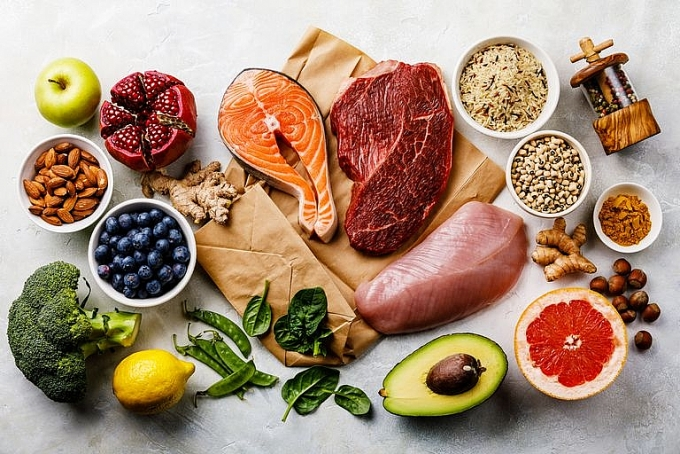
\includegraphics[width=0.7\linewidth]{images/healthy-food.jpg}
        \caption{Các chất có trong bữa ăn}
    \end{figure}
\section{Xác định ngữ cảnh của dự án UWC 2.0}
    \subsection{Các bên liên quan (Relevant Stakeholders)}
        \begin{enumerate}
            \item Công ty cung cấp dịch vụ thu dọn rác Y, ở vai trò là người quản lý.
            \item Công ty cung cấp dịch vụ thu dọn rác Y, ở vị trí là người sở hữu phần mềm UWC 2.0.
            \item Tổ chức X, phát triển phần mềm UWC 2.0.
            \item Công nhân sử dụng phần mềm UWC 2.0.
            \item Các bên liên quan khác (chính phủ, người dân).
        \end{enumerate}
    
    \subsection{Những mong muốn của các bên liên quan}
        \begin{enumerate}
            \item Công ty cung cấp dịch vụ thu dọn rác Y, ở vai trò là người quản lý, họ mong muốn phần mềm UWC 2.0 sẽ mang lại cho công ty:
            \begin{itemize}
                \item[-] Khả năng quản lý nhân lực, kiểm tra một cách hiệu quả cũng như thường xuyên cập nhật thông tin về sức chứa của các điểm tập trung rác thải (MCPs) và những thông tin nhằm phục vụ nhu cầu bảo trì các phương tiện vận chuyển, trang thiết bị của công ty.
                \item[-] Nâng cao hiệu suất thu gom rác thải của công ty.
                \item[-] Hệ thống khi được đưa vào hoạt động có độ tin cậy cao, hoạt động tốt trong mọi tình huống.
            \end{itemize}
            
            \item Công ty cung cấp dịch vụ thu dọn rác Y, ở vị trí là người sở hữu phần mềm UWC 2.0, họ sẽ có những mong muốn:
            \begin{itemize}
                \item[-] Khả năng mở rộng phạm vi hoạt động của hệ thống, không chỉ là trong một vùng, một quận cố định, mà có thể xử lý trong phạm vi toàn thành phố.
                \item[-] Chi phí và lợi nhuận luôn là một trong những vấn đề ưu tiên hàng đầu cần phải được cân nhắc. Khi được đưa vào sử dụng, UWC 2.0 phải đảm bảo tối ưu hóa về mặt nhiên liệu để từ đó giảm thiểu được chi phí phải bỏ ra. Thêm vào đó là chi phí để bảo trì hệ thống cũng phải phù hợp với công ty.
                \item[-] Trước đây công ty đã có sẵn hệ thống UWC 1.0 và công ty mong muốn có thể tận dụng lại tối đa dữ liệu có sẵn từ phiên bản trước và khả năng tương thích ngược giữa phiên bản 1.0 và 2.0.
                \item[-] Đem lại những kết quả tích cực đến công tác xử lý và tái chế rác thải trong cộng đồng, tạo ra môi trường sống xanh, sạch, đẹp cho người dân.
            \end{itemize}
      
            \item Tổ chức X, phát triển phần mềm UWC 2.0 có mong muốn:
            \begin{itemize}
                \item[-] Xây dựng được hệ thống có thể làm được và làm tốt những yêu cầu tối thiểu được yêu cầu bởi công ty chủ quản, xa hơn nữa là hoàn thiện hệ thống một cách tối ưu.
                \item[-] Hệ thống khi đến tay khách hàng phải dễ dàng bảo dưỡng, để nếu trong tương lai nếu khách hàng có thuê một công ty khác sửa chữa, bảo dưỡng hệ thống cũng thuận tiện hơn.
            \end{itemize}
        
            \item Công nhân sử dụng phần mềm UWC 2.0 mong muốn:
            \begin{itemize}
                \item[-] Vì đa phần người dùng là các cô chú trung niên, lớn tuổi, phần mềm nên có giao diện thân thiện, dễ dàng tiếp cận và làm quen.
                \item[-] Có thể sử dụng phần mềm trên nhiều thiết bị khác nhau như máy tính, điện thoại hay máy tính bảng.
                \item[-] Phần mềm phải sử dụng ổn định, ít giật lag và độ tin cậy cao.
            \end{itemize}
       
            \item Các bên liên quan khác (chính phủ, người dân): mong muốn phần mềm sẽ mang lại những ảnh hưởng tích cực đến công tác quản lý và tái sử dụng rác thải trong phạm vi khu vực và trong cả nước.
        \end{enumerate}
    
    \subsection{Vấn đề các bên liên quan đang gặp phải}
        \begin{enumerate}
            \item Công ty cung cấp dịch vụ thu dọn rác Y hiện đang gặp phải các vấn đề:
            \begin{itemize}
                \item[-] Công ty đang thiếu khả năng kiểm tra tình trạng trang thiết bị và phương tiện nên việc hoạt động chưa hiệu quả.
                \\
                \emph{\underline{Ví dụ}}: Chưa kiểm soát được tải trọng, sức chứa, tiêu thụ nhiên liệu dẫn tới sự phân bố xe chưa hợp lý khi hoạt động.
                
                \item[-] Việc quản lý nhân lực của công ty chưa hiệu quả:
                \begin{itemize}
                    \item[+] Công ty chưa theo dõi được tiến độ làm việc, hiệu suất làm việc của nhân viên.
                    \item[+] Việc phân công công việc chưa hợp lý gây mất công bằng và giảm hiệu suất công việc.
                \end{itemize}
            \end{itemize}
            
            \item Công ty cung cấp dịch vụ thu dọn rác Y, ở vị trí là người sở hữu hệ thống đang gặp phải các vấn đề:
            \begin{itemize}
                \item[-] Khả năng duy trì và nâng cấp hệ thống. Việc duy trì hệ thống đang có chi phí cao, chưa hợp lý.
                \item[-] Khi gặp các sự cố bất ngờ như  tai nạn, hư hỏng thiết bị thì việc liên lạc để điều phối nhân viên chưa kịp thời .
                \item[-] Công ty gặp bất tiện trong việc theo dõi và phân công lịch trình: lịch trình giấy, phân công thủ công. Điều này khiến công ty mất nhiều thời gian, nhân sự và việc phân công này chưa được tối ưu.
            \end{itemize}
            
            \item Các bên liên quan khác (chính phủ, người dân): Việc cải thiện môi trường chưa được tối ưu hoá, chi phí cao nhưng chưa hiệu quả dẫn đến lãng phí.
        \end{enumerate}
    
    \subsection{Lợi ích mà các bên liên quan có thể đạt được khi sử dụng hệ thống UWC 2.0}
        \begin{enumerate}
            \item Nhà cung cấp dịch vụ thu dọn rác Y ở vai trò quản lý:
            \begin{itemize}
                \item[-] Nắm bắt được cụ thể tình trạng hiện tại của các trang thiết bị và cơ sở vật chất, từ đó có thể đưa ra được những quyết định như nâng cấp, sửa chữa hay bổ sung trang thiết bị cho công nhân một cách kịp thời và hiệu quả.
                \item[-] Nhanh chóng theo dõi được tiến độ, hiệu suất làm việc của nhân viên. Đưa ra được phương án giải quyết sự cố kịp thời và công bằng.
            \end{itemize}
    
            \item Nhà cung cấp dịch vụ Y dưới góc độ chủ sở hữu hệ thống:
            \begin{itemize}
                \item[-] Tiết kiệm được chi phí duy trì và phát triển hệ thống.
                \item[-] Mang lại danh tiếng cho công ty trong mảng thu dọn rác thải.
            \end{itemize}
    
            \item Tổ chức X qua vai trò nhà phát triển phần mềm:
            \begin{itemize}
                \item[-] Tăng thu nhập cho công ty cũng như thu nhập của các cá nhân tham gia phát triển hệ thống.
                \item[-] Tăng kỹ năng của từng cá nhân.
                \item[-] Nâng cao danh tiếng, sự tin cậy cho doanh nghiệp.
            \end{itemize}
          
            \item Nhân viên  sử dụng phần mềm:
            \begin{itemize}
                \item[-] Dễ dàng sử dụng và làm quen.
                \item[-] Công sức làm việc của bản thân mỗi người được đánh giá công bằng và rõ ràng.
                \item[-] Khả năng liên lạc nhanh chóng giữa công nhân và nhân viên giám sát nhằm xử lý được những tình huống bất ngờ có thể xảy ra trong quá trình làm việc.
            \end{itemize}
            
            \item Người bị ảnh hưởng khác (chính phủ, người dân): Bảo vệ môi trường.
        \end{enumerate}
    \newpage

\section{Yêu cầu (Requirements)}
    \subsection{Yêu cầu chức năng (Functional)}
        \begin{enumerate}
            \item \textbf{Nhân viên giám sát (Back officer)}
           
            \begin{tblr}{
                width=1\linewidth,
                hlines,
                vlines,
                colspec={X[-1]X[4]X[7]},
                columns = {valign = m, },
                row{1} = {halign = c, valign = m, bg = lightgray, fg = black},
            }
                {\textbf{\#}} & \textbf{Chức năng} & {\textbf{Mô tả}} \\
                1 & Xem thông tin cá nhân & Cho phép xem chi tiết thông tin cá nhân của công nhân.\\
                2 & Xem lịch làm việc &  Xem lịch làm của từng công nhân.\\
                3 & Xem phương tiện & Xem được thông tin của từng phương tiện, các thông số kỹ thuật như trọng lượng, lượng nhiên liệu tiêu thụ, tình trạng, ...\\
                4 & Xem các điểm MCPs & Xem được thông tin các điểm MCPs, dung tích còn lại của nó.\\
                5 & Phân công công việc & Nhân viên giám sát có thể phân công công việc cho từng công nhân bao gồm việc phân phương tiện, gán các điểm MCPs và tạo tuyến đường cho công nhân lái xe rác.\\
                6 & Nhắn tin & Nhân viên giám sát có thể liên lạc với công nhân trong trường hợp bất ngờ xảy ra.\\
                7 & Thay đổi mật khẩu & Cho phép thay đổi mật khẩu trong trường hợp mong muốn hoặc thay đổi mật khẩu và có phương án xác thực dự phòng trong trường hợp quên mật khẩu.\\
                8 & Đăng nhập & Nhân viên giám sát đăng nhập vào tài khoản để sử dụng các tính năng.\\
            \end{tblr}
         
            \item \textbf{Người quản lý (Administrator)}
           
            \begin{tblr}{
                width=1\linewidth,
                hlines,
                vlines,
                colspec={X[-1]X[4]X[7]},
                columns = {valign = m, },
                row{1} = {halign = c, valign = m, bg = lightgray, fg = black},
            }
                {\textbf{\#}} & \textbf{Chức năng} & {\textbf{Mô tả}} \\
                1 & Quản lý nhân viên & Cho phép tạo, sửa, xóa một nhân viên trong hệ thống.\\
                2 & Quản lý phương tiện & Cho phép thêm, sửa, xóa một phương tiện trong hệ thống.\\
                3 & Quản lý các MCPs & Cho phép thêm, sửa, xóa các MCPs.\\
                4 & Thay đổi mật khẩu & Cho phép thay đổi mật khẩu trong trường hợp mong muốn hoặc thay đổi mật khẩu và có phương án xác thực dự phòng trong trường hợp quên mật khẩu.\\
                5 & Đăng nhập & Quản lý đăng nhập vào tài khoản để sử dụng các tính năng.\\
            \end{tblr}
           
            \newpage
            \item \textbf{Công nhân (Janitor / Collector)}
           
            \begin{tblr}{
                width=1\linewidth,
                hlines,
                vlines,
                colspec={X[-1]X[4]X[7]},
                columns = {valign = m, },
                row{1} = {halign = c, valign = m, bg = lightgray, fg = black},
            }
                {\textbf{\#}} & \textbf{Chức năng} & {\textbf{Mô tả}} \\
                1 & Xem thông tin cá nhân & Cho phép xem chi tiết thông tin cá nhân của công nhân.\\
                2 & Xem lịch làm việc & Cho phép công nhân xem lịch làm việc cụ thể trong từng ngày và tổng quát ở mỗi tuần.\\
                3 & Check in / check out & Công nhân xác nhận công việc trong ngày và đánh dấu hoàn thành công việc mỗi ngày.\\
                4 & Nhắn tin & Công nhân có thể liên lạc với văn phòng trong trường hợp bất ngờ xảy ra.\\
                5 & Nhận thông báo & Nhận thông báo mỗi khi lịch làm việc được giao cũng như tình trạng của MCPs. \\
                6 & Thay đổi mật khẩu & Cho phép thay đổi mật khẩu trong trường hợp mong muốn hoặc thay đổi mật khẩu và có phương án xác thực dự phòng trong trường hợp quên mật khẩu.\\
                7 & Đăng nhập & Công nhân đăng nhập vào tài khoản để sử dụng các tính năng.\\
            \end{tblr}
        \end{enumerate}
   
    \subsection{Yêu cầu phi chức năng (Non-functional)}
        \begin{enumerate}
            \item \textbf{Thiết kế giao diện người dùng (UI design)}
           
            \begin{tblr}{
                width=1\linewidth,
                hlines,
                vlines,
                colspec={X[-1]X[11]},
                columns = {valign = m, },
                row{1} = {halign = c, valign = m, bg = lightgray, fg = black},
            }
                {\textbf{\#}} & \textbf{Yêu cầu} \\
                1 & Thông tin quan trọng nên được hiển thị trong một lần xem (không cần kéo xuống). \\
                2 & Giao diện đơn giản. Có thể tự tìm hiểu cách sử dụng không cần hướng dẫn trong 15 phút. \\
                3 & Giao diện hệ thống: tiếng Việt và tiếng Anh cho tương lai.\\
            \end{tblr}
           
            \item \textbf{Hiệu suất (Performance)}
           
            \begin{tblr}{
                width=1\linewidth,
                hlines,
                vlines,
                colspec={X[-1]X[11]},
                columns = {valign = m, },
                row{1} = {halign = c, valign = m, bg = lightgray, fg = black},
            }
                {\textbf{\#}} & \textbf{Yêu cầu} \\
                1 & Xử lý thời gian thực với ít nhất 1000 MCPs trong thời điểm hiện tại và 10000 MCPs trong 5 năm tới.\\
                2 & Sức chứa của MCPs cần được cập nhật mỗi 15 phút. \\
                3 & Độ trễ giao tiếp thời gian thực ở dưới 1 giây. \\
                4 & Thời gian gợi ý tuyến đường tối ưu dưới 10 giây. \\
                5 & Thời gian lấy dữ liệu của công nhân dưới 5 giây. \\
            \end{tblr}
           
            \newpage
            \item \textbf{Tương thích (Compatibility)}
           
            \begin{tblr}{
                width=1\linewidth,
                hlines,
                vlines,
                colspec={X[-1]X[11]},
                columns = {valign = m, },
                row{1} = {halign = c, valign = m, bg = lightgray, fg = black},
            }
                {\textbf{\#}} & \textbf{Yêu cầu} \\
                1 & Có thể lấy và sử dụng dữ liệu cũ từ UWC 1.0.\\
                2 & Hoạt động tương thích với UWC 1.0 \\
            \end{tblr}
           
            \item \textbf{Nền tảng (Platform)}
           
            \begin{tblr}{
                width=1\linewidth,
                hlines,
                vlines,
                colspec={X[-1]X[11]},
                columns = {valign = m, },
                row{1} = {halign = c, valign = m, bg = lightgray, fg = black},
            }
                {\textbf{\#}} & \textbf{Yêu cầu} \\
                1 & Là ứng dụng web, có thể cải tiến cho ứng dụng di động trong tương lai. \\
            \end{tblr}
        \end{enumerate}
    \newpage

\section{Use-case diagram}
    

\subsection{Tổng quát của hệ thống}
    \begin{figure}[h]
        \centering
        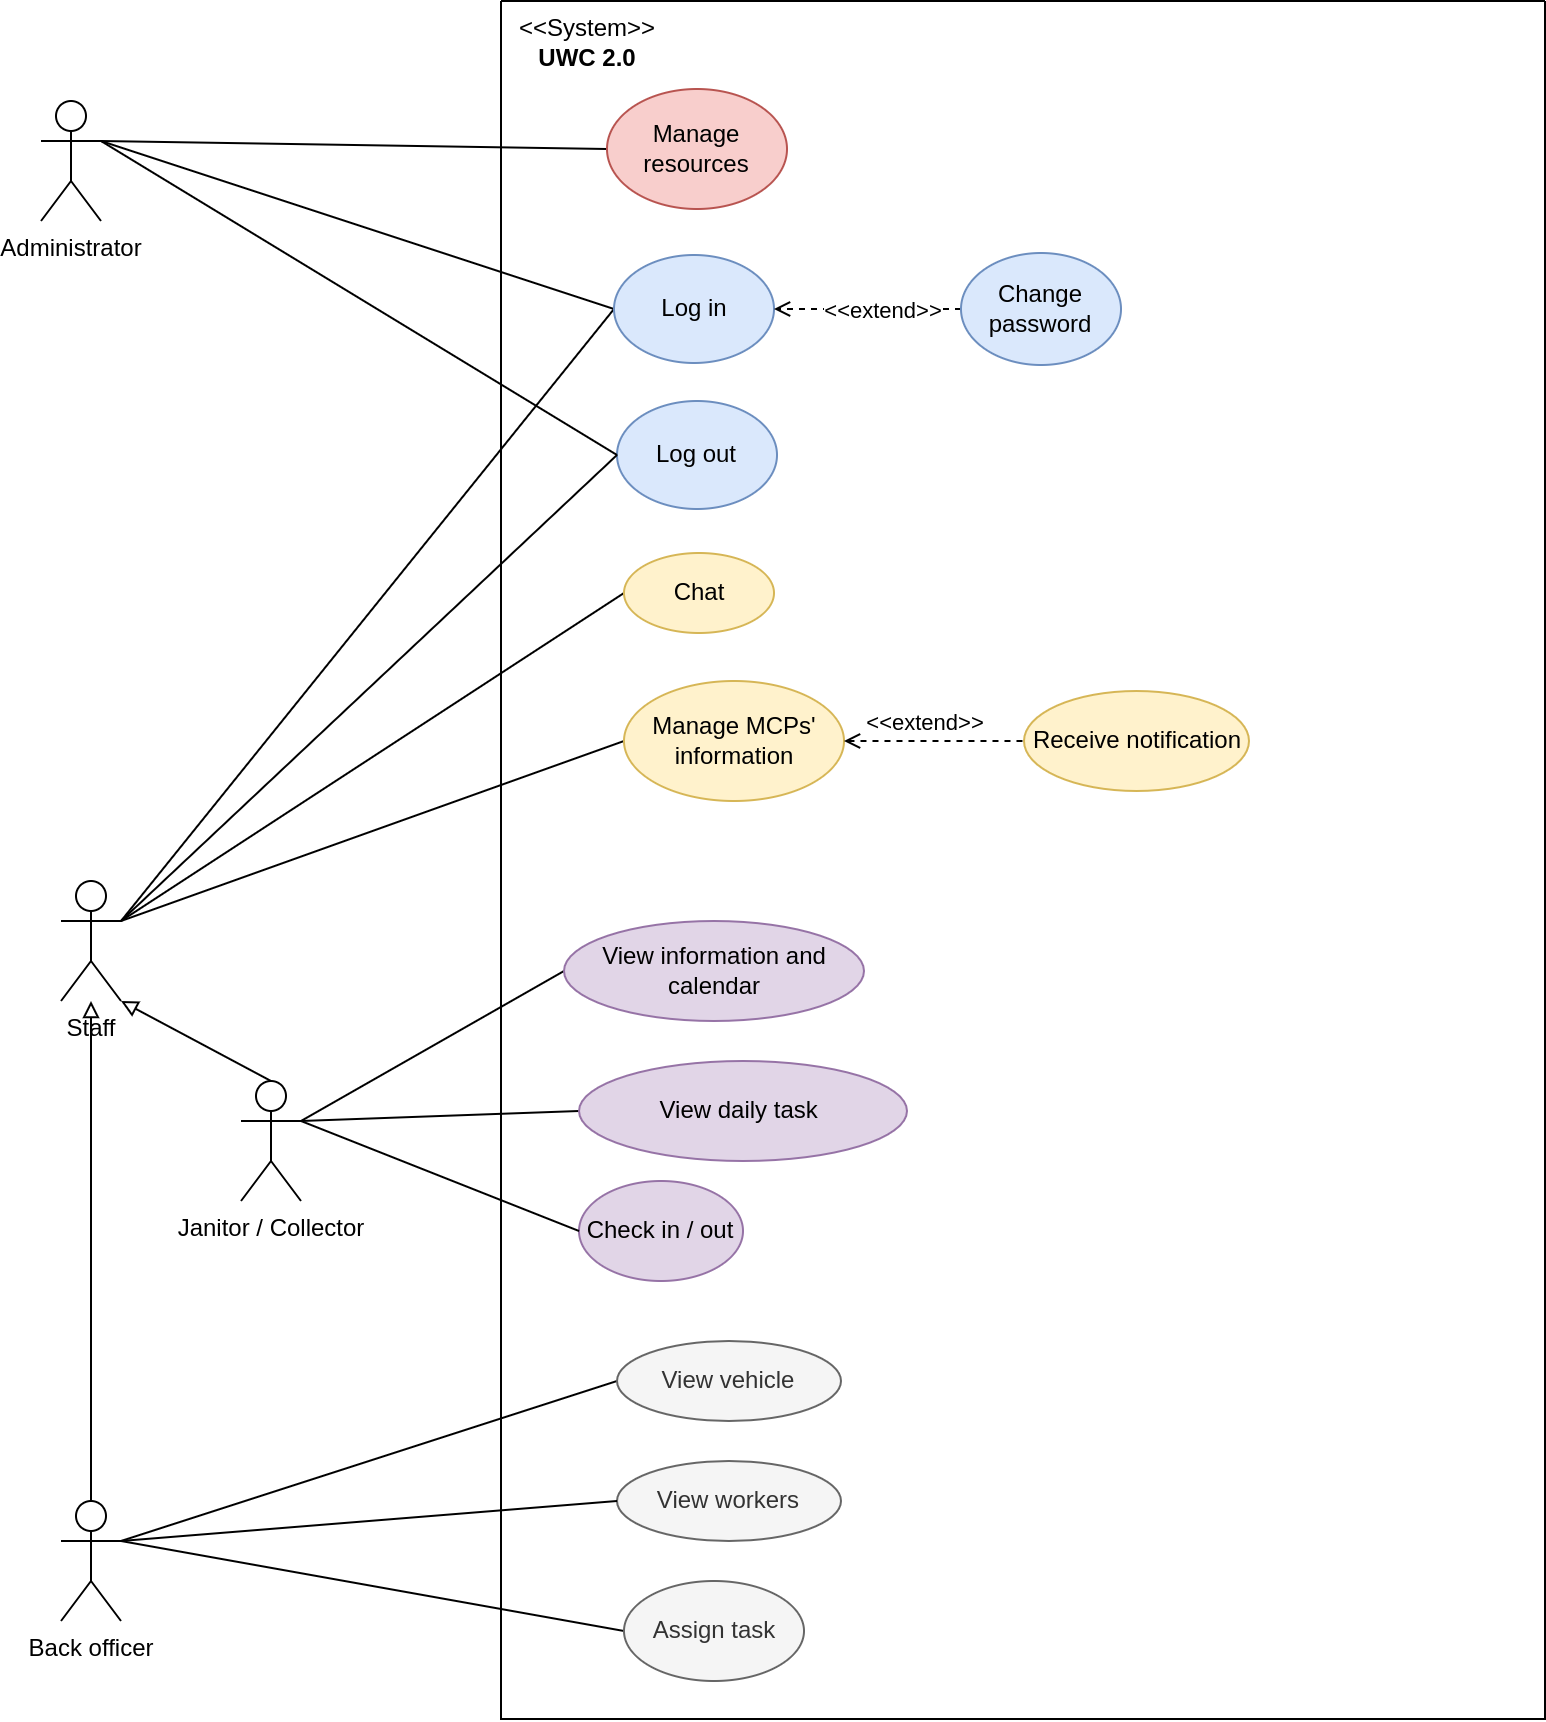
\includegraphics[width=0.93\linewidth]{imgs/use-case diagram/main_uc.png}
        \caption{Use-case diagram tổng quát của hệ thống}
    \end{figure}

    \begin{tblr}{
        width=1\linewidth,
        hlines,
        vlines,
        colspec={X[3]X[7]},
        columns = {valign = m, },
        row{1} = {halign = c, valign = m, bg = lightgray, fg = black},
    }
        {\textbf{Use case name} & \textbf{Manage resources}}  \\
        Description	& Quản lý tài nguyên của công ty \\
        Actor & Người quản lý (Administrator) \\
        Trigger & Người quản lý ấn vào phần quản lý tài nguyên  \\
        Pre-condition & Người quản lý đã đăng nhập và đang ở màn hình chính\\
        Post-condition & Người quản lý được đưa vào trang quản lý tài nguyên\\
        Normal flow &   		1. Hệ thống hiển thị giao diện quản lý tài nguyên \newline
                                2. Quản lý thực hiện việc quản lý tài nguyên \\
        Alternative flow  & 	none \\
        Exception flow & none\\
    \end{tblr}

    \vspace{1cm}

    \begin{tblr}{
        width=1\linewidth,
        hlines,
        vlines,
        colspec={X[3]X[7]},
        columns = {valign = m, },
        row{1} = {halign = c, valign = m, bg = lightgray, fg = black},
    }
        {\textbf{Use case name} & \textbf{Log in}}  \\
        Description	& Đăng nhập vào hệ thống \\
        Actor & Người quản lý (Administrator), nhân viên giám sát (Back officer), nhân viên lái xe rác (Collector), nhân viên thu gom rác (Janitor) \\
        Trigger & Người dùng mở ứng dụng  \\
        Pre-condition & Thiết bị phải có kết nối Internet\\
        Post-condition & Người dùng đăng nhập thành công\\
        Normal flow &   1. Hệ thống hiển thị giao diện đăng nhập \newline
                    	2. Người dùng ghi thông tin về tên tài khoản và mật khẩu \newline
                    	3. Hệ thống kiểm tra thông tin được ghi \newline
                    	4. Hệ thống thông báo đăng nhập thành công \newline
                    	5. Hệ thống hiển thị giao diện màn hình chính \\
        Alternative flow  & Alternative flow thứ 1: tại bước 2 \newline
                        	1a. Người dùng chọn lưu tài khoản \newline
                        	Tiếp tục bước 3 \newline
                        	1b. Hệ thống lưu lại tài khoản \newline
                        	Tiếp tục bước 4 \\
        Exception flow & 	Exception flow thứ 1: tại bước 3 \newline
                        	1a. Nếu không tìm thấy tài khoản, sai mật khẩu, thông báo cho người dùng \newline
                        	Quay lại bước 2 \\
        Extended points & Change password \\
    \end{tblr}

    \vspace{1cm}
    \begin{tblr}{
        width=1\linewidth,
        hlines,
        vlines,
        colspec={X[3]X[7]},
        columns = {valign = m, },
        row{1} = {halign = c, valign = m, bg = lightgray, fg = black},
    }
        {\textbf{Use case name} & \textbf{Change password}}  \\
        Description	& Thay đổi mật khẩu của tài khoản \\
        Actor & Người quản lý (Administrator), nhân viên giám sát (Back officer), nhân viên lái xe rác (Collector), nhân viên thu gom rác (Janitor) \\
        Trigger & Người dùng ấn vào nút quên mật khẩu  \\
        Pre-condition & Người dùng đang ở phần đăng nhập \\
        Post-condition & Mật khẩu được thay đổi thành công \\
        Normal flow &   1. Hệ thống hiển thị thay giao diện thay đổi mật khẩu \newline
                    	2. Người dùng nhập tên tài khoản \newline
                    	3. Hệ thống kiểm tra tài khoản \newline
                    	4. Người dùng nhập mã mật khẩu mới \newline
                    	5. Hệ thống kiểm tra mật khẩu mới \newline
                    	6. Hệ thống thông báo đổi mật khẩu thành công \newline
                    	7. Hệ thống quay lại trang đăng nhập \\
        Alternative flow  & none \\
        Exception flow & 	Exception flow thứ 1: tại bước 3 \newline
                            1a. Nếu tài khoản không tồn tại, thông báo cho người dùng \newline
                            Quay lại bước 2 \newline

                            Exception flow thứ 2: tại bước 5 \newline
                            2a. Nếu mật khẩu không đúng quy đinh, thông báo cho người dùng \newline
                            Quay lại bước 4 \\
    \end{tblr}

    \vspace{1cm}
    \begin{tblr}{
        width=1\linewidth,
        hlines,
        vlines,
        colspec={X[3]X[7]},
        columns = {valign = m, },
        row{1} = {halign = c, valign = m, bg = lightgray, fg = black},
    }
        {\textbf{Use case name} & \textbf{Log out}}  \\
        Description	& Đăng xuất khỏi phiên làm việc \\
        Actor & Người quản lý (Administrator), nhân viên giám sát (Back officer), nhân viên lái xe rác (Collector), nhân viên thu gom rác (Janitor) \\
        Trigger & Người dùng ấn vào nút đăng xuất  \\
        Pre-condition & Người dùng đã đăng nhập, và đang ở màn hình chính \\
        Post-condition & Tài khoản được đăng xuất khỏi hệ thống \\
        Normal flow &   1. Người dùng ấn vào menu \newline
                    	2. Người dùng chọn đăng xuất \newline
                    	3. Hệ thống hiện thị form xác nhận đăng xuất \newline
                    	4. Hệ thống xóa phiên làm việc  \newline
                    	5. Hệ thống quay trở lại trang đăng nhập \\
        Alternative flow  & Alternative flow thứ 1: tại bước 3 \newline
                            1a. Nếu người dùng chọn hủy, quay lại màn hình chính \\
        Exception flow & none\\
    \end{tblr}

    \begin{tblr}{
        width=1\linewidth,
        hlines,
        vlines,
        colspec={X[3]X[7]},
        columns = {valign = m, },
        row{1} = {halign = c, valign = m, bg = lightgray, fg = black},
    }
        {\textbf{Use case name} & \textbf{Chat}}  \\
        Description	& Nhân viên liên lạc với nhau \\
        Actor & Nhân viên (Staff) \\
        Trigger & 	Nhân viên ấn vào phần liên hệ \\
        Pre-condition & Người dùng đã đăng nhập\\
        Post-condition & Tin nhắn được gửi thành công \newline
                         Nhân viên nhận và đọc được tin nhắn \\
        Normal flow &   1. Hệ thống lấy thông tin về các nhân viên \newline
                    	2. Hệ thống hiển thị danh sách các nhân viên \newline
                    	3. Người dùng chọn nhân viên muốn liên hệ \newline
                    	4. Hệ thống hiển thị giao diện nhắn tin \newline
                    	5. Người dùng nhập tin nhắn \newline
                    	6. Người dùng nhấn gửi \newline
                    	7. Hệ thống ghi nhận tin nhắn và gửi cho người được nhắn \\
        Alternative flow  & none \\
        Exception flow & none \\
    \end{tblr}

    \vspace{1cm}
    \begin{tblr}{
        width=1\linewidth,
        hlines,
        vlines,
        colspec={X[3]X[7]},
        columns = {valign = m, },
        row{1} = {halign = c, valign = m, bg = lightgray, fg = black},
    }
        {\textbf{Use case name} & \textbf{Manage MCP's information}}  \\
        Description	& Xem thông tin về các MCPs \\
        Actor & Nhân viên (Staff) \\
        Trigger & 	Nhân viên ấn vào mục tổng quan MCPs \\
        Pre-condition & Nhân viên đã đăng nhập và đang ở màn hình chính \\
        Post-condition & Thông tin về MCP được hiển thị thành công \\
        Normal flow &   1. Hệ thống lấy thông tin các MCPs \newline
                    	2. Hệ thống hiện thị danh sách các MCPs \newline
                    	3. Nhân viên chọn 1 MCP bất kì \newline
                    	4. Hệ thống hiển thị thông tin chi tiết của MCPs vừa được chọn \\
        Alternative flow  & none \\
        Exception flow & none \\
        Extended points & Receive notification \\
    \end{tblr}

    \begin{tblr}{
        width=1\linewidth,
        hlines,
        vlines,
        colspec={X[3]X[7]},
        columns = {valign = m, },
        row{1} = {halign = c, valign = m, bg = lightgray, fg = black},
    }
        {\textbf{Use case name} & \textbf{Receive notification}}  \\
        Description	& Cập nhật tình trạng của MCP \\
        Actor & Nhân viên (Staff) \\
        Trigger & none \\
        Pre-condition & Nhân viên đã đăng nhập \\
        Post-condition & Thông báo được nhận bởi nhân viên \\
        Normal flow &   1. Hệ thống truy cập vào dữ liệu về MCPs \newline
                    	2. Hệ thống lấy thông tin về dung tích của MCPs \newline
                    	3. Hệ thống gửi thông báo về cho người dùng \newline
                    	4. Người dùng nhận được thông báo \\
        Alternative flow  & none \\
        Exception flow & none \\
    \end{tblr}

    \vspace{1cm}
    \begin{tblr}{
        width=1\linewidth,
        hlines,
        vlines,
        colspec={X[3]X[7]},
        columns = {valign = m, },
        row{1} = {halign = c, valign = m, bg = lightgray, fg = black},
    }
        {\textbf{Use case name} & \textbf{View information and calendar}}  \\
        Description	& Công nhân xem thông tin và lịch làm trong tuần \\
        Actor & 	Nhân viên lái xe rác (Collector), Nhân viên thu gom rác (Janitor) \\
        Trigger & 	Công nhân ấn vào phần thông tin và lịch làm \\
        Pre-condition & Công nhân đã đăng nhập và đang ở màn hình chính \\
        Post-condition & Công nhân xem được thông tin và lịch làm của mình \\
        Normal flow &   1. Hệ thống lấy thông tin và lịch làm \newline
                    	2. Hệ thống hiển thị giao diện bao gồm 2 tab (thông tin chung, lịch làm) 	mặc định ở thông tin chung \newline
                    	3. Công nhân xem thông tin của bản thân\\
        Alternative flow  & Alternative flow thứ 1: Tại bước 2 \newline
                    	    1a. Người dùng chọn tab lịch làm \newline
                    	    1b. Hệ thống hiển thị giao diện về lịch làm việc trong tuần \\
        Exception flow & none \\
    \end{tblr}

    \begin{tblr}{
        width=1\linewidth,
        hlines,
        vlines,
        colspec={X[3]X[7]},
        columns = {valign = m, },
        row{1} = {halign = c, valign = m, bg = lightgray, fg = black},
    }
        {\textbf{Use case name} & \textbf{View daily task}}  \\
        Description	& Công nhân xem chi tiết công việc trong ngày \\
        Actor & 	Nhân viên lái xe rác (Collector), Nhân viên thu gom rác (Janitor) \\
        Trigger & 	Công nhân ấn vào phần nhiệm vụ hôm nay\\
        Pre-condition & Công nhân đã đăng nhập và đang ở màn hình chính \\
        Post-condition & Nhiệm vụ cụ thể trong ngày được hiện lên màn hình \\
        Normal flow &   1. Hệ thống lấy thông tin làm việc trong ngày \newline
                    	2. Hệ thống hiển thị thông tin làm việc \newline
                    	3. Người dùng đọc được thông tin làm việc\\
        Alternative flow  & none \\
        Exception flow & none \\
    \end{tblr}

    \vspace{1cm}
    \begin{tblr}{
        width=1\linewidth,
        hlines,
        vlines,
        colspec={X[3]X[7]},
        columns = {valign = m, },
        row{1} = {halign = c, valign = m, bg = lightgray, fg = black},
    }
        {\textbf{Use case name} & \textbf{Check in/out}}  \\
        Description	& Nhận và đánh dấu hoàn thành công việc \\
        Actor & 	Nhân viên lái xe rác (Collector), Nhân viên thu gom rác (Janitor) \\
        Trigger & 		Công nhân chọn nhận công việc \\
        Pre-condition & Công nhân đang ở phần thông tin nhiệm vụ chi tiết \\
        Post-condition & Nhiệm vụ được nhận / được hoàn thành \\
        Normal flow &   1. Công nhân xác nhận nhiệm vụ \newline
                        2. Hệ thống ghi nhận công nhân đã xác nhận \\
        Alternative flow  & Alternative flow thứ 1: tại bước 1 \newline
                        	1a. Công nhân ấn hoàn thành nhiệm vụ \newline
                        	1b. Hệ thống ghi nhận \\
        Exception flow & none \\
    \end{tblr}

    \begin{tblr}{
        width=1\linewidth,
        hlines,
        vlines,
        colspec={X[3]X[7]},
        columns = {valign = m, },
        row{1} = {halign = c, valign = m, bg = lightgray, fg = black},
    }
        {\textbf{Use case name} & \textbf{View workers}}  \\
        Description	& Xem thông tin công nhân và lịch làm của họ \\
        Actor & 	Nhân viên giám sát (Back officer) \\
        Trigger & 	Nhân viên giám sát ấn vào mục quản lý nhân viên \\
        Pre-condition & Nhân viên giám sát đã đăng nhập và đang ở màn hình chính \\
        Post-condition & Thông tin chi tiết và lịch làm việc trong tuần của công nhân được hiển thị \\
        Normal flow &   1. Hệ thống lấy dữ liệu của nhân viên \newline
                    	2. Hệ thống hiển thị danh sách tên các nhân viên \newline
                    	3. Nhân viên giám sát chọn một nhân viên \newline
                    	4. Hệ thống hiển thị thông tin chi tiết của nhân viên \\
        Alternative flow  & Alternative flow thứ 1: tại bước 4 \newline
                        	1a. Người dùng chọn qua mục lịch làm việc \newline
                        	1b. Hệ thống lấy thông tin về lịch làm việc của nhân viên \newline
                        	1c. Hệ thống hiển thị lên màn hình \\
        Exception flow & none \\
    \end{tblr}

    \vspace{1cm}
    \begin{tblr}{
        width=1\linewidth,
        hlines,
        vlines,
        colspec={X[3]X[7]},
        columns = {valign = m, },
        row{1} = {halign = c, valign = m, bg = lightgray, fg = black},
    }
        {\textbf{Use case name} & \textbf{View vehicle}}  \\
        Description	& Xem thông tin của các phương tiện \\
        Actor & 	Nhân viên giám sát (Back officer) \\
        Trigger & 	Nhân viên giám sát ấn vào mục theo dõi phương tiện\\
        Pre-condition & Nhân viên giám sát đã đăng nhập và đang ở màn hình chính \\
        Post-condition & Thông tin phương tiện được hiển thị trên màn hình \\
        Normal flow &   1. Hệ thống truy cập vào dữ liệu về phương tiện \newline
                    	2. Hệ thống hiển thị các phương tiện \newline
                    	3. Người dùng chọn một phương tiện bất kì \newline
                    	4. Hệ thống hiện thị thông tin chi tiết của phương tiện \\
        Alternative flow  & none \\
        Exception flow & none \\
    \end{tblr}
    \newpage

    
\subsection{Chức năng phân chia công việc (Task assignment)}
    \begin{figure}[h]
        \centering
        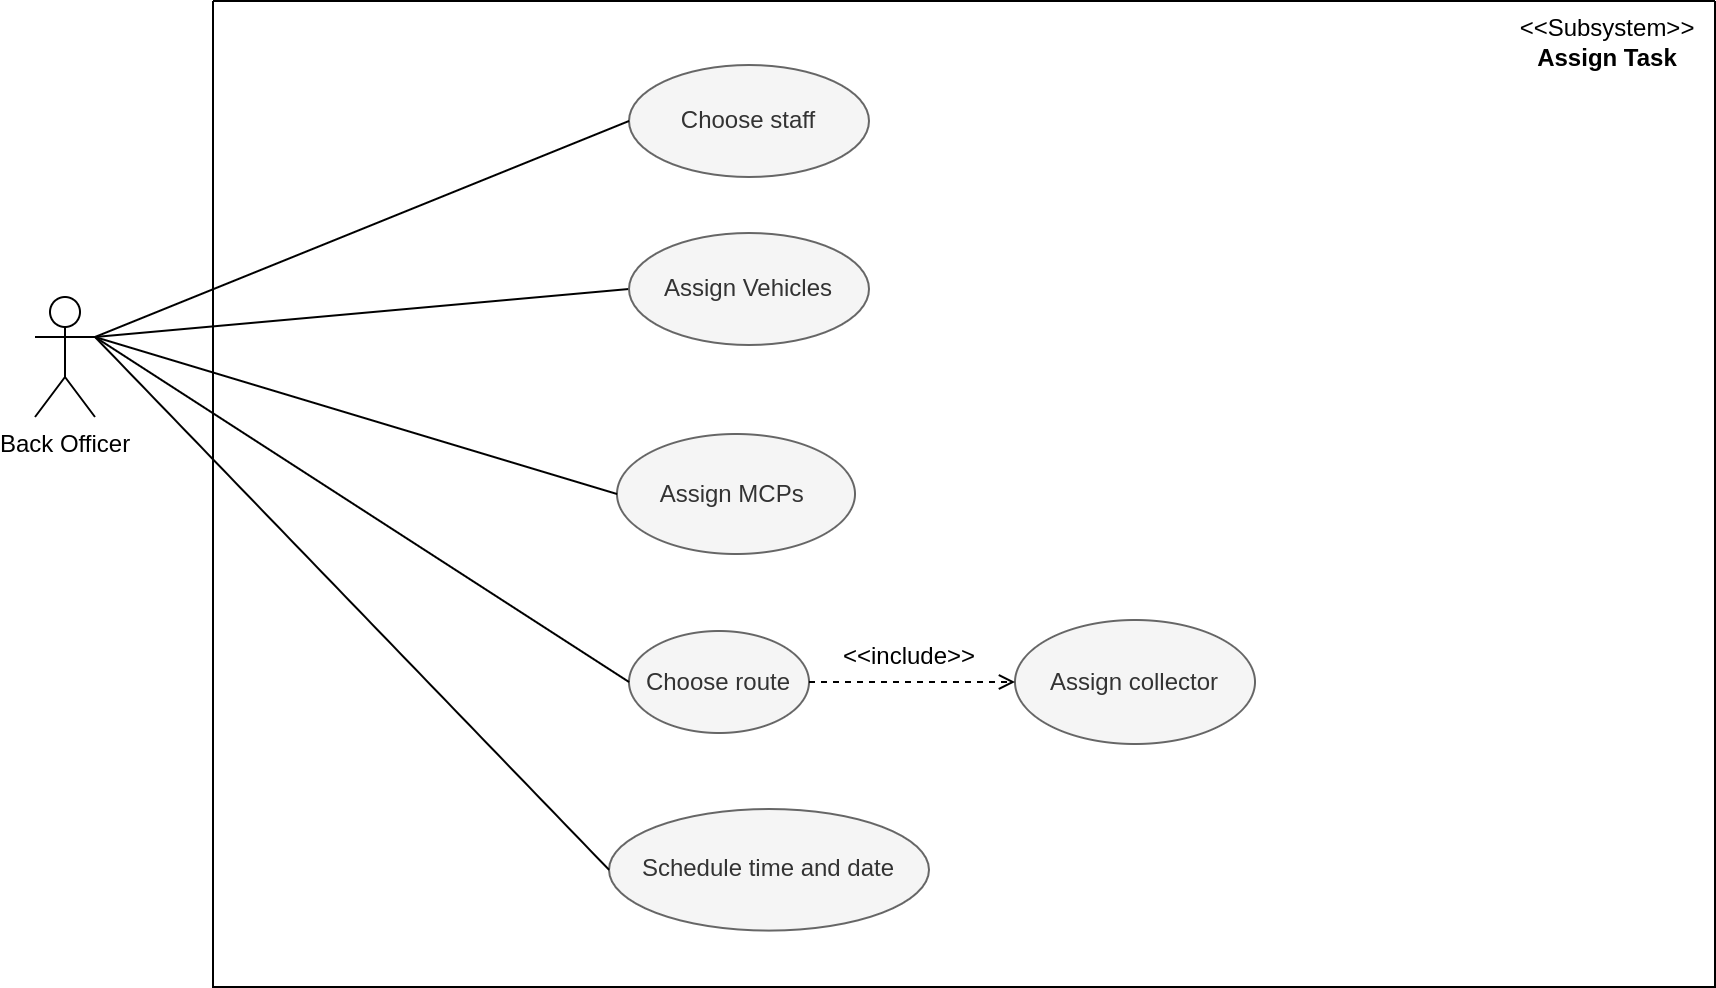
\includegraphics[width=1\linewidth]{imgs/use-case diagram/assignTask_uc.png}
        \caption{Use-case diagram chức năng phân chia công việc}
    \end{figure}

    \vspace{1cm}
    \begin{tblr}{
        width=1\linewidth,
        hlines,
        vlines,
        colspec={X[3]X[7]},
        columns = {valign = m, },
        row{1} = {halign = c, valign = m, bg = lightgray, fg = black},
    }
        {\textbf{Use case name} & \textbf{Choose staff}}  \\
        Description	& Chọn một nhân viên trong hệ thống \\
        Actor & 	Nhân viên giám sát (Back officer) \\
        Trigger & 		Nhân viên giám sát ấn nút chọn công nhân\\
        Pre-condition & Nhân viên giám sát đang ở phần phân công công việc \\
        Post-condition & Công nhân được chọn \\
        Normal flow &   1. Hệ thống lấy dữ liệu về công nhân \newline
                    	2. Hệ thống hiển thị các công nhân \newline
                    	3. Nhân viên giám sát chọn công nhân \newline
                    	4. Hệ thống ghi nhận công nhân được chọn \\
        Alternative flow  & none \\
        Exception flow & none \\
    \end{tblr}

    \begin{tblr}{
        width=1\linewidth,
        hlines,
        vlines,
        colspec={X[3]X[7]},
        columns = {valign = m, },
        row{1} = {halign = c, valign = m, bg = lightgray, fg = black},
    }
        {\textbf{Use case name} & \textbf{Choose vehicle}}  \\
        Description	& Chọn một phương tiện có trong công ty \\
        Actor & 	Nhân viên giám sát (Back officer) \\
        Trigger & 		Nhân viên giám sát ấn nút chọn công nhân\\
        Pre-condition & Nhân viên giám sát đang ở phần phân công công việc \\
        Post-condition & Phương tiện được chọn thành công \\
        Normal flow &   1. Hệ thống lấy dữ liệu về phương tiện \newline
                    	2. Hệ thống hiển thị các phương tiện \newline
                    	3. Nhân viên giám sát chọn phương tiện \newline
                    	4. Hệ thống kiểm tra phương tiện đã được lái hay chưa \newline
                    	5. Hệ thống ghi nhận phương tiện được chọn \\
        Alternative flow  & none \\
        Exception flow & Exception flow thứ 1: tại bước 4 \newline
                    	 1a. Nếu phương tiện đã được gán, thông báo cho người dùng \newline
                    	 Quay lại bước 2 \\
    \end{tblr}

    \vspace{1cm}
    \begin{tblr}{
        width=1\linewidth,
        hlines,
        vlines,
        colspec={X[3]X[7]},
        columns = {valign = m, },
        row{1} = {halign = c, valign = m, bg = lightgray, fg = black},
    }
        {\textbf{Use case name} & \textbf{Assign MCPs}}  \\
        Description	& Gán các điểm MCP cho công nhân \\
        Actor & 	Nhân viên giám sát (Back officer) \\
        Trigger & 	Nhân viên giám sát ấn nút chọn MCPs\\
        Pre-condition & Người quản lý đang ở phần phân công công việc \\
        Post-condition & Các điểm MCP được phân công thành công\\
        Normal flow &   1. Hệ thống lấy dữ liệu về các MCP \newline
                    	2. Hệ thống hiển thị các MCP \newline
                    	3. Nhân viên giám sát chọn MCP \newline
                    	4. Hệ thống ghi nhận các MCP được chọn \\
        Alternative flow  & Alternative flow thứ 1: tại bước 3 \newline
                        	1a. Nếu công nhân được chọn là collector, cho phép gán nhiều MCP \newline
                            \newline
                        	Alternative flow thứ 2: tại bước 3 \newline
                        	2a. Nếu công nhân được chọn là janitor, cho phép gán chỉ 1 MCP \\
        Exception flow & none \\
    \end{tblr}

    \begin{tblr}{
        width=1\linewidth,
        hlines,
        vlines,
        colspec={X[3]X[7]},
        columns = {valign = m, },
        row{1} = {halign = c, valign = m, bg = lightgray, fg = black},
    }
        {\textbf{Use case name} & \textbf{Choose route}}  \\
        Description	& Chọn tuyến đường cho collector \\
        Actor & 	Nhân viên giám sát (Back officer) \\
        Trigger & 	Nhân viên giám sát ấn nút chọn tuyến đường \\
        Pre-condition & Người quản lý đang ở phần phân công công việc \\
        Post-condition & Tuyến đường được chọn\\
        Normal flow &   1. Hệ thống kiểm tra công nhân được chọn là ai \newline
                    	2. Hệ thống hiển thị map trong thành phố \newline
                    	3. Hệ thống hiển thị các tuyến đường được xem là tối ưu \newline
                    	4. Nhân viên giám sát chọn tuyến đường \newline
                    	5. Hệ thống ghi nhận tuyến đường được chọn \\
        Alternative flow  & Alternative flow thứ 1: tại bước 1 \newline
                            1a. Nếu công nhân được chọn là Janitor, hệ thống thông báo và quay 	trở lại màn hình phân công công việc \\
        Exception flow & none \\
    \end{tblr}

    \vspace{1cm}
    \begin{tblr}{
        width=1\linewidth,
        hlines,
        vlines,
        colspec={X[3]X[7]},
        columns = {valign = m, },
        row{1} = {halign = c, valign = m, bg = lightgray, fg = black},
    }
        {\textbf{Use case name} & \textbf{Schedule time and date}}  \\
        Description	& Xếp lịch cho nhân viên \\
        Actor & 	Nhân viên giám sát (Back officer) \\
        Trigger & 	Nhân viên giám sát ấn nút set lịch làm\\
        Pre-condition & Người quản lý đang ở phần phân công công việc \\
        Post-condition & Lịch làm được phân thành công\\
        Normal flow &   1. Hệ thống lấy dữ liệu về lịch làm \newline
                    	2. Hệ thống hiển thị các ngày trong tuần \newline
                    	3. Nhân viên giám sát chọn các ca còn trống \newline
                    	4. Nhân viên xác nhận lịch đã chọn \newline
                    	5. Hệ thống ghi nhận lịch làm \\
        Alternative flow  & none \\
        Exception flow & none \\
    \end{tblr}

\newpage

    

\subsection{Chức năng quản lý tài nguyên (Manage Resources)}
    \begin{figure}[h]
        \centering
        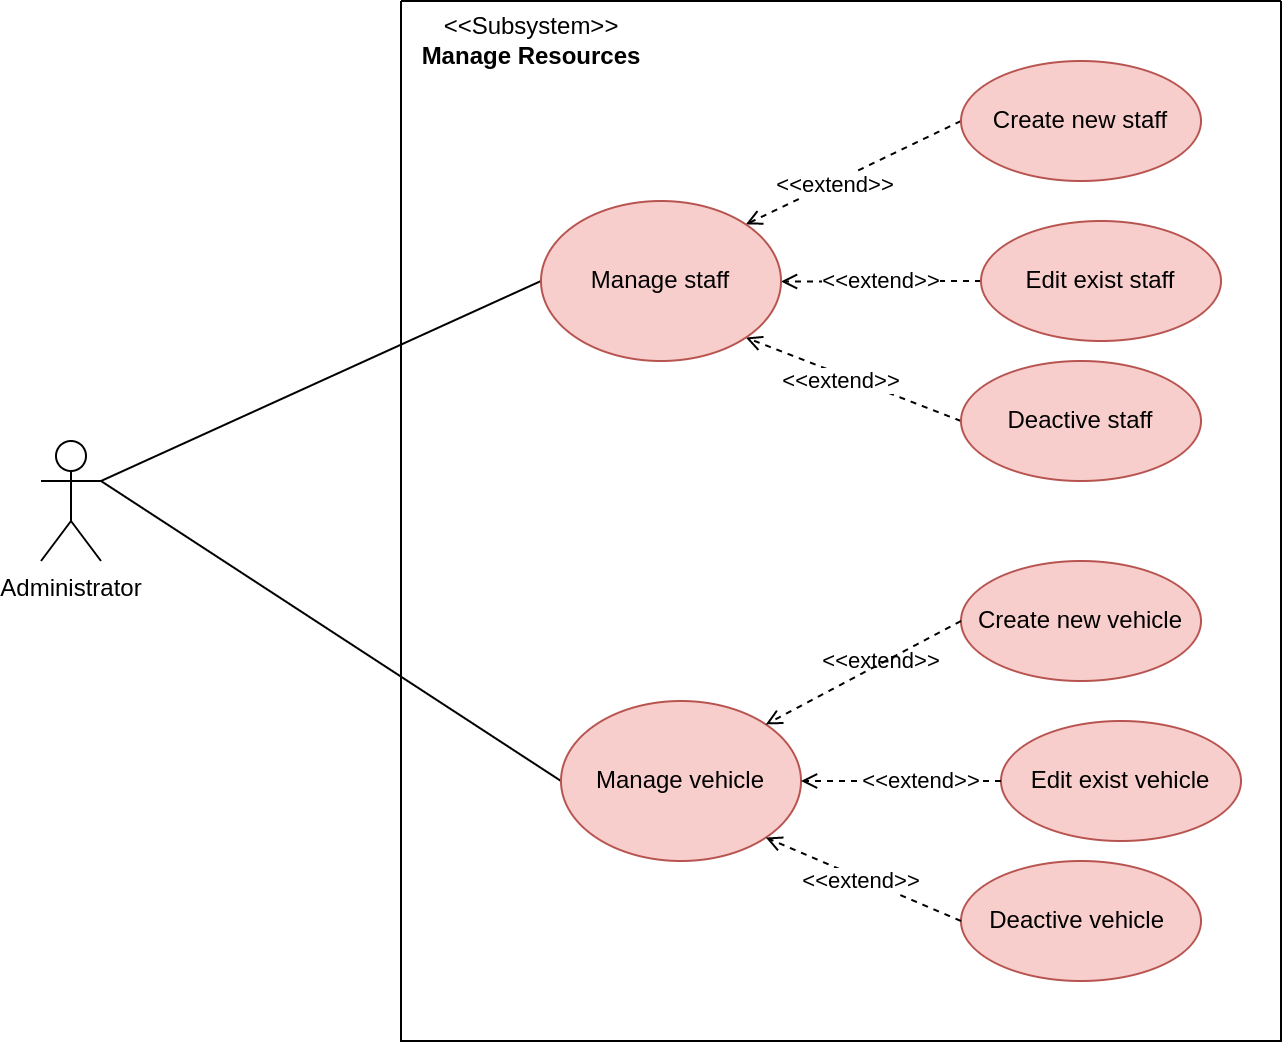
\includegraphics[width=0.70\linewidth]{imgs/use-case diagram/manageResources_uc.png}
        \caption{Use-case diagram chức năng kiểm soát tài nguyên}
    \end{figure}

    \vspace{1cm}
    \begin{tblr}{
        width=1\linewidth,
        hlines,
        vlines,
        colspec={X[3]X[7]},
        columns = {valign = m, },
        row{1} = {halign = c, valign = m, bg = lightgray, fg = black},
    }
        {\textbf{Use case name} & \textbf{Manage staff}}  \\
        Description	& Xếp lịch cho nhân viên \\
        Actor & 	Người quản lý (Administrator) \\
        Trigger & 	Người quản lý ấn vào phần quản lý nhân viên ở menu chính \\
        Pre-condition & Người quản lý đang ở quản lý tài nguyên \\
        Post-condition & Trang quản lý nhân viên được hiển thị \\
        Normal flow &   1. Hệ thống lấy dữ liệu về các nhân viên\newline
                    	2. Hệ thống hiện thị danh sách nhân viên lên màn hình \newline
                    	3. Người dùng chọn một nhân viên để thực hiện hành động \newline
                     	4. Hệ thống hiện thị thông tin chi tiết của nhân viên \\
        Extended points & 	Create new staff \newline
                        	Edit exist staff \newline
                        	Deactive staff \\
    \end{tblr}

    \begin{tblr}{
        width=1\linewidth,
        hlines,
        vlines,
        colspec={X[3]X[7]},
        columns = {valign = m, },
        row{1} = {halign = c, valign = m, bg = lightgray, fg = black},
    }
        {\textbf{Use case name} & \textbf{Create new staff}}  \\
        Description	& Tạo ra một nhân viên mới \\
        Actor & 	Người quản lý (Administrator) \\
        Trigger & 	Người quản lý ấn vào nút tạo người dùng mới \\
        Pre-condition & Người quản lý đang ở trong phần quản lý nhân viên \\
        Post-condition & Nhân viên mới được tạo ra \\
        Normal flow &   1. Hệ thống hiển thị các thông tin cần điền \newline
                    	2. Người dùng điền các thông tin \newline
                    	3. Hệ thống kiểm tra thông tin được điền \newline
                    	4. Người dùng ấn tạo nhân viên mới \newline
                    	5. Hệ thống ghi nhận nhân viên mới \newline
                    	6. Hệ thống thông báo tạo nhân viên thành công \\
        Alternative flow  & Alternative flow thứ 1: tại bước 1 \newline
                        	1a. Người dùng ấn nút hủy \newline
                        	1b. Quay lại màn hình thông tin chi tiết của nhân viên \\
        Exception flow & Exception flow thứ 1: tại bước 3 \newline
                    	 1a. Nếu thông tin sai, thông báo cho người dùng \newline
                    	 Quay lại bước 2  \\
    \end{tblr}

    \vspace{1cm}
    \begin{tblr}{
        width=1\linewidth,
        hlines,
        vlines,
        colspec={X[3]X[7]},
        columns = {valign = m, },
        row{1} = {halign = c, valign = m, bg = lightgray, fg = black},
    }
        {\textbf{Use case name} & \textbf{Edit exist staff}}  \\
        Description	& Chỉnh sửa một nhân viên  \\
        Actor & 	Người quản lý (Administrator) \\
        Trigger & 	Người quản lý ấn vào nút chỉnh sửa nhân viên \\
        Pre-condition & Người quản lý đang ở trong phần quản lý nhân viên \\
        Post-condition & Thông tin nhân viên được chỉnh sửa thành công\\
        Normal flow &   1. Hệ thống hiển thị các thông tin cần điền \newline
                    	2. Người dùng điền các thông tin \newline
                    	3. Hệ thống kiểm tra thông tin được điền \newline
                    	4. Người dùng ấn cập nhật nhân viên \newline
                    	5. Hệ thống ghi nhận thông tin được cập nhật \newline
                    	6. Hệ thống thông báo cập nhật nhân viên thành công \\
        Alternative flow  & Alternative flow thứ 1: tại bước 1 \newline
                        	1a. Người dùng ấn nút hủy \newline
                        	1b. Quay lại màn hình thông tin chi tiết của nhân viên \\
        Exception flow & Exception flow thứ 1: tại bước 3 \newline
                    	 1a. Nếu thông tin sai, thông báo cho người dùng \newline
                    	 Quay lại bước 2 \\
    \end{tblr}

    \begin{tblr}{
        width=1\linewidth,
        hlines,
        vlines,
        colspec={X[3]X[7]},
        columns = {valign = m, },
        row{1} = {halign = c, valign = m, bg = lightgray, fg = black},
    }
        {\textbf{Use case name} & \textbf{Deactive staff}}  \\
        Description	& Hủy kích hoạt một nhân viên \\
        Actor & 	Người quản lý (Administrator) \\
        Trigger & 	Người quản lý ấn vào nút hủy kích hoạt nhân viên \\
        Pre-condition & Người quản lý đang ở trong phần quản lý nhân viên \\
        Post-condition & Nhân viên bị hủy kích hoạt\\
        Normal flow &   1. Hệ thống hiểu thị xác nhận hủy kích hoạt nhân viên \newline
                    	2. Người dùng nhấn đồng ý \newline
                    	3. Hệ thống hủy kích hoạt nhân viên \newline
                    	4. Hệ thống thông báo hủy kích hoạt thành công \\
        Alternative flow  & Alternative flow thứ 1: tại bước 1 \newline
                        	1a. Người dùng ấn nút hủy \newline
                        	1b. Quay lại màn hình thông tin chi tiết của nhân viên \\
        Exception flow & none \\
    \end{tblr}

    \vspace{1cm}
    \quad Phần use-case senario của  Manage vehicle tương tự như trên.


	
\section{Activity diagram giữa hệ thống và các bên liên quan trong Task Assignment Module}
    \begin{figure}[h]
        \centering
        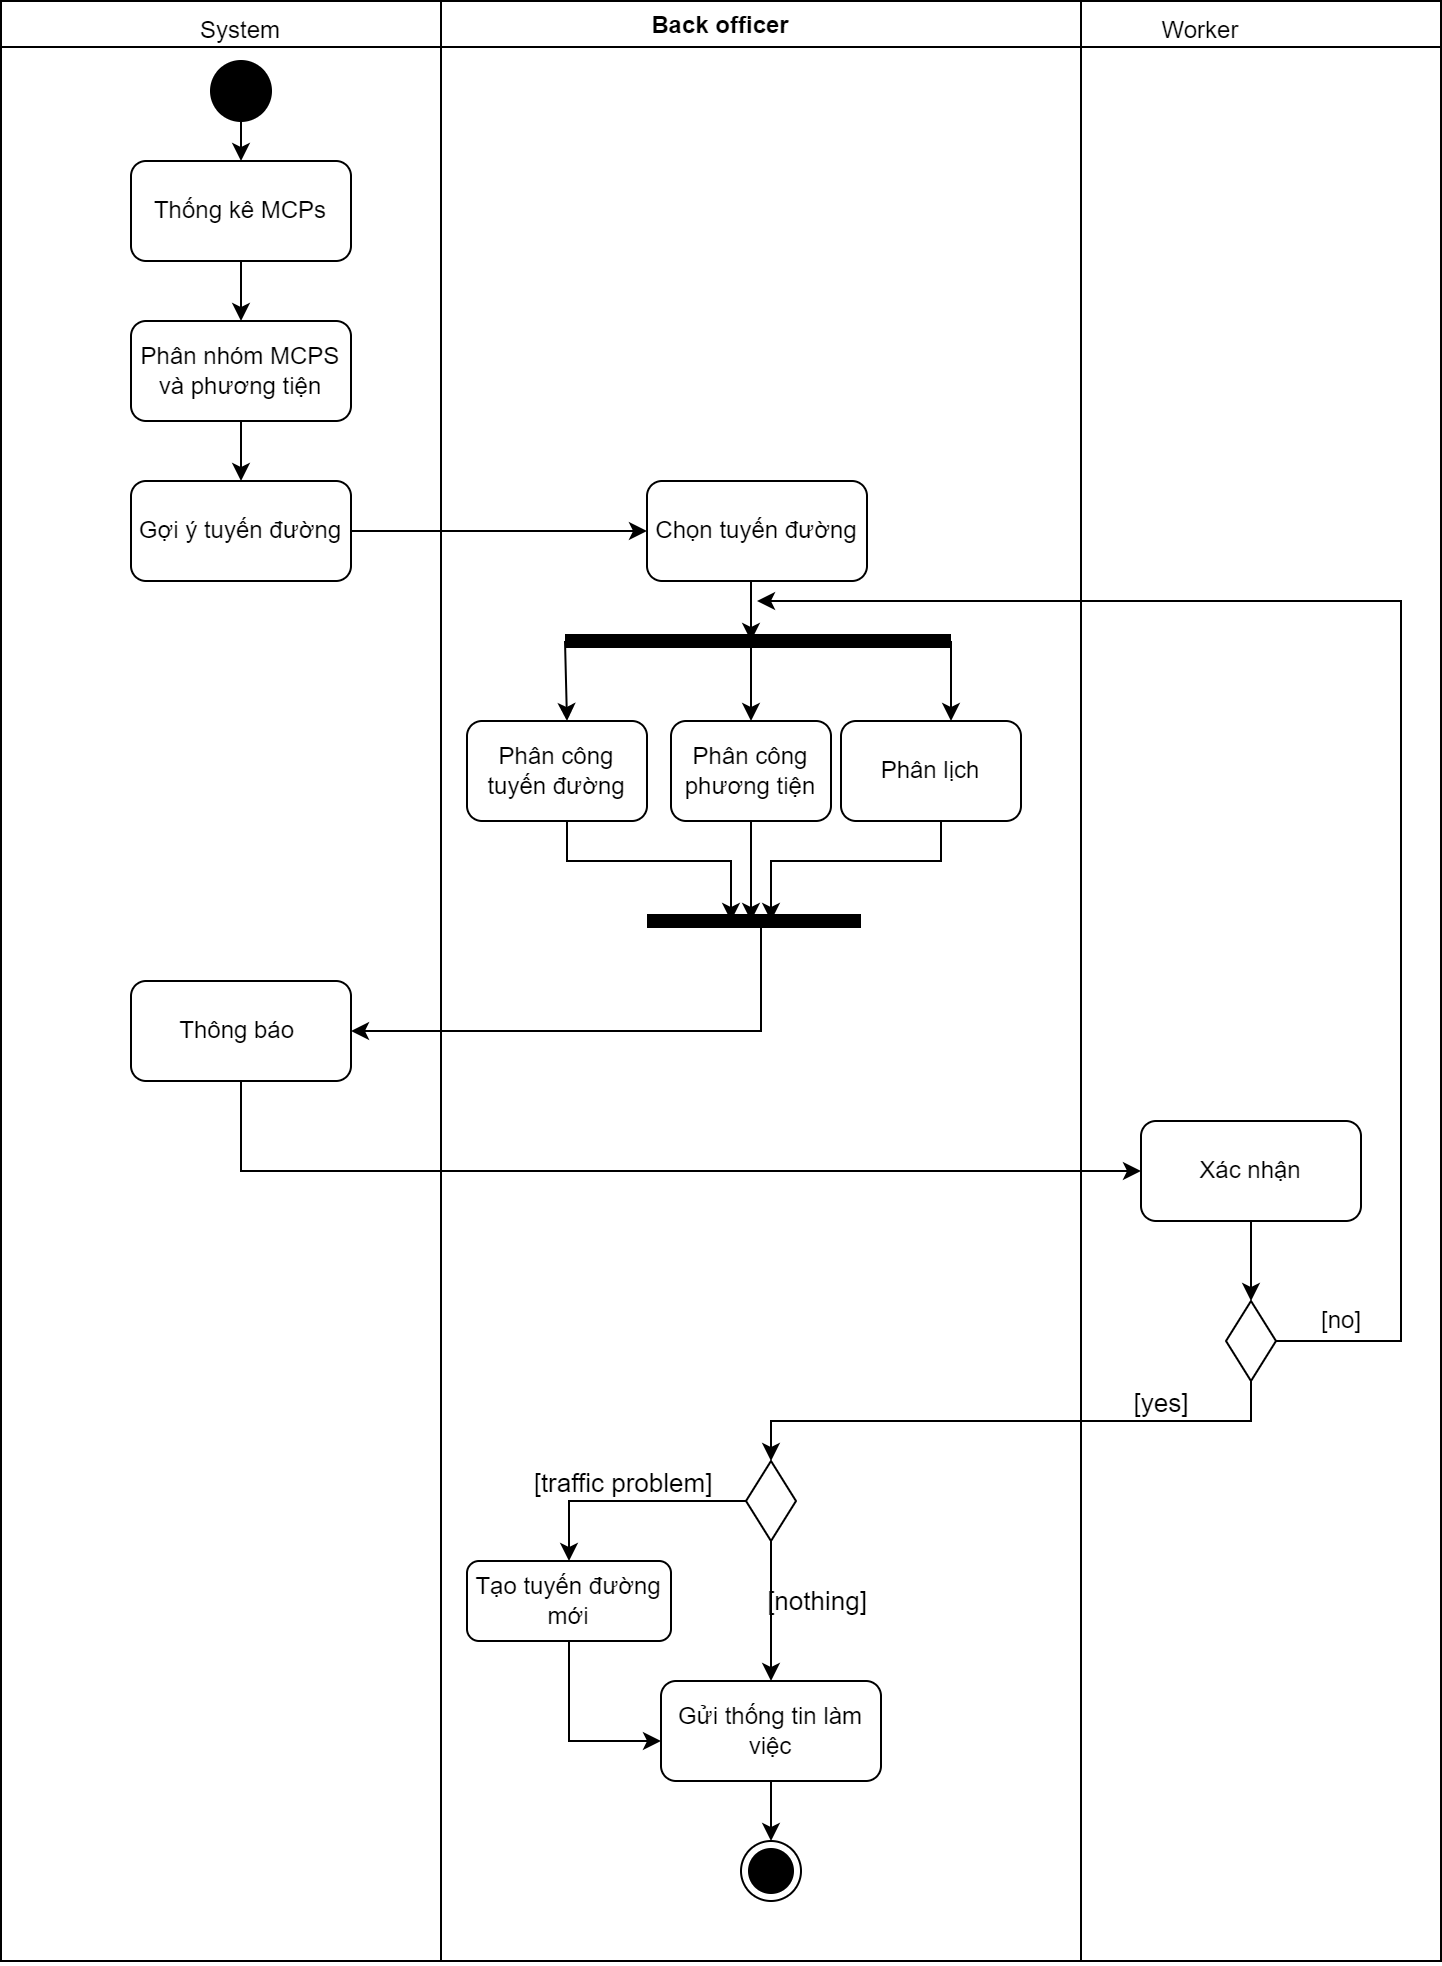
\includegraphics[width=15.0cm,height=15cm]{imgs/activity diagram/activity diagram.png}
        \caption{Activity diagram trong Task Asssignment Module}
    \end{figure}
    \newpage
    Hoạt động giữa hệ thống và các bên liên quan trong Task Assignment Module gồm các hoạt động theo thứ tự:
    \begin{enumerate}
        \item Bắt đầu.
        \item Hệ thống thống kê số lượng, vị trí MCPs.
        \item Hệ thống phân nhóm MCPs theo vùng phù hợp với sức chứa của phương tiện hiện có để tối ưu về tuyến đường và nhiên liệu.
        \item Hệ thống gợi ý các tuyến đường tối ưu cho Back officer.
        \item Back officer chọn tuyến đường cho tháng.
        \item Back officer phân công tuyến đường, phân phương tiện và tạo lịch cho collectors, janitors.
        \item Hệ thống gửi thông báo cho collectors, janitors.
        \item  Collectors, janitors xem thông báo được gửi.
        \item Back officer gửi thông tin làm việc theo ngày cho collectors, janitors.
        \item Kết thúc
    \end{enumerate}

\section{Giải pháp ý niệm cho task Route planning và Sequence diagram mô tả nó}
    \subsection{Giải pháp ý niệm cho task Route Planning}
        \textbf{Xét các Actor: }
    
        \begin{itemize}
            \item[-] Back Officer.
            \item[-] Cơ sở dữ liệu bản đồ (Map Database): một API cung cấp mọi thông tin về đường đi trong một vùng không gian nhất định khi được yêu cầu.
        \end{itemize}
    
        \textbf{Giả định:}
    
        \begin{itemize}
            \item[-] Back Officer đã đăng nhập thành công vào hệ thống.
            \item[-] Back Officer đã thao tác với hệ thống, đã nạp một danh sách các MCPs mà mình có nhu cầu tìm đường.
            \item[-] Map Database luôn hoạt động và hoạt động đúng kỳ vọng.
        \end{itemize}
    
        \textbf{Ta có, các entity liên quan:}
    
        \begin{itemize}
            \item[-] UIController: Hệ thống đảm nhiệm chức năng làm cầu nối, cho phép người dùng quản lý, sử dụng hệ thống.
            \item[-] RoutePlannerObject: Hệ thống đảm nhiệm chính chức năng tìm đường tự động và đánh giá đường đi.
        \end{itemize}
    
        \textbf{Các thao tác có thể thực hiện}
    
        \begin{itemize}
            \item[-] Back officer ra lệnh cho hệ thống tự tạo đường đi (route) phù hợp.
            \item[-] Back officer tự chỉnh sửa, thêm bớt các tuyến đường trong route mới hoặc route đã định sẵn từ thao tác trên.
        \end{itemize}
    
        \textbf{Mô tả chi tiết các thao tác}
        \begin{enumerate}
            \item Back officer ra lệnh cho hệ thống tự tạo đường đi (route) phù hợp.
            \begin{itemize}
                \item[-] Người dùng thực hiện lệnh tạo route tự động bằng cách ra lệnh GenerateRoute () lên hệ thống.
                \item[-] UIController nhận lệnh, thực hiện lệnh PlanRoute (MCPs, vehicles) lên hệ thống RoutePlannerObject với MCPs, vehicles là các MCP và phương tiện được dùng.
                \item[-] RoutePlannerObject thực hiện GetAvailablePaths (locations, vehicles) đối với Map Database để lấy đường đi hợp lệ giữa các vị trí của MCP mà phương tiện có thể di chuyển qua.
                \begin{itemize}
                    \item[+] Nếu tồn tại những đường đi hợp lệ, RoutePlannerObject tính toán route tốt nhất và trả về cho UIController. UIController trình thông tin về người dùng. Quá trình tự động tạo route kết thúc thành công.
                    \item[+] Nếu không tồn tại path nào, RoutePlannerObject trả về lỗi không tồn tại đường đi cho UIController. Quá trình tự động tạo route kết thúc không thành công.
                \end{itemize}
            \end{itemize}
        
            \item Back officer tự chỉnh sửa, thêm bớt các tuyến đường trong route mới hoặc route đã định sẵn từ thao tác trên.
            \begin{itemize}
                \item[-] UIController tự chờ mỗi khi người dùng chỉnh sửa, thêm/ bớt route trên giao diện, chạy lệnh ModifyRoute (route) với route là tổng hợp các route mới (mà người dùng đã thay đổi/ chỉnh sửa).
                \item[-] UIController tìm các path có trong route mới, qua lệnh ValidateRoute (paths, MCPs, vehicles) gửi paths vừa chỉnh sửa cho hệ thống RoutePlannerObject để đánh giá tính hợp lệ và hiệu quả.
                \item[-] RoutePlannerObject lấy những đường đi hợp lệ cho phương tiện giữa các MCP từ hệ cơ sở dữ liệu bản đồ bằng lệnh GetPathsBetween (locations, vehicles).
                \item[-] RoutePlannerObject đánh giá nếu đường đi trong route có hợp lệ so với các paths trên bản đồ.
                \begin{itemize}
                    \item[+] Nếu route là hợp lệ, trả về UIController độ hiệu quả của route. UIController trình thông tin đến người dùng và lưu route vào hệ thống. Quá trình chỉnh sửa/ thay đổi route thành công.
                    \item[+] Nếu route là không hợp lệ, trả về UIController sự hợp lệ của route. UIController trình thông tin đến người dùng, không lưu route mới vào hệ thống. Quá trình chỉnh sửa/ thay đổi route không thành công.
                \end{itemize}
            \end{itemize}
        \end{enumerate}
    \subsection{Sequence diagram mô tả giải pháp cho task Route Planning}
        \begin{figure}[H]
            \centering
            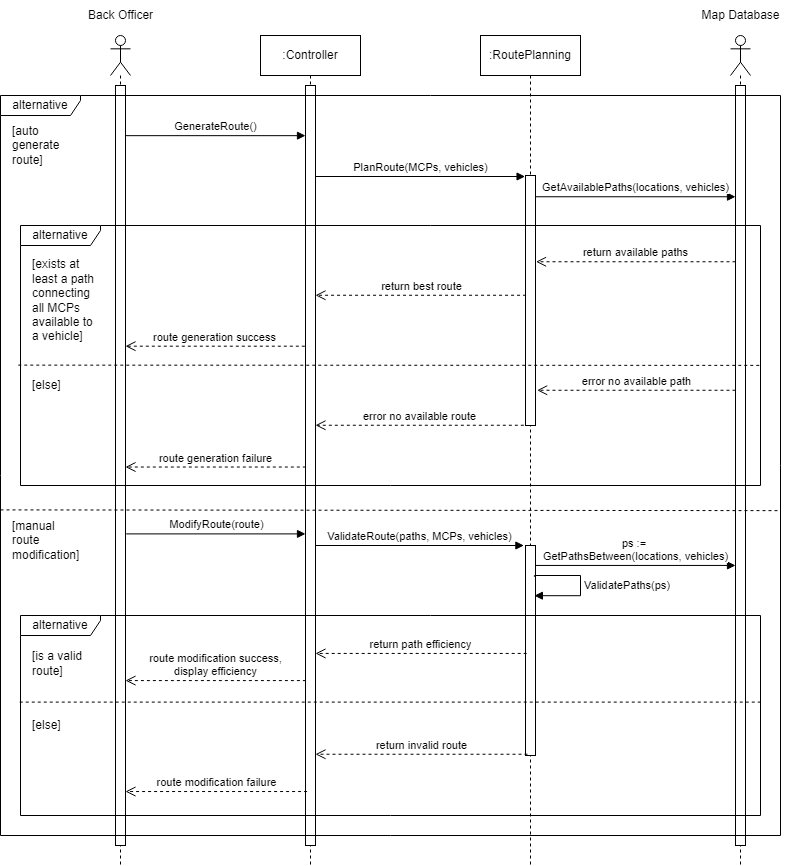
\includegraphics[width=1\linewidth]{imgs/sequence diagram/Sequence Diagram 2.2.png}
            \caption{Sequence diagram cho Task Route Planning}
        \end{figure}
    
        \newpage

\section{Class Diagram cho task assignment module}
     \begin{figure}[h]
        \centering
        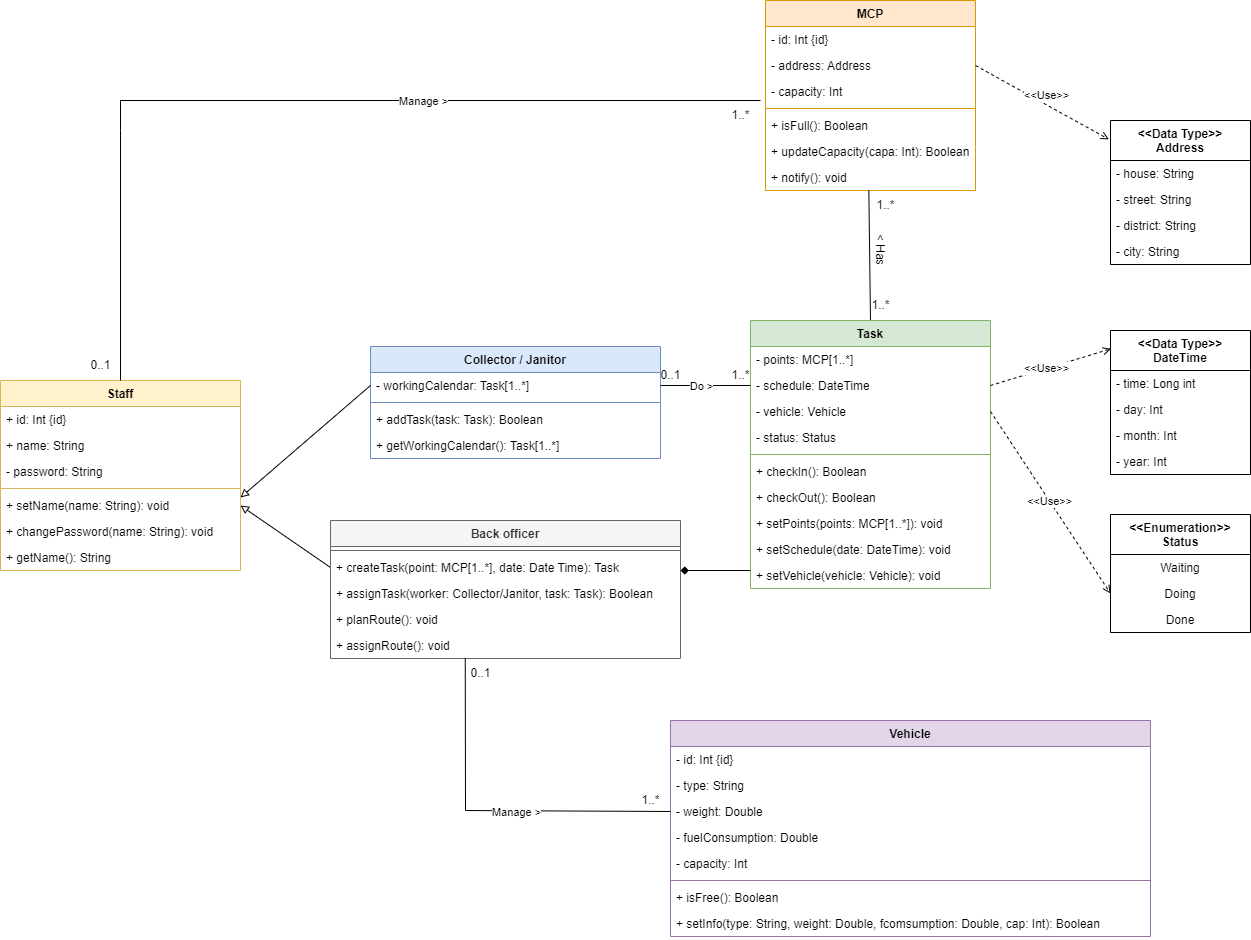
\includegraphics[width=15cm,height=15cm]{imgs/class diagram/class diagram.png}
        \caption{Class diagram cho task assignment module}
    \end{figure}

    \newpage
    -Có tất cả 6 class trong module trên gồm có:
    \begin{enumerate}
        \item Class Staff:
        \begin{table}[htp]
            \begin{tabular}{|lll|}
                \hline
                \multicolumn{1}{|l|}{Class Name} & \multicolumn{2}{l|}{Staff}                                     \\ \hline
                \multicolumn{1}{|l|}{Inherit}    & \multicolumn{2}{l|}{None}                                      \\ \hline
                \multicolumn{3}{|c|}{\cellcolor[HTML]{FFFFC7}Attributes}                                          \\ \hline
                \multicolumn{1}{|l|}{int}        & \multicolumn{1}{l|}{id}               & Số định danh nhân viên \\ \hline
                \multicolumn{1}{|l|}{string}     & \multicolumn{1}{l|}{name}             & Tên nhân viên          \\ \hline
                \multicolumn{1}{|l|}{string}     & \multicolumn{1}{l|}{password}         & Mật khẩu đăng nhập     \\ \hline
                \multicolumn{3}{|c|}{\cellcolor[HTML]{FFFFC7}Methods}                                             \\ \hline
                \multicolumn{1}{|l|}{void}       & \multicolumn{1}{l|}{setName()}        & Đặt tên cho nhân viên  \\ \hline
                \multicolumn{1}{|l|}{void}       & \multicolumn{1}{l|}{changePassword()} & Đổi mật khẩu           \\ \hline
                \multicolumn{1}{|l|}{string}     & \multicolumn{1}{l|}{getName()}        & Lấy tên nhân viên      \\ \hline
                \multicolumn{3}{|c|}{\cellcolor[HTML]{FFFFC7}Relationships}                                       \\ \hline
                \multicolumn{1}{|l|}{Manage}     & \multicolumn{2}{l|}{Quản lý thông tin các MCP}                 \\ \hline
            \end{tabular}
        \end{table}
                
        \item Class Collector / Janitor:
        \begin{table}[htp]
            \begin{tabular}{|lll|}
                \hline
                \multicolumn{1}{|l|}{Class Name} & \multicolumn{2}{l|}{Collector/Janitor}                              \\ \hline
                \multicolumn{1}{|l|}{Inherit}    & \multicolumn{2}{l|}{Staff}                                          \\ \hline
                \multicolumn{3}{|c|}{\cellcolor[HTML]{FFFFC7}Attributes}                                               \\ \hline
                \multicolumn{1}{|l|}{Task{[}{]}} & \multicolumn{1}{l|}{workingCalendar}      & Lịch làm việc           \\ \hline
                \multicolumn{3}{|c|}{\cellcolor[HTML]{FFFFC7}Methods}                                                  \\ \hline
                \multicolumn{1}{|l|}{boolean}    & \multicolumn{1}{l|}{addTask()}            & Thêm task vào phần lịch \\ \hline
                \multicolumn{1}{|l|}{Task{[}{]}} & \multicolumn{1}{l|}{getWorkingCalendar()} & Lấy, xem lịch làm việc  \\ \hline
                \multicolumn{3}{|c|}{\cellcolor[HTML]{FFFFC7}Relationships}                                            \\ \hline
                \multicolumn{1}{|l|}{Do}         & \multicolumn{2}{l|}{Collector và Janitor thực hiện task}            \\ \hline
            \end{tabular}
        \end{table}
            
        \item Class Back officer:
        \begin{table}[htp]
            \begin{tabular}{|lll|}
                \hline
                \multicolumn{1}{|l|}{Class Name}  & \multicolumn{2}{l|}{Back officer}                                     \\ \hline
                \multicolumn{1}{|l|}{Inherit}     & \multicolumn{2}{l|}{Staff}                                            \\ \hline
                \multicolumn{3}{|c|}{\cellcolor[HTML]{FFFFC7}Attributes}                                                  \\ \hline
                \multicolumn{3}{|c|}{\cellcolor[HTML]{FFFFC7}Methods}                                                     \\ \hline
                \multicolumn{1}{|l|}{Task}        & \multicolumn{1}{l|}{createTask()} & Tạo task                          \\ \hline
                \multicolumn{1}{|l|}{boolean}     & \multicolumn{1}{l|}{assignTask()} & Gán task cho collector và janitor \\ \hline
                \multicolumn{1}{|l|}{void}        & \multicolumn{1}{l|}{planRoute()}  & Tạo tuyến đường                   \\ \hline
                \multicolumn{3}{|c|}{\cellcolor[HTML]{FFFFC7}Relationships}                                               \\ \hline
                \multicolumn{1}{|l|}{Manage}      & \multicolumn{2}{l|}{Quản lý thông tin phương tiện}                    \\ \hline
                \multicolumn{1}{|l|}{Composition} & \multicolumn{2}{l|}{Bao gồm task}                                     \\ \hline
            \end{tabular}
        \end{table}
    
        \newpage
            
        \item Class Task:
        \begin{table}[htp]
            \begin{tabular}{|lll|}
                \hline
                \multicolumn{1}{|l|}{Class Name} & \multicolumn{2}{l|}{Task}                                          \\ \hline
                \multicolumn{1}{|l|}{Inherit}    & \multicolumn{2}{l|}{None}                                          \\ \hline
                \multicolumn{3}{|c|}{\cellcolor[HTML]{FFFFC7}Attributes}                                              \\ \hline
                \multicolumn{1}{|l|}{MCP{[}{]}}  & \multicolumn{1}{l|}{points}        & Danh sách các MCP của task    \\ \hline
                \multicolumn{1}{|l|}{DateTime}   & \multicolumn{1}{l|}{schedule}      & Thời gian làm cho task        \\ \hline
                \multicolumn{1}{|l|}{Vehicle}    & \multicolumn{1}{l|}{vehicle}       & Phương tiện dùng cho task     \\ \hline
                \multicolumn{1}{|l|}{Status}     & \multicolumn{1}{l|}{status}        & Trạng thái của task           \\ \hline
                \multicolumn{3}{|c|}{\cellcolor[HTML]{FFFFC7}Methods}                                                 \\ \hline
                \multicolumn{1}{|l|}{boolean}    & \multicolumn{1}{l|}{checkIn()}     & check in task                 \\ \hline
                \multicolumn{1}{|l|}{boolean}    & \multicolumn{1}{l|}{checkOut()}    & check out task                \\ \hline
                \multicolumn{1}{|l|}{void}       & \multicolumn{1}{l|}{setPoints()}   & Đặt danh sách MCP cho task    \\ \hline
                \multicolumn{1}{|l|}{void}       & \multicolumn{1}{l|}{setSchedule()} & Đặt lịch cho task             \\ \hline
                \multicolumn{1}{|l|}{void}       & \multicolumn{1}{l|}{setVehicle()}  & Đặt phương tiện dùng cho task \\ \hline
                \multicolumn{3}{|c|}{\cellcolor[HTML]{FFFFC7}Relationships}                                           \\ \hline
                \multicolumn{1}{|l|}{Has}        & \multicolumn{2}{l|}{Mang thông tin các MCP}                        \\ \hline
            \end{tabular}
        \end{table}
            
            
        \item Class Vehicle:
        \begin{table}[htp]
            \begin{tabular}{|lll|}
                \hline
                \multicolumn{1}{|l|}{Class Name} & \multicolumn{2}{l|}{Vehicle}                                                               \\ \hline
                \multicolumn{1}{|l|}{Inherit}    & \multicolumn{2}{l|}{None}                                                                  \\ \hline
                \multicolumn{3}{|c|}{\cellcolor[HTML]{FFFFC7}Attributes}                                                                      \\ \hline
                \multicolumn{1}{|l|}{int}        & \multicolumn{1}{l|}{id}              & Số định danh phương tiện                            \\ \hline
                \multicolumn{1}{|l|}{string}     & \multicolumn{1}{l|}{type}            & Loại phương tiện                                    \\ \hline
                \multicolumn{1}{|l|}{double}     & \multicolumn{1}{l|}{weight}          & Khối lượng phương tiện                              \\ \hline
                \multicolumn{1}{|l|}{double}     & \multicolumn{1}{l|}{fuelConsumption} & Mức tiêu thụ nhiên liệu                             \\ \hline
                \multicolumn{1}{|l|}{int}        & \multicolumn{1}{l|}{capacity}        & Sức chứa của phương tiện                            \\ \hline
                \multicolumn{3}{|c|}{\cellcolor[HTML]{FFFFC7}Methods}                                                                         \\ \hline
                \multicolumn{1}{|l|}{boolean}    & \multicolumn{1}{l|}{isFree()}        & Kiểm tra phương tiện có đang được sử dụng hay không \\ \hline
                \multicolumn{1}{|l|}{boolean}    & \multicolumn{1}{l|}{setInfo()}       & Đặt thông tin cho phương tiện                       \\ \hline
                \multicolumn{3}{|c|}{\cellcolor[HTML]{FFFFC7}Relationships}                                                                   \\ \hline
            \end{tabular}
        \end{table}
            
        \newpage
        \item Class MCP:
        \begin{table}[htp]
            \begin{tabular}{|lll|}
                \hline
                \multicolumn{1}{|l|}{Class Name} & \multicolumn{2}{l|}{MCP}                                                            \\ \hline
                \multicolumn{1}{|l|}{Inherit}    & \multicolumn{2}{l|}{None}                                                           \\ \hline
                \multicolumn{3}{|c|}{\cellcolor[HTML]{FFFFC7}Attributes}                                                               \\ \hline
                \multicolumn{1}{|l|}{int}        & \multicolumn{1}{l|}{id}               & Số định danh cho MCP                        \\ \hline
                \multicolumn{1}{|l|}{Address}    & \multicolumn{1}{l|}{address}          & Địa chỉ của MCP                             \\ \hline
                \multicolumn{1}{|l|}{int}        & \multicolumn{1}{l|}{capacity}         & Sức chứa của MCP                            \\ \hline
                \multicolumn{1}{|l|}{int}        & \multicolumn{1}{l|}{capacity}         & Sức chứa của phương tiện                    \\ \hline
                \multicolumn{3}{|c|}{\cellcolor[HTML]{FFFFC7}Methods}                                                                  \\ \hline
                \multicolumn{1}{|l|}{boolean}    & \multicolumn{1}{l|}{isFull()}         & Kiểm tra MCP có đang đầy chỗ chứa hay không \\ \hline
                \multicolumn{1}{|l|}{boolean}    & \multicolumn{1}{l|}{updateCapacity()} & Cập nhật lại sức chứa MCP                   \\ \hline
                \multicolumn{1}{|l|}{void}       & \multicolumn{1}{l|}{notify()}         & Thông báo khi MCP hết sức chứa              \\ \hline
                \multicolumn{3}{|c|}{\cellcolor[HTML]{FFFFC7}Relationships}                                                            \\ \hline
            \end{tabular}
        \end{table}
\end{enumerate}

	\section{Mô tả thiết kế kiến trúc để xây dựng hệ thống}
    \quad Sau khi xác định rõ bài toàn, dựa trên những yêu cầu cả về mặt chứng năng và phi chức năng, nhóm quyết định đưa ra thiết kế hệ thống như sau:

    \vspace{1cm}
    \begin{figure}[h]
    	\centering
    	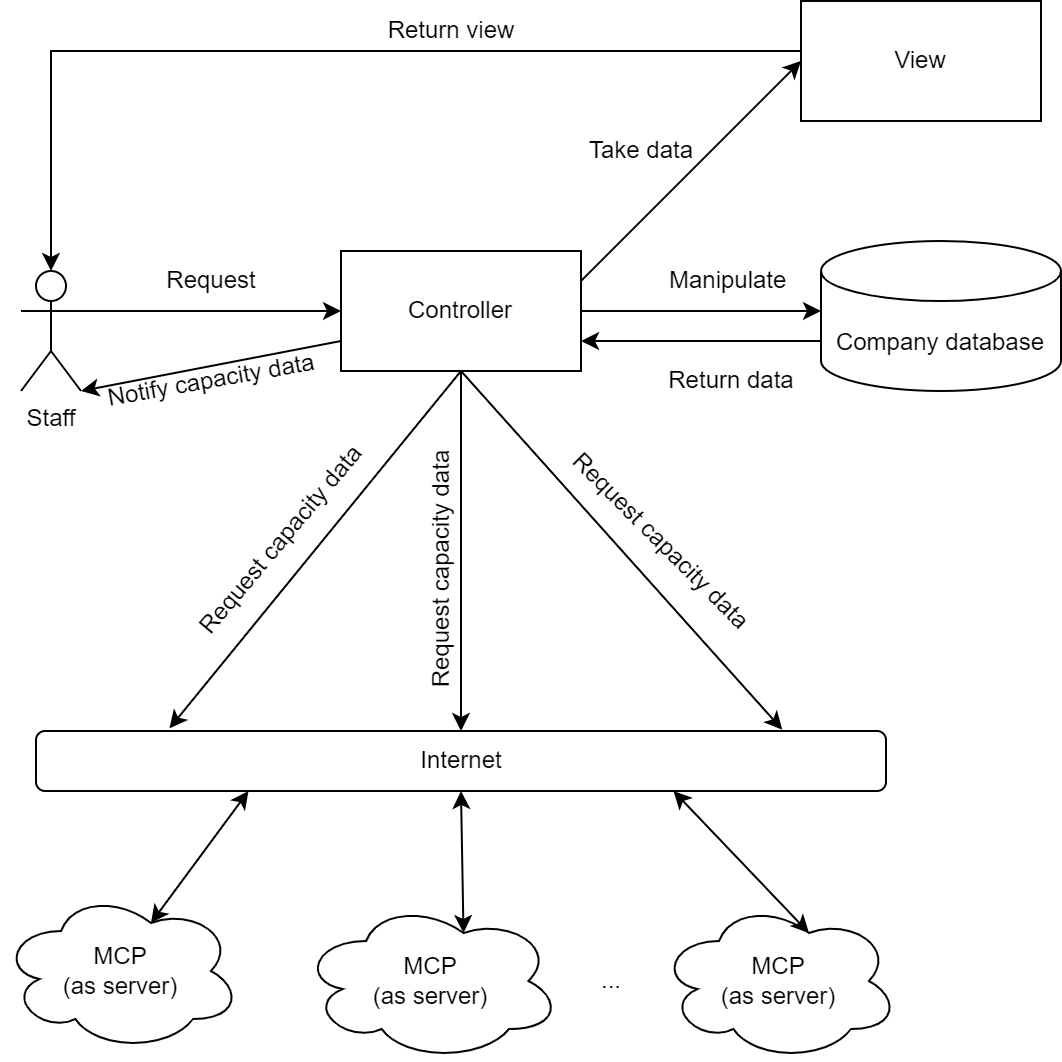
\includegraphics[width=1\linewidth]{imgs/architecture design.png}
    	\caption{Thiết kế kiến trúc của hệ thống}
    \end{figure}

   	\begin{tblr}{
   			width=1\linewidth,
   			hlines,
   			vlines,
   			colspec={X[3]X[7]},
   			columns = {valign = m, },
			column{1} = {halign = c},
   			row{1} = {halign = c, valign = m, bg = lightgray, fg = black},
   		}
   		{\textbf{Table} & \textbf{Architecture design}}  \\
   		Pattern		& 	MVC + Pub-sub \\
   		Description & 	1. Với các thông tin cơ bản như thông tin cá nhân, lịch làm, thông tin về phương tiện, ta sử dụng mô hình MVC để lấy dữ liệu và hiển thị lên cho người dùng. \newline
						\newline
		   				2. Với các thông tin về sức chứa của các MCP, ta sử dụng mô hình publisher - subscriber với Controller đóng vai trò là subscriber và MCP là các publisher. \newline
						\newline
		   				3. Với các thông báo về việc sức chứa của các MCP đạt mức tối đa ta sử dụng mô hình publisher - subscriber với Controller lúc này đóng vai trò là publisher và nhân viên là các subscriber. \\
		Flow & 			1. Controller nhận request từ người dùng -> gọi đến database thực hiện yêu cầu -> database gửi kết qua sau khi thực hiện lại cho controller -> controller gửi dữ liệu vừa nhận được cho phần View -> View hiển thị kết quả cho người dùng. \newline
						\newline
						2. Controller nhận dữ liệu từ tất cả các sensor của từng MCP sau mỗi 15 phút. Nếu sau ba lần controller không nhận được dữ liệu, sensor xem như bị mất kết nối và thực hiện thiết lập lại kết nối với sensor của MCP đó. \newline
						\newline
						3. Ngay sau khi nhận dữ liệu từ các sensor, controller thực hiện broadcast dữ liệu nếu sức chứa đã đầy đến collector/janitor liên quan đến MCP đó. \\
   	\end{tblr}

   	\vspace{0.5cm}

	\quad \textbf{Những nguyên nhân nhóm chọn kiến trúc trên:}
	\begin{enumerate}
		\item[-] MCP (Model - Controller - View) là kiểu kiến trúc bao gồm 3 chủ thể lớn là Controller - đảm nhiệm việc kiểm tra và thực hiện các yêu cầu được gửi đến, Model - đảm nhiệm việc truy suất dữ liệu của hệ thống và View - là cái được trả về cho người dùng, cái được hiển thị trên màn hình. MCP phù hợp với yêu cầu hiện thực ứng dụng trên nền tảng web, dễ dàng trong việc thiết kế, triển khai hệ thống.
		\item[-] Publisher - Subcriber cho cho phép hệ thống nhận thông tin liên tục về các điểm MCP và gửi đến người dùng những thông tin kịp thời nhất khi một hay nhiều điểm MCP bị đầy.
		\item[-] Xét tương đối với các kiến trúc khác:
		\begin{enumerate}
			\item[+] Mặc dù Layer và MCV đều được thiết kế theo kiểu module, trong đó các khối được tách ra đảm nhiệm từng chức năng riêng biệt, khi cần nâng cấp một module sẽ không ảnh hưởng đến hoạt động của các module khác. Tuy nhiên MVC có hiệu suất tốt hơn Layer, vì dữ liệu được truyền qua một tầng duy nhất, khác với việc khi truyền dữ liệu ở kiến trúc Layer phải đi qua nhiều lớp dẫn tới hao phí thời gian truyển dữ liệu từ lớp này sang lớp kia
			\item[+] Peer-to-Peer là kiểu thiết kế trong đó các client sẽ kết nối trực tiếp với nhau, trong trường hợp ứng dụng quản lý có số lượng lớn các client (bao gồm back officer, janitor, collect), việc kết nối trực tiếp các thiết bị sẽ gây ra sự chồng chéo, khó khăn trong việc kiểm soát cũng như bảo trì
			\item[+] Pipe-filter có lợi thế trong việc tách dữ liệu có độ phức tạp cao thành dữ liệu sạch thông qua các lớp màn lọc (filter), tuy nhiên hạn chế của kién trúc này là ở việc với những nguồn data khác nhau, nó sẽ yêu cầu một luồng riêng, khả năng tái sử dụng các luồng cũ rất thấp. Đối với bài toán mà nhóm đang giải quyết, việc dữ liệu mà các MCP trả về là khác nhau, nguyên nhân có thể do sự khác biệt về phần cứng hay phần mềm của các cảm biến, chính vì thế nếu sử dụng Pipe-filter thì ta phải tạo ra nhiều luồng xử lý đối với từng MCP.
		\end{enumerate}
	\end{enumerate}
  
	\newpage
   	\quad Đối với bài toán được đặt ra, ta sẽ có tổng cộng 6 module. Bao gồm:
   	\begin{enumerate}
   		\item Module Xác thực

   		\begin{tblr}{
   				width=1\linewidth,
   				hlines,
   				vlines,
   				colspec={X[3]X[7]},
   				columns = {valign = m, },
   			}
   			Input & Người dùng X \\
   			Output & Người dùng X có được truy cập hay không \newline
   					 Vai trò của người dùng X là gì \\
   			Method & Validation() \newline
   			 		 Login() \newline
   			 		 Logout() \newline
   			 		 ChangePassword() \\
   		\end{tblr}

   		\item Module Chat

  		\begin{tblr}{
  				width=1\linewidth,
  				hlines,
  				vlines,
  				colspec={X[3]X[7]},
  				columns = {valign = m, },
  			}
  			Input & Tin nhắn, văn bản\\
  			Output & Hệ thống gửi tin nhắn cho người dùng \newline
  					 Người dùng nhận được tin nhắn \\
  			Method & ConnectUser() \newline
		  			 SendMessage() \newline
		  			 NotifyMessage() \\
  		\end{tblr}

  		\item Module View information

  		\begin{tblr}{
  				width=1\linewidth,
  				hlines,
  				vlines,
  				colspec={X[3]X[7]},
  				columns = {valign = m, },
  			}
  			Input & MCP X \newline
  			Phương tiện Y \newline
  			Nhân viên Z \\
  			Output & Thông tin của MCP X \newline
  			Thông tin phương tiện Y \newline
  			Thông tin nhân viên và lịch làm của nhân viên Z \\
  			Method & ShowInfoMCP() \newline
  			ShowInfoVehicle() \newline
  			ShowInfoStaff() \newline
  			ShowDailyTask() \newline
  			ShowCalendar() \\
  		\end{tblr}
   		

   		\item Module Manage Resource

   		\begin{tblr}{
   				width=1\linewidth,
   				hlines,
   				vlines,
   				colspec={X[3]X[7]},
   				columns = {valign = m, },
   			}
   			Input & Nhân viên X, phương tiện Y\\
   			Output & Nhân viên X được chỉnh sửa \newline
   					 Phương tiện Y được chỉnh sửa \\
   			Method & AddUser() \newline
		   		     EditUser() \newline
		   			 DeactivateUser() \newline
   					 \newline
		   			 AddVehicle() \newline
		   			 EditVehicle() \newline
		   			 DeactivateVehicle() \\
   		\end{tblr}
   		
		\newpage
   		\item Module Planning route

   		\begin{tblr}{
   				width=1\linewidth,
   				hlines,
   				vlines,
   				colspec={X[3]X[7]},
   				columns = {valign = m, },
   			}
   			Input & MCP, Vehicle \\
   			Output & Tuyến đường khả dụng \\
   			Method & GenerateRoute() \newline
	   				 PlanRoute() \newline
	   				 GetAvailablePaths() \newline
	   				 ModifyRoute() \newline
	   				 ValidateRoute() \newline
	   				 GetPathsBetween() \newline
	   				 ValidatePath() \\
   		\end{tblr}

   		\item Module Task assign

   		\begin{tblr}{
   				width=1\linewidth,
   				hlines,
   				vlines,
   				colspec={X[3]X[7]},
   				columns = {valign = m, },
   			}
   			Input &	Nhân viên X \newline
   				    Công việc Y \\
   			Output & Công việc được chia thành công cho nhân viên \newline
   					 Thông báo lịch làm cho nhân viên \\
   			Method & CreateTask() \newline
   					 SetMCP() \newline
   					 SetVehicle() \newline
   					 SetSchedule() \newline
   					 AssignTask() \\
   		\end{tblr}

   	\end{enumerate}
\newpage

\section{Component Diagram cho Task Assignment Module}
    \subsection{Component Diagram Task Assignment}
         \begin{figure}[h]
            \centering
            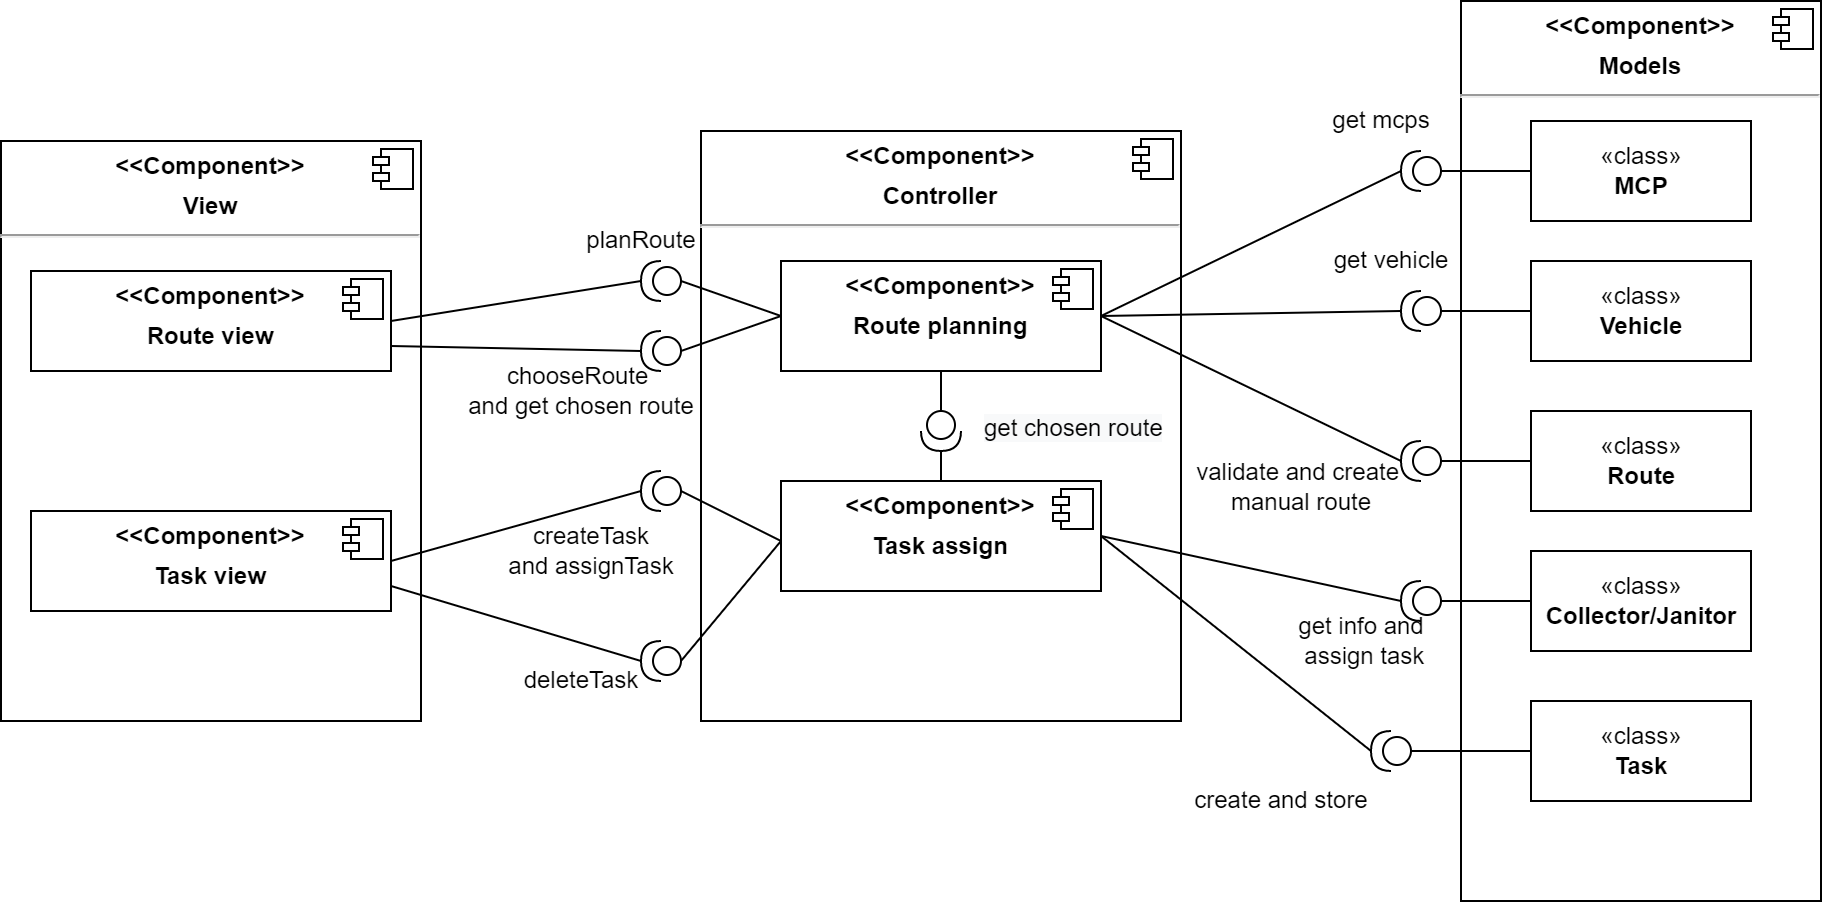
\includegraphics[width=1\linewidth]{imgs/component diagram/component Task Assignment.png}
            \caption{Component diagram cho task assignment module}
        \end{figure}
        Component diagram Task Asignment module gồm 5 Component với luồng thực thi:
        \begin{enumerate}
            \item Đưa dữ liệu Vehicle và MCPs vào Component Planning route và trả về tuyến đường khả dụng.
            \item Đưa dữ liệu các tuyến đường khả dụng vào component Choose route và trả về tuyến đường đã được Back Officer chọn.
            \item Đưa tuyến đường được chọn và Task vào Component Assign route, dữ liệu trả về là Task đã được Assign route.
            \item Đưa dữ liệu Task đã được Assign vào component Schedule time và trả về dữ liệu là Task được định thời gian thực hiện.
            \item Đưa lịch làm đã xếp và Worker vào component Assign staff và trả về kết quả là Task đã được Assign Worker, vehicle, route, calendar.
        \end{enumerate}
    \subsection{Component Diagram cho Planning Route }
        \begin{figure}[h]
            \centering
            \includegraphics[width=1\linewidth]{imgs/Component diagram/Component planning route.png}
            \caption{Component diagram cho Planning Route}
        \end{figure}
        Component diagram cho Planning Route gồm 2 Component thừa kế Component Modification Method với luồn thực thi:
        \begin{itemize}
            \item Auto generate route:
            \begin{enumerate}
                \item Đưa dữ liệu Vehicle, MCPs vào Component Get Avaiable Paths và trả về tuyến đường khả thi.
                \item Đưa dữ liệu các tuyến đường khả dụng vào Component Generate routes and Efficiency Statistic và trả về kết quả là tuyến đường hiệu quả để sử dụng.
            \end{enumerate}

            \item Manual generate route:
            \begin{enumerate}
                \item Đưa dữ liệu tuyến đường vào Component Validate Routes để kiểm thử và trả về tuyến đường đã được kiểm tra.
                \item Đưa tuyến đường đã được kiểm tra vào Component Generate routes and Efficiency Statistic và trả về kết quả là tuyến đường hiệu quả để sử dụng.
            \end{enumerate}
        \end{itemize}
       
       


\end{document}


\documentclass[a4paper]{article}
\usepackage{amssymb,epsfig,latexsym,multicol,array,hhline,fancyhdr}
\usepackage{vntex}
\usepackage{xcolor}
\usepackage{titlesec}
\usepackage{mdframed}
\usepackage{amsmath}
\usepackage{lastpage}
\usepackage[lined,boxed,commentsnumbered]{algorithm2e}
\usepackage{enumerate}
\usepackage{color}
\usepackage[most]{tcolorbox}
\usepackage{graphicx}
\usepackage{array}
\usepackage{float}
\usepackage{tabularx, caption}
\usepackage{tabularray}
\usepackage{colortbl}
\usepackage{longtable}
\usepackage{multirow} 
\usepackage{multicol}
\usepackage{rotating}
\usepackage{graphics}
\usepackage{geometry}
\usepackage{setspace}
\usepackage{epsfig}
\usepackage{wrapfig}
\usepackage{tikz}
\usepackage[most]{tcolorbox}
\usepackage{hyperref}
\usepackage{cleveref}
\usepackage{setspace}
\usepackage{subfiles}
\usepackage{indentfirst}

\hypersetup{urlcolor=blue,linkcolor=black,citecolor=black,colorlinks=true} 
\usetikzlibrary{arrows,snakes,backgrounds}

\newtheorem{theorem}{{\bf Theorem}}
\newtheorem{property}{{\bf Property}}
\newtheorem{proposition}{{\bf Proposition}}
\newtheorem{corollary}[proposition]{{\bf Corollary}}
\newtheorem{lemma}[proposition]{{\bf Lemma}}

\AtBeginDocument{\renewcommand*\contentsname{Nội dung}}
\AtBeginDocument{\renewcommand*\refname{Tham khảo}}
\setlength{\headheight}{40pt}
\pagestyle{fancy}

\fancyhead{}
\fancyhead[L]{
 \begin{tabular}{rl}
    \begin{picture}(25,15)(0,0)
    \put(0,-8){
\includegraphics[width=8mm, height=8mm]{imgs/hcmut.png}}
    %\put(0,-8){\epsfig{width=10mm,figure=hcmut.eps}}
   \end{picture}&
	%
\includegraphics[width=8mm, height=8mm]{hcmut.png} & %
	\begin{tabular}{l}
		\textbf{\bf \ttfamily Đại học Bách Khoa Thành phố Hồ Chí Minh}\\
		\textbf{\bf \ttfamily Khoa Khoa học và Kỹ thuật Máy tính}
	\end{tabular} 	
 \end{tabular}
}
\fancyhead[R]{
	\begin{tabular}{l}
		\tiny \bf \\
		\tiny \bf 
	\end{tabular} 
}
\fancyfoot{} 
\fancyfoot[L]{\scriptsize \ttfamily Bài tập lớn môn Công nghệ phần mềm - Năm học 2022-2023}
\fancyfoot[R]{\scriptsize \ttfamily Trang {\thepage}/\pageref{LastPage}}

\renewcommand{\headrulewidth}{0.3pt}
\renewcommand{\footrulewidth}{0.3pt}


%%%
\setcounter{secnumdepth}{4}
\setcounter{tocdepth}{3}
\makeatletter
\newcounter {subsubsubsection}[subsubsection]
\renewcommand\thesubsubsubsection{\thesubsubsection .\@alph\c@subsubsubsection}
\newcommand\subsubsubsection{\@startsection{subsubsubsection}{4}{\z@}%
                                     {-3.25ex\@plus -1ex \@minus -.2ex}%
                                     {1.5ex \@plus .2ex}%
                                     {\normalfont\normalsize\bfseries}}
\newcommand*\l@subsubsubsection{\@dottedtocline{3}{10.0em}{4.1em}}
\newcommand*{\subsubsubsectionmark}[1]{}
\makeatother


\begin{document}

	\begin{titlepage}
    \begin{center}
        ĐẠI HỌC QUỐC GIA THÀNH PHỐ HỒ CHÍ MINH\\
        TRƯỜNG ĐẠI HỌC BÁCH KHOA \\
        KHOA KHOA HỌC VÀ KỸ THUẬT MÁY TÍNH
    \end{center}

    \vspace{0.4cm}

    \begin{figure}[h!]
        \begin{center}
        
\includegraphics[width=4.5cm]{imgs/hcmut.png}
        \end{center}
    \end{figure}

    \vspace{0.1cm}


    \begin{center}
        \begin{tabular}{c}
        \textbf{{ \Large CÔNG NGHỆ PHẦN MỀM (CO3001)}}\\
        ~~\\
        \hline
        \\
        \multicolumn{1}{l}{\textbf{{\Large Bài tập lớn}}}\\
        \\
        \textbf{\Huge \color{red} URBAN WASTE COLLECTION}\\\\
        \textbf{\Huge \color{red} AID - UWC 2.0}\\
        \\
        \hline
        \end{tabular}
    \end{center}

    \vspace{0.5cm}

    \begin{table}[h]
        \begin{tabular}{rrl}
            \hspace{5 cm} & GVHD: & Lê Đình Thuận.\\
            & Lớp: & L04\_ Nhóm: Tình Đồng Chí \\
            & Sinh viên thực hiện: & Lê Nguyễn Huyền Thoại – 2012122.\\
            & & Trương Huy Thái – 2012036.\\
            & & Nguyễn Tiến Nam – 2011652.\\
            & & Nguyễn Trọng Đức Huy – 2011283.\\
            & & Nguyễn Trọng Nhân – 2011744.\\
            & & Trần Tuấn Anh – 2010878.\\
            & & Phan Thị Quỳnh Như – 2011780. \\
        \end{tabular}
    \end{table}

    \vspace{0.3CM}

    \begin{center}
        {\footnotesize THÀNH PHỐ HỒ CHÍ MINH, THÁNG \the\month /\the\year}
    \end{center}
\end{titlepage}


	\newpage
	\tableofcontents

	\newpage
	\section{Danh sách thành viên \& Khối lượng công việc}

\begin{tblr}{
    width=1\linewidth,
    hlines,
    vlines,
    colspec={X[-2]X[4]X[1.5]X[6]X[-1]},
    columns = {valign = m, },
    column{1} = {halign = c, },
    row{1} = {halign = c, valign = m, bg = lightgray, fg = black},
}
    {\textbf{STT} & \textbf{Họ và tên} & \textbf{MSSV} & \textbf{Công việc} & \textbf{Hoàn thành} }  \\
    1 & Lê Nguyễn Huyền Thoại & 2012122 & - Quản lý tiến độ công việc \newline
                                          - Thiểt kế use-case diagram tổng \newline
                                          - Thiệt kế class diagram \newline
                                          - Thiết kế component diagram
                                        & 100\% \\
    2 & Trương Huy Thái       & 2012036 & - Xác định yêu cầu phi chức năng \newline
                                          - Thiết kế use-case diagram task assignment \newline
                                          - Thiết kế activity diagram  \newline
                                          - Thiết kế architecture design
                                        & 100\% \\
    3 & Nguyễn Tiến Nam		  & 2011652 & - Xác định yêu cầu chức năng \newline
                                          - Viết đặc tả use-case tổng \newline
                                          - Thiết kế class diagram \newline
                                          - Thiết kế architecture design
                                        & 100\% \\
    4 & Nguyễn Trọng Đức Huy  & 2011283 & - Xác định ngữ cảnh dự án \newline
                                          - Thiết kế use-case manage resources \newline
                                          - Thiết kế sequence diagram \newline
                                          - Đánh giá Architecture design
                                        & 100\% \\
    5 & Nguyễn Trọng Nhân     & 2011744 & - Xác định ngữ cảnh dự án \newline
                                          - Viết đặc tả use-case task assignment \newline
                                          - Thiết kế sequence diagram \newline
                                          - Thiết kế component diagram
                                        & 100\% \\
    6 & Trần Tuấn Anh         & 2010878 & - Xác định yêu cầu phi chức năng \newline
                                          - Đánh giá các use-case diagram \newline
                                          - Thiết kế activity diagram \newline
                                          - Đánh giá component diagram
                                        & 100\% \\
    7 & Phan Thị Quỳnh Như    & 2011780 & - Xác định yêu cầu chức năng \newline
                                          - Đánh giá activity diagram, sequence diagram, class diagram \newline
                                          - Đánh giá tổng quan task 3 \newline
                                          - Viết báo cáo
                                        & 100\% \\

\end{tblr}


	%%%%%%%%%%%%%%%%%%%%%%%%%%%%%%%%%


	%%%%%%%%%%%%%%%%%%%%%%%%%%%%%%%%%
	\newpage
	\subsection{Mô tả chung}
    \quad Sau đại dịch covid-19, sức khỏe đã và đang là một trong những vấn đề được nhiều người quan tâm. Nhận thấy được vấn đề này, nhóm muốn tạo ra một ứng dụng nhằm nâng cao sức khỏe của người sử dụng bằng việc đưa ra những món ăn phù hợp với mục tiêu nhu cầu của từng người. Ví dụ như người dùng muốn tăng cân, tăng cơ, phần mềm sẽ đưa ra các món ăn làm sao để trong một khoảng thời gian nhất định, người dùng có thể đạt được cân nặng mà họ mong muốn. Ngoài ra nó còn cung cấp cho người dùng một lượng lớn các công thức nấu ăn đơn giản mà vẫn ngon miệng, phù hợp với cuộc sống ngày càng nhanh hiện nay.\\
    
    \begin{figure}[h]
        \centering
        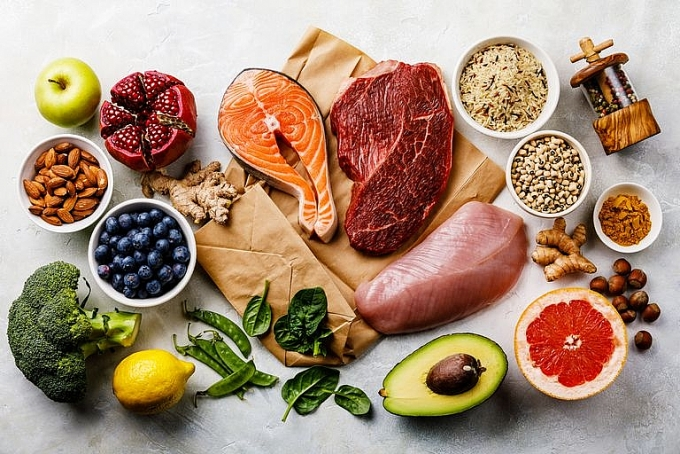
\includegraphics[width=0.7\linewidth]{images/healthy-food.jpg}
        \caption{Các chất có trong bữa ăn}
    \end{figure}
\section{Xác định ngữ cảnh của dự án UWC 2.0}
    \subsection{Các bên liên quan (Relevant Stakeholders)}
        \begin{enumerate}
            \item Công ty cung cấp dịch vụ thu dọn rác Y, ở vai trò là người quản lý.
            \item Công ty cung cấp dịch vụ thu dọn rác Y, ở vị trí là người sở hữu phần mềm UWC 2.0.
            \item Tổ chức X, phát triển phần mềm UWC 2.0.
            \item Công nhân sử dụng phần mềm UWC 2.0.
            \item Các bên liên quan khác (chính phủ, người dân).
        \end{enumerate}
    
    \subsection{Những mong muốn của các bên liên quan}
        \begin{enumerate}
            \item Công ty cung cấp dịch vụ thu dọn rác Y, ở vai trò là người quản lý, họ mong muốn phần mềm UWC 2.0 sẽ mang lại cho công ty:
            \begin{itemize}
                \item[-] Khả năng quản lý nhân lực, kiểm tra một cách hiệu quả cũng như thường xuyên cập nhật thông tin về sức chứa của các điểm tập trung rác thải (MCPs) và những thông tin nhằm phục vụ nhu cầu bảo trì các phương tiện vận chuyển, trang thiết bị của công ty.
                \item[-] Nâng cao hiệu suất thu gom rác thải của công ty.
                \item[-] Hệ thống khi được đưa vào hoạt động có độ tin cậy cao, hoạt động tốt trong mọi tình huống.
            \end{itemize}
            
            \item Công ty cung cấp dịch vụ thu dọn rác Y, ở vị trí là người sở hữu phần mềm UWC 2.0, họ sẽ có những mong muốn:
            \begin{itemize}
                \item[-] Khả năng mở rộng phạm vi hoạt động của hệ thống, không chỉ là trong một vùng, một quận cố định, mà có thể xử lý trong phạm vi toàn thành phố.
                \item[-] Chi phí và lợi nhuận luôn là một trong những vấn đề ưu tiên hàng đầu cần phải được cân nhắc. Khi được đưa vào sử dụng, UWC 2.0 phải đảm bảo tối ưu hóa về mặt nhiên liệu để từ đó giảm thiểu được chi phí phải bỏ ra. Thêm vào đó là chi phí để bảo trì hệ thống cũng phải phù hợp với công ty.
                \item[-] Trước đây công ty đã có sẵn hệ thống UWC 1.0 và công ty mong muốn có thể tận dụng lại tối đa dữ liệu có sẵn từ phiên bản trước và khả năng tương thích ngược giữa phiên bản 1.0 và 2.0.
                \item[-] Đem lại những kết quả tích cực đến công tác xử lý và tái chế rác thải trong cộng đồng, tạo ra môi trường sống xanh, sạch, đẹp cho người dân.
            \end{itemize}
      
            \item Tổ chức X, phát triển phần mềm UWC 2.0 có mong muốn:
            \begin{itemize}
                \item[-] Xây dựng được hệ thống có thể làm được và làm tốt những yêu cầu tối thiểu được yêu cầu bởi công ty chủ quản, xa hơn nữa là hoàn thiện hệ thống một cách tối ưu.
                \item[-] Hệ thống khi đến tay khách hàng phải dễ dàng bảo dưỡng, để nếu trong tương lai nếu khách hàng có thuê một công ty khác sửa chữa, bảo dưỡng hệ thống cũng thuận tiện hơn.
            \end{itemize}
        
            \item Công nhân sử dụng phần mềm UWC 2.0 mong muốn:
            \begin{itemize}
                \item[-] Vì đa phần người dùng là các cô chú trung niên, lớn tuổi, phần mềm nên có giao diện thân thiện, dễ dàng tiếp cận và làm quen.
                \item[-] Có thể sử dụng phần mềm trên nhiều thiết bị khác nhau như máy tính, điện thoại hay máy tính bảng.
                \item[-] Phần mềm phải sử dụng ổn định, ít giật lag và độ tin cậy cao.
            \end{itemize}
       
            \item Các bên liên quan khác (chính phủ, người dân): mong muốn phần mềm sẽ mang lại những ảnh hưởng tích cực đến công tác quản lý và tái sử dụng rác thải trong phạm vi khu vực và trong cả nước.
        \end{enumerate}
    
    \subsection{Vấn đề các bên liên quan đang gặp phải}
        \begin{enumerate}
            \item Công ty cung cấp dịch vụ thu dọn rác Y hiện đang gặp phải các vấn đề:
            \begin{itemize}
                \item[-] Công ty đang thiếu khả năng kiểm tra tình trạng trang thiết bị và phương tiện nên việc hoạt động chưa hiệu quả.
                \\
                \emph{\underline{Ví dụ}}: Chưa kiểm soát được tải trọng, sức chứa, tiêu thụ nhiên liệu dẫn tới sự phân bố xe chưa hợp lý khi hoạt động.
                
                \item[-] Việc quản lý nhân lực của công ty chưa hiệu quả:
                \begin{itemize}
                    \item[+] Công ty chưa theo dõi được tiến độ làm việc, hiệu suất làm việc của nhân viên.
                    \item[+] Việc phân công công việc chưa hợp lý gây mất công bằng và giảm hiệu suất công việc.
                \end{itemize}
            \end{itemize}
            
            \item Công ty cung cấp dịch vụ thu dọn rác Y, ở vị trí là người sở hữu hệ thống đang gặp phải các vấn đề:
            \begin{itemize}
                \item[-] Khả năng duy trì và nâng cấp hệ thống. Việc duy trì hệ thống đang có chi phí cao, chưa hợp lý.
                \item[-] Khi gặp các sự cố bất ngờ như  tai nạn, hư hỏng thiết bị thì việc liên lạc để điều phối nhân viên chưa kịp thời .
                \item[-] Công ty gặp bất tiện trong việc theo dõi và phân công lịch trình: lịch trình giấy, phân công thủ công. Điều này khiến công ty mất nhiều thời gian, nhân sự và việc phân công này chưa được tối ưu.
            \end{itemize}
            
            \item Các bên liên quan khác (chính phủ, người dân): Việc cải thiện môi trường chưa được tối ưu hoá, chi phí cao nhưng chưa hiệu quả dẫn đến lãng phí.
        \end{enumerate}
    
    \subsection{Lợi ích mà các bên liên quan có thể đạt được khi sử dụng hệ thống UWC 2.0}
        \begin{enumerate}
            \item Nhà cung cấp dịch vụ thu dọn rác Y ở vai trò quản lý:
            \begin{itemize}
                \item[-] Nắm bắt được cụ thể tình trạng hiện tại của các trang thiết bị và cơ sở vật chất, từ đó có thể đưa ra được những quyết định như nâng cấp, sửa chữa hay bổ sung trang thiết bị cho công nhân một cách kịp thời và hiệu quả.
                \item[-] Nhanh chóng theo dõi được tiến độ, hiệu suất làm việc của nhân viên. Đưa ra được phương án giải quyết sự cố kịp thời và công bằng.
            \end{itemize}
    
            \item Nhà cung cấp dịch vụ Y dưới góc độ chủ sở hữu hệ thống:
            \begin{itemize}
                \item[-] Tiết kiệm được chi phí duy trì và phát triển hệ thống.
                \item[-] Mang lại danh tiếng cho công ty trong mảng thu dọn rác thải.
            \end{itemize}
    
            \item Tổ chức X qua vai trò nhà phát triển phần mềm:
            \begin{itemize}
                \item[-] Tăng thu nhập cho công ty cũng như thu nhập của các cá nhân tham gia phát triển hệ thống.
                \item[-] Tăng kỹ năng của từng cá nhân.
                \item[-] Nâng cao danh tiếng, sự tin cậy cho doanh nghiệp.
            \end{itemize}
          
            \item Nhân viên  sử dụng phần mềm:
            \begin{itemize}
                \item[-] Dễ dàng sử dụng và làm quen.
                \item[-] Công sức làm việc của bản thân mỗi người được đánh giá công bằng và rõ ràng.
                \item[-] Khả năng liên lạc nhanh chóng giữa công nhân và nhân viên giám sát nhằm xử lý được những tình huống bất ngờ có thể xảy ra trong quá trình làm việc.
            \end{itemize}
            
            \item Người bị ảnh hưởng khác (chính phủ, người dân): Bảo vệ môi trường.
        \end{enumerate}
    \newpage

\section{Yêu cầu (Requirements)}
    \subsection{Yêu cầu chức năng (Functional)}
        \begin{enumerate}
            \item \textbf{Nhân viên giám sát (Back officer)}
           
            \begin{tblr}{
                width=1\linewidth,
                hlines,
                vlines,
                colspec={X[-1]X[4]X[7]},
                columns = {valign = m, },
                row{1} = {halign = c, valign = m, bg = lightgray, fg = black},
            }
                {\textbf{\#}} & \textbf{Chức năng} & {\textbf{Mô tả}} \\
                1 & Xem thông tin cá nhân & Cho phép xem chi tiết thông tin cá nhân của công nhân.\\
                2 & Xem lịch làm việc &  Xem lịch làm của từng công nhân.\\
                3 & Xem phương tiện & Xem được thông tin của từng phương tiện, các thông số kỹ thuật như trọng lượng, lượng nhiên liệu tiêu thụ, tình trạng, ...\\
                4 & Xem các điểm MCPs & Xem được thông tin các điểm MCPs, dung tích còn lại của nó.\\
                5 & Phân công công việc & Nhân viên giám sát có thể phân công công việc cho từng công nhân bao gồm việc phân phương tiện, gán các điểm MCPs và tạo tuyến đường cho công nhân lái xe rác.\\
                6 & Nhắn tin & Nhân viên giám sát có thể liên lạc với công nhân trong trường hợp bất ngờ xảy ra.\\
                7 & Thay đổi mật khẩu & Cho phép thay đổi mật khẩu trong trường hợp mong muốn hoặc thay đổi mật khẩu và có phương án xác thực dự phòng trong trường hợp quên mật khẩu.\\
                8 & Đăng nhập & Nhân viên giám sát đăng nhập vào tài khoản để sử dụng các tính năng.\\
            \end{tblr}
         
            \item \textbf{Người quản lý (Administrator)}
           
            \begin{tblr}{
                width=1\linewidth,
                hlines,
                vlines,
                colspec={X[-1]X[4]X[7]},
                columns = {valign = m, },
                row{1} = {halign = c, valign = m, bg = lightgray, fg = black},
            }
                {\textbf{\#}} & \textbf{Chức năng} & {\textbf{Mô tả}} \\
                1 & Quản lý nhân viên & Cho phép tạo, sửa, xóa một nhân viên trong hệ thống.\\
                2 & Quản lý phương tiện & Cho phép thêm, sửa, xóa một phương tiện trong hệ thống.\\
                3 & Quản lý các MCPs & Cho phép thêm, sửa, xóa các MCPs.\\
                4 & Thay đổi mật khẩu & Cho phép thay đổi mật khẩu trong trường hợp mong muốn hoặc thay đổi mật khẩu và có phương án xác thực dự phòng trong trường hợp quên mật khẩu.\\
                5 & Đăng nhập & Quản lý đăng nhập vào tài khoản để sử dụng các tính năng.\\
            \end{tblr}
           
            \newpage
            \item \textbf{Công nhân (Janitor / Collector)}
           
            \begin{tblr}{
                width=1\linewidth,
                hlines,
                vlines,
                colspec={X[-1]X[4]X[7]},
                columns = {valign = m, },
                row{1} = {halign = c, valign = m, bg = lightgray, fg = black},
            }
                {\textbf{\#}} & \textbf{Chức năng} & {\textbf{Mô tả}} \\
                1 & Xem thông tin cá nhân & Cho phép xem chi tiết thông tin cá nhân của công nhân.\\
                2 & Xem lịch làm việc & Cho phép công nhân xem lịch làm việc cụ thể trong từng ngày và tổng quát ở mỗi tuần.\\
                3 & Check in / check out & Công nhân xác nhận công việc trong ngày và đánh dấu hoàn thành công việc mỗi ngày.\\
                4 & Nhắn tin & Công nhân có thể liên lạc với văn phòng trong trường hợp bất ngờ xảy ra.\\
                5 & Nhận thông báo & Nhận thông báo mỗi khi lịch làm việc được giao cũng như tình trạng của MCPs. \\
                6 & Thay đổi mật khẩu & Cho phép thay đổi mật khẩu trong trường hợp mong muốn hoặc thay đổi mật khẩu và có phương án xác thực dự phòng trong trường hợp quên mật khẩu.\\
                7 & Đăng nhập & Công nhân đăng nhập vào tài khoản để sử dụng các tính năng.\\
            \end{tblr}
        \end{enumerate}
   
    \subsection{Yêu cầu phi chức năng (Non-functional)}
        \begin{enumerate}
            \item \textbf{Thiết kế giao diện người dùng (UI design)}
           
            \begin{tblr}{
                width=1\linewidth,
                hlines,
                vlines,
                colspec={X[-1]X[11]},
                columns = {valign = m, },
                row{1} = {halign = c, valign = m, bg = lightgray, fg = black},
            }
                {\textbf{\#}} & \textbf{Yêu cầu} \\
                1 & Thông tin quan trọng nên được hiển thị trong một lần xem (không cần kéo xuống). \\
                2 & Giao diện đơn giản. Có thể tự tìm hiểu cách sử dụng không cần hướng dẫn trong 15 phút. \\
                3 & Giao diện hệ thống: tiếng Việt và tiếng Anh cho tương lai.\\
            \end{tblr}
           
            \item \textbf{Hiệu suất (Performance)}
           
            \begin{tblr}{
                width=1\linewidth,
                hlines,
                vlines,
                colspec={X[-1]X[11]},
                columns = {valign = m, },
                row{1} = {halign = c, valign = m, bg = lightgray, fg = black},
            }
                {\textbf{\#}} & \textbf{Yêu cầu} \\
                1 & Xử lý thời gian thực với ít nhất 1000 MCPs trong thời điểm hiện tại và 10000 MCPs trong 5 năm tới.\\
                2 & Sức chứa của MCPs cần được cập nhật mỗi 15 phút. \\
                3 & Độ trễ giao tiếp thời gian thực ở dưới 1 giây. \\
                4 & Thời gian gợi ý tuyến đường tối ưu dưới 10 giây. \\
                5 & Thời gian lấy dữ liệu của công nhân dưới 5 giây. \\
            \end{tblr}
           
            \newpage
            \item \textbf{Tương thích (Compatibility)}
           
            \begin{tblr}{
                width=1\linewidth,
                hlines,
                vlines,
                colspec={X[-1]X[11]},
                columns = {valign = m, },
                row{1} = {halign = c, valign = m, bg = lightgray, fg = black},
            }
                {\textbf{\#}} & \textbf{Yêu cầu} \\
                1 & Có thể lấy và sử dụng dữ liệu cũ từ UWC 1.0.\\
                2 & Hoạt động tương thích với UWC 1.0 \\
            \end{tblr}
           
            \item \textbf{Nền tảng (Platform)}
           
            \begin{tblr}{
                width=1\linewidth,
                hlines,
                vlines,
                colspec={X[-1]X[11]},
                columns = {valign = m, },
                row{1} = {halign = c, valign = m, bg = lightgray, fg = black},
            }
                {\textbf{\#}} & \textbf{Yêu cầu} \\
                1 & Là ứng dụng web, có thể cải tiến cho ứng dụng di động trong tương lai. \\
            \end{tblr}
        \end{enumerate}
    \newpage

\section{Use-case diagram}
    

\subsection{Tổng quát của hệ thống}
    \begin{figure}[h]
        \centering
        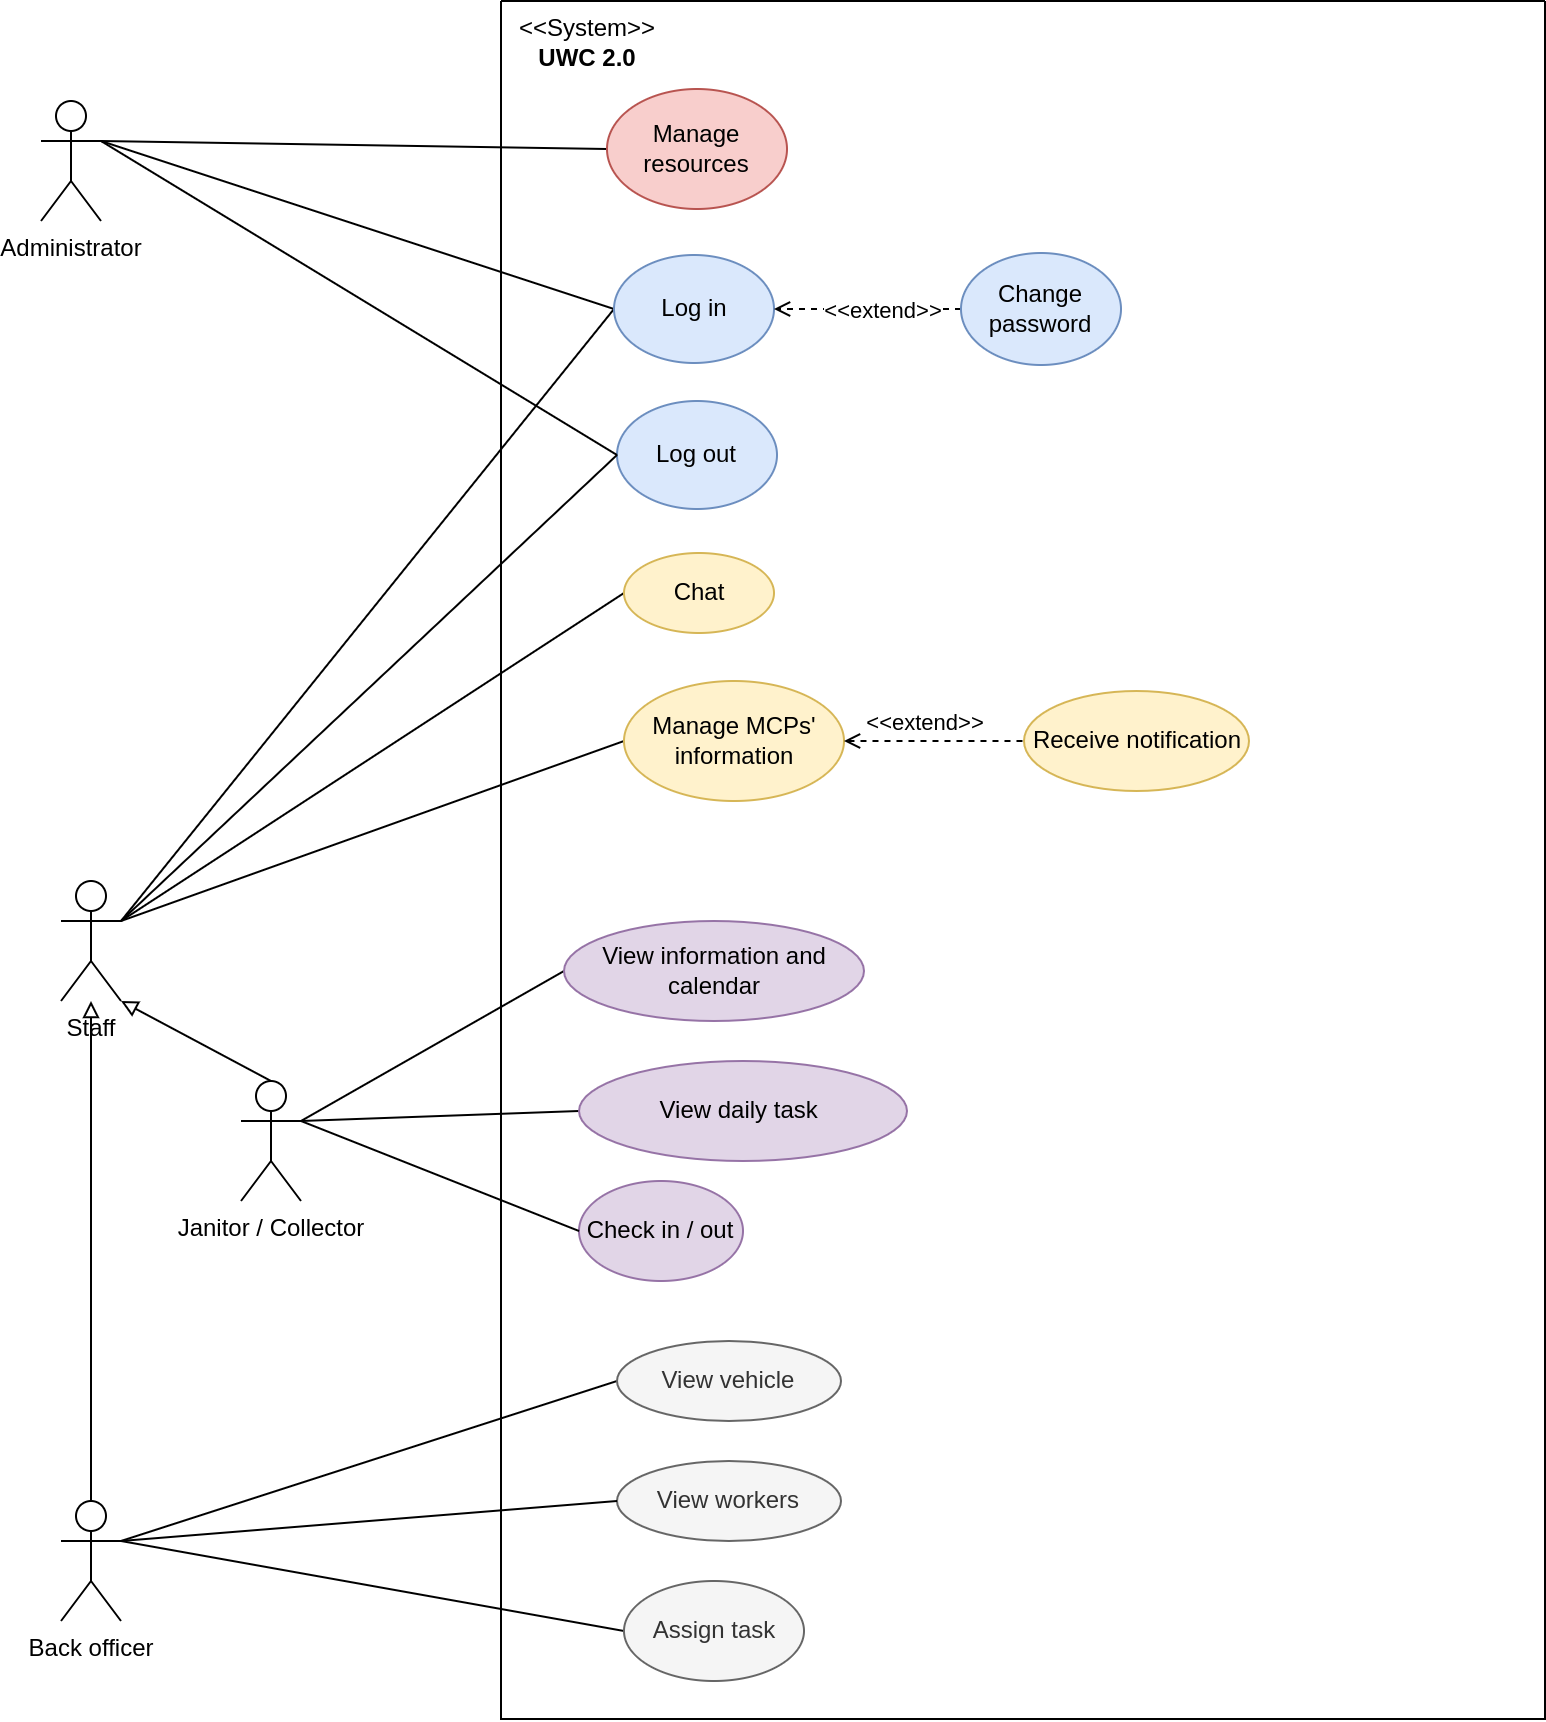
\includegraphics[width=0.93\linewidth]{imgs/use-case diagram/main_uc.png}
        \caption{Use-case diagram tổng quát của hệ thống}
    \end{figure}

    \begin{tblr}{
        width=1\linewidth,
        hlines,
        vlines,
        colspec={X[3]X[7]},
        columns = {valign = m, },
        row{1} = {halign = c, valign = m, bg = lightgray, fg = black},
    }
        {\textbf{Use case name} & \textbf{Manage resources}}  \\
        Description	& Quản lý tài nguyên của công ty \\
        Actor & Người quản lý (Administrator) \\
        Trigger & Người quản lý ấn vào phần quản lý tài nguyên  \\
        Pre-condition & Người quản lý đã đăng nhập và đang ở màn hình chính\\
        Post-condition & Người quản lý được đưa vào trang quản lý tài nguyên\\
        Normal flow &   		1. Hệ thống hiển thị giao diện quản lý tài nguyên \newline
                                2. Quản lý thực hiện việc quản lý tài nguyên \\
        Alternative flow  & 	none \\
        Exception flow & none\\
    \end{tblr}

    \vspace{1cm}

    \begin{tblr}{
        width=1\linewidth,
        hlines,
        vlines,
        colspec={X[3]X[7]},
        columns = {valign = m, },
        row{1} = {halign = c, valign = m, bg = lightgray, fg = black},
    }
        {\textbf{Use case name} & \textbf{Log in}}  \\
        Description	& Đăng nhập vào hệ thống \\
        Actor & Người quản lý (Administrator), nhân viên giám sát (Back officer), nhân viên lái xe rác (Collector), nhân viên thu gom rác (Janitor) \\
        Trigger & Người dùng mở ứng dụng  \\
        Pre-condition & Thiết bị phải có kết nối Internet\\
        Post-condition & Người dùng đăng nhập thành công\\
        Normal flow &   1. Hệ thống hiển thị giao diện đăng nhập \newline
                    	2. Người dùng ghi thông tin về tên tài khoản và mật khẩu \newline
                    	3. Hệ thống kiểm tra thông tin được ghi \newline
                    	4. Hệ thống thông báo đăng nhập thành công \newline
                    	5. Hệ thống hiển thị giao diện màn hình chính \\
        Alternative flow  & Alternative flow thứ 1: tại bước 2 \newline
                        	1a. Người dùng chọn lưu tài khoản \newline
                        	Tiếp tục bước 3 \newline
                        	1b. Hệ thống lưu lại tài khoản \newline
                        	Tiếp tục bước 4 \\
        Exception flow & 	Exception flow thứ 1: tại bước 3 \newline
                        	1a. Nếu không tìm thấy tài khoản, sai mật khẩu, thông báo cho người dùng \newline
                        	Quay lại bước 2 \\
        Extended points & Change password \\
    \end{tblr}

    \vspace{1cm}
    \begin{tblr}{
        width=1\linewidth,
        hlines,
        vlines,
        colspec={X[3]X[7]},
        columns = {valign = m, },
        row{1} = {halign = c, valign = m, bg = lightgray, fg = black},
    }
        {\textbf{Use case name} & \textbf{Change password}}  \\
        Description	& Thay đổi mật khẩu của tài khoản \\
        Actor & Người quản lý (Administrator), nhân viên giám sát (Back officer), nhân viên lái xe rác (Collector), nhân viên thu gom rác (Janitor) \\
        Trigger & Người dùng ấn vào nút quên mật khẩu  \\
        Pre-condition & Người dùng đang ở phần đăng nhập \\
        Post-condition & Mật khẩu được thay đổi thành công \\
        Normal flow &   1. Hệ thống hiển thị thay giao diện thay đổi mật khẩu \newline
                    	2. Người dùng nhập tên tài khoản \newline
                    	3. Hệ thống kiểm tra tài khoản \newline
                    	4. Người dùng nhập mã mật khẩu mới \newline
                    	5. Hệ thống kiểm tra mật khẩu mới \newline
                    	6. Hệ thống thông báo đổi mật khẩu thành công \newline
                    	7. Hệ thống quay lại trang đăng nhập \\
        Alternative flow  & none \\
        Exception flow & 	Exception flow thứ 1: tại bước 3 \newline
                            1a. Nếu tài khoản không tồn tại, thông báo cho người dùng \newline
                            Quay lại bước 2 \newline

                            Exception flow thứ 2: tại bước 5 \newline
                            2a. Nếu mật khẩu không đúng quy đinh, thông báo cho người dùng \newline
                            Quay lại bước 4 \\
    \end{tblr}

    \vspace{1cm}
    \begin{tblr}{
        width=1\linewidth,
        hlines,
        vlines,
        colspec={X[3]X[7]},
        columns = {valign = m, },
        row{1} = {halign = c, valign = m, bg = lightgray, fg = black},
    }
        {\textbf{Use case name} & \textbf{Log out}}  \\
        Description	& Đăng xuất khỏi phiên làm việc \\
        Actor & Người quản lý (Administrator), nhân viên giám sát (Back officer), nhân viên lái xe rác (Collector), nhân viên thu gom rác (Janitor) \\
        Trigger & Người dùng ấn vào nút đăng xuất  \\
        Pre-condition & Người dùng đã đăng nhập, và đang ở màn hình chính \\
        Post-condition & Tài khoản được đăng xuất khỏi hệ thống \\
        Normal flow &   1. Người dùng ấn vào menu \newline
                    	2. Người dùng chọn đăng xuất \newline
                    	3. Hệ thống hiện thị form xác nhận đăng xuất \newline
                    	4. Hệ thống xóa phiên làm việc  \newline
                    	5. Hệ thống quay trở lại trang đăng nhập \\
        Alternative flow  & Alternative flow thứ 1: tại bước 3 \newline
                            1a. Nếu người dùng chọn hủy, quay lại màn hình chính \\
        Exception flow & none\\
    \end{tblr}

    \begin{tblr}{
        width=1\linewidth,
        hlines,
        vlines,
        colspec={X[3]X[7]},
        columns = {valign = m, },
        row{1} = {halign = c, valign = m, bg = lightgray, fg = black},
    }
        {\textbf{Use case name} & \textbf{Chat}}  \\
        Description	& Nhân viên liên lạc với nhau \\
        Actor & Nhân viên (Staff) \\
        Trigger & 	Nhân viên ấn vào phần liên hệ \\
        Pre-condition & Người dùng đã đăng nhập\\
        Post-condition & Tin nhắn được gửi thành công \newline
                         Nhân viên nhận và đọc được tin nhắn \\
        Normal flow &   1. Hệ thống lấy thông tin về các nhân viên \newline
                    	2. Hệ thống hiển thị danh sách các nhân viên \newline
                    	3. Người dùng chọn nhân viên muốn liên hệ \newline
                    	4. Hệ thống hiển thị giao diện nhắn tin \newline
                    	5. Người dùng nhập tin nhắn \newline
                    	6. Người dùng nhấn gửi \newline
                    	7. Hệ thống ghi nhận tin nhắn và gửi cho người được nhắn \\
        Alternative flow  & none \\
        Exception flow & none \\
    \end{tblr}

    \vspace{1cm}
    \begin{tblr}{
        width=1\linewidth,
        hlines,
        vlines,
        colspec={X[3]X[7]},
        columns = {valign = m, },
        row{1} = {halign = c, valign = m, bg = lightgray, fg = black},
    }
        {\textbf{Use case name} & \textbf{Manage MCP's information}}  \\
        Description	& Xem thông tin về các MCPs \\
        Actor & Nhân viên (Staff) \\
        Trigger & 	Nhân viên ấn vào mục tổng quan MCPs \\
        Pre-condition & Nhân viên đã đăng nhập và đang ở màn hình chính \\
        Post-condition & Thông tin về MCP được hiển thị thành công \\
        Normal flow &   1. Hệ thống lấy thông tin các MCPs \newline
                    	2. Hệ thống hiện thị danh sách các MCPs \newline
                    	3. Nhân viên chọn 1 MCP bất kì \newline
                    	4. Hệ thống hiển thị thông tin chi tiết của MCPs vừa được chọn \\
        Alternative flow  & none \\
        Exception flow & none \\
        Extended points & Receive notification \\
    \end{tblr}

    \begin{tblr}{
        width=1\linewidth,
        hlines,
        vlines,
        colspec={X[3]X[7]},
        columns = {valign = m, },
        row{1} = {halign = c, valign = m, bg = lightgray, fg = black},
    }
        {\textbf{Use case name} & \textbf{Receive notification}}  \\
        Description	& Cập nhật tình trạng của MCP \\
        Actor & Nhân viên (Staff) \\
        Trigger & none \\
        Pre-condition & Nhân viên đã đăng nhập \\
        Post-condition & Thông báo được nhận bởi nhân viên \\
        Normal flow &   1. Hệ thống truy cập vào dữ liệu về MCPs \newline
                    	2. Hệ thống lấy thông tin về dung tích của MCPs \newline
                    	3. Hệ thống gửi thông báo về cho người dùng \newline
                    	4. Người dùng nhận được thông báo \\
        Alternative flow  & none \\
        Exception flow & none \\
    \end{tblr}

    \vspace{1cm}
    \begin{tblr}{
        width=1\linewidth,
        hlines,
        vlines,
        colspec={X[3]X[7]},
        columns = {valign = m, },
        row{1} = {halign = c, valign = m, bg = lightgray, fg = black},
    }
        {\textbf{Use case name} & \textbf{View information and calendar}}  \\
        Description	& Công nhân xem thông tin và lịch làm trong tuần \\
        Actor & 	Nhân viên lái xe rác (Collector), Nhân viên thu gom rác (Janitor) \\
        Trigger & 	Công nhân ấn vào phần thông tin và lịch làm \\
        Pre-condition & Công nhân đã đăng nhập và đang ở màn hình chính \\
        Post-condition & Công nhân xem được thông tin và lịch làm của mình \\
        Normal flow &   1. Hệ thống lấy thông tin và lịch làm \newline
                    	2. Hệ thống hiển thị giao diện bao gồm 2 tab (thông tin chung, lịch làm) 	mặc định ở thông tin chung \newline
                    	3. Công nhân xem thông tin của bản thân\\
        Alternative flow  & Alternative flow thứ 1: Tại bước 2 \newline
                    	    1a. Người dùng chọn tab lịch làm \newline
                    	    1b. Hệ thống hiển thị giao diện về lịch làm việc trong tuần \\
        Exception flow & none \\
    \end{tblr}

    \begin{tblr}{
        width=1\linewidth,
        hlines,
        vlines,
        colspec={X[3]X[7]},
        columns = {valign = m, },
        row{1} = {halign = c, valign = m, bg = lightgray, fg = black},
    }
        {\textbf{Use case name} & \textbf{View daily task}}  \\
        Description	& Công nhân xem chi tiết công việc trong ngày \\
        Actor & 	Nhân viên lái xe rác (Collector), Nhân viên thu gom rác (Janitor) \\
        Trigger & 	Công nhân ấn vào phần nhiệm vụ hôm nay\\
        Pre-condition & Công nhân đã đăng nhập và đang ở màn hình chính \\
        Post-condition & Nhiệm vụ cụ thể trong ngày được hiện lên màn hình \\
        Normal flow &   1. Hệ thống lấy thông tin làm việc trong ngày \newline
                    	2. Hệ thống hiển thị thông tin làm việc \newline
                    	3. Người dùng đọc được thông tin làm việc\\
        Alternative flow  & none \\
        Exception flow & none \\
    \end{tblr}

    \vspace{1cm}
    \begin{tblr}{
        width=1\linewidth,
        hlines,
        vlines,
        colspec={X[3]X[7]},
        columns = {valign = m, },
        row{1} = {halign = c, valign = m, bg = lightgray, fg = black},
    }
        {\textbf{Use case name} & \textbf{Check in/out}}  \\
        Description	& Nhận và đánh dấu hoàn thành công việc \\
        Actor & 	Nhân viên lái xe rác (Collector), Nhân viên thu gom rác (Janitor) \\
        Trigger & 		Công nhân chọn nhận công việc \\
        Pre-condition & Công nhân đang ở phần thông tin nhiệm vụ chi tiết \\
        Post-condition & Nhiệm vụ được nhận / được hoàn thành \\
        Normal flow &   1. Công nhân xác nhận nhiệm vụ \newline
                        2. Hệ thống ghi nhận công nhân đã xác nhận \\
        Alternative flow  & Alternative flow thứ 1: tại bước 1 \newline
                        	1a. Công nhân ấn hoàn thành nhiệm vụ \newline
                        	1b. Hệ thống ghi nhận \\
        Exception flow & none \\
    \end{tblr}

    \begin{tblr}{
        width=1\linewidth,
        hlines,
        vlines,
        colspec={X[3]X[7]},
        columns = {valign = m, },
        row{1} = {halign = c, valign = m, bg = lightgray, fg = black},
    }
        {\textbf{Use case name} & \textbf{View workers}}  \\
        Description	& Xem thông tin công nhân và lịch làm của họ \\
        Actor & 	Nhân viên giám sát (Back officer) \\
        Trigger & 	Nhân viên giám sát ấn vào mục quản lý nhân viên \\
        Pre-condition & Nhân viên giám sát đã đăng nhập và đang ở màn hình chính \\
        Post-condition & Thông tin chi tiết và lịch làm việc trong tuần của công nhân được hiển thị \\
        Normal flow &   1. Hệ thống lấy dữ liệu của nhân viên \newline
                    	2. Hệ thống hiển thị danh sách tên các nhân viên \newline
                    	3. Nhân viên giám sát chọn một nhân viên \newline
                    	4. Hệ thống hiển thị thông tin chi tiết của nhân viên \\
        Alternative flow  & Alternative flow thứ 1: tại bước 4 \newline
                        	1a. Người dùng chọn qua mục lịch làm việc \newline
                        	1b. Hệ thống lấy thông tin về lịch làm việc của nhân viên \newline
                        	1c. Hệ thống hiển thị lên màn hình \\
        Exception flow & none \\
    \end{tblr}

    \vspace{1cm}
    \begin{tblr}{
        width=1\linewidth,
        hlines,
        vlines,
        colspec={X[3]X[7]},
        columns = {valign = m, },
        row{1} = {halign = c, valign = m, bg = lightgray, fg = black},
    }
        {\textbf{Use case name} & \textbf{View vehicle}}  \\
        Description	& Xem thông tin của các phương tiện \\
        Actor & 	Nhân viên giám sát (Back officer) \\
        Trigger & 	Nhân viên giám sát ấn vào mục theo dõi phương tiện\\
        Pre-condition & Nhân viên giám sát đã đăng nhập và đang ở màn hình chính \\
        Post-condition & Thông tin phương tiện được hiển thị trên màn hình \\
        Normal flow &   1. Hệ thống truy cập vào dữ liệu về phương tiện \newline
                    	2. Hệ thống hiển thị các phương tiện \newline
                    	3. Người dùng chọn một phương tiện bất kì \newline
                    	4. Hệ thống hiện thị thông tin chi tiết của phương tiện \\
        Alternative flow  & none \\
        Exception flow & none \\
    \end{tblr}
    \newpage

    
\subsection{Chức năng phân chia công việc (Task assignment)}
    \begin{figure}[h]
        \centering
        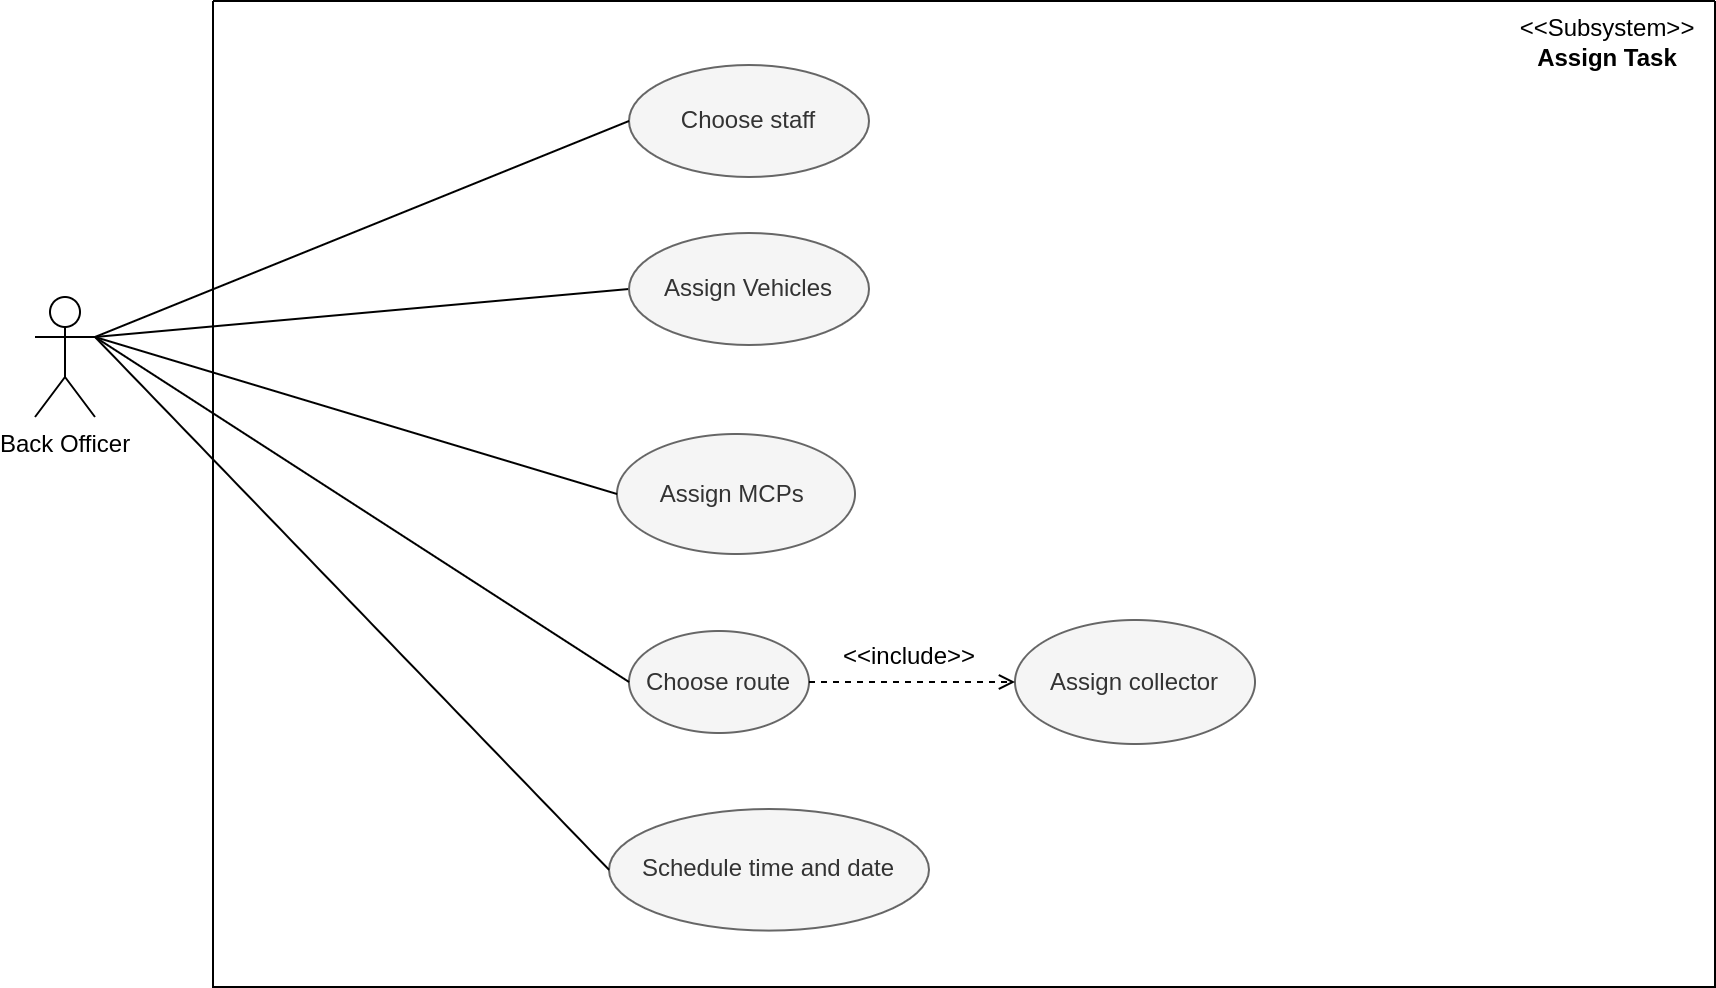
\includegraphics[width=1\linewidth]{imgs/use-case diagram/assignTask_uc.png}
        \caption{Use-case diagram chức năng phân chia công việc}
    \end{figure}

    \vspace{1cm}
    \begin{tblr}{
        width=1\linewidth,
        hlines,
        vlines,
        colspec={X[3]X[7]},
        columns = {valign = m, },
        row{1} = {halign = c, valign = m, bg = lightgray, fg = black},
    }
        {\textbf{Use case name} & \textbf{Choose staff}}  \\
        Description	& Chọn một nhân viên trong hệ thống \\
        Actor & 	Nhân viên giám sát (Back officer) \\
        Trigger & 		Nhân viên giám sát ấn nút chọn công nhân\\
        Pre-condition & Nhân viên giám sát đang ở phần phân công công việc \\
        Post-condition & Công nhân được chọn \\
        Normal flow &   1. Hệ thống lấy dữ liệu về công nhân \newline
                    	2. Hệ thống hiển thị các công nhân \newline
                    	3. Nhân viên giám sát chọn công nhân \newline
                    	4. Hệ thống ghi nhận công nhân được chọn \\
        Alternative flow  & none \\
        Exception flow & none \\
    \end{tblr}

    \begin{tblr}{
        width=1\linewidth,
        hlines,
        vlines,
        colspec={X[3]X[7]},
        columns = {valign = m, },
        row{1} = {halign = c, valign = m, bg = lightgray, fg = black},
    }
        {\textbf{Use case name} & \textbf{Choose vehicle}}  \\
        Description	& Chọn một phương tiện có trong công ty \\
        Actor & 	Nhân viên giám sát (Back officer) \\
        Trigger & 		Nhân viên giám sát ấn nút chọn công nhân\\
        Pre-condition & Nhân viên giám sát đang ở phần phân công công việc \\
        Post-condition & Phương tiện được chọn thành công \\
        Normal flow &   1. Hệ thống lấy dữ liệu về phương tiện \newline
                    	2. Hệ thống hiển thị các phương tiện \newline
                    	3. Nhân viên giám sát chọn phương tiện \newline
                    	4. Hệ thống kiểm tra phương tiện đã được lái hay chưa \newline
                    	5. Hệ thống ghi nhận phương tiện được chọn \\
        Alternative flow  & none \\
        Exception flow & Exception flow thứ 1: tại bước 4 \newline
                    	 1a. Nếu phương tiện đã được gán, thông báo cho người dùng \newline
                    	 Quay lại bước 2 \\
    \end{tblr}

    \vspace{1cm}
    \begin{tblr}{
        width=1\linewidth,
        hlines,
        vlines,
        colspec={X[3]X[7]},
        columns = {valign = m, },
        row{1} = {halign = c, valign = m, bg = lightgray, fg = black},
    }
        {\textbf{Use case name} & \textbf{Assign MCPs}}  \\
        Description	& Gán các điểm MCP cho công nhân \\
        Actor & 	Nhân viên giám sát (Back officer) \\
        Trigger & 	Nhân viên giám sát ấn nút chọn MCPs\\
        Pre-condition & Người quản lý đang ở phần phân công công việc \\
        Post-condition & Các điểm MCP được phân công thành công\\
        Normal flow &   1. Hệ thống lấy dữ liệu về các MCP \newline
                    	2. Hệ thống hiển thị các MCP \newline
                    	3. Nhân viên giám sát chọn MCP \newline
                    	4. Hệ thống ghi nhận các MCP được chọn \\
        Alternative flow  & Alternative flow thứ 1: tại bước 3 \newline
                        	1a. Nếu công nhân được chọn là collector, cho phép gán nhiều MCP \newline
                            \newline
                        	Alternative flow thứ 2: tại bước 3 \newline
                        	2a. Nếu công nhân được chọn là janitor, cho phép gán chỉ 1 MCP \\
        Exception flow & none \\
    \end{tblr}

    \begin{tblr}{
        width=1\linewidth,
        hlines,
        vlines,
        colspec={X[3]X[7]},
        columns = {valign = m, },
        row{1} = {halign = c, valign = m, bg = lightgray, fg = black},
    }
        {\textbf{Use case name} & \textbf{Choose route}}  \\
        Description	& Chọn tuyến đường cho collector \\
        Actor & 	Nhân viên giám sát (Back officer) \\
        Trigger & 	Nhân viên giám sát ấn nút chọn tuyến đường \\
        Pre-condition & Người quản lý đang ở phần phân công công việc \\
        Post-condition & Tuyến đường được chọn\\
        Normal flow &   1. Hệ thống kiểm tra công nhân được chọn là ai \newline
                    	2. Hệ thống hiển thị map trong thành phố \newline
                    	3. Hệ thống hiển thị các tuyến đường được xem là tối ưu \newline
                    	4. Nhân viên giám sát chọn tuyến đường \newline
                    	5. Hệ thống ghi nhận tuyến đường được chọn \\
        Alternative flow  & Alternative flow thứ 1: tại bước 1 \newline
                            1a. Nếu công nhân được chọn là Janitor, hệ thống thông báo và quay 	trở lại màn hình phân công công việc \\
        Exception flow & none \\
    \end{tblr}

    \vspace{1cm}
    \begin{tblr}{
        width=1\linewidth,
        hlines,
        vlines,
        colspec={X[3]X[7]},
        columns = {valign = m, },
        row{1} = {halign = c, valign = m, bg = lightgray, fg = black},
    }
        {\textbf{Use case name} & \textbf{Schedule time and date}}  \\
        Description	& Xếp lịch cho nhân viên \\
        Actor & 	Nhân viên giám sát (Back officer) \\
        Trigger & 	Nhân viên giám sát ấn nút set lịch làm\\
        Pre-condition & Người quản lý đang ở phần phân công công việc \\
        Post-condition & Lịch làm được phân thành công\\
        Normal flow &   1. Hệ thống lấy dữ liệu về lịch làm \newline
                    	2. Hệ thống hiển thị các ngày trong tuần \newline
                    	3. Nhân viên giám sát chọn các ca còn trống \newline
                    	4. Nhân viên xác nhận lịch đã chọn \newline
                    	5. Hệ thống ghi nhận lịch làm \\
        Alternative flow  & none \\
        Exception flow & none \\
    \end{tblr}

\newpage

    

\subsection{Chức năng quản lý tài nguyên (Manage Resources)}
    \begin{figure}[h]
        \centering
        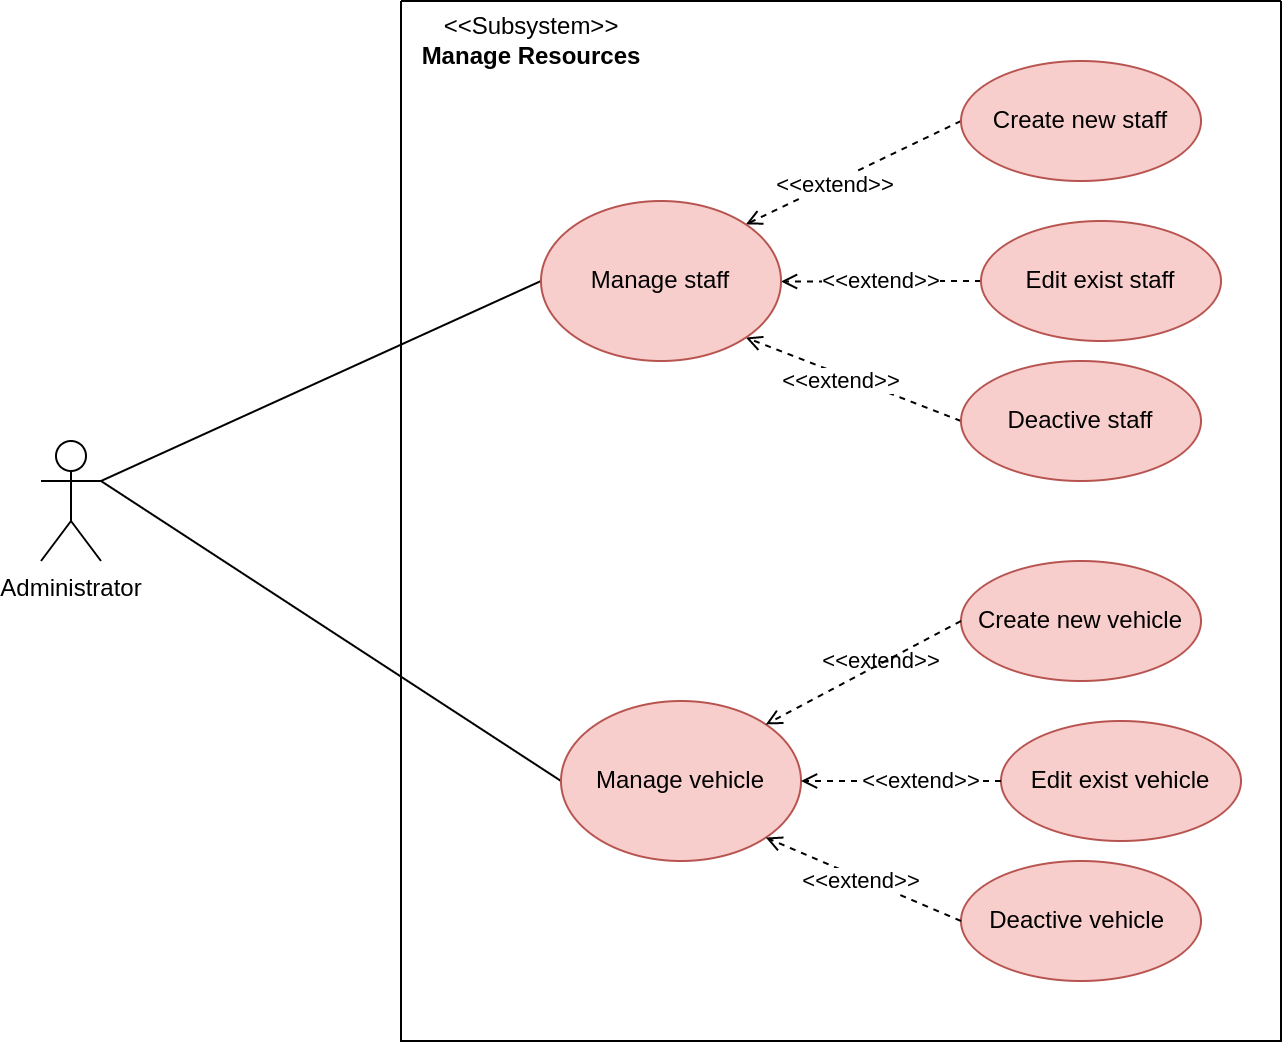
\includegraphics[width=0.70\linewidth]{imgs/use-case diagram/manageResources_uc.png}
        \caption{Use-case diagram chức năng kiểm soát tài nguyên}
    \end{figure}

    \vspace{1cm}
    \begin{tblr}{
        width=1\linewidth,
        hlines,
        vlines,
        colspec={X[3]X[7]},
        columns = {valign = m, },
        row{1} = {halign = c, valign = m, bg = lightgray, fg = black},
    }
        {\textbf{Use case name} & \textbf{Manage staff}}  \\
        Description	& Xếp lịch cho nhân viên \\
        Actor & 	Người quản lý (Administrator) \\
        Trigger & 	Người quản lý ấn vào phần quản lý nhân viên ở menu chính \\
        Pre-condition & Người quản lý đang ở quản lý tài nguyên \\
        Post-condition & Trang quản lý nhân viên được hiển thị \\
        Normal flow &   1. Hệ thống lấy dữ liệu về các nhân viên\newline
                    	2. Hệ thống hiện thị danh sách nhân viên lên màn hình \newline
                    	3. Người dùng chọn một nhân viên để thực hiện hành động \newline
                     	4. Hệ thống hiện thị thông tin chi tiết của nhân viên \\
        Extended points & 	Create new staff \newline
                        	Edit exist staff \newline
                        	Deactive staff \\
    \end{tblr}

    \begin{tblr}{
        width=1\linewidth,
        hlines,
        vlines,
        colspec={X[3]X[7]},
        columns = {valign = m, },
        row{1} = {halign = c, valign = m, bg = lightgray, fg = black},
    }
        {\textbf{Use case name} & \textbf{Create new staff}}  \\
        Description	& Tạo ra một nhân viên mới \\
        Actor & 	Người quản lý (Administrator) \\
        Trigger & 	Người quản lý ấn vào nút tạo người dùng mới \\
        Pre-condition & Người quản lý đang ở trong phần quản lý nhân viên \\
        Post-condition & Nhân viên mới được tạo ra \\
        Normal flow &   1. Hệ thống hiển thị các thông tin cần điền \newline
                    	2. Người dùng điền các thông tin \newline
                    	3. Hệ thống kiểm tra thông tin được điền \newline
                    	4. Người dùng ấn tạo nhân viên mới \newline
                    	5. Hệ thống ghi nhận nhân viên mới \newline
                    	6. Hệ thống thông báo tạo nhân viên thành công \\
        Alternative flow  & Alternative flow thứ 1: tại bước 1 \newline
                        	1a. Người dùng ấn nút hủy \newline
                        	1b. Quay lại màn hình thông tin chi tiết của nhân viên \\
        Exception flow & Exception flow thứ 1: tại bước 3 \newline
                    	 1a. Nếu thông tin sai, thông báo cho người dùng \newline
                    	 Quay lại bước 2  \\
    \end{tblr}

    \vspace{1cm}
    \begin{tblr}{
        width=1\linewidth,
        hlines,
        vlines,
        colspec={X[3]X[7]},
        columns = {valign = m, },
        row{1} = {halign = c, valign = m, bg = lightgray, fg = black},
    }
        {\textbf{Use case name} & \textbf{Edit exist staff}}  \\
        Description	& Chỉnh sửa một nhân viên  \\
        Actor & 	Người quản lý (Administrator) \\
        Trigger & 	Người quản lý ấn vào nút chỉnh sửa nhân viên \\
        Pre-condition & Người quản lý đang ở trong phần quản lý nhân viên \\
        Post-condition & Thông tin nhân viên được chỉnh sửa thành công\\
        Normal flow &   1. Hệ thống hiển thị các thông tin cần điền \newline
                    	2. Người dùng điền các thông tin \newline
                    	3. Hệ thống kiểm tra thông tin được điền \newline
                    	4. Người dùng ấn cập nhật nhân viên \newline
                    	5. Hệ thống ghi nhận thông tin được cập nhật \newline
                    	6. Hệ thống thông báo cập nhật nhân viên thành công \\
        Alternative flow  & Alternative flow thứ 1: tại bước 1 \newline
                        	1a. Người dùng ấn nút hủy \newline
                        	1b. Quay lại màn hình thông tin chi tiết của nhân viên \\
        Exception flow & Exception flow thứ 1: tại bước 3 \newline
                    	 1a. Nếu thông tin sai, thông báo cho người dùng \newline
                    	 Quay lại bước 2 \\
    \end{tblr}

    \begin{tblr}{
        width=1\linewidth,
        hlines,
        vlines,
        colspec={X[3]X[7]},
        columns = {valign = m, },
        row{1} = {halign = c, valign = m, bg = lightgray, fg = black},
    }
        {\textbf{Use case name} & \textbf{Deactive staff}}  \\
        Description	& Hủy kích hoạt một nhân viên \\
        Actor & 	Người quản lý (Administrator) \\
        Trigger & 	Người quản lý ấn vào nút hủy kích hoạt nhân viên \\
        Pre-condition & Người quản lý đang ở trong phần quản lý nhân viên \\
        Post-condition & Nhân viên bị hủy kích hoạt\\
        Normal flow &   1. Hệ thống hiểu thị xác nhận hủy kích hoạt nhân viên \newline
                    	2. Người dùng nhấn đồng ý \newline
                    	3. Hệ thống hủy kích hoạt nhân viên \newline
                    	4. Hệ thống thông báo hủy kích hoạt thành công \\
        Alternative flow  & Alternative flow thứ 1: tại bước 1 \newline
                        	1a. Người dùng ấn nút hủy \newline
                        	1b. Quay lại màn hình thông tin chi tiết của nhân viên \\
        Exception flow & none \\
    \end{tblr}

    \vspace{1cm}
    \quad Phần use-case senario của  Manage vehicle tương tự như trên.


	
\section{Activity diagram giữa hệ thống và các bên liên quan trong Task Assignment Module}
    \begin{figure}[h]
        \centering
        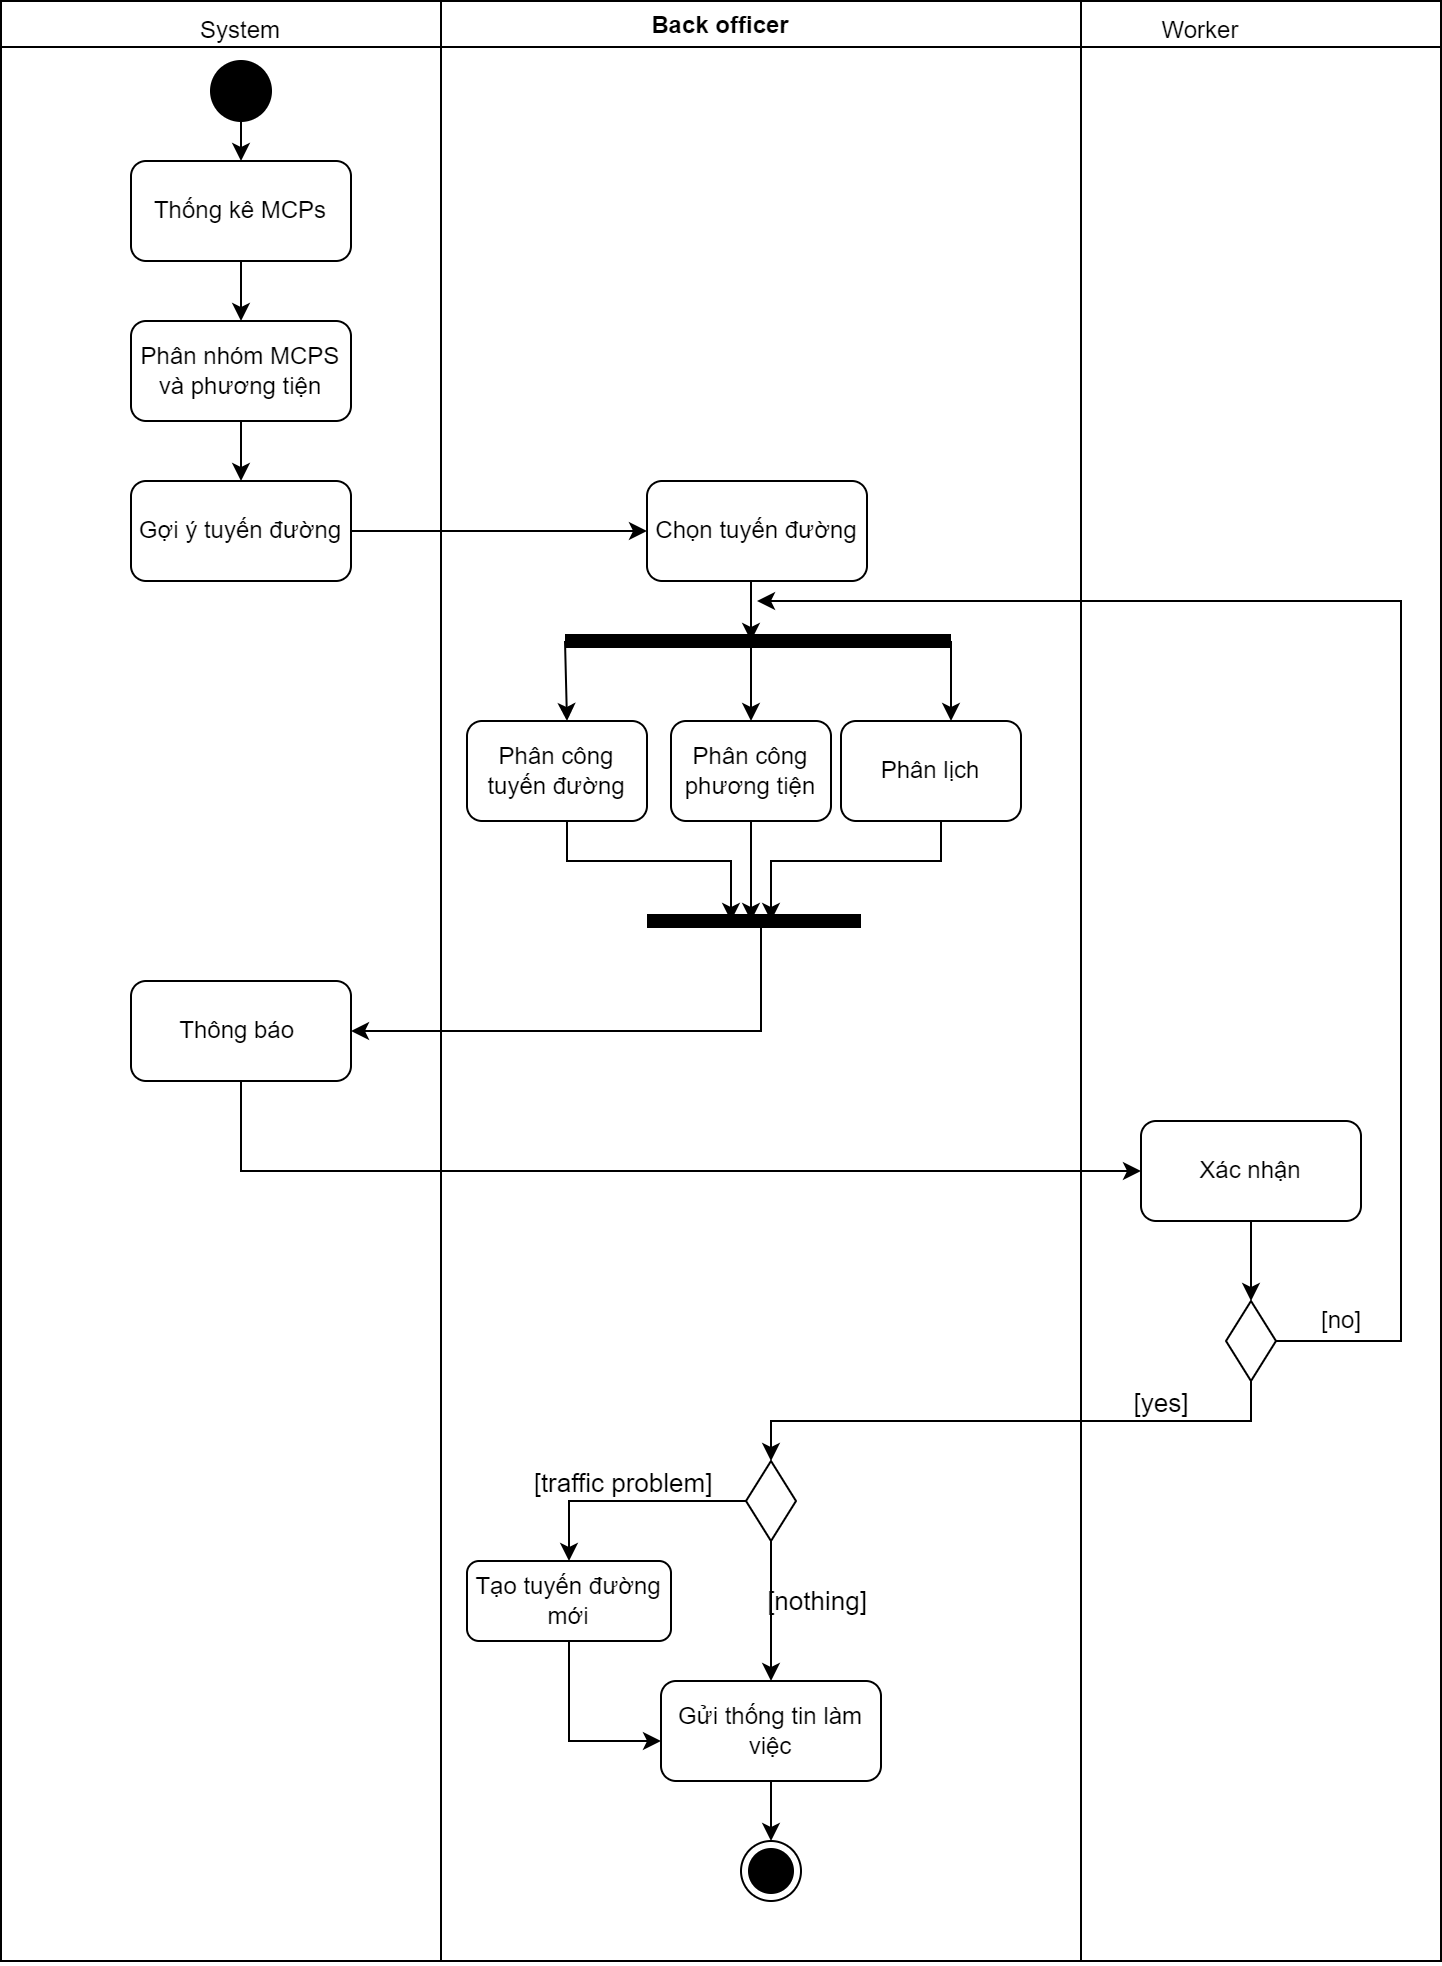
\includegraphics[width=15.0cm,height=15cm]{imgs/activity diagram/activity diagram.png}
        \caption{Activity diagram trong Task Asssignment Module}
    \end{figure}
    \newpage
    Hoạt động giữa hệ thống và các bên liên quan trong Task Assignment Module gồm các hoạt động theo thứ tự:
    \begin{enumerate}
        \item Bắt đầu.
        \item Hệ thống thống kê số lượng, vị trí MCPs.
        \item Hệ thống phân nhóm MCPs theo vùng phù hợp với sức chứa của phương tiện hiện có để tối ưu về tuyến đường và nhiên liệu.
        \item Hệ thống gợi ý các tuyến đường tối ưu cho Back officer.
        \item Back officer chọn tuyến đường cho tháng.
        \item Back officer phân công tuyến đường, phân phương tiện và tạo lịch cho collectors, janitors.
        \item Hệ thống gửi thông báo cho collectors, janitors.
        \item  Collectors, janitors xem thông báo được gửi.
        \item Back officer gửi thông tin làm việc theo ngày cho collectors, janitors.
        \item Kết thúc
    \end{enumerate}

\section{Giải pháp ý niệm cho task Route planning và Sequence diagram mô tả nó}
    \subsection{Giải pháp ý niệm cho task Route Planning}
        \textbf{Xét các Actor: }
    
        \begin{itemize}
            \item[-] Back Officer.
            \item[-] Cơ sở dữ liệu bản đồ (Map Database): một API cung cấp mọi thông tin về đường đi trong một vùng không gian nhất định khi được yêu cầu.
        \end{itemize}
    
        \textbf{Giả định:}
    
        \begin{itemize}
            \item[-] Back Officer đã đăng nhập thành công vào hệ thống.
            \item[-] Back Officer đã thao tác với hệ thống, đã nạp một danh sách các MCPs mà mình có nhu cầu tìm đường.
            \item[-] Map Database luôn hoạt động và hoạt động đúng kỳ vọng.
        \end{itemize}
    
        \textbf{Ta có, các entity liên quan:}
    
        \begin{itemize}
            \item[-] UIController: Hệ thống đảm nhiệm chức năng làm cầu nối, cho phép người dùng quản lý, sử dụng hệ thống.
            \item[-] RoutePlannerObject: Hệ thống đảm nhiệm chính chức năng tìm đường tự động và đánh giá đường đi.
        \end{itemize}
    
        \textbf{Các thao tác có thể thực hiện}
    
        \begin{itemize}
            \item[-] Back officer ra lệnh cho hệ thống tự tạo đường đi (route) phù hợp.
            \item[-] Back officer tự chỉnh sửa, thêm bớt các tuyến đường trong route mới hoặc route đã định sẵn từ thao tác trên.
        \end{itemize}
    
        \textbf{Mô tả chi tiết các thao tác}
        \begin{enumerate}
            \item Back officer ra lệnh cho hệ thống tự tạo đường đi (route) phù hợp.
            \begin{itemize}
                \item[-] Người dùng thực hiện lệnh tạo route tự động bằng cách ra lệnh GenerateRoute () lên hệ thống.
                \item[-] UIController nhận lệnh, thực hiện lệnh PlanRoute (MCPs, vehicles) lên hệ thống RoutePlannerObject với MCPs, vehicles là các MCP và phương tiện được dùng.
                \item[-] RoutePlannerObject thực hiện GetAvailablePaths (locations, vehicles) đối với Map Database để lấy đường đi hợp lệ giữa các vị trí của MCP mà phương tiện có thể di chuyển qua.
                \begin{itemize}
                    \item[+] Nếu tồn tại những đường đi hợp lệ, RoutePlannerObject tính toán route tốt nhất và trả về cho UIController. UIController trình thông tin về người dùng. Quá trình tự động tạo route kết thúc thành công.
                    \item[+] Nếu không tồn tại path nào, RoutePlannerObject trả về lỗi không tồn tại đường đi cho UIController. Quá trình tự động tạo route kết thúc không thành công.
                \end{itemize}
            \end{itemize}
        
            \item Back officer tự chỉnh sửa, thêm bớt các tuyến đường trong route mới hoặc route đã định sẵn từ thao tác trên.
            \begin{itemize}
                \item[-] UIController tự chờ mỗi khi người dùng chỉnh sửa, thêm/ bớt route trên giao diện, chạy lệnh ModifyRoute (route) với route là tổng hợp các route mới (mà người dùng đã thay đổi/ chỉnh sửa).
                \item[-] UIController tìm các path có trong route mới, qua lệnh ValidateRoute (paths, MCPs, vehicles) gửi paths vừa chỉnh sửa cho hệ thống RoutePlannerObject để đánh giá tính hợp lệ và hiệu quả.
                \item[-] RoutePlannerObject lấy những đường đi hợp lệ cho phương tiện giữa các MCP từ hệ cơ sở dữ liệu bản đồ bằng lệnh GetPathsBetween (locations, vehicles).
                \item[-] RoutePlannerObject đánh giá nếu đường đi trong route có hợp lệ so với các paths trên bản đồ.
                \begin{itemize}
                    \item[+] Nếu route là hợp lệ, trả về UIController độ hiệu quả của route. UIController trình thông tin đến người dùng và lưu route vào hệ thống. Quá trình chỉnh sửa/ thay đổi route thành công.
                    \item[+] Nếu route là không hợp lệ, trả về UIController sự hợp lệ của route. UIController trình thông tin đến người dùng, không lưu route mới vào hệ thống. Quá trình chỉnh sửa/ thay đổi route không thành công.
                \end{itemize}
            \end{itemize}
        \end{enumerate}
    \subsection{Sequence diagram mô tả giải pháp cho task Route Planning}
        \begin{figure}[H]
            \centering
            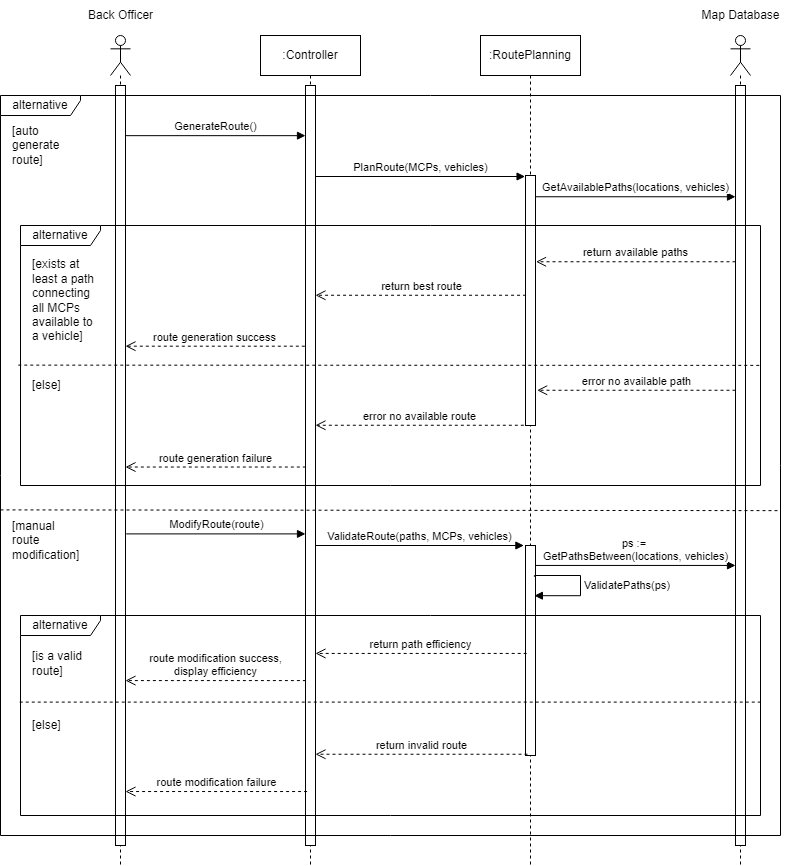
\includegraphics[width=1\linewidth]{imgs/sequence diagram/Sequence Diagram 2.2.png}
            \caption{Sequence diagram cho Task Route Planning}
        \end{figure}
    
        \newpage

\section{Class Diagram cho task assignment module}
     \begin{figure}[h]
        \centering
        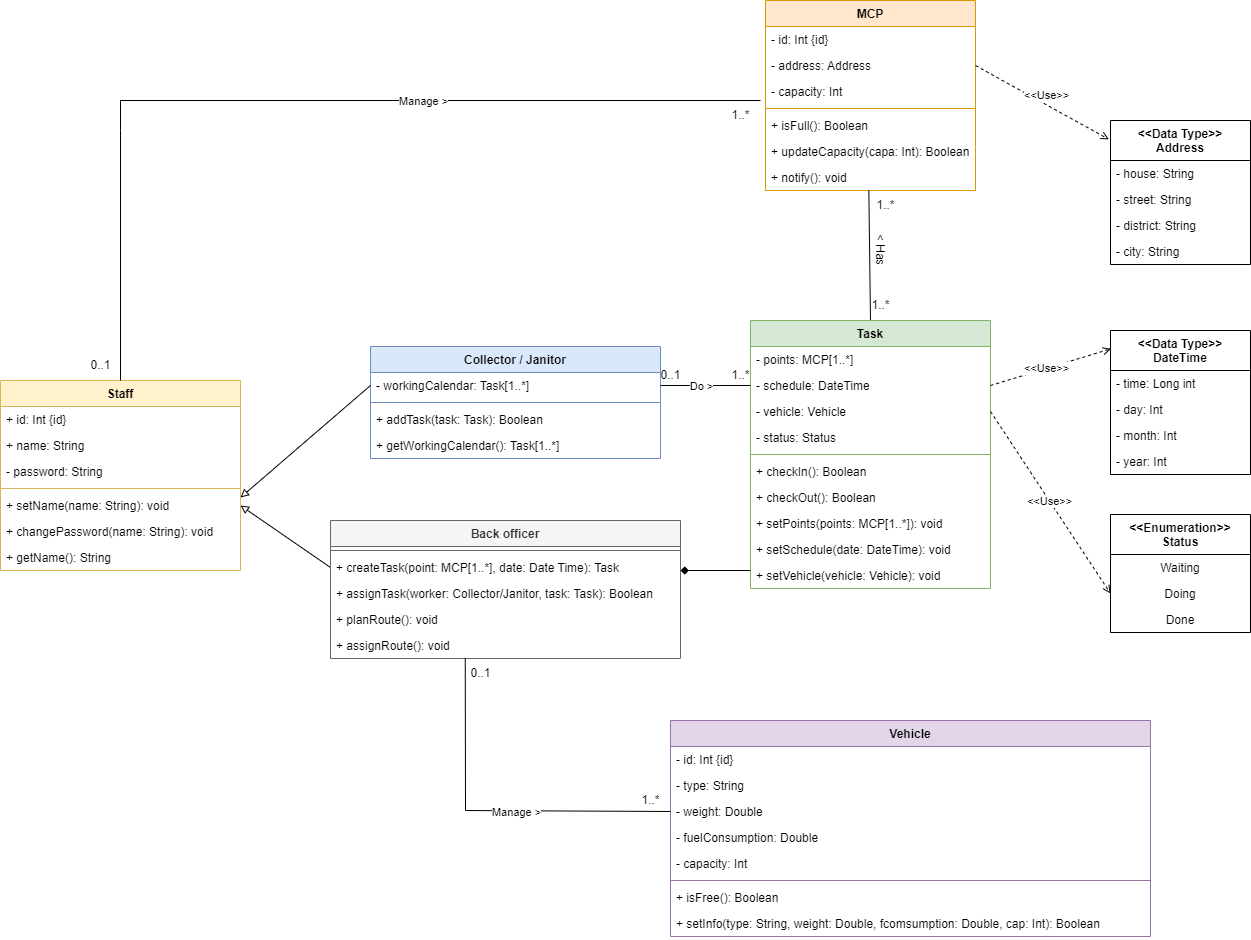
\includegraphics[width=15cm,height=15cm]{imgs/class diagram/class diagram.png}
        \caption{Class diagram cho task assignment module}
    \end{figure}

    \newpage
    -Có tất cả 6 class trong module trên gồm có:
    \begin{enumerate}
        \item Class Staff:
        \begin{table}[htp]
            \begin{tabular}{|lll|}
                \hline
                \multicolumn{1}{|l|}{Class Name} & \multicolumn{2}{l|}{Staff}                                     \\ \hline
                \multicolumn{1}{|l|}{Inherit}    & \multicolumn{2}{l|}{None}                                      \\ \hline
                \multicolumn{3}{|c|}{\cellcolor[HTML]{FFFFC7}Attributes}                                          \\ \hline
                \multicolumn{1}{|l|}{int}        & \multicolumn{1}{l|}{id}               & Số định danh nhân viên \\ \hline
                \multicolumn{1}{|l|}{string}     & \multicolumn{1}{l|}{name}             & Tên nhân viên          \\ \hline
                \multicolumn{1}{|l|}{string}     & \multicolumn{1}{l|}{password}         & Mật khẩu đăng nhập     \\ \hline
                \multicolumn{3}{|c|}{\cellcolor[HTML]{FFFFC7}Methods}                                             \\ \hline
                \multicolumn{1}{|l|}{void}       & \multicolumn{1}{l|}{setName()}        & Đặt tên cho nhân viên  \\ \hline
                \multicolumn{1}{|l|}{void}       & \multicolumn{1}{l|}{changePassword()} & Đổi mật khẩu           \\ \hline
                \multicolumn{1}{|l|}{string}     & \multicolumn{1}{l|}{getName()}        & Lấy tên nhân viên      \\ \hline
                \multicolumn{3}{|c|}{\cellcolor[HTML]{FFFFC7}Relationships}                                       \\ \hline
                \multicolumn{1}{|l|}{Manage}     & \multicolumn{2}{l|}{Quản lý thông tin các MCP}                 \\ \hline
            \end{tabular}
        \end{table}
                
        \item Class Collector / Janitor:
        \begin{table}[htp]
            \begin{tabular}{|lll|}
                \hline
                \multicolumn{1}{|l|}{Class Name} & \multicolumn{2}{l|}{Collector/Janitor}                              \\ \hline
                \multicolumn{1}{|l|}{Inherit}    & \multicolumn{2}{l|}{Staff}                                          \\ \hline
                \multicolumn{3}{|c|}{\cellcolor[HTML]{FFFFC7}Attributes}                                               \\ \hline
                \multicolumn{1}{|l|}{Task{[}{]}} & \multicolumn{1}{l|}{workingCalendar}      & Lịch làm việc           \\ \hline
                \multicolumn{3}{|c|}{\cellcolor[HTML]{FFFFC7}Methods}                                                  \\ \hline
                \multicolumn{1}{|l|}{boolean}    & \multicolumn{1}{l|}{addTask()}            & Thêm task vào phần lịch \\ \hline
                \multicolumn{1}{|l|}{Task{[}{]}} & \multicolumn{1}{l|}{getWorkingCalendar()} & Lấy, xem lịch làm việc  \\ \hline
                \multicolumn{3}{|c|}{\cellcolor[HTML]{FFFFC7}Relationships}                                            \\ \hline
                \multicolumn{1}{|l|}{Do}         & \multicolumn{2}{l|}{Collector và Janitor thực hiện task}            \\ \hline
            \end{tabular}
        \end{table}
            
        \item Class Back officer:
        \begin{table}[htp]
            \begin{tabular}{|lll|}
                \hline
                \multicolumn{1}{|l|}{Class Name}  & \multicolumn{2}{l|}{Back officer}                                     \\ \hline
                \multicolumn{1}{|l|}{Inherit}     & \multicolumn{2}{l|}{Staff}                                            \\ \hline
                \multicolumn{3}{|c|}{\cellcolor[HTML]{FFFFC7}Attributes}                                                  \\ \hline
                \multicolumn{3}{|c|}{\cellcolor[HTML]{FFFFC7}Methods}                                                     \\ \hline
                \multicolumn{1}{|l|}{Task}        & \multicolumn{1}{l|}{createTask()} & Tạo task                          \\ \hline
                \multicolumn{1}{|l|}{boolean}     & \multicolumn{1}{l|}{assignTask()} & Gán task cho collector và janitor \\ \hline
                \multicolumn{1}{|l|}{void}        & \multicolumn{1}{l|}{planRoute()}  & Tạo tuyến đường                   \\ \hline
                \multicolumn{3}{|c|}{\cellcolor[HTML]{FFFFC7}Relationships}                                               \\ \hline
                \multicolumn{1}{|l|}{Manage}      & \multicolumn{2}{l|}{Quản lý thông tin phương tiện}                    \\ \hline
                \multicolumn{1}{|l|}{Composition} & \multicolumn{2}{l|}{Bao gồm task}                                     \\ \hline
            \end{tabular}
        \end{table}
    
        \newpage
            
        \item Class Task:
        \begin{table}[htp]
            \begin{tabular}{|lll|}
                \hline
                \multicolumn{1}{|l|}{Class Name} & \multicolumn{2}{l|}{Task}                                          \\ \hline
                \multicolumn{1}{|l|}{Inherit}    & \multicolumn{2}{l|}{None}                                          \\ \hline
                \multicolumn{3}{|c|}{\cellcolor[HTML]{FFFFC7}Attributes}                                              \\ \hline
                \multicolumn{1}{|l|}{MCP{[}{]}}  & \multicolumn{1}{l|}{points}        & Danh sách các MCP của task    \\ \hline
                \multicolumn{1}{|l|}{DateTime}   & \multicolumn{1}{l|}{schedule}      & Thời gian làm cho task        \\ \hline
                \multicolumn{1}{|l|}{Vehicle}    & \multicolumn{1}{l|}{vehicle}       & Phương tiện dùng cho task     \\ \hline
                \multicolumn{1}{|l|}{Status}     & \multicolumn{1}{l|}{status}        & Trạng thái của task           \\ \hline
                \multicolumn{3}{|c|}{\cellcolor[HTML]{FFFFC7}Methods}                                                 \\ \hline
                \multicolumn{1}{|l|}{boolean}    & \multicolumn{1}{l|}{checkIn()}     & check in task                 \\ \hline
                \multicolumn{1}{|l|}{boolean}    & \multicolumn{1}{l|}{checkOut()}    & check out task                \\ \hline
                \multicolumn{1}{|l|}{void}       & \multicolumn{1}{l|}{setPoints()}   & Đặt danh sách MCP cho task    \\ \hline
                \multicolumn{1}{|l|}{void}       & \multicolumn{1}{l|}{setSchedule()} & Đặt lịch cho task             \\ \hline
                \multicolumn{1}{|l|}{void}       & \multicolumn{1}{l|}{setVehicle()}  & Đặt phương tiện dùng cho task \\ \hline
                \multicolumn{3}{|c|}{\cellcolor[HTML]{FFFFC7}Relationships}                                           \\ \hline
                \multicolumn{1}{|l|}{Has}        & \multicolumn{2}{l|}{Mang thông tin các MCP}                        \\ \hline
            \end{tabular}
        \end{table}
            
            
        \item Class Vehicle:
        \begin{table}[htp]
            \begin{tabular}{|lll|}
                \hline
                \multicolumn{1}{|l|}{Class Name} & \multicolumn{2}{l|}{Vehicle}                                                               \\ \hline
                \multicolumn{1}{|l|}{Inherit}    & \multicolumn{2}{l|}{None}                                                                  \\ \hline
                \multicolumn{3}{|c|}{\cellcolor[HTML]{FFFFC7}Attributes}                                                                      \\ \hline
                \multicolumn{1}{|l|}{int}        & \multicolumn{1}{l|}{id}              & Số định danh phương tiện                            \\ \hline
                \multicolumn{1}{|l|}{string}     & \multicolumn{1}{l|}{type}            & Loại phương tiện                                    \\ \hline
                \multicolumn{1}{|l|}{double}     & \multicolumn{1}{l|}{weight}          & Khối lượng phương tiện                              \\ \hline
                \multicolumn{1}{|l|}{double}     & \multicolumn{1}{l|}{fuelConsumption} & Mức tiêu thụ nhiên liệu                             \\ \hline
                \multicolumn{1}{|l|}{int}        & \multicolumn{1}{l|}{capacity}        & Sức chứa của phương tiện                            \\ \hline
                \multicolumn{3}{|c|}{\cellcolor[HTML]{FFFFC7}Methods}                                                                         \\ \hline
                \multicolumn{1}{|l|}{boolean}    & \multicolumn{1}{l|}{isFree()}        & Kiểm tra phương tiện có đang được sử dụng hay không \\ \hline
                \multicolumn{1}{|l|}{boolean}    & \multicolumn{1}{l|}{setInfo()}       & Đặt thông tin cho phương tiện                       \\ \hline
                \multicolumn{3}{|c|}{\cellcolor[HTML]{FFFFC7}Relationships}                                                                   \\ \hline
            \end{tabular}
        \end{table}
            
        \newpage
        \item Class MCP:
        \begin{table}[htp]
            \begin{tabular}{|lll|}
                \hline
                \multicolumn{1}{|l|}{Class Name} & \multicolumn{2}{l|}{MCP}                                                            \\ \hline
                \multicolumn{1}{|l|}{Inherit}    & \multicolumn{2}{l|}{None}                                                           \\ \hline
                \multicolumn{3}{|c|}{\cellcolor[HTML]{FFFFC7}Attributes}                                                               \\ \hline
                \multicolumn{1}{|l|}{int}        & \multicolumn{1}{l|}{id}               & Số định danh cho MCP                        \\ \hline
                \multicolumn{1}{|l|}{Address}    & \multicolumn{1}{l|}{address}          & Địa chỉ của MCP                             \\ \hline
                \multicolumn{1}{|l|}{int}        & \multicolumn{1}{l|}{capacity}         & Sức chứa của MCP                            \\ \hline
                \multicolumn{1}{|l|}{int}        & \multicolumn{1}{l|}{capacity}         & Sức chứa của phương tiện                    \\ \hline
                \multicolumn{3}{|c|}{\cellcolor[HTML]{FFFFC7}Methods}                                                                  \\ \hline
                \multicolumn{1}{|l|}{boolean}    & \multicolumn{1}{l|}{isFull()}         & Kiểm tra MCP có đang đầy chỗ chứa hay không \\ \hline
                \multicolumn{1}{|l|}{boolean}    & \multicolumn{1}{l|}{updateCapacity()} & Cập nhật lại sức chứa MCP                   \\ \hline
                \multicolumn{1}{|l|}{void}       & \multicolumn{1}{l|}{notify()}         & Thông báo khi MCP hết sức chứa              \\ \hline
                \multicolumn{3}{|c|}{\cellcolor[HTML]{FFFFC7}Relationships}                                                            \\ \hline
            \end{tabular}
        \end{table}
\end{enumerate}

	\section{Mô tả thiết kế kiến trúc để xây dựng hệ thống}
    \quad Sau khi xác định rõ bài toàn, dựa trên những yêu cầu cả về mặt chứng năng và phi chức năng, nhóm quyết định đưa ra thiết kế hệ thống như sau:

    \vspace{1cm}
    \begin{figure}[h]
    	\centering
    	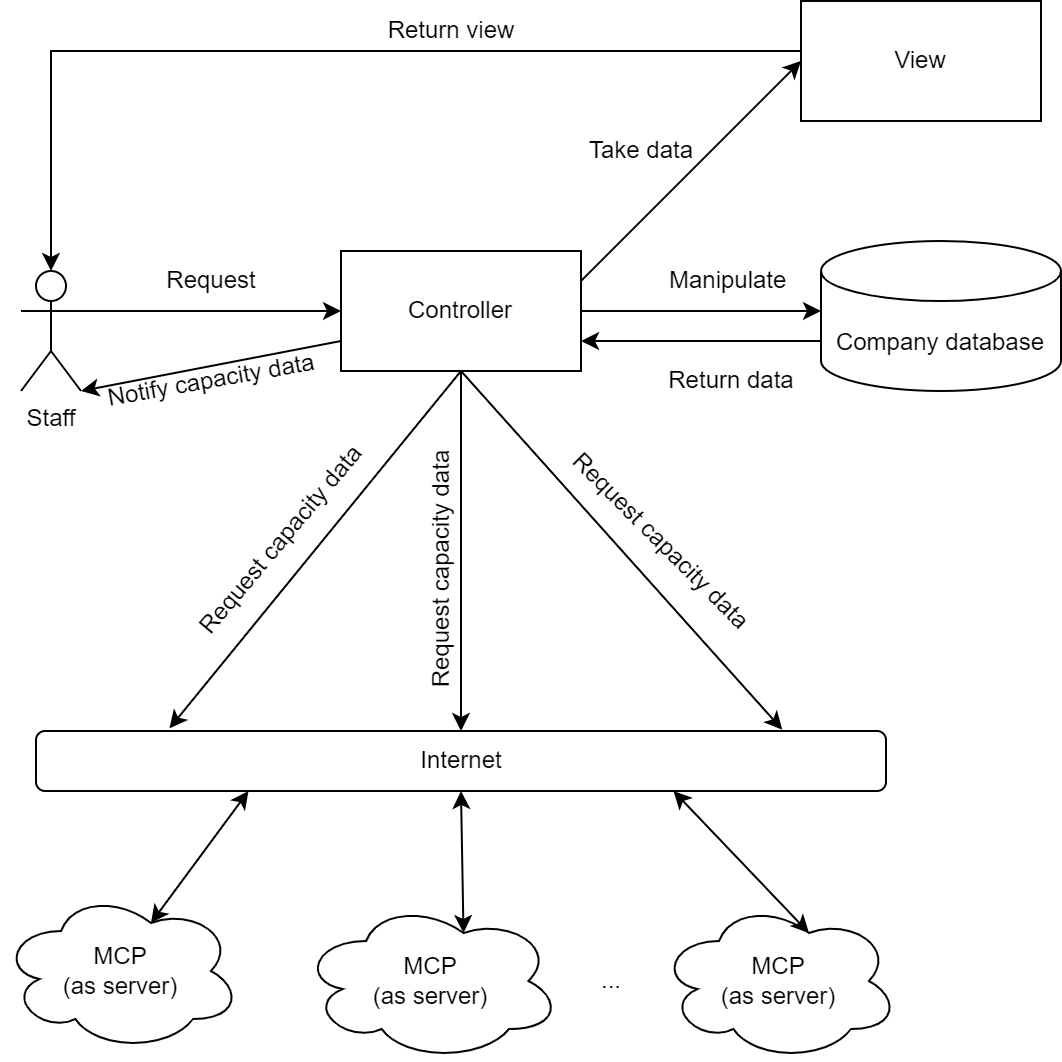
\includegraphics[width=1\linewidth]{imgs/architecture design.png}
    	\caption{Thiết kế kiến trúc của hệ thống}
    \end{figure}

   	\begin{tblr}{
   			width=1\linewidth,
   			hlines,
   			vlines,
   			colspec={X[3]X[7]},
   			columns = {valign = m, },
			column{1} = {halign = c},
   			row{1} = {halign = c, valign = m, bg = lightgray, fg = black},
   		}
   		{\textbf{Table} & \textbf{Architecture design}}  \\
   		Pattern		& 	MVC + Pub-sub \\
   		Description & 	1. Với các thông tin cơ bản như thông tin cá nhân, lịch làm, thông tin về phương tiện, ta sử dụng mô hình MVC để lấy dữ liệu và hiển thị lên cho người dùng. \newline
						\newline
		   				2. Với các thông tin về sức chứa của các MCP, ta sử dụng mô hình publisher - subscriber với Controller đóng vai trò là subscriber và MCP là các publisher. \newline
						\newline
		   				3. Với các thông báo về việc sức chứa của các MCP đạt mức tối đa ta sử dụng mô hình publisher - subscriber với Controller lúc này đóng vai trò là publisher và nhân viên là các subscriber. \\
		Flow & 			1. Controller nhận request từ người dùng -> gọi đến database thực hiện yêu cầu -> database gửi kết qua sau khi thực hiện lại cho controller -> controller gửi dữ liệu vừa nhận được cho phần View -> View hiển thị kết quả cho người dùng. \newline
						\newline
						2. Controller nhận dữ liệu từ tất cả các sensor của từng MCP sau mỗi 15 phút. Nếu sau ba lần controller không nhận được dữ liệu, sensor xem như bị mất kết nối và thực hiện thiết lập lại kết nối với sensor của MCP đó. \newline
						\newline
						3. Ngay sau khi nhận dữ liệu từ các sensor, controller thực hiện broadcast dữ liệu nếu sức chứa đã đầy đến collector/janitor liên quan đến MCP đó. \\
   	\end{tblr}

   	\vspace{0.5cm}

	\quad \textbf{Những nguyên nhân nhóm chọn kiến trúc trên:}
	\begin{enumerate}
		\item[-] MCP (Model - Controller - View) là kiểu kiến trúc bao gồm 3 chủ thể lớn là Controller - đảm nhiệm việc kiểm tra và thực hiện các yêu cầu được gửi đến, Model - đảm nhiệm việc truy suất dữ liệu của hệ thống và View - là cái được trả về cho người dùng, cái được hiển thị trên màn hình. MCP phù hợp với yêu cầu hiện thực ứng dụng trên nền tảng web, dễ dàng trong việc thiết kế, triển khai hệ thống.
		\item[-] Publisher - Subcriber cho cho phép hệ thống nhận thông tin liên tục về các điểm MCP và gửi đến người dùng những thông tin kịp thời nhất khi một hay nhiều điểm MCP bị đầy.
		\item[-] Xét tương đối với các kiến trúc khác:
		\begin{enumerate}
			\item[+] Mặc dù Layer và MCV đều được thiết kế theo kiểu module, trong đó các khối được tách ra đảm nhiệm từng chức năng riêng biệt, khi cần nâng cấp một module sẽ không ảnh hưởng đến hoạt động của các module khác. Tuy nhiên MVC có hiệu suất tốt hơn Layer, vì dữ liệu được truyền qua một tầng duy nhất, khác với việc khi truyền dữ liệu ở kiến trúc Layer phải đi qua nhiều lớp dẫn tới hao phí thời gian truyển dữ liệu từ lớp này sang lớp kia
			\item[+] Peer-to-Peer là kiểu thiết kế trong đó các client sẽ kết nối trực tiếp với nhau, trong trường hợp ứng dụng quản lý có số lượng lớn các client (bao gồm back officer, janitor, collect), việc kết nối trực tiếp các thiết bị sẽ gây ra sự chồng chéo, khó khăn trong việc kiểm soát cũng như bảo trì
			\item[+] Pipe-filter có lợi thế trong việc tách dữ liệu có độ phức tạp cao thành dữ liệu sạch thông qua các lớp màn lọc (filter), tuy nhiên hạn chế của kién trúc này là ở việc với những nguồn data khác nhau, nó sẽ yêu cầu một luồng riêng, khả năng tái sử dụng các luồng cũ rất thấp. Đối với bài toán mà nhóm đang giải quyết, việc dữ liệu mà các MCP trả về là khác nhau, nguyên nhân có thể do sự khác biệt về phần cứng hay phần mềm của các cảm biến, chính vì thế nếu sử dụng Pipe-filter thì ta phải tạo ra nhiều luồng xử lý đối với từng MCP.
		\end{enumerate}
	\end{enumerate}
  
	\newpage
   	\quad Đối với bài toán được đặt ra, ta sẽ có tổng cộng 6 module. Bao gồm:
   	\begin{enumerate}
   		\item Module Xác thực

   		\begin{tblr}{
   				width=1\linewidth,
   				hlines,
   				vlines,
   				colspec={X[3]X[7]},
   				columns = {valign = m, },
   			}
   			Input & Người dùng X \\
   			Output & Người dùng X có được truy cập hay không \newline
   					 Vai trò của người dùng X là gì \\
   			Method & Validation() \newline
   			 		 Login() \newline
   			 		 Logout() \newline
   			 		 ChangePassword() \\
   		\end{tblr}

   		\item Module Chat

  		\begin{tblr}{
  				width=1\linewidth,
  				hlines,
  				vlines,
  				colspec={X[3]X[7]},
  				columns = {valign = m, },
  			}
  			Input & Tin nhắn, văn bản\\
  			Output & Hệ thống gửi tin nhắn cho người dùng \newline
  					 Người dùng nhận được tin nhắn \\
  			Method & ConnectUser() \newline
		  			 SendMessage() \newline
		  			 NotifyMessage() \\
  		\end{tblr}

  		\item Module View information

  		\begin{tblr}{
  				width=1\linewidth,
  				hlines,
  				vlines,
  				colspec={X[3]X[7]},
  				columns = {valign = m, },
  			}
  			Input & MCP X \newline
  			Phương tiện Y \newline
  			Nhân viên Z \\
  			Output & Thông tin của MCP X \newline
  			Thông tin phương tiện Y \newline
  			Thông tin nhân viên và lịch làm của nhân viên Z \\
  			Method & ShowInfoMCP() \newline
  			ShowInfoVehicle() \newline
  			ShowInfoStaff() \newline
  			ShowDailyTask() \newline
  			ShowCalendar() \\
  		\end{tblr}
   		

   		\item Module Manage Resource

   		\begin{tblr}{
   				width=1\linewidth,
   				hlines,
   				vlines,
   				colspec={X[3]X[7]},
   				columns = {valign = m, },
   			}
   			Input & Nhân viên X, phương tiện Y\\
   			Output & Nhân viên X được chỉnh sửa \newline
   					 Phương tiện Y được chỉnh sửa \\
   			Method & AddUser() \newline
		   		     EditUser() \newline
		   			 DeactivateUser() \newline
   					 \newline
		   			 AddVehicle() \newline
		   			 EditVehicle() \newline
		   			 DeactivateVehicle() \\
   		\end{tblr}
   		
		\newpage
   		\item Module Planning route

   		\begin{tblr}{
   				width=1\linewidth,
   				hlines,
   				vlines,
   				colspec={X[3]X[7]},
   				columns = {valign = m, },
   			}
   			Input & MCP, Vehicle \\
   			Output & Tuyến đường khả dụng \\
   			Method & GenerateRoute() \newline
	   				 PlanRoute() \newline
	   				 GetAvailablePaths() \newline
	   				 ModifyRoute() \newline
	   				 ValidateRoute() \newline
	   				 GetPathsBetween() \newline
	   				 ValidatePath() \\
   		\end{tblr}

   		\item Module Task assign

   		\begin{tblr}{
   				width=1\linewidth,
   				hlines,
   				vlines,
   				colspec={X[3]X[7]},
   				columns = {valign = m, },
   			}
   			Input &	Nhân viên X \newline
   				    Công việc Y \\
   			Output & Công việc được chia thành công cho nhân viên \newline
   					 Thông báo lịch làm cho nhân viên \\
   			Method & CreateTask() \newline
   					 SetMCP() \newline
   					 SetVehicle() \newline
   					 SetSchedule() \newline
   					 AssignTask() \\
   		\end{tblr}

   	\end{enumerate}
\newpage

\section{Component Diagram cho Task Assignment Module}
    \subsection{Component Diagram Task Assignment}
         \begin{figure}[h]
            \centering
            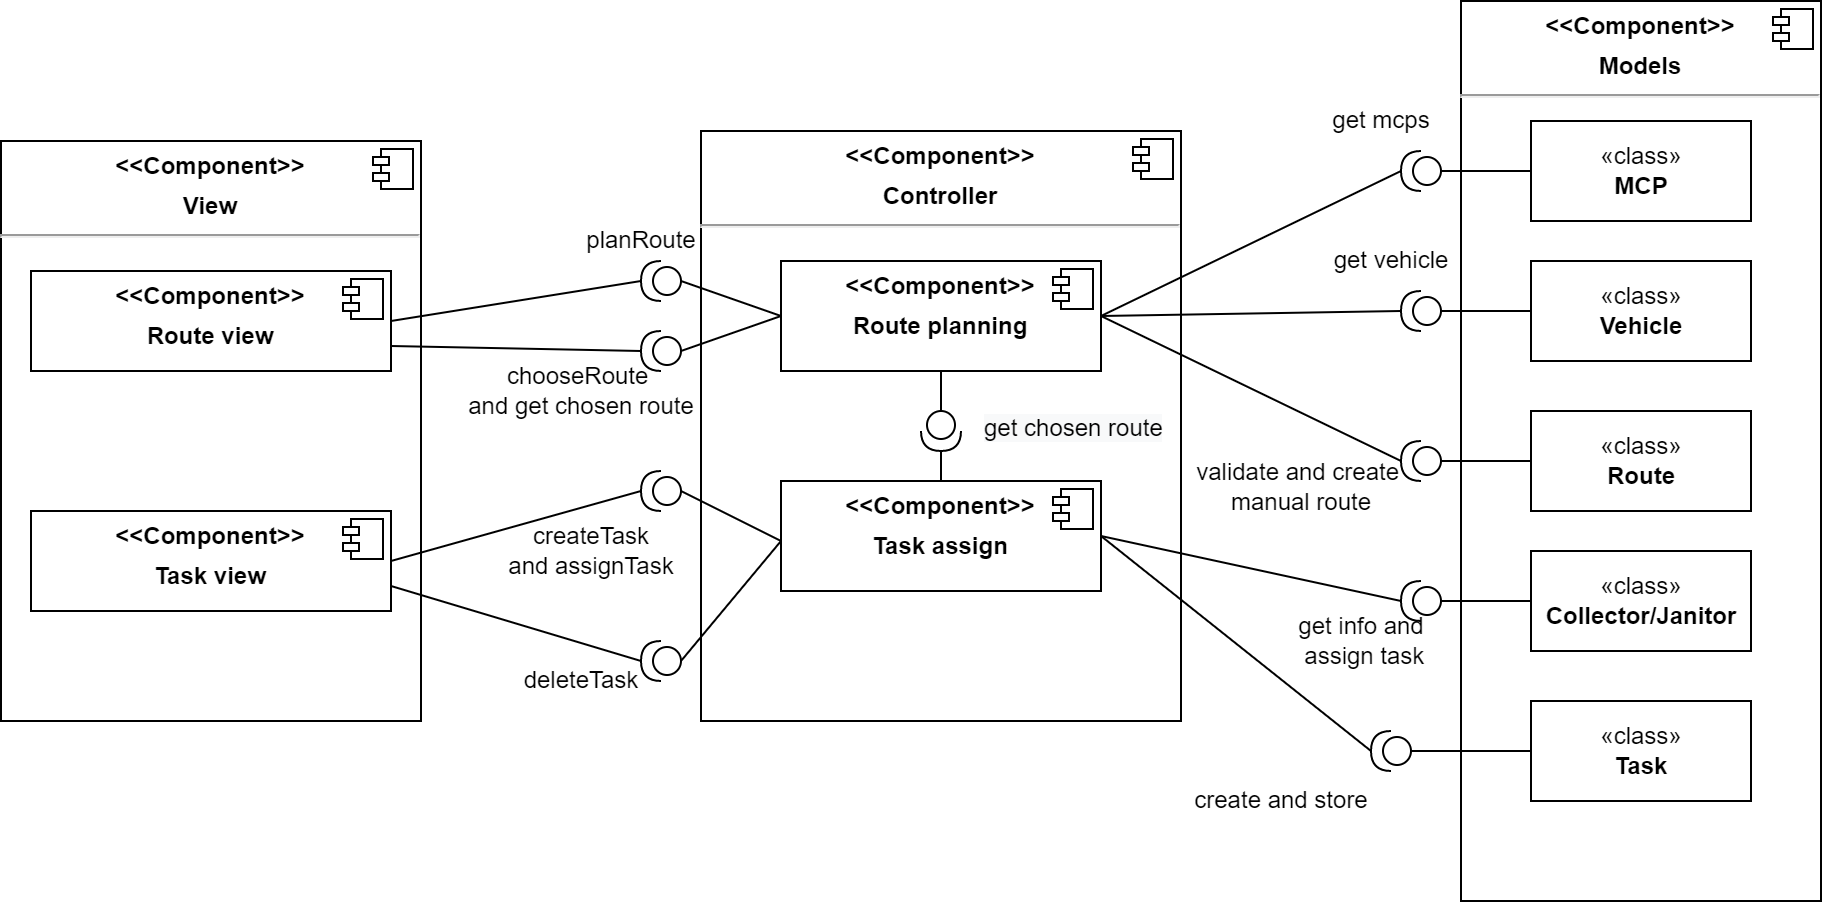
\includegraphics[width=1\linewidth]{imgs/component diagram/component Task Assignment.png}
            \caption{Component diagram cho task assignment module}
        \end{figure}
        Component diagram Task Asignment module gồm 5 Component với luồng thực thi:
        \begin{enumerate}
            \item Đưa dữ liệu Vehicle và MCPs vào Component Planning route và trả về tuyến đường khả dụng.
            \item Đưa dữ liệu các tuyến đường khả dụng vào component Choose route và trả về tuyến đường đã được Back Officer chọn.
            \item Đưa tuyến đường được chọn và Task vào Component Assign route, dữ liệu trả về là Task đã được Assign route.
            \item Đưa dữ liệu Task đã được Assign vào component Schedule time và trả về dữ liệu là Task được định thời gian thực hiện.
            \item Đưa lịch làm đã xếp và Worker vào component Assign staff và trả về kết quả là Task đã được Assign Worker, vehicle, route, calendar.
        \end{enumerate}
    \subsection{Component Diagram cho Planning Route }
        \begin{figure}[h]
            \centering
            \includegraphics[width=1\linewidth]{imgs/Component diagram/Component planning route.png}
            \caption{Component diagram cho Planning Route}
        \end{figure}
        Component diagram cho Planning Route gồm 2 Component thừa kế Component Modification Method với luồn thực thi:
        \begin{itemize}
            \item Auto generate route:
            \begin{enumerate}
                \item Đưa dữ liệu Vehicle, MCPs vào Component Get Avaiable Paths và trả về tuyến đường khả thi.
                \item Đưa dữ liệu các tuyến đường khả dụng vào Component Generate routes and Efficiency Statistic và trả về kết quả là tuyến đường hiệu quả để sử dụng.
            \end{enumerate}

            \item Manual generate route:
            \begin{enumerate}
                \item Đưa dữ liệu tuyến đường vào Component Validate Routes để kiểm thử và trả về tuyến đường đã được kiểm tra.
                \item Đưa tuyến đường đã được kiểm tra vào Component Generate routes and Efficiency Statistic và trả về kết quả là tuyến đường hiệu quả để sử dụng.
            \end{enumerate}
        \end{itemize}
       
       


\end{document}


\documentclass[a4paper]{article}
\usepackage{amssymb,epsfig,latexsym,multicol,array,hhline,fancyhdr}
\usepackage{vntex}
\usepackage{xcolor}
\usepackage{titlesec}
\usepackage{mdframed}
\usepackage{amsmath}
\usepackage{lastpage}
\usepackage[lined,boxed,commentsnumbered]{algorithm2e}
\usepackage{enumerate}
\usepackage{color}
\usepackage[most]{tcolorbox}
\usepackage{graphicx}
\usepackage{array}
\usepackage{float}
\usepackage{tabularx, caption}
\usepackage{tabularray}
\usepackage{colortbl}
\usepackage{longtable}
\usepackage{multirow} 
\usepackage{multicol}
\usepackage{rotating}
\usepackage{graphics}
\usepackage{geometry}
\usepackage{setspace}
\usepackage{epsfig}
\usepackage{wrapfig}
\usepackage{tikz}
\usepackage[most]{tcolorbox}
\usepackage{hyperref}
\usepackage{cleveref}
\usepackage{setspace}
\usepackage{subfiles}
\usepackage{indentfirst}

\hypersetup{urlcolor=blue,linkcolor=black,citecolor=black,colorlinks=true} 
\usetikzlibrary{arrows,snakes,backgrounds}

\newtheorem{theorem}{{\bf Theorem}}
\newtheorem{property}{{\bf Property}}
\newtheorem{proposition}{{\bf Proposition}}
\newtheorem{corollary}[proposition]{{\bf Corollary}}
\newtheorem{lemma}[proposition]{{\bf Lemma}}

\AtBeginDocument{\renewcommand*\contentsname{Nội dung}}
\AtBeginDocument{\renewcommand*\refname{Tham khảo}}
\setlength{\headheight}{40pt}
\pagestyle{fancy}

\fancyhead{}
\fancyhead[L]{
 \begin{tabular}{rl}
    \begin{picture}(25,15)(0,0)
    \put(0,-8){
\includegraphics[width=8mm, height=8mm]{imgs/hcmut.png}}
    %\put(0,-8){\epsfig{width=10mm,figure=hcmut.eps}}
   \end{picture}&
	%
\includegraphics[width=8mm, height=8mm]{hcmut.png} & %
	\begin{tabular}{l}
		\textbf{\bf \ttfamily Đại học Bách Khoa Thành phố Hồ Chí Minh}\\
		\textbf{\bf \ttfamily Khoa Khoa học và Kỹ thuật Máy tính}
	\end{tabular} 	
 \end{tabular}
}
\fancyhead[R]{
	\begin{tabular}{l}
		\tiny \bf \\
		\tiny \bf 
	\end{tabular} 
}
\fancyfoot{} 
\fancyfoot[L]{\scriptsize \ttfamily Bài tập lớn môn Công nghệ phần mềm - Năm học 2022-2023}
\fancyfoot[R]{\scriptsize \ttfamily Trang {\thepage}/\pageref{LastPage}}

\renewcommand{\headrulewidth}{0.3pt}
\renewcommand{\footrulewidth}{0.3pt}


%%%
\setcounter{secnumdepth}{4}
\setcounter{tocdepth}{3}
\makeatletter
\newcounter {subsubsubsection}[subsubsection]
\renewcommand\thesubsubsubsection{\thesubsubsection .\@alph\c@subsubsubsection}
\newcommand\subsubsubsection{\@startsection{subsubsubsection}{4}{\z@}%
                                     {-3.25ex\@plus -1ex \@minus -.2ex}%
                                     {1.5ex \@plus .2ex}%
                                     {\normalfont\normalsize\bfseries}}
\newcommand*\l@subsubsubsection{\@dottedtocline{3}{10.0em}{4.1em}}
\newcommand*{\subsubsubsectionmark}[1]{}
\makeatother


\begin{document}

	\begin{titlepage}
    \begin{center}
        ĐẠI HỌC QUỐC GIA THÀNH PHỐ HỒ CHÍ MINH\\
        TRƯỜNG ĐẠI HỌC BÁCH KHOA \\
        KHOA KHOA HỌC VÀ KỸ THUẬT MÁY TÍNH
    \end{center}

    \vspace{0.4cm}

    \begin{figure}[h!]
        \begin{center}
        
\includegraphics[width=4.5cm]{imgs/hcmut.png}
        \end{center}
    \end{figure}

    \vspace{0.1cm}


    \begin{center}
        \begin{tabular}{c}
        \textbf{{ \Large CÔNG NGHỆ PHẦN MỀM (CO3001)}}\\
        ~~\\
        \hline
        \\
        \multicolumn{1}{l}{\textbf{{\Large Bài tập lớn}}}\\
        \\
        \textbf{\Huge \color{red} URBAN WASTE COLLECTION}\\\\
        \textbf{\Huge \color{red} AID - UWC 2.0}\\
        \\
        \hline
        \end{tabular}
    \end{center}

    \vspace{0.5cm}

    \begin{table}[h]
        \begin{tabular}{rrl}
            \hspace{5 cm} & GVHD: & Lê Đình Thuận.\\
            & Lớp: & L04\_ Nhóm: Tình Đồng Chí \\
            & Sinh viên thực hiện: & Lê Nguyễn Huyền Thoại – 2012122.\\
            & & Trương Huy Thái – 2012036.\\
            & & Nguyễn Tiến Nam – 2011652.\\
            & & Nguyễn Trọng Đức Huy – 2011283.\\
            & & Nguyễn Trọng Nhân – 2011744.\\
            & & Trần Tuấn Anh – 2010878.\\
            & & Phan Thị Quỳnh Như – 2011780. \\
        \end{tabular}
    \end{table}

    \vspace{0.3CM}

    \begin{center}
        {\footnotesize THÀNH PHỐ HỒ CHÍ MINH, THÁNG \the\month /\the\year}
    \end{center}
\end{titlepage}


	\newpage
	\tableofcontents

	\newpage
	\section{Danh sách thành viên \& Khối lượng công việc}

\begin{tblr}{
    width=1\linewidth,
    hlines,
    vlines,
    colspec={X[-2]X[4]X[1.5]X[6]X[-1]},
    columns = {valign = m, },
    column{1} = {halign = c, },
    row{1} = {halign = c, valign = m, bg = lightgray, fg = black},
}
    {\textbf{STT} & \textbf{Họ và tên} & \textbf{MSSV} & \textbf{Công việc} & \textbf{Hoàn thành} }  \\
    1 & Lê Nguyễn Huyền Thoại & 2012122 & - Quản lý tiến độ công việc \newline
                                          - Thiểt kế use-case diagram tổng \newline
                                          - Thiệt kế class diagram \newline
                                          - Thiết kế component diagram
                                        & 100\% \\
    2 & Trương Huy Thái       & 2012036 & - Xác định yêu cầu phi chức năng \newline
                                          - Thiết kế use-case diagram task assignment \newline
                                          - Thiết kế activity diagram  \newline
                                          - Thiết kế architecture design
                                        & 100\% \\
    3 & Nguyễn Tiến Nam		  & 2011652 & - Xác định yêu cầu chức năng \newline
                                          - Viết đặc tả use-case tổng \newline
                                          - Thiết kế class diagram \newline
                                          - Thiết kế architecture design
                                        & 100\% \\
    4 & Nguyễn Trọng Đức Huy  & 2011283 & - Xác định ngữ cảnh dự án \newline
                                          - Thiết kế use-case manage resources \newline
                                          - Thiết kế sequence diagram \newline
                                          - Đánh giá Architecture design
                                        & 100\% \\
    5 & Nguyễn Trọng Nhân     & 2011744 & - Xác định ngữ cảnh dự án \newline
                                          - Viết đặc tả use-case task assignment \newline
                                          - Thiết kế sequence diagram \newline
                                          - Thiết kế component diagram
                                        & 100\% \\
    6 & Trần Tuấn Anh         & 2010878 & - Xác định yêu cầu phi chức năng \newline
                                          - Đánh giá các use-case diagram \newline
                                          - Thiết kế activity diagram \newline
                                          - Đánh giá component diagram
                                        & 100\% \\
    7 & Phan Thị Quỳnh Như    & 2011780 & - Xác định yêu cầu chức năng \newline
                                          - Đánh giá activity diagram, sequence diagram, class diagram \newline
                                          - Đánh giá tổng quan task 3 \newline
                                          - Viết báo cáo
                                        & 100\% \\

\end{tblr}


	%%%%%%%%%%%%%%%%%%%%%%%%%%%%%%%%%


	%%%%%%%%%%%%%%%%%%%%%%%%%%%%%%%%%
	\newpage
	\subsection{Mô tả chung}
    \quad Sau đại dịch covid-19, sức khỏe đã và đang là một trong những vấn đề được nhiều người quan tâm. Nhận thấy được vấn đề này, nhóm muốn tạo ra một ứng dụng nhằm nâng cao sức khỏe của người sử dụng bằng việc đưa ra những món ăn phù hợp với mục tiêu nhu cầu của từng người. Ví dụ như người dùng muốn tăng cân, tăng cơ, phần mềm sẽ đưa ra các món ăn làm sao để trong một khoảng thời gian nhất định, người dùng có thể đạt được cân nặng mà họ mong muốn. Ngoài ra nó còn cung cấp cho người dùng một lượng lớn các công thức nấu ăn đơn giản mà vẫn ngon miệng, phù hợp với cuộc sống ngày càng nhanh hiện nay.\\
    
    \begin{figure}[h]
        \centering
        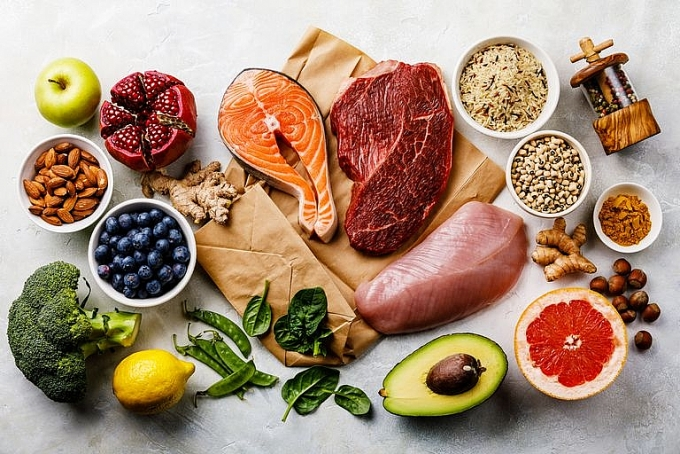
\includegraphics[width=0.7\linewidth]{images/healthy-food.jpg}
        \caption{Các chất có trong bữa ăn}
    \end{figure}
\section{Xác định ngữ cảnh của dự án UWC 2.0}
    \subsection{Các bên liên quan (Relevant Stakeholders)}
        \begin{enumerate}
            \item Công ty cung cấp dịch vụ thu dọn rác Y, ở vai trò là người quản lý.
            \item Công ty cung cấp dịch vụ thu dọn rác Y, ở vị trí là người sở hữu phần mềm UWC 2.0.
            \item Tổ chức X, phát triển phần mềm UWC 2.0.
            \item Công nhân sử dụng phần mềm UWC 2.0.
            \item Các bên liên quan khác (chính phủ, người dân).
        \end{enumerate}
    
    \subsection{Những mong muốn của các bên liên quan}
        \begin{enumerate}
            \item Công ty cung cấp dịch vụ thu dọn rác Y, ở vai trò là người quản lý, họ mong muốn phần mềm UWC 2.0 sẽ mang lại cho công ty:
            \begin{itemize}
                \item[-] Khả năng quản lý nhân lực, kiểm tra một cách hiệu quả cũng như thường xuyên cập nhật thông tin về sức chứa của các điểm tập trung rác thải (MCPs) và những thông tin nhằm phục vụ nhu cầu bảo trì các phương tiện vận chuyển, trang thiết bị của công ty.
                \item[-] Nâng cao hiệu suất thu gom rác thải của công ty.
                \item[-] Hệ thống khi được đưa vào hoạt động có độ tin cậy cao, hoạt động tốt trong mọi tình huống.
            \end{itemize}
            
            \item Công ty cung cấp dịch vụ thu dọn rác Y, ở vị trí là người sở hữu phần mềm UWC 2.0, họ sẽ có những mong muốn:
            \begin{itemize}
                \item[-] Khả năng mở rộng phạm vi hoạt động của hệ thống, không chỉ là trong một vùng, một quận cố định, mà có thể xử lý trong phạm vi toàn thành phố.
                \item[-] Chi phí và lợi nhuận luôn là một trong những vấn đề ưu tiên hàng đầu cần phải được cân nhắc. Khi được đưa vào sử dụng, UWC 2.0 phải đảm bảo tối ưu hóa về mặt nhiên liệu để từ đó giảm thiểu được chi phí phải bỏ ra. Thêm vào đó là chi phí để bảo trì hệ thống cũng phải phù hợp với công ty.
                \item[-] Trước đây công ty đã có sẵn hệ thống UWC 1.0 và công ty mong muốn có thể tận dụng lại tối đa dữ liệu có sẵn từ phiên bản trước và khả năng tương thích ngược giữa phiên bản 1.0 và 2.0.
                \item[-] Đem lại những kết quả tích cực đến công tác xử lý và tái chế rác thải trong cộng đồng, tạo ra môi trường sống xanh, sạch, đẹp cho người dân.
            \end{itemize}
      
            \item Tổ chức X, phát triển phần mềm UWC 2.0 có mong muốn:
            \begin{itemize}
                \item[-] Xây dựng được hệ thống có thể làm được và làm tốt những yêu cầu tối thiểu được yêu cầu bởi công ty chủ quản, xa hơn nữa là hoàn thiện hệ thống một cách tối ưu.
                \item[-] Hệ thống khi đến tay khách hàng phải dễ dàng bảo dưỡng, để nếu trong tương lai nếu khách hàng có thuê một công ty khác sửa chữa, bảo dưỡng hệ thống cũng thuận tiện hơn.
            \end{itemize}
        
            \item Công nhân sử dụng phần mềm UWC 2.0 mong muốn:
            \begin{itemize}
                \item[-] Vì đa phần người dùng là các cô chú trung niên, lớn tuổi, phần mềm nên có giao diện thân thiện, dễ dàng tiếp cận và làm quen.
                \item[-] Có thể sử dụng phần mềm trên nhiều thiết bị khác nhau như máy tính, điện thoại hay máy tính bảng.
                \item[-] Phần mềm phải sử dụng ổn định, ít giật lag và độ tin cậy cao.
            \end{itemize}
       
            \item Các bên liên quan khác (chính phủ, người dân): mong muốn phần mềm sẽ mang lại những ảnh hưởng tích cực đến công tác quản lý và tái sử dụng rác thải trong phạm vi khu vực và trong cả nước.
        \end{enumerate}
    
    \subsection{Vấn đề các bên liên quan đang gặp phải}
        \begin{enumerate}
            \item Công ty cung cấp dịch vụ thu dọn rác Y hiện đang gặp phải các vấn đề:
            \begin{itemize}
                \item[-] Công ty đang thiếu khả năng kiểm tra tình trạng trang thiết bị và phương tiện nên việc hoạt động chưa hiệu quả.
                \\
                \emph{\underline{Ví dụ}}: Chưa kiểm soát được tải trọng, sức chứa, tiêu thụ nhiên liệu dẫn tới sự phân bố xe chưa hợp lý khi hoạt động.
                
                \item[-] Việc quản lý nhân lực của công ty chưa hiệu quả:
                \begin{itemize}
                    \item[+] Công ty chưa theo dõi được tiến độ làm việc, hiệu suất làm việc của nhân viên.
                    \item[+] Việc phân công công việc chưa hợp lý gây mất công bằng và giảm hiệu suất công việc.
                \end{itemize}
            \end{itemize}
            
            \item Công ty cung cấp dịch vụ thu dọn rác Y, ở vị trí là người sở hữu hệ thống đang gặp phải các vấn đề:
            \begin{itemize}
                \item[-] Khả năng duy trì và nâng cấp hệ thống. Việc duy trì hệ thống đang có chi phí cao, chưa hợp lý.
                \item[-] Khi gặp các sự cố bất ngờ như  tai nạn, hư hỏng thiết bị thì việc liên lạc để điều phối nhân viên chưa kịp thời .
                \item[-] Công ty gặp bất tiện trong việc theo dõi và phân công lịch trình: lịch trình giấy, phân công thủ công. Điều này khiến công ty mất nhiều thời gian, nhân sự và việc phân công này chưa được tối ưu.
            \end{itemize}
            
            \item Các bên liên quan khác (chính phủ, người dân): Việc cải thiện môi trường chưa được tối ưu hoá, chi phí cao nhưng chưa hiệu quả dẫn đến lãng phí.
        \end{enumerate}
    
    \subsection{Lợi ích mà các bên liên quan có thể đạt được khi sử dụng hệ thống UWC 2.0}
        \begin{enumerate}
            \item Nhà cung cấp dịch vụ thu dọn rác Y ở vai trò quản lý:
            \begin{itemize}
                \item[-] Nắm bắt được cụ thể tình trạng hiện tại của các trang thiết bị và cơ sở vật chất, từ đó có thể đưa ra được những quyết định như nâng cấp, sửa chữa hay bổ sung trang thiết bị cho công nhân một cách kịp thời và hiệu quả.
                \item[-] Nhanh chóng theo dõi được tiến độ, hiệu suất làm việc của nhân viên. Đưa ra được phương án giải quyết sự cố kịp thời và công bằng.
            \end{itemize}
    
            \item Nhà cung cấp dịch vụ Y dưới góc độ chủ sở hữu hệ thống:
            \begin{itemize}
                \item[-] Tiết kiệm được chi phí duy trì và phát triển hệ thống.
                \item[-] Mang lại danh tiếng cho công ty trong mảng thu dọn rác thải.
            \end{itemize}
    
            \item Tổ chức X qua vai trò nhà phát triển phần mềm:
            \begin{itemize}
                \item[-] Tăng thu nhập cho công ty cũng như thu nhập của các cá nhân tham gia phát triển hệ thống.
                \item[-] Tăng kỹ năng của từng cá nhân.
                \item[-] Nâng cao danh tiếng, sự tin cậy cho doanh nghiệp.
            \end{itemize}
          
            \item Nhân viên  sử dụng phần mềm:
            \begin{itemize}
                \item[-] Dễ dàng sử dụng và làm quen.
                \item[-] Công sức làm việc của bản thân mỗi người được đánh giá công bằng và rõ ràng.
                \item[-] Khả năng liên lạc nhanh chóng giữa công nhân và nhân viên giám sát nhằm xử lý được những tình huống bất ngờ có thể xảy ra trong quá trình làm việc.
            \end{itemize}
            
            \item Người bị ảnh hưởng khác (chính phủ, người dân): Bảo vệ môi trường.
        \end{enumerate}
    \newpage

\section{Yêu cầu (Requirements)}
    \subsection{Yêu cầu chức năng (Functional)}
        \begin{enumerate}
            \item \textbf{Nhân viên giám sát (Back officer)}
           
            \begin{tblr}{
                width=1\linewidth,
                hlines,
                vlines,
                colspec={X[-1]X[4]X[7]},
                columns = {valign = m, },
                row{1} = {halign = c, valign = m, bg = lightgray, fg = black},
            }
                {\textbf{\#}} & \textbf{Chức năng} & {\textbf{Mô tả}} \\
                1 & Xem thông tin cá nhân & Cho phép xem chi tiết thông tin cá nhân của công nhân.\\
                2 & Xem lịch làm việc &  Xem lịch làm của từng công nhân.\\
                3 & Xem phương tiện & Xem được thông tin của từng phương tiện, các thông số kỹ thuật như trọng lượng, lượng nhiên liệu tiêu thụ, tình trạng, ...\\
                4 & Xem các điểm MCPs & Xem được thông tin các điểm MCPs, dung tích còn lại của nó.\\
                5 & Phân công công việc & Nhân viên giám sát có thể phân công công việc cho từng công nhân bao gồm việc phân phương tiện, gán các điểm MCPs và tạo tuyến đường cho công nhân lái xe rác.\\
                6 & Nhắn tin & Nhân viên giám sát có thể liên lạc với công nhân trong trường hợp bất ngờ xảy ra.\\
                7 & Thay đổi mật khẩu & Cho phép thay đổi mật khẩu trong trường hợp mong muốn hoặc thay đổi mật khẩu và có phương án xác thực dự phòng trong trường hợp quên mật khẩu.\\
                8 & Đăng nhập & Nhân viên giám sát đăng nhập vào tài khoản để sử dụng các tính năng.\\
            \end{tblr}
         
            \item \textbf{Người quản lý (Administrator)}
           
            \begin{tblr}{
                width=1\linewidth,
                hlines,
                vlines,
                colspec={X[-1]X[4]X[7]},
                columns = {valign = m, },
                row{1} = {halign = c, valign = m, bg = lightgray, fg = black},
            }
                {\textbf{\#}} & \textbf{Chức năng} & {\textbf{Mô tả}} \\
                1 & Quản lý nhân viên & Cho phép tạo, sửa, xóa một nhân viên trong hệ thống.\\
                2 & Quản lý phương tiện & Cho phép thêm, sửa, xóa một phương tiện trong hệ thống.\\
                3 & Quản lý các MCPs & Cho phép thêm, sửa, xóa các MCPs.\\
                4 & Thay đổi mật khẩu & Cho phép thay đổi mật khẩu trong trường hợp mong muốn hoặc thay đổi mật khẩu và có phương án xác thực dự phòng trong trường hợp quên mật khẩu.\\
                5 & Đăng nhập & Quản lý đăng nhập vào tài khoản để sử dụng các tính năng.\\
            \end{tblr}
           
            \newpage
            \item \textbf{Công nhân (Janitor / Collector)}
           
            \begin{tblr}{
                width=1\linewidth,
                hlines,
                vlines,
                colspec={X[-1]X[4]X[7]},
                columns = {valign = m, },
                row{1} = {halign = c, valign = m, bg = lightgray, fg = black},
            }
                {\textbf{\#}} & \textbf{Chức năng} & {\textbf{Mô tả}} \\
                1 & Xem thông tin cá nhân & Cho phép xem chi tiết thông tin cá nhân của công nhân.\\
                2 & Xem lịch làm việc & Cho phép công nhân xem lịch làm việc cụ thể trong từng ngày và tổng quát ở mỗi tuần.\\
                3 & Check in / check out & Công nhân xác nhận công việc trong ngày và đánh dấu hoàn thành công việc mỗi ngày.\\
                4 & Nhắn tin & Công nhân có thể liên lạc với văn phòng trong trường hợp bất ngờ xảy ra.\\
                5 & Nhận thông báo & Nhận thông báo mỗi khi lịch làm việc được giao cũng như tình trạng của MCPs. \\
                6 & Thay đổi mật khẩu & Cho phép thay đổi mật khẩu trong trường hợp mong muốn hoặc thay đổi mật khẩu và có phương án xác thực dự phòng trong trường hợp quên mật khẩu.\\
                7 & Đăng nhập & Công nhân đăng nhập vào tài khoản để sử dụng các tính năng.\\
            \end{tblr}
        \end{enumerate}
   
    \subsection{Yêu cầu phi chức năng (Non-functional)}
        \begin{enumerate}
            \item \textbf{Thiết kế giao diện người dùng (UI design)}
           
            \begin{tblr}{
                width=1\linewidth,
                hlines,
                vlines,
                colspec={X[-1]X[11]},
                columns = {valign = m, },
                row{1} = {halign = c, valign = m, bg = lightgray, fg = black},
            }
                {\textbf{\#}} & \textbf{Yêu cầu} \\
                1 & Thông tin quan trọng nên được hiển thị trong một lần xem (không cần kéo xuống). \\
                2 & Giao diện đơn giản. Có thể tự tìm hiểu cách sử dụng không cần hướng dẫn trong 15 phút. \\
                3 & Giao diện hệ thống: tiếng Việt và tiếng Anh cho tương lai.\\
            \end{tblr}
           
            \item \textbf{Hiệu suất (Performance)}
           
            \begin{tblr}{
                width=1\linewidth,
                hlines,
                vlines,
                colspec={X[-1]X[11]},
                columns = {valign = m, },
                row{1} = {halign = c, valign = m, bg = lightgray, fg = black},
            }
                {\textbf{\#}} & \textbf{Yêu cầu} \\
                1 & Xử lý thời gian thực với ít nhất 1000 MCPs trong thời điểm hiện tại và 10000 MCPs trong 5 năm tới.\\
                2 & Sức chứa của MCPs cần được cập nhật mỗi 15 phút. \\
                3 & Độ trễ giao tiếp thời gian thực ở dưới 1 giây. \\
                4 & Thời gian gợi ý tuyến đường tối ưu dưới 10 giây. \\
                5 & Thời gian lấy dữ liệu của công nhân dưới 5 giây. \\
            \end{tblr}
           
            \newpage
            \item \textbf{Tương thích (Compatibility)}
           
            \begin{tblr}{
                width=1\linewidth,
                hlines,
                vlines,
                colspec={X[-1]X[11]},
                columns = {valign = m, },
                row{1} = {halign = c, valign = m, bg = lightgray, fg = black},
            }
                {\textbf{\#}} & \textbf{Yêu cầu} \\
                1 & Có thể lấy và sử dụng dữ liệu cũ từ UWC 1.0.\\
                2 & Hoạt động tương thích với UWC 1.0 \\
            \end{tblr}
           
            \item \textbf{Nền tảng (Platform)}
           
            \begin{tblr}{
                width=1\linewidth,
                hlines,
                vlines,
                colspec={X[-1]X[11]},
                columns = {valign = m, },
                row{1} = {halign = c, valign = m, bg = lightgray, fg = black},
            }
                {\textbf{\#}} & \textbf{Yêu cầu} \\
                1 & Là ứng dụng web, có thể cải tiến cho ứng dụng di động trong tương lai. \\
            \end{tblr}
        \end{enumerate}
    \newpage

\section{Use-case diagram}
    

\subsection{Tổng quát của hệ thống}
    \begin{figure}[h]
        \centering
        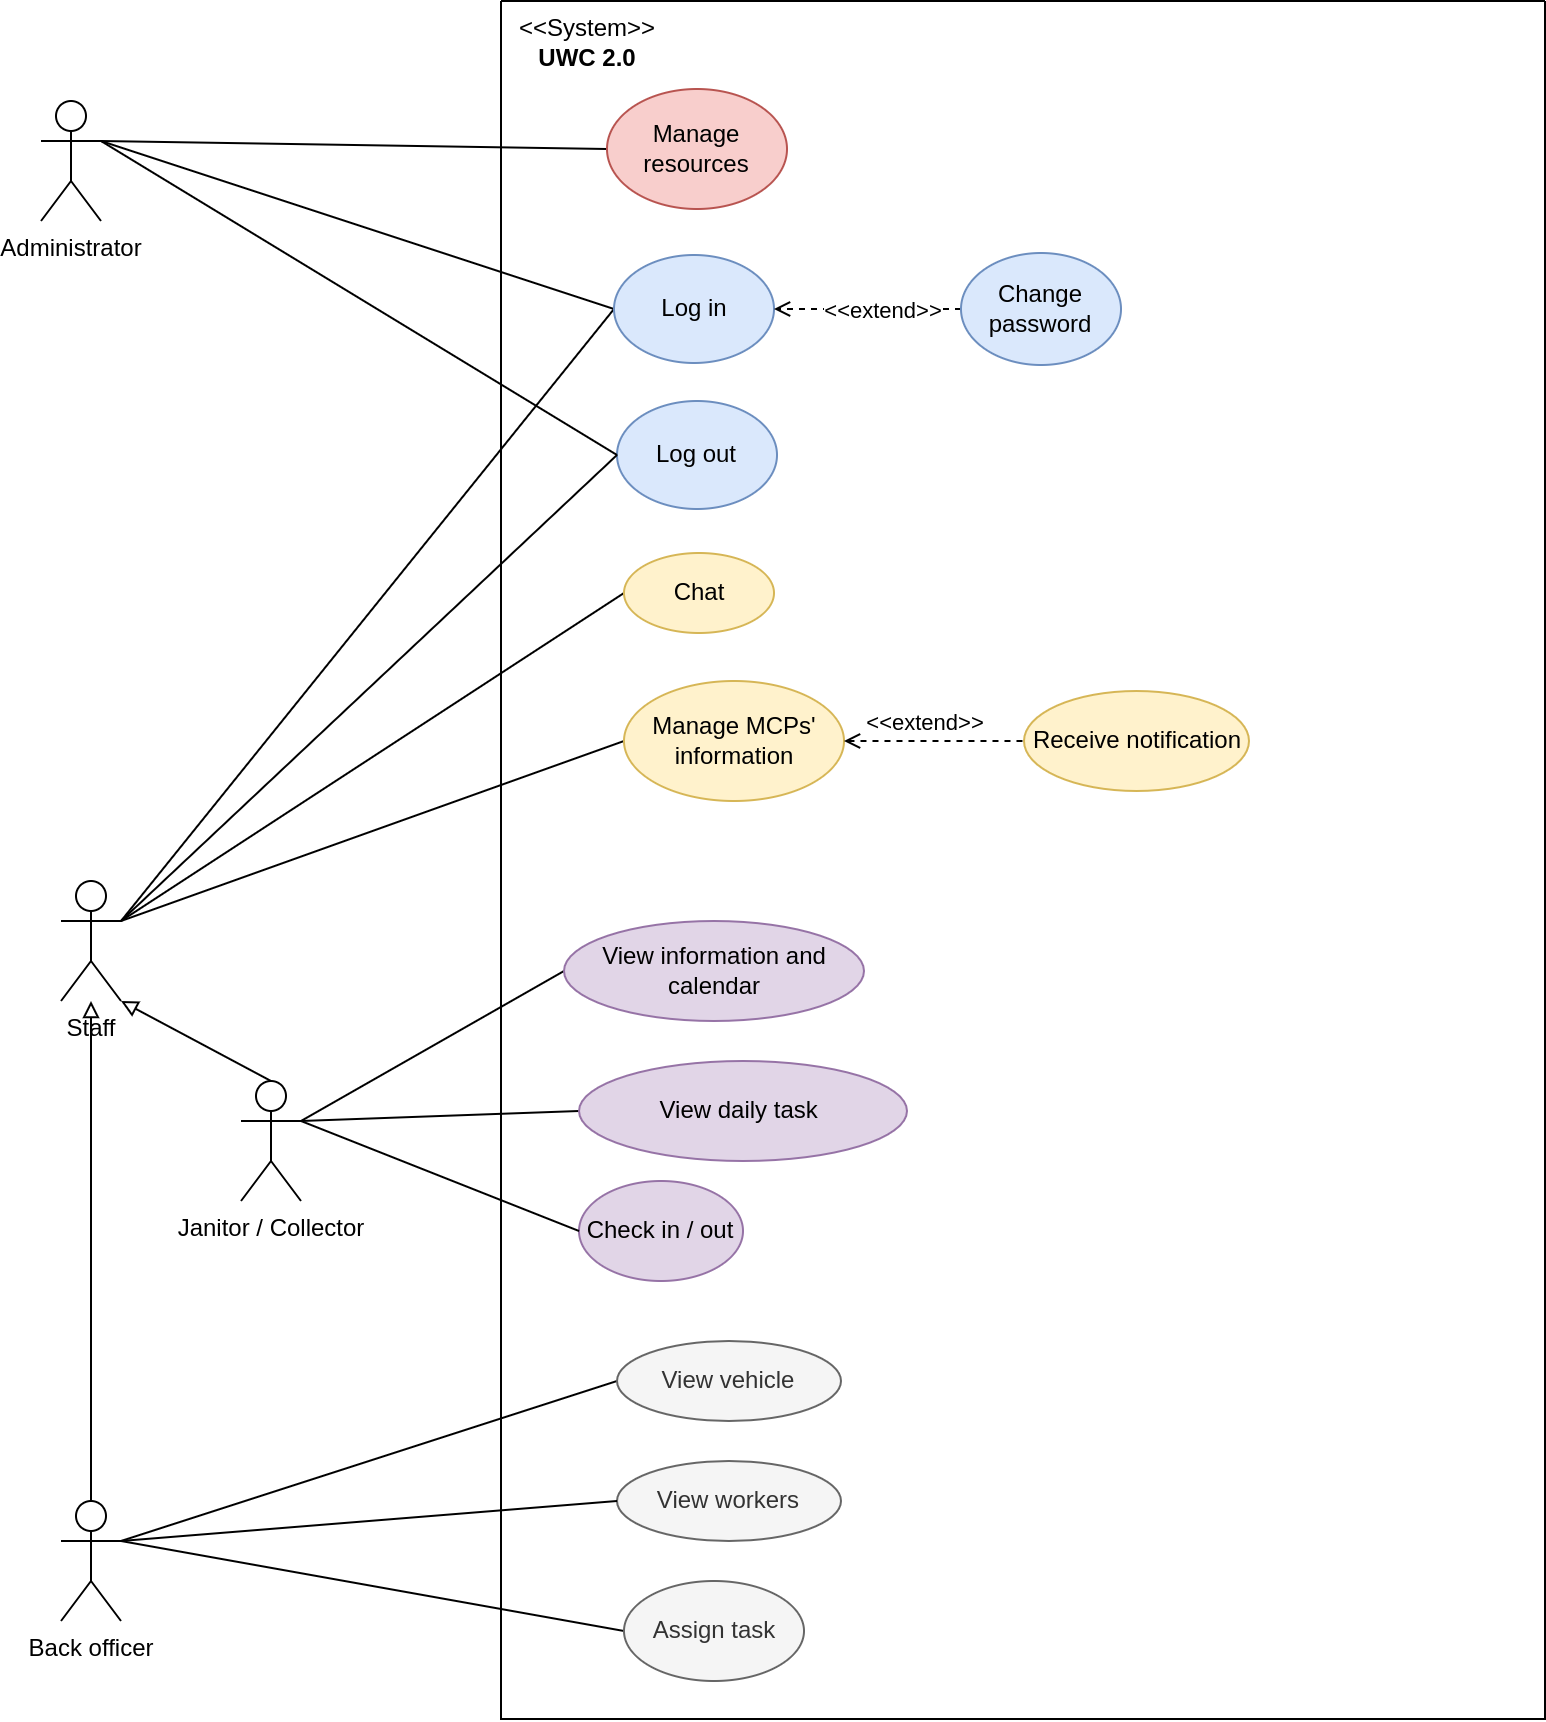
\includegraphics[width=0.93\linewidth]{imgs/use-case diagram/main_uc.png}
        \caption{Use-case diagram tổng quát của hệ thống}
    \end{figure}

    \begin{tblr}{
        width=1\linewidth,
        hlines,
        vlines,
        colspec={X[3]X[7]},
        columns = {valign = m, },
        row{1} = {halign = c, valign = m, bg = lightgray, fg = black},
    }
        {\textbf{Use case name} & \textbf{Manage resources}}  \\
        Description	& Quản lý tài nguyên của công ty \\
        Actor & Người quản lý (Administrator) \\
        Trigger & Người quản lý ấn vào phần quản lý tài nguyên  \\
        Pre-condition & Người quản lý đã đăng nhập và đang ở màn hình chính\\
        Post-condition & Người quản lý được đưa vào trang quản lý tài nguyên\\
        Normal flow &   		1. Hệ thống hiển thị giao diện quản lý tài nguyên \newline
                                2. Quản lý thực hiện việc quản lý tài nguyên \\
        Alternative flow  & 	none \\
        Exception flow & none\\
    \end{tblr}

    \vspace{1cm}

    \begin{tblr}{
        width=1\linewidth,
        hlines,
        vlines,
        colspec={X[3]X[7]},
        columns = {valign = m, },
        row{1} = {halign = c, valign = m, bg = lightgray, fg = black},
    }
        {\textbf{Use case name} & \textbf{Log in}}  \\
        Description	& Đăng nhập vào hệ thống \\
        Actor & Người quản lý (Administrator), nhân viên giám sát (Back officer), nhân viên lái xe rác (Collector), nhân viên thu gom rác (Janitor) \\
        Trigger & Người dùng mở ứng dụng  \\
        Pre-condition & Thiết bị phải có kết nối Internet\\
        Post-condition & Người dùng đăng nhập thành công\\
        Normal flow &   1. Hệ thống hiển thị giao diện đăng nhập \newline
                    	2. Người dùng ghi thông tin về tên tài khoản và mật khẩu \newline
                    	3. Hệ thống kiểm tra thông tin được ghi \newline
                    	4. Hệ thống thông báo đăng nhập thành công \newline
                    	5. Hệ thống hiển thị giao diện màn hình chính \\
        Alternative flow  & Alternative flow thứ 1: tại bước 2 \newline
                        	1a. Người dùng chọn lưu tài khoản \newline
                        	Tiếp tục bước 3 \newline
                        	1b. Hệ thống lưu lại tài khoản \newline
                        	Tiếp tục bước 4 \\
        Exception flow & 	Exception flow thứ 1: tại bước 3 \newline
                        	1a. Nếu không tìm thấy tài khoản, sai mật khẩu, thông báo cho người dùng \newline
                        	Quay lại bước 2 \\
        Extended points & Change password \\
    \end{tblr}

    \vspace{1cm}
    \begin{tblr}{
        width=1\linewidth,
        hlines,
        vlines,
        colspec={X[3]X[7]},
        columns = {valign = m, },
        row{1} = {halign = c, valign = m, bg = lightgray, fg = black},
    }
        {\textbf{Use case name} & \textbf{Change password}}  \\
        Description	& Thay đổi mật khẩu của tài khoản \\
        Actor & Người quản lý (Administrator), nhân viên giám sát (Back officer), nhân viên lái xe rác (Collector), nhân viên thu gom rác (Janitor) \\
        Trigger & Người dùng ấn vào nút quên mật khẩu  \\
        Pre-condition & Người dùng đang ở phần đăng nhập \\
        Post-condition & Mật khẩu được thay đổi thành công \\
        Normal flow &   1. Hệ thống hiển thị thay giao diện thay đổi mật khẩu \newline
                    	2. Người dùng nhập tên tài khoản \newline
                    	3. Hệ thống kiểm tra tài khoản \newline
                    	4. Người dùng nhập mã mật khẩu mới \newline
                    	5. Hệ thống kiểm tra mật khẩu mới \newline
                    	6. Hệ thống thông báo đổi mật khẩu thành công \newline
                    	7. Hệ thống quay lại trang đăng nhập \\
        Alternative flow  & none \\
        Exception flow & 	Exception flow thứ 1: tại bước 3 \newline
                            1a. Nếu tài khoản không tồn tại, thông báo cho người dùng \newline
                            Quay lại bước 2 \newline

                            Exception flow thứ 2: tại bước 5 \newline
                            2a. Nếu mật khẩu không đúng quy đinh, thông báo cho người dùng \newline
                            Quay lại bước 4 \\
    \end{tblr}

    \vspace{1cm}
    \begin{tblr}{
        width=1\linewidth,
        hlines,
        vlines,
        colspec={X[3]X[7]},
        columns = {valign = m, },
        row{1} = {halign = c, valign = m, bg = lightgray, fg = black},
    }
        {\textbf{Use case name} & \textbf{Log out}}  \\
        Description	& Đăng xuất khỏi phiên làm việc \\
        Actor & Người quản lý (Administrator), nhân viên giám sát (Back officer), nhân viên lái xe rác (Collector), nhân viên thu gom rác (Janitor) \\
        Trigger & Người dùng ấn vào nút đăng xuất  \\
        Pre-condition & Người dùng đã đăng nhập, và đang ở màn hình chính \\
        Post-condition & Tài khoản được đăng xuất khỏi hệ thống \\
        Normal flow &   1. Người dùng ấn vào menu \newline
                    	2. Người dùng chọn đăng xuất \newline
                    	3. Hệ thống hiện thị form xác nhận đăng xuất \newline
                    	4. Hệ thống xóa phiên làm việc  \newline
                    	5. Hệ thống quay trở lại trang đăng nhập \\
        Alternative flow  & Alternative flow thứ 1: tại bước 3 \newline
                            1a. Nếu người dùng chọn hủy, quay lại màn hình chính \\
        Exception flow & none\\
    \end{tblr}

    \begin{tblr}{
        width=1\linewidth,
        hlines,
        vlines,
        colspec={X[3]X[7]},
        columns = {valign = m, },
        row{1} = {halign = c, valign = m, bg = lightgray, fg = black},
    }
        {\textbf{Use case name} & \textbf{Chat}}  \\
        Description	& Nhân viên liên lạc với nhau \\
        Actor & Nhân viên (Staff) \\
        Trigger & 	Nhân viên ấn vào phần liên hệ \\
        Pre-condition & Người dùng đã đăng nhập\\
        Post-condition & Tin nhắn được gửi thành công \newline
                         Nhân viên nhận và đọc được tin nhắn \\
        Normal flow &   1. Hệ thống lấy thông tin về các nhân viên \newline
                    	2. Hệ thống hiển thị danh sách các nhân viên \newline
                    	3. Người dùng chọn nhân viên muốn liên hệ \newline
                    	4. Hệ thống hiển thị giao diện nhắn tin \newline
                    	5. Người dùng nhập tin nhắn \newline
                    	6. Người dùng nhấn gửi \newline
                    	7. Hệ thống ghi nhận tin nhắn và gửi cho người được nhắn \\
        Alternative flow  & none \\
        Exception flow & none \\
    \end{tblr}

    \vspace{1cm}
    \begin{tblr}{
        width=1\linewidth,
        hlines,
        vlines,
        colspec={X[3]X[7]},
        columns = {valign = m, },
        row{1} = {halign = c, valign = m, bg = lightgray, fg = black},
    }
        {\textbf{Use case name} & \textbf{Manage MCP's information}}  \\
        Description	& Xem thông tin về các MCPs \\
        Actor & Nhân viên (Staff) \\
        Trigger & 	Nhân viên ấn vào mục tổng quan MCPs \\
        Pre-condition & Nhân viên đã đăng nhập và đang ở màn hình chính \\
        Post-condition & Thông tin về MCP được hiển thị thành công \\
        Normal flow &   1. Hệ thống lấy thông tin các MCPs \newline
                    	2. Hệ thống hiện thị danh sách các MCPs \newline
                    	3. Nhân viên chọn 1 MCP bất kì \newline
                    	4. Hệ thống hiển thị thông tin chi tiết của MCPs vừa được chọn \\
        Alternative flow  & none \\
        Exception flow & none \\
        Extended points & Receive notification \\
    \end{tblr}

    \begin{tblr}{
        width=1\linewidth,
        hlines,
        vlines,
        colspec={X[3]X[7]},
        columns = {valign = m, },
        row{1} = {halign = c, valign = m, bg = lightgray, fg = black},
    }
        {\textbf{Use case name} & \textbf{Receive notification}}  \\
        Description	& Cập nhật tình trạng của MCP \\
        Actor & Nhân viên (Staff) \\
        Trigger & none \\
        Pre-condition & Nhân viên đã đăng nhập \\
        Post-condition & Thông báo được nhận bởi nhân viên \\
        Normal flow &   1. Hệ thống truy cập vào dữ liệu về MCPs \newline
                    	2. Hệ thống lấy thông tin về dung tích của MCPs \newline
                    	3. Hệ thống gửi thông báo về cho người dùng \newline
                    	4. Người dùng nhận được thông báo \\
        Alternative flow  & none \\
        Exception flow & none \\
    \end{tblr}

    \vspace{1cm}
    \begin{tblr}{
        width=1\linewidth,
        hlines,
        vlines,
        colspec={X[3]X[7]},
        columns = {valign = m, },
        row{1} = {halign = c, valign = m, bg = lightgray, fg = black},
    }
        {\textbf{Use case name} & \textbf{View information and calendar}}  \\
        Description	& Công nhân xem thông tin và lịch làm trong tuần \\
        Actor & 	Nhân viên lái xe rác (Collector), Nhân viên thu gom rác (Janitor) \\
        Trigger & 	Công nhân ấn vào phần thông tin và lịch làm \\
        Pre-condition & Công nhân đã đăng nhập và đang ở màn hình chính \\
        Post-condition & Công nhân xem được thông tin và lịch làm của mình \\
        Normal flow &   1. Hệ thống lấy thông tin và lịch làm \newline
                    	2. Hệ thống hiển thị giao diện bao gồm 2 tab (thông tin chung, lịch làm) 	mặc định ở thông tin chung \newline
                    	3. Công nhân xem thông tin của bản thân\\
        Alternative flow  & Alternative flow thứ 1: Tại bước 2 \newline
                    	    1a. Người dùng chọn tab lịch làm \newline
                    	    1b. Hệ thống hiển thị giao diện về lịch làm việc trong tuần \\
        Exception flow & none \\
    \end{tblr}

    \begin{tblr}{
        width=1\linewidth,
        hlines,
        vlines,
        colspec={X[3]X[7]},
        columns = {valign = m, },
        row{1} = {halign = c, valign = m, bg = lightgray, fg = black},
    }
        {\textbf{Use case name} & \textbf{View daily task}}  \\
        Description	& Công nhân xem chi tiết công việc trong ngày \\
        Actor & 	Nhân viên lái xe rác (Collector), Nhân viên thu gom rác (Janitor) \\
        Trigger & 	Công nhân ấn vào phần nhiệm vụ hôm nay\\
        Pre-condition & Công nhân đã đăng nhập và đang ở màn hình chính \\
        Post-condition & Nhiệm vụ cụ thể trong ngày được hiện lên màn hình \\
        Normal flow &   1. Hệ thống lấy thông tin làm việc trong ngày \newline
                    	2. Hệ thống hiển thị thông tin làm việc \newline
                    	3. Người dùng đọc được thông tin làm việc\\
        Alternative flow  & none \\
        Exception flow & none \\
    \end{tblr}

    \vspace{1cm}
    \begin{tblr}{
        width=1\linewidth,
        hlines,
        vlines,
        colspec={X[3]X[7]},
        columns = {valign = m, },
        row{1} = {halign = c, valign = m, bg = lightgray, fg = black},
    }
        {\textbf{Use case name} & \textbf{Check in/out}}  \\
        Description	& Nhận và đánh dấu hoàn thành công việc \\
        Actor & 	Nhân viên lái xe rác (Collector), Nhân viên thu gom rác (Janitor) \\
        Trigger & 		Công nhân chọn nhận công việc \\
        Pre-condition & Công nhân đang ở phần thông tin nhiệm vụ chi tiết \\
        Post-condition & Nhiệm vụ được nhận / được hoàn thành \\
        Normal flow &   1. Công nhân xác nhận nhiệm vụ \newline
                        2. Hệ thống ghi nhận công nhân đã xác nhận \\
        Alternative flow  & Alternative flow thứ 1: tại bước 1 \newline
                        	1a. Công nhân ấn hoàn thành nhiệm vụ \newline
                        	1b. Hệ thống ghi nhận \\
        Exception flow & none \\
    \end{tblr}

    \begin{tblr}{
        width=1\linewidth,
        hlines,
        vlines,
        colspec={X[3]X[7]},
        columns = {valign = m, },
        row{1} = {halign = c, valign = m, bg = lightgray, fg = black},
    }
        {\textbf{Use case name} & \textbf{View workers}}  \\
        Description	& Xem thông tin công nhân và lịch làm của họ \\
        Actor & 	Nhân viên giám sát (Back officer) \\
        Trigger & 	Nhân viên giám sát ấn vào mục quản lý nhân viên \\
        Pre-condition & Nhân viên giám sát đã đăng nhập và đang ở màn hình chính \\
        Post-condition & Thông tin chi tiết và lịch làm việc trong tuần của công nhân được hiển thị \\
        Normal flow &   1. Hệ thống lấy dữ liệu của nhân viên \newline
                    	2. Hệ thống hiển thị danh sách tên các nhân viên \newline
                    	3. Nhân viên giám sát chọn một nhân viên \newline
                    	4. Hệ thống hiển thị thông tin chi tiết của nhân viên \\
        Alternative flow  & Alternative flow thứ 1: tại bước 4 \newline
                        	1a. Người dùng chọn qua mục lịch làm việc \newline
                        	1b. Hệ thống lấy thông tin về lịch làm việc của nhân viên \newline
                        	1c. Hệ thống hiển thị lên màn hình \\
        Exception flow & none \\
    \end{tblr}

    \vspace{1cm}
    \begin{tblr}{
        width=1\linewidth,
        hlines,
        vlines,
        colspec={X[3]X[7]},
        columns = {valign = m, },
        row{1} = {halign = c, valign = m, bg = lightgray, fg = black},
    }
        {\textbf{Use case name} & \textbf{View vehicle}}  \\
        Description	& Xem thông tin của các phương tiện \\
        Actor & 	Nhân viên giám sát (Back officer) \\
        Trigger & 	Nhân viên giám sát ấn vào mục theo dõi phương tiện\\
        Pre-condition & Nhân viên giám sát đã đăng nhập và đang ở màn hình chính \\
        Post-condition & Thông tin phương tiện được hiển thị trên màn hình \\
        Normal flow &   1. Hệ thống truy cập vào dữ liệu về phương tiện \newline
                    	2. Hệ thống hiển thị các phương tiện \newline
                    	3. Người dùng chọn một phương tiện bất kì \newline
                    	4. Hệ thống hiện thị thông tin chi tiết của phương tiện \\
        Alternative flow  & none \\
        Exception flow & none \\
    \end{tblr}
    \newpage

    
\subsection{Chức năng phân chia công việc (Task assignment)}
    \begin{figure}[h]
        \centering
        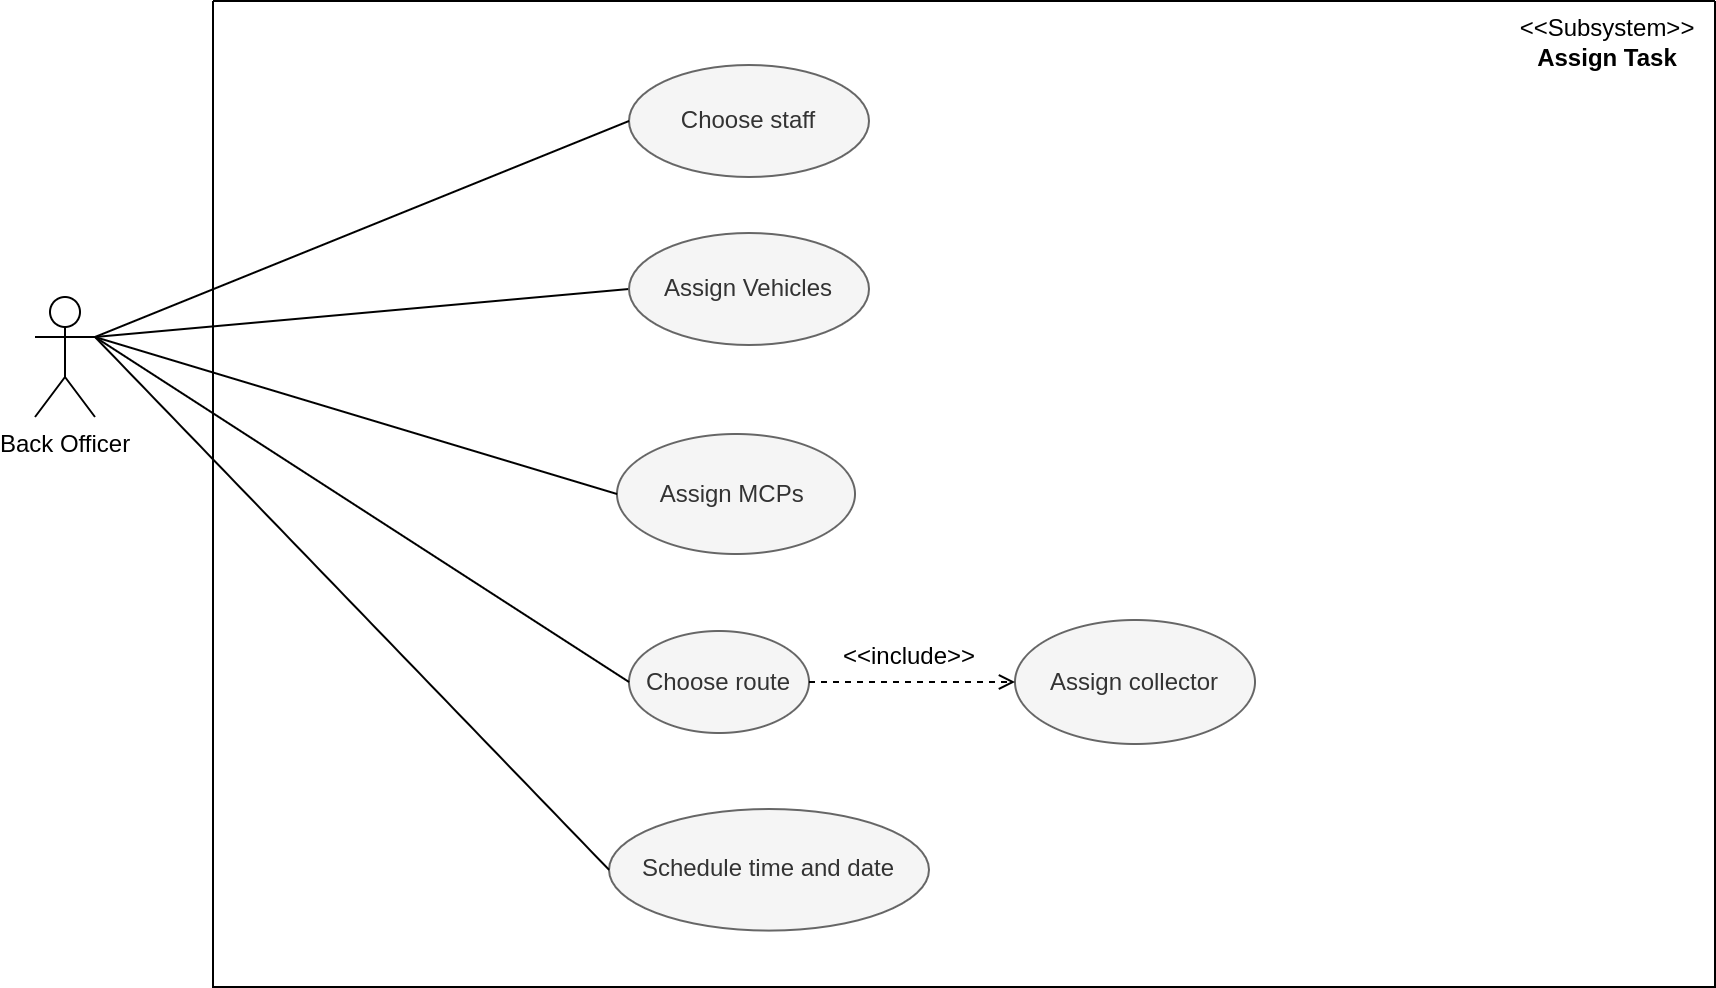
\includegraphics[width=1\linewidth]{imgs/use-case diagram/assignTask_uc.png}
        \caption{Use-case diagram chức năng phân chia công việc}
    \end{figure}

    \vspace{1cm}
    \begin{tblr}{
        width=1\linewidth,
        hlines,
        vlines,
        colspec={X[3]X[7]},
        columns = {valign = m, },
        row{1} = {halign = c, valign = m, bg = lightgray, fg = black},
    }
        {\textbf{Use case name} & \textbf{Choose staff}}  \\
        Description	& Chọn một nhân viên trong hệ thống \\
        Actor & 	Nhân viên giám sát (Back officer) \\
        Trigger & 		Nhân viên giám sát ấn nút chọn công nhân\\
        Pre-condition & Nhân viên giám sát đang ở phần phân công công việc \\
        Post-condition & Công nhân được chọn \\
        Normal flow &   1. Hệ thống lấy dữ liệu về công nhân \newline
                    	2. Hệ thống hiển thị các công nhân \newline
                    	3. Nhân viên giám sát chọn công nhân \newline
                    	4. Hệ thống ghi nhận công nhân được chọn \\
        Alternative flow  & none \\
        Exception flow & none \\
    \end{tblr}

    \begin{tblr}{
        width=1\linewidth,
        hlines,
        vlines,
        colspec={X[3]X[7]},
        columns = {valign = m, },
        row{1} = {halign = c, valign = m, bg = lightgray, fg = black},
    }
        {\textbf{Use case name} & \textbf{Choose vehicle}}  \\
        Description	& Chọn một phương tiện có trong công ty \\
        Actor & 	Nhân viên giám sát (Back officer) \\
        Trigger & 		Nhân viên giám sát ấn nút chọn công nhân\\
        Pre-condition & Nhân viên giám sát đang ở phần phân công công việc \\
        Post-condition & Phương tiện được chọn thành công \\
        Normal flow &   1. Hệ thống lấy dữ liệu về phương tiện \newline
                    	2. Hệ thống hiển thị các phương tiện \newline
                    	3. Nhân viên giám sát chọn phương tiện \newline
                    	4. Hệ thống kiểm tra phương tiện đã được lái hay chưa \newline
                    	5. Hệ thống ghi nhận phương tiện được chọn \\
        Alternative flow  & none \\
        Exception flow & Exception flow thứ 1: tại bước 4 \newline
                    	 1a. Nếu phương tiện đã được gán, thông báo cho người dùng \newline
                    	 Quay lại bước 2 \\
    \end{tblr}

    \vspace{1cm}
    \begin{tblr}{
        width=1\linewidth,
        hlines,
        vlines,
        colspec={X[3]X[7]},
        columns = {valign = m, },
        row{1} = {halign = c, valign = m, bg = lightgray, fg = black},
    }
        {\textbf{Use case name} & \textbf{Assign MCPs}}  \\
        Description	& Gán các điểm MCP cho công nhân \\
        Actor & 	Nhân viên giám sát (Back officer) \\
        Trigger & 	Nhân viên giám sát ấn nút chọn MCPs\\
        Pre-condition & Người quản lý đang ở phần phân công công việc \\
        Post-condition & Các điểm MCP được phân công thành công\\
        Normal flow &   1. Hệ thống lấy dữ liệu về các MCP \newline
                    	2. Hệ thống hiển thị các MCP \newline
                    	3. Nhân viên giám sát chọn MCP \newline
                    	4. Hệ thống ghi nhận các MCP được chọn \\
        Alternative flow  & Alternative flow thứ 1: tại bước 3 \newline
                        	1a. Nếu công nhân được chọn là collector, cho phép gán nhiều MCP \newline
                            \newline
                        	Alternative flow thứ 2: tại bước 3 \newline
                        	2a. Nếu công nhân được chọn là janitor, cho phép gán chỉ 1 MCP \\
        Exception flow & none \\
    \end{tblr}

    \begin{tblr}{
        width=1\linewidth,
        hlines,
        vlines,
        colspec={X[3]X[7]},
        columns = {valign = m, },
        row{1} = {halign = c, valign = m, bg = lightgray, fg = black},
    }
        {\textbf{Use case name} & \textbf{Choose route}}  \\
        Description	& Chọn tuyến đường cho collector \\
        Actor & 	Nhân viên giám sát (Back officer) \\
        Trigger & 	Nhân viên giám sát ấn nút chọn tuyến đường \\
        Pre-condition & Người quản lý đang ở phần phân công công việc \\
        Post-condition & Tuyến đường được chọn\\
        Normal flow &   1. Hệ thống kiểm tra công nhân được chọn là ai \newline
                    	2. Hệ thống hiển thị map trong thành phố \newline
                    	3. Hệ thống hiển thị các tuyến đường được xem là tối ưu \newline
                    	4. Nhân viên giám sát chọn tuyến đường \newline
                    	5. Hệ thống ghi nhận tuyến đường được chọn \\
        Alternative flow  & Alternative flow thứ 1: tại bước 1 \newline
                            1a. Nếu công nhân được chọn là Janitor, hệ thống thông báo và quay 	trở lại màn hình phân công công việc \\
        Exception flow & none \\
    \end{tblr}

    \vspace{1cm}
    \begin{tblr}{
        width=1\linewidth,
        hlines,
        vlines,
        colspec={X[3]X[7]},
        columns = {valign = m, },
        row{1} = {halign = c, valign = m, bg = lightgray, fg = black},
    }
        {\textbf{Use case name} & \textbf{Schedule time and date}}  \\
        Description	& Xếp lịch cho nhân viên \\
        Actor & 	Nhân viên giám sát (Back officer) \\
        Trigger & 	Nhân viên giám sát ấn nút set lịch làm\\
        Pre-condition & Người quản lý đang ở phần phân công công việc \\
        Post-condition & Lịch làm được phân thành công\\
        Normal flow &   1. Hệ thống lấy dữ liệu về lịch làm \newline
                    	2. Hệ thống hiển thị các ngày trong tuần \newline
                    	3. Nhân viên giám sát chọn các ca còn trống \newline
                    	4. Nhân viên xác nhận lịch đã chọn \newline
                    	5. Hệ thống ghi nhận lịch làm \\
        Alternative flow  & none \\
        Exception flow & none \\
    \end{tblr}

\newpage

    

\subsection{Chức năng quản lý tài nguyên (Manage Resources)}
    \begin{figure}[h]
        \centering
        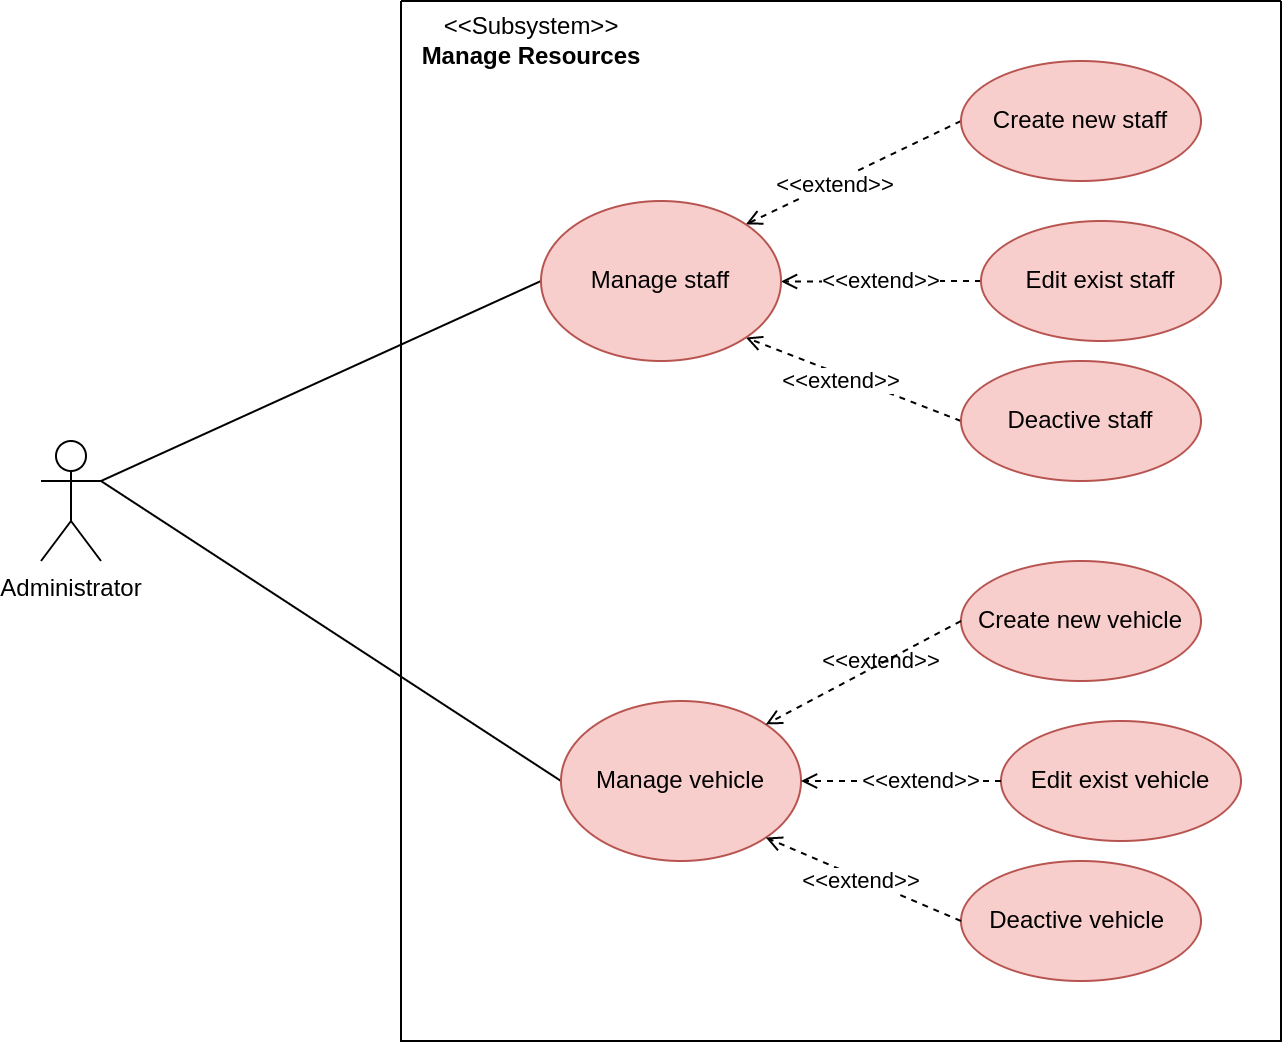
\includegraphics[width=0.70\linewidth]{imgs/use-case diagram/manageResources_uc.png}
        \caption{Use-case diagram chức năng kiểm soát tài nguyên}
    \end{figure}

    \vspace{1cm}
    \begin{tblr}{
        width=1\linewidth,
        hlines,
        vlines,
        colspec={X[3]X[7]},
        columns = {valign = m, },
        row{1} = {halign = c, valign = m, bg = lightgray, fg = black},
    }
        {\textbf{Use case name} & \textbf{Manage staff}}  \\
        Description	& Xếp lịch cho nhân viên \\
        Actor & 	Người quản lý (Administrator) \\
        Trigger & 	Người quản lý ấn vào phần quản lý nhân viên ở menu chính \\
        Pre-condition & Người quản lý đang ở quản lý tài nguyên \\
        Post-condition & Trang quản lý nhân viên được hiển thị \\
        Normal flow &   1. Hệ thống lấy dữ liệu về các nhân viên\newline
                    	2. Hệ thống hiện thị danh sách nhân viên lên màn hình \newline
                    	3. Người dùng chọn một nhân viên để thực hiện hành động \newline
                     	4. Hệ thống hiện thị thông tin chi tiết của nhân viên \\
        Extended points & 	Create new staff \newline
                        	Edit exist staff \newline
                        	Deactive staff \\
    \end{tblr}

    \begin{tblr}{
        width=1\linewidth,
        hlines,
        vlines,
        colspec={X[3]X[7]},
        columns = {valign = m, },
        row{1} = {halign = c, valign = m, bg = lightgray, fg = black},
    }
        {\textbf{Use case name} & \textbf{Create new staff}}  \\
        Description	& Tạo ra một nhân viên mới \\
        Actor & 	Người quản lý (Administrator) \\
        Trigger & 	Người quản lý ấn vào nút tạo người dùng mới \\
        Pre-condition & Người quản lý đang ở trong phần quản lý nhân viên \\
        Post-condition & Nhân viên mới được tạo ra \\
        Normal flow &   1. Hệ thống hiển thị các thông tin cần điền \newline
                    	2. Người dùng điền các thông tin \newline
                    	3. Hệ thống kiểm tra thông tin được điền \newline
                    	4. Người dùng ấn tạo nhân viên mới \newline
                    	5. Hệ thống ghi nhận nhân viên mới \newline
                    	6. Hệ thống thông báo tạo nhân viên thành công \\
        Alternative flow  & Alternative flow thứ 1: tại bước 1 \newline
                        	1a. Người dùng ấn nút hủy \newline
                        	1b. Quay lại màn hình thông tin chi tiết của nhân viên \\
        Exception flow & Exception flow thứ 1: tại bước 3 \newline
                    	 1a. Nếu thông tin sai, thông báo cho người dùng \newline
                    	 Quay lại bước 2  \\
    \end{tblr}

    \vspace{1cm}
    \begin{tblr}{
        width=1\linewidth,
        hlines,
        vlines,
        colspec={X[3]X[7]},
        columns = {valign = m, },
        row{1} = {halign = c, valign = m, bg = lightgray, fg = black},
    }
        {\textbf{Use case name} & \textbf{Edit exist staff}}  \\
        Description	& Chỉnh sửa một nhân viên  \\
        Actor & 	Người quản lý (Administrator) \\
        Trigger & 	Người quản lý ấn vào nút chỉnh sửa nhân viên \\
        Pre-condition & Người quản lý đang ở trong phần quản lý nhân viên \\
        Post-condition & Thông tin nhân viên được chỉnh sửa thành công\\
        Normal flow &   1. Hệ thống hiển thị các thông tin cần điền \newline
                    	2. Người dùng điền các thông tin \newline
                    	3. Hệ thống kiểm tra thông tin được điền \newline
                    	4. Người dùng ấn cập nhật nhân viên \newline
                    	5. Hệ thống ghi nhận thông tin được cập nhật \newline
                    	6. Hệ thống thông báo cập nhật nhân viên thành công \\
        Alternative flow  & Alternative flow thứ 1: tại bước 1 \newline
                        	1a. Người dùng ấn nút hủy \newline
                        	1b. Quay lại màn hình thông tin chi tiết của nhân viên \\
        Exception flow & Exception flow thứ 1: tại bước 3 \newline
                    	 1a. Nếu thông tin sai, thông báo cho người dùng \newline
                    	 Quay lại bước 2 \\
    \end{tblr}

    \begin{tblr}{
        width=1\linewidth,
        hlines,
        vlines,
        colspec={X[3]X[7]},
        columns = {valign = m, },
        row{1} = {halign = c, valign = m, bg = lightgray, fg = black},
    }
        {\textbf{Use case name} & \textbf{Deactive staff}}  \\
        Description	& Hủy kích hoạt một nhân viên \\
        Actor & 	Người quản lý (Administrator) \\
        Trigger & 	Người quản lý ấn vào nút hủy kích hoạt nhân viên \\
        Pre-condition & Người quản lý đang ở trong phần quản lý nhân viên \\
        Post-condition & Nhân viên bị hủy kích hoạt\\
        Normal flow &   1. Hệ thống hiểu thị xác nhận hủy kích hoạt nhân viên \newline
                    	2. Người dùng nhấn đồng ý \newline
                    	3. Hệ thống hủy kích hoạt nhân viên \newline
                    	4. Hệ thống thông báo hủy kích hoạt thành công \\
        Alternative flow  & Alternative flow thứ 1: tại bước 1 \newline
                        	1a. Người dùng ấn nút hủy \newline
                        	1b. Quay lại màn hình thông tin chi tiết của nhân viên \\
        Exception flow & none \\
    \end{tblr}

    \vspace{1cm}
    \quad Phần use-case senario của  Manage vehicle tương tự như trên.


	
\section{Activity diagram giữa hệ thống và các bên liên quan trong Task Assignment Module}
    \begin{figure}[h]
        \centering
        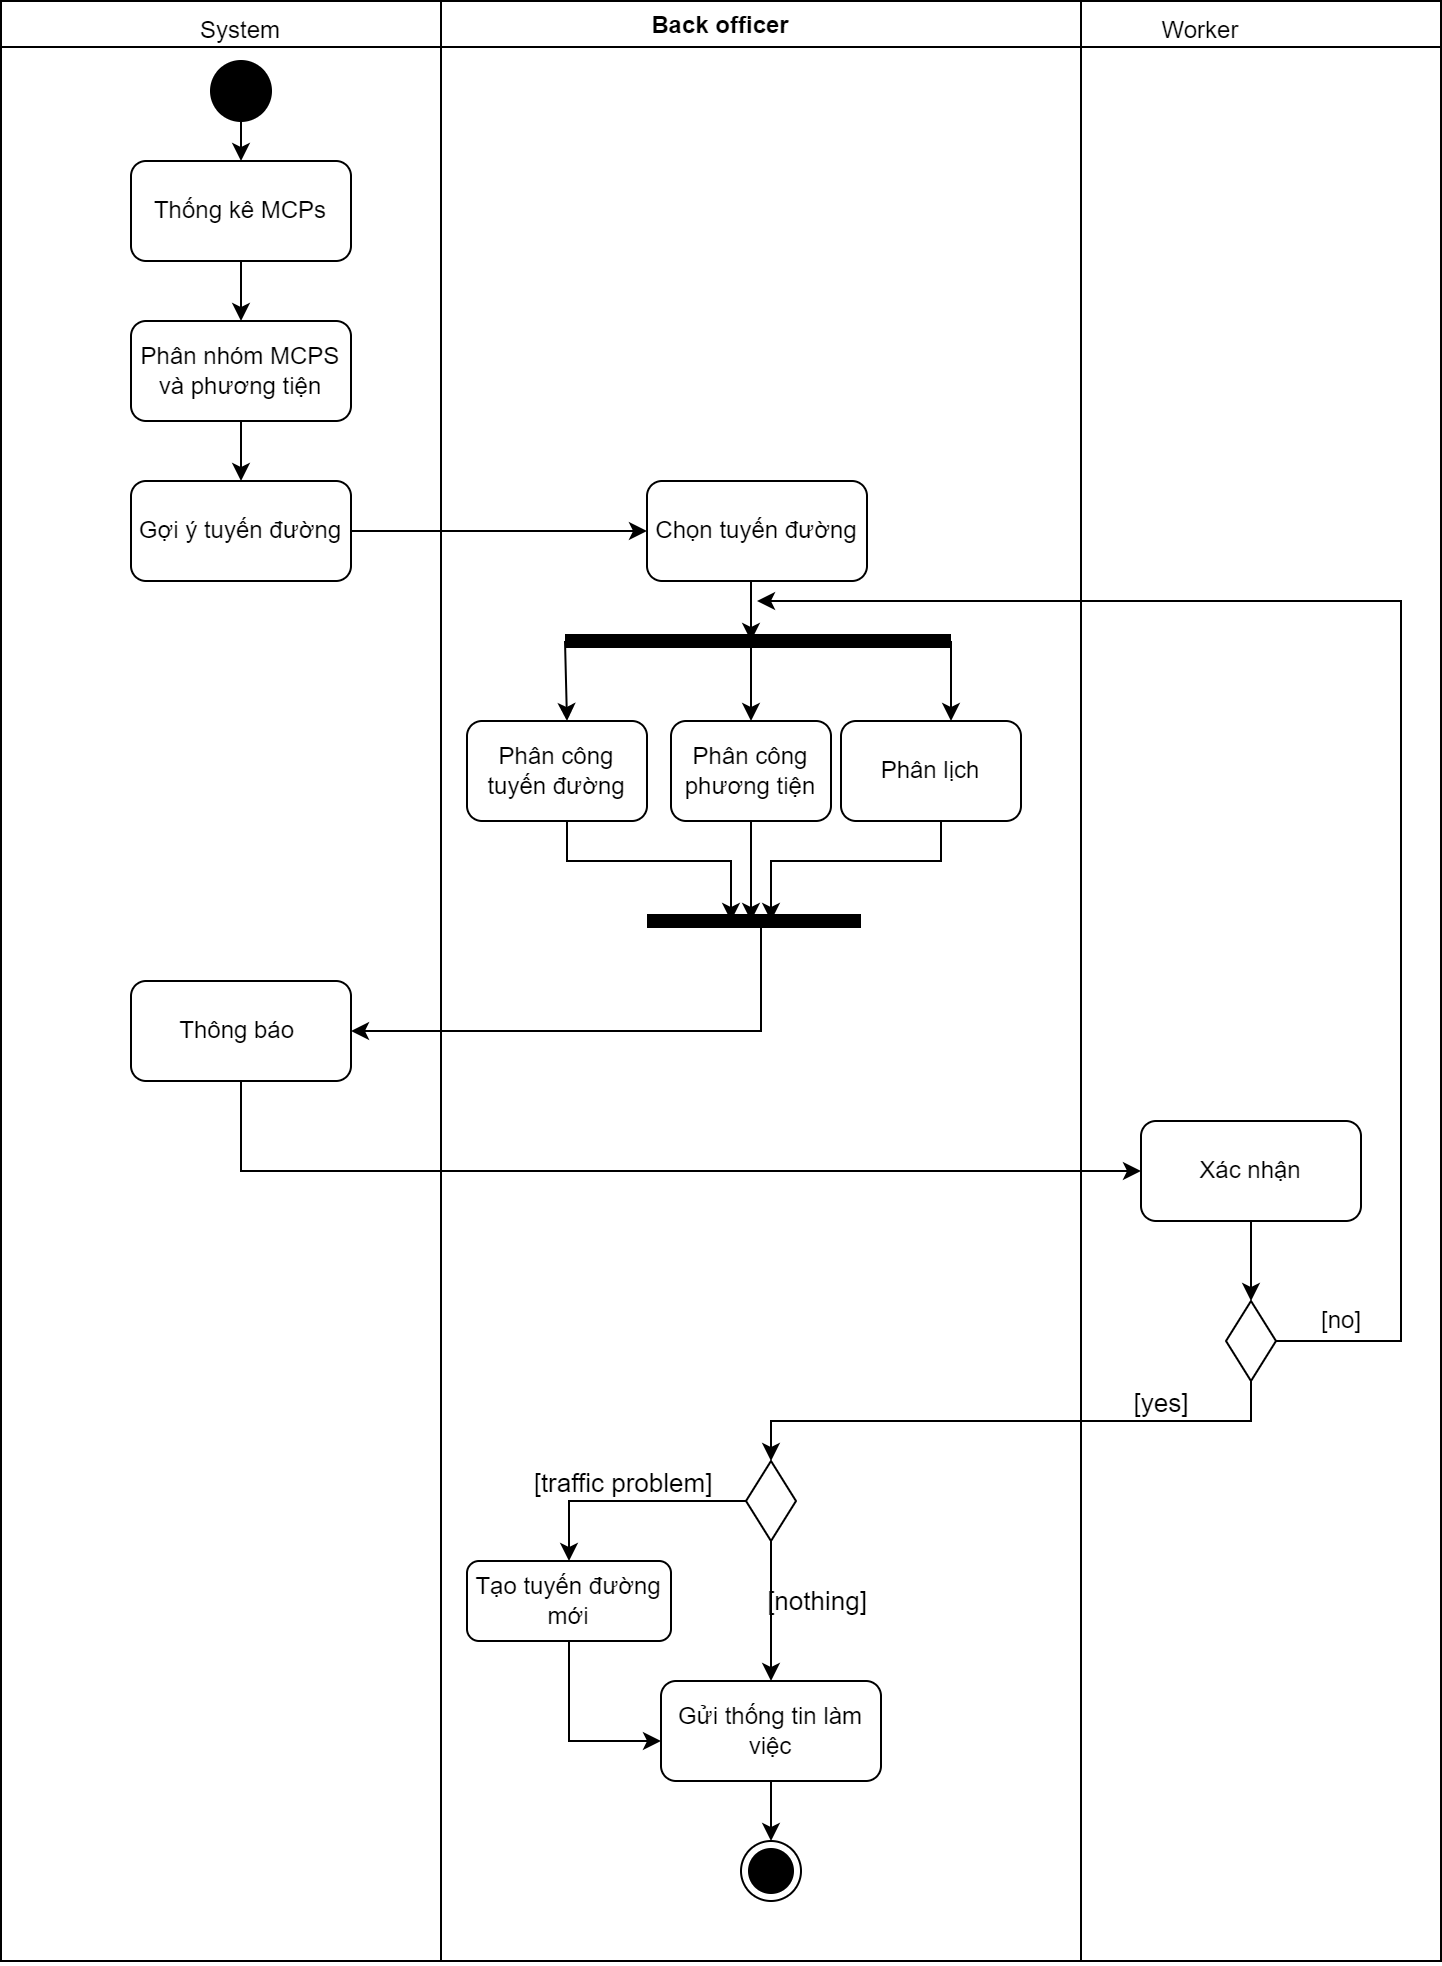
\includegraphics[width=15.0cm,height=15cm]{imgs/activity diagram/activity diagram.png}
        \caption{Activity diagram trong Task Asssignment Module}
    \end{figure}
    \newpage
    Hoạt động giữa hệ thống và các bên liên quan trong Task Assignment Module gồm các hoạt động theo thứ tự:
    \begin{enumerate}
        \item Bắt đầu.
        \item Hệ thống thống kê số lượng, vị trí MCPs.
        \item Hệ thống phân nhóm MCPs theo vùng phù hợp với sức chứa của phương tiện hiện có để tối ưu về tuyến đường và nhiên liệu.
        \item Hệ thống gợi ý các tuyến đường tối ưu cho Back officer.
        \item Back officer chọn tuyến đường cho tháng.
        \item Back officer phân công tuyến đường, phân phương tiện và tạo lịch cho collectors, janitors.
        \item Hệ thống gửi thông báo cho collectors, janitors.
        \item  Collectors, janitors xem thông báo được gửi.
        \item Back officer gửi thông tin làm việc theo ngày cho collectors, janitors.
        \item Kết thúc
    \end{enumerate}

\section{Giải pháp ý niệm cho task Route planning và Sequence diagram mô tả nó}
    \subsection{Giải pháp ý niệm cho task Route Planning}
        \textbf{Xét các Actor: }
    
        \begin{itemize}
            \item[-] Back Officer.
            \item[-] Cơ sở dữ liệu bản đồ (Map Database): một API cung cấp mọi thông tin về đường đi trong một vùng không gian nhất định khi được yêu cầu.
        \end{itemize}
    
        \textbf{Giả định:}
    
        \begin{itemize}
            \item[-] Back Officer đã đăng nhập thành công vào hệ thống.
            \item[-] Back Officer đã thao tác với hệ thống, đã nạp một danh sách các MCPs mà mình có nhu cầu tìm đường.
            \item[-] Map Database luôn hoạt động và hoạt động đúng kỳ vọng.
        \end{itemize}
    
        \textbf{Ta có, các entity liên quan:}
    
        \begin{itemize}
            \item[-] UIController: Hệ thống đảm nhiệm chức năng làm cầu nối, cho phép người dùng quản lý, sử dụng hệ thống.
            \item[-] RoutePlannerObject: Hệ thống đảm nhiệm chính chức năng tìm đường tự động và đánh giá đường đi.
        \end{itemize}
    
        \textbf{Các thao tác có thể thực hiện}
    
        \begin{itemize}
            \item[-] Back officer ra lệnh cho hệ thống tự tạo đường đi (route) phù hợp.
            \item[-] Back officer tự chỉnh sửa, thêm bớt các tuyến đường trong route mới hoặc route đã định sẵn từ thao tác trên.
        \end{itemize}
    
        \textbf{Mô tả chi tiết các thao tác}
        \begin{enumerate}
            \item Back officer ra lệnh cho hệ thống tự tạo đường đi (route) phù hợp.
            \begin{itemize}
                \item[-] Người dùng thực hiện lệnh tạo route tự động bằng cách ra lệnh GenerateRoute () lên hệ thống.
                \item[-] UIController nhận lệnh, thực hiện lệnh PlanRoute (MCPs, vehicles) lên hệ thống RoutePlannerObject với MCPs, vehicles là các MCP và phương tiện được dùng.
                \item[-] RoutePlannerObject thực hiện GetAvailablePaths (locations, vehicles) đối với Map Database để lấy đường đi hợp lệ giữa các vị trí của MCP mà phương tiện có thể di chuyển qua.
                \begin{itemize}
                    \item[+] Nếu tồn tại những đường đi hợp lệ, RoutePlannerObject tính toán route tốt nhất và trả về cho UIController. UIController trình thông tin về người dùng. Quá trình tự động tạo route kết thúc thành công.
                    \item[+] Nếu không tồn tại path nào, RoutePlannerObject trả về lỗi không tồn tại đường đi cho UIController. Quá trình tự động tạo route kết thúc không thành công.
                \end{itemize}
            \end{itemize}
        
            \item Back officer tự chỉnh sửa, thêm bớt các tuyến đường trong route mới hoặc route đã định sẵn từ thao tác trên.
            \begin{itemize}
                \item[-] UIController tự chờ mỗi khi người dùng chỉnh sửa, thêm/ bớt route trên giao diện, chạy lệnh ModifyRoute (route) với route là tổng hợp các route mới (mà người dùng đã thay đổi/ chỉnh sửa).
                \item[-] UIController tìm các path có trong route mới, qua lệnh ValidateRoute (paths, MCPs, vehicles) gửi paths vừa chỉnh sửa cho hệ thống RoutePlannerObject để đánh giá tính hợp lệ và hiệu quả.
                \item[-] RoutePlannerObject lấy những đường đi hợp lệ cho phương tiện giữa các MCP từ hệ cơ sở dữ liệu bản đồ bằng lệnh GetPathsBetween (locations, vehicles).
                \item[-] RoutePlannerObject đánh giá nếu đường đi trong route có hợp lệ so với các paths trên bản đồ.
                \begin{itemize}
                    \item[+] Nếu route là hợp lệ, trả về UIController độ hiệu quả của route. UIController trình thông tin đến người dùng và lưu route vào hệ thống. Quá trình chỉnh sửa/ thay đổi route thành công.
                    \item[+] Nếu route là không hợp lệ, trả về UIController sự hợp lệ của route. UIController trình thông tin đến người dùng, không lưu route mới vào hệ thống. Quá trình chỉnh sửa/ thay đổi route không thành công.
                \end{itemize}
            \end{itemize}
        \end{enumerate}
    \subsection{Sequence diagram mô tả giải pháp cho task Route Planning}
        \begin{figure}[H]
            \centering
            \includegraphics[width=1\linewidth]{imgs/sequence diagram/Sequence Diagram 2.2.png}
            \caption{Sequence diagram cho Task Route Planning}
        \end{figure}
    
        \newpage

\section{Class Diagram cho task assignment module}
     \begin{figure}[h]
        \centering
        \includegraphics[width=15cm,height=15cm]{imgs/class diagram/class diagram.png}
        \caption{Class diagram cho task assignment module}
    \end{figure}

    \newpage
    -Có tất cả 6 class trong module trên gồm có:
    \begin{enumerate}
        \item Class Staff:
        \begin{table}[htp]
            \begin{tabular}{|lll|}
                \hline
                \multicolumn{1}{|l|}{Class Name} & \multicolumn{2}{l|}{Staff}                                     \\ \hline
                \multicolumn{1}{|l|}{Inherit}    & \multicolumn{2}{l|}{None}                                      \\ \hline
                \multicolumn{3}{|c|}{\cellcolor[HTML]{FFFFC7}Attributes}                                          \\ \hline
                \multicolumn{1}{|l|}{int}        & \multicolumn{1}{l|}{id}               & Số định danh nhân viên \\ \hline
                \multicolumn{1}{|l|}{string}     & \multicolumn{1}{l|}{name}             & Tên nhân viên          \\ \hline
                \multicolumn{1}{|l|}{string}     & \multicolumn{1}{l|}{password}         & Mật khẩu đăng nhập     \\ \hline
                \multicolumn{3}{|c|}{\cellcolor[HTML]{FFFFC7}Methods}                                             \\ \hline
                \multicolumn{1}{|l|}{void}       & \multicolumn{1}{l|}{setName()}        & Đặt tên cho nhân viên  \\ \hline
                \multicolumn{1}{|l|}{void}       & \multicolumn{1}{l|}{changePassword()} & Đổi mật khẩu           \\ \hline
                \multicolumn{1}{|l|}{string}     & \multicolumn{1}{l|}{getName()}        & Lấy tên nhân viên      \\ \hline
                \multicolumn{3}{|c|}{\cellcolor[HTML]{FFFFC7}Relationships}                                       \\ \hline
                \multicolumn{1}{|l|}{Manage}     & \multicolumn{2}{l|}{Quản lý thông tin các MCP}                 \\ \hline
            \end{tabular}
        \end{table}
                
        \item Class Collector / Janitor:
        \begin{table}[htp]
            \begin{tabular}{|lll|}
                \hline
                \multicolumn{1}{|l|}{Class Name} & \multicolumn{2}{l|}{Collector/Janitor}                              \\ \hline
                \multicolumn{1}{|l|}{Inherit}    & \multicolumn{2}{l|}{Staff}                                          \\ \hline
                \multicolumn{3}{|c|}{\cellcolor[HTML]{FFFFC7}Attributes}                                               \\ \hline
                \multicolumn{1}{|l|}{Task{[}{]}} & \multicolumn{1}{l|}{workingCalendar}      & Lịch làm việc           \\ \hline
                \multicolumn{3}{|c|}{\cellcolor[HTML]{FFFFC7}Methods}                                                  \\ \hline
                \multicolumn{1}{|l|}{boolean}    & \multicolumn{1}{l|}{addTask()}            & Thêm task vào phần lịch \\ \hline
                \multicolumn{1}{|l|}{Task{[}{]}} & \multicolumn{1}{l|}{getWorkingCalendar()} & Lấy, xem lịch làm việc  \\ \hline
                \multicolumn{3}{|c|}{\cellcolor[HTML]{FFFFC7}Relationships}                                            \\ \hline
                \multicolumn{1}{|l|}{Do}         & \multicolumn{2}{l|}{Collector và Janitor thực hiện task}            \\ \hline
            \end{tabular}
        \end{table}
            
        \item Class Back officer:
        \begin{table}[htp]
            \begin{tabular}{|lll|}
                \hline
                \multicolumn{1}{|l|}{Class Name}  & \multicolumn{2}{l|}{Back officer}                                     \\ \hline
                \multicolumn{1}{|l|}{Inherit}     & \multicolumn{2}{l|}{Staff}                                            \\ \hline
                \multicolumn{3}{|c|}{\cellcolor[HTML]{FFFFC7}Attributes}                                                  \\ \hline
                \multicolumn{3}{|c|}{\cellcolor[HTML]{FFFFC7}Methods}                                                     \\ \hline
                \multicolumn{1}{|l|}{Task}        & \multicolumn{1}{l|}{createTask()} & Tạo task                          \\ \hline
                \multicolumn{1}{|l|}{boolean}     & \multicolumn{1}{l|}{assignTask()} & Gán task cho collector và janitor \\ \hline
                \multicolumn{1}{|l|}{void}        & \multicolumn{1}{l|}{planRoute()}  & Tạo tuyến đường                   \\ \hline
                \multicolumn{3}{|c|}{\cellcolor[HTML]{FFFFC7}Relationships}                                               \\ \hline
                \multicolumn{1}{|l|}{Manage}      & \multicolumn{2}{l|}{Quản lý thông tin phương tiện}                    \\ \hline
                \multicolumn{1}{|l|}{Composition} & \multicolumn{2}{l|}{Bao gồm task}                                     \\ \hline
            \end{tabular}
        \end{table}
    
        \newpage
            
        \item Class Task:
        \begin{table}[htp]
            \begin{tabular}{|lll|}
                \hline
                \multicolumn{1}{|l|}{Class Name} & \multicolumn{2}{l|}{Task}                                          \\ \hline
                \multicolumn{1}{|l|}{Inherit}    & \multicolumn{2}{l|}{None}                                          \\ \hline
                \multicolumn{3}{|c|}{\cellcolor[HTML]{FFFFC7}Attributes}                                              \\ \hline
                \multicolumn{1}{|l|}{MCP{[}{]}}  & \multicolumn{1}{l|}{points}        & Danh sách các MCP của task    \\ \hline
                \multicolumn{1}{|l|}{DateTime}   & \multicolumn{1}{l|}{schedule}      & Thời gian làm cho task        \\ \hline
                \multicolumn{1}{|l|}{Vehicle}    & \multicolumn{1}{l|}{vehicle}       & Phương tiện dùng cho task     \\ \hline
                \multicolumn{1}{|l|}{Status}     & \multicolumn{1}{l|}{status}        & Trạng thái của task           \\ \hline
                \multicolumn{3}{|c|}{\cellcolor[HTML]{FFFFC7}Methods}                                                 \\ \hline
                \multicolumn{1}{|l|}{boolean}    & \multicolumn{1}{l|}{checkIn()}     & check in task                 \\ \hline
                \multicolumn{1}{|l|}{boolean}    & \multicolumn{1}{l|}{checkOut()}    & check out task                \\ \hline
                \multicolumn{1}{|l|}{void}       & \multicolumn{1}{l|}{setPoints()}   & Đặt danh sách MCP cho task    \\ \hline
                \multicolumn{1}{|l|}{void}       & \multicolumn{1}{l|}{setSchedule()} & Đặt lịch cho task             \\ \hline
                \multicolumn{1}{|l|}{void}       & \multicolumn{1}{l|}{setVehicle()}  & Đặt phương tiện dùng cho task \\ \hline
                \multicolumn{3}{|c|}{\cellcolor[HTML]{FFFFC7}Relationships}                                           \\ \hline
                \multicolumn{1}{|l|}{Has}        & \multicolumn{2}{l|}{Mang thông tin các MCP}                        \\ \hline
            \end{tabular}
        \end{table}
            
            
        \item Class Vehicle:
        \begin{table}[htp]
            \begin{tabular}{|lll|}
                \hline
                \multicolumn{1}{|l|}{Class Name} & \multicolumn{2}{l|}{Vehicle}                                                               \\ \hline
                \multicolumn{1}{|l|}{Inherit}    & \multicolumn{2}{l|}{None}                                                                  \\ \hline
                \multicolumn{3}{|c|}{\cellcolor[HTML]{FFFFC7}Attributes}                                                                      \\ \hline
                \multicolumn{1}{|l|}{int}        & \multicolumn{1}{l|}{id}              & Số định danh phương tiện                            \\ \hline
                \multicolumn{1}{|l|}{string}     & \multicolumn{1}{l|}{type}            & Loại phương tiện                                    \\ \hline
                \multicolumn{1}{|l|}{double}     & \multicolumn{1}{l|}{weight}          & Khối lượng phương tiện                              \\ \hline
                \multicolumn{1}{|l|}{double}     & \multicolumn{1}{l|}{fuelConsumption} & Mức tiêu thụ nhiên liệu                             \\ \hline
                \multicolumn{1}{|l|}{int}        & \multicolumn{1}{l|}{capacity}        & Sức chứa của phương tiện                            \\ \hline
                \multicolumn{3}{|c|}{\cellcolor[HTML]{FFFFC7}Methods}                                                                         \\ \hline
                \multicolumn{1}{|l|}{boolean}    & \multicolumn{1}{l|}{isFree()}        & Kiểm tra phương tiện có đang được sử dụng hay không \\ \hline
                \multicolumn{1}{|l|}{boolean}    & \multicolumn{1}{l|}{setInfo()}       & Đặt thông tin cho phương tiện                       \\ \hline
                \multicolumn{3}{|c|}{\cellcolor[HTML]{FFFFC7}Relationships}                                                                   \\ \hline
            \end{tabular}
        \end{table}
            
        \newpage
        \item Class MCP:
        \begin{table}[htp]
            \begin{tabular}{|lll|}
                \hline
                \multicolumn{1}{|l|}{Class Name} & \multicolumn{2}{l|}{MCP}                                                            \\ \hline
                \multicolumn{1}{|l|}{Inherit}    & \multicolumn{2}{l|}{None}                                                           \\ \hline
                \multicolumn{3}{|c|}{\cellcolor[HTML]{FFFFC7}Attributes}                                                               \\ \hline
                \multicolumn{1}{|l|}{int}        & \multicolumn{1}{l|}{id}               & Số định danh cho MCP                        \\ \hline
                \multicolumn{1}{|l|}{Address}    & \multicolumn{1}{l|}{address}          & Địa chỉ của MCP                             \\ \hline
                \multicolumn{1}{|l|}{int}        & \multicolumn{1}{l|}{capacity}         & Sức chứa của MCP                            \\ \hline
                \multicolumn{1}{|l|}{int}        & \multicolumn{1}{l|}{capacity}         & Sức chứa của phương tiện                    \\ \hline
                \multicolumn{3}{|c|}{\cellcolor[HTML]{FFFFC7}Methods}                                                                  \\ \hline
                \multicolumn{1}{|l|}{boolean}    & \multicolumn{1}{l|}{isFull()}         & Kiểm tra MCP có đang đầy chỗ chứa hay không \\ \hline
                \multicolumn{1}{|l|}{boolean}    & \multicolumn{1}{l|}{updateCapacity()} & Cập nhật lại sức chứa MCP                   \\ \hline
                \multicolumn{1}{|l|}{void}       & \multicolumn{1}{l|}{notify()}         & Thông báo khi MCP hết sức chứa              \\ \hline
                \multicolumn{3}{|c|}{\cellcolor[HTML]{FFFFC7}Relationships}                                                            \\ \hline
            \end{tabular}
        \end{table}
\end{enumerate}

	\section{Mô tả thiết kế kiến trúc để xây dựng hệ thống}
    \quad Sau khi xác định rõ bài toàn, dựa trên những yêu cầu cả về mặt chứng năng và phi chức năng, nhóm quyết định đưa ra thiết kế hệ thống như sau:

    \vspace{1cm}
    \begin{figure}[h]
    	\centering
    	\includegraphics[width=1\linewidth]{imgs/architecture design.png}
    	\caption{Thiết kế kiến trúc của hệ thống}
    \end{figure}

   	\begin{tblr}{
   			width=1\linewidth,
   			hlines,
   			vlines,
   			colspec={X[3]X[7]},
   			columns = {valign = m, },
			column{1} = {halign = c},
   			row{1} = {halign = c, valign = m, bg = lightgray, fg = black},
   		}
   		{\textbf{Table} & \textbf{Architecture design}}  \\
   		Pattern		& 	MVC + Pub-sub \\
   		Description & 	1. Với các thông tin cơ bản như thông tin cá nhân, lịch làm, thông tin về phương tiện, ta sử dụng mô hình MVC để lấy dữ liệu và hiển thị lên cho người dùng. \newline
						\newline
		   				2. Với các thông tin về sức chứa của các MCP, ta sử dụng mô hình publisher - subscriber với Controller đóng vai trò là subscriber và MCP là các publisher. \newline
						\newline
		   				3. Với các thông báo về việc sức chứa của các MCP đạt mức tối đa ta sử dụng mô hình publisher - subscriber với Controller lúc này đóng vai trò là publisher và nhân viên là các subscriber. \\
		Flow & 			1. Controller nhận request từ người dùng -> gọi đến database thực hiện yêu cầu -> database gửi kết qua sau khi thực hiện lại cho controller -> controller gửi dữ liệu vừa nhận được cho phần View -> View hiển thị kết quả cho người dùng. \newline
						\newline
						2. Controller nhận dữ liệu từ tất cả các sensor của từng MCP sau mỗi 15 phút. Nếu sau ba lần controller không nhận được dữ liệu, sensor xem như bị mất kết nối và thực hiện thiết lập lại kết nối với sensor của MCP đó. \newline
						\newline
						3. Ngay sau khi nhận dữ liệu từ các sensor, controller thực hiện broadcast dữ liệu nếu sức chứa đã đầy đến collector/janitor liên quan đến MCP đó. \\
   	\end{tblr}

   	\vspace{0.5cm}

	\quad \textbf{Những nguyên nhân nhóm chọn kiến trúc trên:}
	\begin{enumerate}
		\item[-] MCP (Model - Controller - View) là kiểu kiến trúc bao gồm 3 chủ thể lớn là Controller - đảm nhiệm việc kiểm tra và thực hiện các yêu cầu được gửi đến, Model - đảm nhiệm việc truy suất dữ liệu của hệ thống và View - là cái được trả về cho người dùng, cái được hiển thị trên màn hình. MCP phù hợp với yêu cầu hiện thực ứng dụng trên nền tảng web, dễ dàng trong việc thiết kế, triển khai hệ thống.
		\item[-] Publisher - Subcriber cho cho phép hệ thống nhận thông tin liên tục về các điểm MCP và gửi đến người dùng những thông tin kịp thời nhất khi một hay nhiều điểm MCP bị đầy.
		\item[-] Xét tương đối với các kiến trúc khác:
		\begin{enumerate}
			\item[+] Mặc dù Layer và MCV đều được thiết kế theo kiểu module, trong đó các khối được tách ra đảm nhiệm từng chức năng riêng biệt, khi cần nâng cấp một module sẽ không ảnh hưởng đến hoạt động của các module khác. Tuy nhiên MVC có hiệu suất tốt hơn Layer, vì dữ liệu được truyền qua một tầng duy nhất, khác với việc khi truyền dữ liệu ở kiến trúc Layer phải đi qua nhiều lớp dẫn tới hao phí thời gian truyển dữ liệu từ lớp này sang lớp kia
			\item[+] Peer-to-Peer là kiểu thiết kế trong đó các client sẽ kết nối trực tiếp với nhau, trong trường hợp ứng dụng quản lý có số lượng lớn các client (bao gồm back officer, janitor, collect), việc kết nối trực tiếp các thiết bị sẽ gây ra sự chồng chéo, khó khăn trong việc kiểm soát cũng như bảo trì
			\item[+] Pipe-filter có lợi thế trong việc tách dữ liệu có độ phức tạp cao thành dữ liệu sạch thông qua các lớp màn lọc (filter), tuy nhiên hạn chế của kién trúc này là ở việc với những nguồn data khác nhau, nó sẽ yêu cầu một luồng riêng, khả năng tái sử dụng các luồng cũ rất thấp. Đối với bài toán mà nhóm đang giải quyết, việc dữ liệu mà các MCP trả về là khác nhau, nguyên nhân có thể do sự khác biệt về phần cứng hay phần mềm của các cảm biến, chính vì thế nếu sử dụng Pipe-filter thì ta phải tạo ra nhiều luồng xử lý đối với từng MCP.
		\end{enumerate}
	\end{enumerate}
  
	\newpage
   	\quad Đối với bài toán được đặt ra, ta sẽ có tổng cộng 6 module. Bao gồm:
   	\begin{enumerate}
   		\item Module Xác thực

   		\begin{tblr}{
   				width=1\linewidth,
   				hlines,
   				vlines,
   				colspec={X[3]X[7]},
   				columns = {valign = m, },
   			}
   			Input & Người dùng X \\
   			Output & Người dùng X có được truy cập hay không \newline
   					 Vai trò của người dùng X là gì \\
   			Method & Validation() \newline
   			 		 Login() \newline
   			 		 Logout() \newline
   			 		 ChangePassword() \\
   		\end{tblr}

   		\item Module Chat

  		\begin{tblr}{
  				width=1\linewidth,
  				hlines,
  				vlines,
  				colspec={X[3]X[7]},
  				columns = {valign = m, },
  			}
  			Input & Tin nhắn, văn bản\\
  			Output & Hệ thống gửi tin nhắn cho người dùng \newline
  					 Người dùng nhận được tin nhắn \\
  			Method & ConnectUser() \newline
		  			 SendMessage() \newline
		  			 NotifyMessage() \\
  		\end{tblr}

  		\item Module View information

  		\begin{tblr}{
  				width=1\linewidth,
  				hlines,
  				vlines,
  				colspec={X[3]X[7]},
  				columns = {valign = m, },
  			}
  			Input & MCP X \newline
  			Phương tiện Y \newline
  			Nhân viên Z \\
  			Output & Thông tin của MCP X \newline
  			Thông tin phương tiện Y \newline
  			Thông tin nhân viên và lịch làm của nhân viên Z \\
  			Method & ShowInfoMCP() \newline
  			ShowInfoVehicle() \newline
  			ShowInfoStaff() \newline
  			ShowDailyTask() \newline
  			ShowCalendar() \\
  		\end{tblr}
   		

   		\item Module Manage Resource

   		\begin{tblr}{
   				width=1\linewidth,
   				hlines,
   				vlines,
   				colspec={X[3]X[7]},
   				columns = {valign = m, },
   			}
   			Input & Nhân viên X, phương tiện Y\\
   			Output & Nhân viên X được chỉnh sửa \newline
   					 Phương tiện Y được chỉnh sửa \\
   			Method & AddUser() \newline
		   		     EditUser() \newline
		   			 DeactivateUser() \newline
   					 \newline
		   			 AddVehicle() \newline
		   			 EditVehicle() \newline
		   			 DeactivateVehicle() \\
   		\end{tblr}
   		
		\newpage
   		\item Module Planning route

   		\begin{tblr}{
   				width=1\linewidth,
   				hlines,
   				vlines,
   				colspec={X[3]X[7]},
   				columns = {valign = m, },
   			}
   			Input & MCP, Vehicle \\
   			Output & Tuyến đường khả dụng \\
   			Method & GenerateRoute() \newline
	   				 PlanRoute() \newline
	   				 GetAvailablePaths() \newline
	   				 ModifyRoute() \newline
	   				 ValidateRoute() \newline
	   				 GetPathsBetween() \newline
	   				 ValidatePath() \\
   		\end{tblr}

   		\item Module Task assign

   		\begin{tblr}{
   				width=1\linewidth,
   				hlines,
   				vlines,
   				colspec={X[3]X[7]},
   				columns = {valign = m, },
   			}
   			Input &	Nhân viên X \newline
   				    Công việc Y \\
   			Output & Công việc được chia thành công cho nhân viên \newline
   					 Thông báo lịch làm cho nhân viên \\
   			Method & CreateTask() \newline
   					 SetMCP() \newline
   					 SetVehicle() \newline
   					 SetSchedule() \newline
   					 AssignTask() \\
   		\end{tblr}

   	\end{enumerate}
\newpage

\section{Component Diagram cho Task Assignment Module}
    \subsection{Component Diagram Task Assignment}
         \begin{figure}[h]
            \centering
            \includegraphics[width=1\linewidth]{imgs/component diagram/component Task Assignment.png}
            \caption{Component diagram cho task assignment module}
        \end{figure}
        Component diagram Task Asignment module gồm 5 Component với luồng thực thi:
        \begin{enumerate}
            \item Đưa dữ liệu Vehicle và MCPs vào Component Planning route và trả về tuyến đường khả dụng.
            \item Đưa dữ liệu các tuyến đường khả dụng vào component Choose route và trả về tuyến đường đã được Back Officer chọn.
            \item Đưa tuyến đường được chọn và Task vào Component Assign route, dữ liệu trả về là Task đã được Assign route.
            \item Đưa dữ liệu Task đã được Assign vào component Schedule time và trả về dữ liệu là Task được định thời gian thực hiện.
            \item Đưa lịch làm đã xếp và Worker vào component Assign staff và trả về kết quả là Task đã được Assign Worker, vehicle, route, calendar.
        \end{enumerate}
    \subsection{Component Diagram cho Planning Route }
        \begin{figure}[h]
            \centering
            \includegraphics[width=1\linewidth]{imgs/Component diagram/Component planning route.png}
            \caption{Component diagram cho Planning Route}
        \end{figure}
        Component diagram cho Planning Route gồm 2 Component thừa kế Component Modification Method với luồn thực thi:
        \begin{itemize}
            \item Auto generate route:
            \begin{enumerate}
                \item Đưa dữ liệu Vehicle, MCPs vào Component Get Avaiable Paths và trả về tuyến đường khả thi.
                \item Đưa dữ liệu các tuyến đường khả dụng vào Component Generate routes and Efficiency Statistic và trả về kết quả là tuyến đường hiệu quả để sử dụng.
            \end{enumerate}

            \item Manual generate route:
            \begin{enumerate}
                \item Đưa dữ liệu tuyến đường vào Component Validate Routes để kiểm thử và trả về tuyến đường đã được kiểm tra.
                \item Đưa tuyến đường đã được kiểm tra vào Component Generate routes and Efficiency Statistic và trả về kết quả là tuyến đường hiệu quả để sử dụng.
            \end{enumerate}
        \end{itemize}
       
       


\end{document}



% \inlcude{sections/reference}

\end{document}